% !TEX program = xelatex
\documentclass[UTF8,fontset=fandol,a4paper,11pt]{ctexart}
\usepackage[margin=21mm,top=23mm,bottom=22mm,headheight=16pt]{geometry}
\usepackage{amsmath,amssymb,mathtools,bm}
\usepackage{tikz}
\usetikzlibrary{arrows.meta,calc,angles,quotes,patterns}
\usepackage{xcolor,booktabs,array,longtable,enumitem,fancyhdr,needspace}
\usepackage[unicode,hidelinks]{hyperref}
\definecolor{ink}{HTML}{24343C}
\definecolor{accent}{HTML}{166A70}
\definecolor{muted}{HTML}{65747A}
\definecolor{rulegray}{HTML}{D4DDE0}
\definecolor{warm}{HTML}{966037}
\color{ink}
\setlength{\parindent}{2em}
\setlength{\parskip}{4pt}
\linespread{1.12}
\AtBeginDocument{\setlength{\abovedisplayskip}{6pt plus 2pt minus 1pt}
\setlength{\belowdisplayskip}{6pt plus 2pt minus 1pt}
\setlength{\abovedisplayshortskip}{0pt plus 1pt}
\setlength{\belowdisplayshortskip}{4pt plus 1pt}}
\setlist[enumerate]{label=(\arabic*),leftmargin=2.3em,itemsep=3pt,topsep=4pt}
\setlist[itemize]{leftmargin=2em,itemsep=2pt,topsep=4pt}
\allowdisplaybreaks[1]
\setlength{\emergencystretch}{2em}
\setcounter{secnumdepth}{0}
\providecommand{\tightlist}{\setlength{\itemsep}{0pt}\setlength{\parskip}{0pt}}
\ctexset{section={format=\Large\bfseries\color{accent},beforeskip=10pt,afterskip=9pt},
subsection={format=\normalsize\bfseries\color{accent},beforeskip=10pt,afterskip=4pt},
subsubsection={format=\normalsize\bfseries,beforeskip=8pt,afterskip=3pt}}
\pagestyle{fancy}
\fancyhf{}
\fancyhead[L]{\small\color{muted}物理学难题集萃}
% 页眉仅保留书名；版本名称只在封面显示。
\fancyfoot[L]{\small\color{muted}\chapterlabel}
\fancyfoot[R]{\small\thepage}
\renewcommand{\headrulewidth}{0.4pt}
\renewcommand{\footrulewidth}{0pt}
\newcommand{\dd}{\mathop{}\!\mathrm{d}}
\newcommand{\vect}[1]{\bm{#1}}
\newcommand{\tagline}[1]{\noindent{\small\color{muted}#1}\par}
\newcommand{\result}[1]{\begin{equation*}\boxed{#1}\end{equation*}}
\newcommand{\figcaption}[1]{\par\vspace{2pt}{\small\color{muted}#1}\par}
\newcommand{\teach}[2]{\Needspace{4\baselineskip}\subsection*{讲解要点与追问}#1\par\smallskip\noindent\textbf{追问：}#2\par}
\newcommand{\workarea}{\par\vspace{7mm}\noindent{\small\color{muted}作答区}\par\vspace{4mm}
\noindent\textcolor{rulegray}{\rule{\linewidth}{0.3pt}}\par\vspace{16mm}
\noindent\textcolor{rulegray}{\rule{\linewidth}{0.3pt}}\par\vspace{16mm}
\noindent\textcolor{rulegray}{\rule{\linewidth}{0.3pt}}\par\vspace{16mm}
\noindent\textcolor{rulegray}{\rule{\linewidth}{0.3pt}}}
\tikzset{axis/.style={-{Stealth[length=2mm]},thin,color=muted},
motion/.style={-{Stealth[length=2.3mm]},thick,color=accent},
force/.style={-{Stealth[length=2.3mm]},thick,color=warm},
traj/.style={thick,color=accent},guide/.style={dashed,thin,color=muted},
object/.style={thick,color=ink},every node/.style={font=\small}}\widowpenalty=10000\clubpenalty=10000\displaywidowpenalty=10000

\newcommand{\chapterlabel}{热学第二章\quad 热力学第一、第二定律}
\hypersetup{pdftitle={热学第二章 热力学第一、第二定律·教师版},pdfauthor={},pdfsubject={热学第二章第1--25题}}
\begin{document}
\pdfbookmark[0]{热学第二章 热力学第一、第二定律}{cover}
\thispagestyle{empty}\vspace*{20mm}
\noindent{\Huge\bfseries 物理学难题集萃}\par\vspace{8mm}
\noindent{\LARGE 热学第二章}\par\vspace{5mm}
\noindent{\LARGE 热力学第一、第二定律}\par\vspace{10mm}
\noindent{\Large\color{accent}教师版}\par\vspace{8mm}
\noindent\textcolor{accent}{\rule{\linewidth}{1pt}}\par\vspace{8mm}
\noindent 第1--25题\par\vspace{5mm}
\noindent 详细解答、备课分析、课堂追问与变式训练。\par\vfill\clearpage
\pdfbookmark[1]{题目目录}{contents}\section*{题目目录}
\begin{longtable}{@{}>{\color{accent}\bfseries}r p{120mm}@{}}
\toprule 题号 & 题目\\\midrule
1 & 循环过程证明比热不可能恒定 \\
2 & 平移等温线确定过程比热曲线 \\
3 & 直线过程的温度图像与比热正负 \\
4 & 单原子双原子混合理想气体的绝热指数 \\
5 & 热功效率恒定过程中的总功 \\
6 & 变热容量过程的内能增量与作功 \\
7 & 钢丝棉氧化反应中的热量与内能变化 \\
8 & 双活塞气缸加热的分段末温 \\
9 & 绝热压缩后缓慢扩散的终温 \\
10 & 带阀绝热活塞与电热器的能量分配 \\
11 & 绝热左筒与等温右筒的活塞平衡 \\
12 & 带阀隔板气缸的分段绝热压缩功 \\
13 & 绝热容器中推活塞后混合的终压 \\
14 & 潮湿空气越山降雨的热力学估算 \\
15 & U形管水银振动与封闭空气绝热弹性 \\
16 & 由声速驻波判断碘蒸气分子类型 \\
17 & 两个三角循环效率的比较 \\
18 & 多条过程线构成循环的效率比较 \\
19 & 氦气三直线循环效率 \\
20 & 直线加绝热线循环的效率与极值温度 \\
21 & 圆形准静态循环的功、热量和转折点 \\
22 & 可逆卡诺空调的维持室温与最高外温 \\
23 & 绝热细棒热平衡过程的熵增 \\
24 & 氧气复合循环效率与 S-T 图像 \\
25 & 由 T-S 直线导出理想气体过程方程 \\\bottomrule\end{longtable}

\clearpage

\pdfbookmark[2]{第 1 题 循环过程证明比热不可能恒定}{q1}

\section*{第 1 题\quad 循环过程证明比热不可能恒定}

一定量理想气体经历图示顺时针准静态循环，$p-V$图中闭合曲线围成的面积不为零。以$\delta Q=M c\dd T$定义沿过程的质量比热，$M$为气体质量。证明该循环的过程比热$c$不可能处处为同一个有限常量，并讨论循环反向时的结论。

\begin{center}\begin{minipage}{0.96\linewidth}\centering
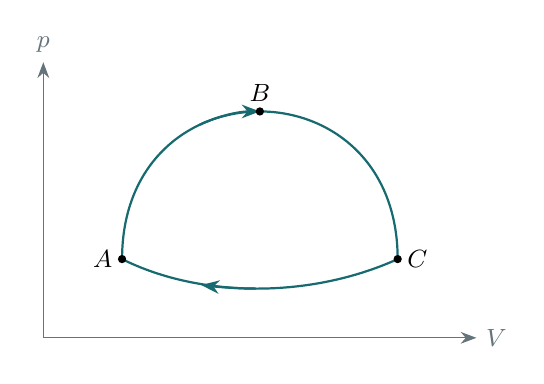
\begin{tikzpicture}[x=1cm,y=1cm,font=\small]
\draw[axis] (0,0)--(5.5,0) node[right] {$V$};
\draw[axis] (0,0)--(0,3.5) node[above] {$p$};
\draw[traj] (1,1) .. controls (1,3.5) and (4.5,3.5) .. (4.5,1)
 .. controls (3.4,.5) and (2,.5) .. (1,1);
\draw[motion] (1.986125,2.70625) .. controls (2.225,2.82) and (2.49,2.875) .. (2.75,2.875);
\draw[motion] (2.705,.625) .. controls (2.48,.625) and (2.23,.645) .. (2.006,.67);
\fill (1,1) circle(1.5pt) node[left] {$A$};
\fill (2.75,2.875) circle(1.5pt) node[above] {$B$};
\fill (4.5,1) circle(1.5pt) node[right] {$C$};
\end{tikzpicture}\figcaption{图 热2.1　闭合路径包围非零面积；箭头给出循环方向。}\end{minipage}\end{center}

\Needspace{5\baselineskip}

\pdfbookmark[3]{题型定位}{q1-h0}

\subsection*{题型定位}

对固定系统的闭合准静态循环使用第一定律。非零有向面积给非零净功，反设同一有限过程比热后，温度的闭路积分却给净热量零。

\Needspace{5\baselineskip}

\pdfbookmark[3]{知识点}{q1-h1}

\subsection*{知识点}

温度和内能是状态函数，一周后变化为零。准静态体积功 $W=\oint p\dd V$ 取图中的有向面积，净热量由 $Q=\Delta U+W$ 给出。过程比热按 $\delta Q=Mc\dd T$ 定义，局部的体积变化率还参与决定 $c$。


\Needspace{5\baselineskip}

\pdfbookmark[3]{物理图像}{q1-h2}

\subsection*{物理图像}

解图热2.1A的上方膨胀与下方压缩围成顺时针面积，上方每一体积处的压强更高，所以对外净功为正。解图热2.1B的左右子回路方向相反，有向面积在整周相消，每一瓣仍分别给出非零净功。

\Needspace{5\baselineskip}

\pdfbookmark[3]{解题入口}{q1-h3}

\subsection*{解题入口}

先从状态复原写 $\Delta U=\Delta T=0$，由循环面积写 $Q=W=\mathcal A$。再反设 $c=c_0$，将它从积分号中提出，得到 $Q=Mc_0\oint\dd T=0$，与非零面积相矛盾。


\Needspace{5\baselineskip}

\pdfbookmark[3]{标准解法}{q1-h4}

\subsection*{标准解法}

\textbf{沿闭合路径列第一定律。}气体一周后回到同一状态，内能是状态函数，因此$\Delta U=0$。解图热2.1A沿$A\to B\to C\to A$运行，有向面积为正，气体对外功
\[W=\oint p\dd V>0.\]
取气体对外功为正，一周的\emph{净}吸热$Q=W>0$。这里各微元吸热取正、放热取负，求和得到净吸热。
\begin{center}\begin{minipage}{0.96\linewidth}\centering
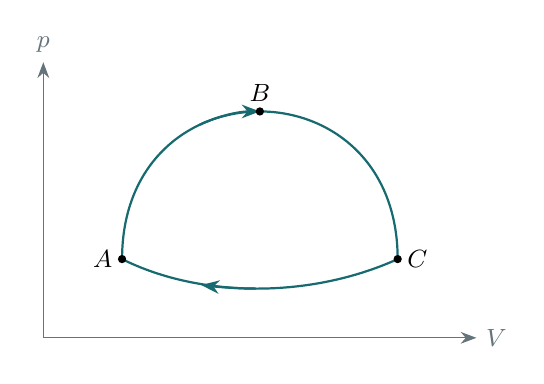
\begin{tikzpicture}[x=1cm,y=1cm,font=\small]
\draw[axis] (0,0)--(5.5,0) node[right] {$V$};
\draw[axis] (0,0)--(0,3.5) node[above] {$p$};
\draw[traj] (1,1) .. controls (1,3.5) and (4.5,3.5) .. (4.5,1)
 .. controls (3.4,.5) and (2,.5) .. (1,1);
\draw[motion] (1.986125,2.70625) .. controls (2.225,2.82) and (2.49,2.875) .. (2.75,2.875);
\draw[motion] (2.705,.625) .. controls (2.48,.625) and (2.23,.645) .. (2.006,.67);
\fill (1,1) circle(1.5pt) node[left] {$A$};
\fill (2.75,2.875) circle(1.5pt) node[above] {$B$};
\fill (4.5,1) circle(1.5pt) node[right] {$C$};
\end{tikzpicture}\figcaption{解图 热2.1A　循环面积给净功，闭合状态给内能增量；净热量由两者确定。}\end{minipage}\end{center}
反设每一微小过程的比热均为同一个有限常量$c$，则
\[\delta Q=Mc\dd T,\qquad Q=\oint\delta Q=Mc\oint\dd T.\]
温度也为状态量，闭合路径满足$\oint\dd T=0$，遂有$Q=0$，与$Q=W>0$矛盾。因此$c$不可能沿全循环保持同一有限值。

\textbf{反向循环与自交路径。}反向循环时$W<0$、$Q<0$，仍与反设的$Q=0$矛盾。若路径自交，只需总有向面积非零，即$W\ne0$，证明仍成立；面积相消为零时，整体积分给 $Q=W=0$，对非零面积的闭合子回路可分别使用同一论证。温度瞬时不变而热量微元不为零处，比热还可能无定义或发散。论证所用的状态函数、固定系统和第一定律也适用于具有这些条件的其他热力学系统。
\subsubsection*{把每一微元与闭路积分对应起来}
把解图热2.1A的循环依次分成足够短的过程段，以$T_i$表示分点温度。
各段温度变化满足
\[
\sum_i(T_{i+1}-T_i)=T_{\rm f}-T_{\rm i}=0.
\]
温差逐项相消，只使用了初、末状态相同。实际热量应为
$Q_{\rm net}=\sum_i\delta Q_i$；只有在反设$c_i=c_0$处处为同一有限值后，才能写成
\[
Q_{\rm net}=\lim\sum_i Mc_i(T_{i+1}-T_i)
=Mc_0(T_{\rm f}-T_{\rm i})=0.
\]
一般过程中各段的 $c_i$ 随状态及路径变化，热量相加时各自与对应温差相乘。
顺时针非零面积$\mathcal A$给$Q_{\rm net}=W_{\rm cyc}=\mathcal A>0$，
反向则给$-\mathcal A$；两种方向都与恒定有限比热的积分结果矛盾。

还可从局部第一定律看出图中各点的过程比热怎样产生。
对准静态理想气体，$c_V$按单位质量计，有
\[
\delta Q=Mc_V\dd T+p\dd V,\qquad
c=c_V+\frac pM\frac{\dd V}{\dd T}\quad(\dd T\ne0).
\]
同一种气体的$c_V$可以是常量，沿路径的$c$仍因$\dd V/\dd T$变化。
等温段若有$p\dd V\ne0$，则$\dd T=0$而$\delta Q\ne0$，此处无法定义有限$c$；
绝热且$\dd T\ne0$的段则有$c=0$。

\begin{center}\begin{minipage}{0.96\linewidth}\centering
\begin{tikzpicture}[x=1cm,y=1cm]
\draw[axis] (0,0)--(6,0) node[right] {$V$};
\draw[axis] (0,0)--(0,3.7) node[above] {$p$};
\coordinate (C) at (3,2);
\draw[traj] (C)--(1,3)--(1,1)--cycle;
\draw[traj] (C)--(5,3)--(5,1)--cycle;
\draw[motion] (1,2.6)--(1,1.7);
\draw[motion] (5,2.6)--(5,1.7);
\fill (C) circle(1.7pt) node[above] {$C$};
\node at (1.7,2) {$W_L<0$};
\node at (4.3,2) {$W_R>0$};
\node[below,align=center] at (3,.65) {两瓣面积相等，$W_L+W_R=0$};
\end{tikzpicture}
\figcaption{解图 热2.1B　同一交点$C$把自交路径分成两个非零净功的闭合子回路。}
\end{minipage}\end{center}
解图热2.1B的两个叶瓣各自围成非零面积，分别对应净功非零的闭合过程。
对全路径积分得到$0=0$时，前面的整体反证没有矛盾；
但左瓣从$C$出发又回到$C$，本身已满足$\Delta U_L=\Delta T_L=0$、
$Q_L=W_L\ne0$。单独对左瓣使用同一反证，便能排除全路径处处同一有限$c$。
整体积分由两瓣的有向面积相消给出 $0=0$，单瓣积分则分别给出非零净热量，提供了更细的路径信息。
相反，等压线上往返的每一闭合段都没有净面积，理想气体可始终取$c=c_p$。
推广到其他物质时，所需条件仍是明确的温度、内能状态和第一定律；
每次积分均跟随同一固定质量和组成的系统，初、末状态由该系统的一组状态量确定。


\Needspace{5\baselineskip}

\pdfbookmark[3]{关键洞察}{q1-h5}

\subsection*{关键洞察}

同一个有限常量乘温度的全微分，使闭路热量为零；第一定律则将实际净热量联系到有向面积。整体面积相消时，可以从同一交点分出独立闭合的非零面积子回路，逐瓣应用这个结论。

\Needspace{5\baselineskip}

\pdfbookmark[3]{易错点}{q1-h6}

\subsection*{易错点}

\begin{itemize}
\item $\oint\dd T=0$ 来自各段升温和降温相抵，局部 $\dd T$ 仍可非零。
\item 有向面积给 $Q_{\rm net}=Q_{\rm in}-Q_{\rm out}$，吸热总量还需各段热量。
\item 理想气体的 $c_V,c_p$ 可为常量，路径比热还含 $p\dd V/(M\dd T)$。
\item 自交点所对应的完整状态相同，才可在那里分出闭合子回路。
\end{itemize}

\Needspace{5\baselineskip}

\pdfbookmark[3]{课堂讲解建议}{q1-h7}

\subsection*{课堂讲解建议}

从解图热2.1A的 $A$ 点走完一周，先让学生指出恢复初值的状态量，再用相同体积处的两条路径比较净功。将温差写成相邻分点的差并逐项相加，在反设 $c_i=c_0$ 后提出常量，完成反证。

接着看解图热2.1B，先对整周相加，再单独沿左瓣返回 $C$，比较这两次积分分别包含哪一块面积。用变图热2.1V1的非闭合等压线作比较，说明有限温差怎样给出常比热过程的非零热量。

\Needspace{5\baselineskip}

\pdfbookmark[3]{变式训练}{q1-h8}

\subsection*{变式训练}

\begin{enumerate}
\item 取非闭合等压膨胀，从 $T_a$ 到 $T_b>T_a$。变图热2.1V1中，功为水平线下的矩形面积。用 $\nu=M/\mu$，
\[
W=p(V_b-V_a)=\nu R(T_b-T_a),\quad
\Delta U=Mc_V(T_b-T_a),\quad Q=Mc_p(T_b-T_a).
\]
因此 $c=c_p$ 可以沿全段保持有限常量。此时温度积分为 $T_b-T_a$，初末状态之间的温差提供非零净热量。
\begin{center}\begin{minipage}{.98\linewidth}\centering
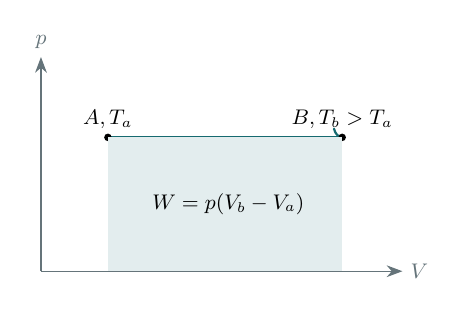
\begin{tikzpicture}[scale=.85,transform shape]
\draw[axis](0,0)--(5.4,0)node[right]{$V$};
\draw[axis](0,0)--(0,3.2)node[above]{$p$};
\draw[traj,->](1,2)--(4.5,2);
\fill(1,2)circle(1.6pt)node[above]{$A,T_a$};
\fill(4.5,2)circle(1.6pt)node[above]{$B,T_b>T_a$};
\fill[accent!12](1,0)rectangle(4.5,2);
\node at(2.8,1){$W=p(V_b-V_a)$};
\end{tikzpicture}
\figcaption{变图热2.1V1\quad 非闭合等压膨胀具有有限温差与有限常量比热}
\end{minipage}\end{center}
\item 一族简单循环的面积 $\mathcal A$ 趋于零。变图热2.1V2中，固定水平宽度并逐次缩小高度差，每个矩形仍有 $W=\Delta p\,\Delta V=\mathcal A>0$。若该循环处处取 $c_0$，闭路积分仍给
\[
Q=Mc_0\oint\dd T=0,
\]
与该成员的 $Q=\mathcal A$ 矛盾。严格取零面积时可退化为等压线往返，去程与回程热量相消，沿途均可有 $c=c_p$。
\begin{center}\begin{minipage}{.98\linewidth}\centering
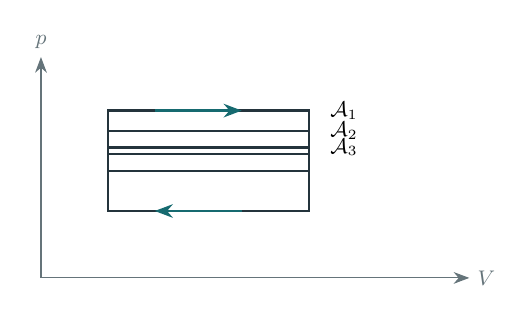
\begin{tikzpicture}[scale=.85,transform shape]
\draw[axis](0,0)--(6.4,0)node[right]{$V$};
\draw[axis](0,0)--(0,3.3)node[above]{$p$};
\foreach \y/\h/\lab in {1/1.5/{\mathcal A_1},1.6/.6/{\mathcal A_2},1.85/.1/{\mathcal A_3}}{
\draw[object](1,\y)rectangle(4,{\y+\h});
\node[right]at(4.2,{\y+\h}){$\lab$};}
\draw[motion](1.7,2.5)--(3,2.5);
\draw[motion](3,1)--(1.7,1);
\end{tikzpicture}
\figcaption{变图热2.1V2\quad 面积逐渐缩小的循环，每一个非零面积仍给非零净功}
\end{minipage}\end{center}
\item 将循环反向运行。变图热2.1V3中，上方路径改为压缩，下方改为膨胀，故 $W'=-\mathcal A,Q'=-\mathcal A$。局部路径反向时，
\[
\delta Q'=-\delta Q,\qquad\dd T'=-\dd T,\qquad
c'=\frac{\delta Q'}{M\dd T'}=\frac{\delta Q}{M\dd T}=c
\]
适用于 $\dd T\ne0$ 的位置。因此反向改变热量与温差的方向，有限的局部比热值在同一点保持，闭路矛盾仍成立。
\begin{center}\begin{minipage}{.98\linewidth}\centering
\begin{tikzpicture}[scale=.85,transform shape]
\draw[axis](0,0)--(5.7,0)node[right]{$V$};
\draw[axis](0,0)--(0,3.7)node[above]{$p$};
\draw[traj](1,1)rectangle(4.5,2.8);
\draw[motion](4,2.8)--(2.8,2.8);
\draw[motion](1.6,1)--(2.8,1);
\node at(2.8,1.85){$W=-\mathcal A$};
\end{tikzpicture}
\figcaption{变图热2.1V3\quad 反向循环将净功和净热量同时反号}
\end{minipage}\end{center}
\item 推广到非理想气体的固定封闭系统。变图热2.1V4先列状态复原，再列全部功。即使内能依赖温度和体积，回到同一状态也有 $\Delta U=0$。当温度复原且总功非零时，
\[
Q=W_{\rm total}\ne0,\qquad
c=c_0\ \Longrightarrow\ Q=Mc_0\oint\dd T=0.
\]
若还有电功等能量传递，$W_{\rm total}$ 包含相应功，正负号统一按系统对外做功规定。非零的 $p$—$V$ 面积单独给出体积功这一项。
\begin{center}\begin{minipage}{.98\linewidth}\centering
\begin{tikzpicture}[scale=.85,transform shape]
\node[draw,align=center]at(0,0){同一固定系统\\初末状态相同};
\draw[motion](2,0)--(3,0);
\node[draw,align=left]at(5.2,0){$\Delta U=0,\ \oint\dd T=0$\\$Q=W_{\rm total}$};
\draw[force](5.2,-.7)--(5.2,-1.8);
\node[align=center]at(5.2,-2.35){总功非零时，恒定有限$c$\\给出的$Q=0$产生矛盾};
\end{tikzpicture}
\figcaption{变图热2.1V4\quad 用固定系统的状态复原和全部功建立同一论证}
\end{minipage}\end{center}
\item 给定循环面积 $\mathcal A>0$，讨论吸热总量。按放热量的正大小记 $Q_{\rm out}=q\ge0$，由净热量关系，
\[
Q_{\rm in}-q=\mathcal A,\quad Q_{\rm in}=\mathcal A+q,\quad
\eta=\frac{\mathcal A}{\mathcal A+q}.
\]
变图热2.1V5的直线上各点具有相同差值。确定热机的吸热量或效率，还需给出 $q$ 或各段传热过程，才能选定这条线上的具体点。
\begin{center}\begin{minipage}{.98\linewidth}\centering
\begin{tikzpicture}[scale=.85,transform shape]
\draw[axis](0,0)--(6.4,0)node[right]{$Q_{\rm out}$};
\draw[axis](0,0)--(0,3.8)node[above]{$Q_{\rm in}$};
\draw[traj](0,1)--(5.2,3.6);
\fill(2,2)circle(1.6pt)node[above left]{$(\,q,\mathcal A+q\,)$};
\draw[<->](2,1)--(2,2)node[midway,right]{$\mathcal A$};
\draw[guide](0,0)--(5.2,2.6);
\end{tikzpicture}
\figcaption{变图热2.1V5\quad 相同净热量只确定两项之差，允许不同的吸放热总量}
\end{minipage}\end{center}
\item 循环包含理想气体的等温膨胀段。变图热2.1V6中，沿双曲线体积增加而 $T=T_*$ 恒定，所以
\[
\dd U=0,\quad \delta Q=p\dd V,\quad
Q_{ab}=\nu RT_*\ln(V_b/V_a)>0.
\]
这一整段有非零热量而 $\dd T=0$，过程比热的有限定义在此不成立。若温度只在孤立位置驻定，则同时求该处热量微元的阶数，利用它与温度微元之比判断局部极限。
\begin{center}\begin{minipage}{.98\linewidth}\centering
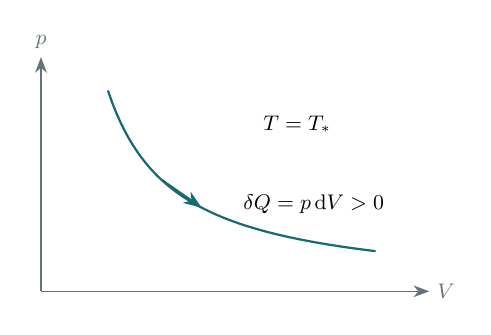
\begin{tikzpicture}[scale=.85,transform shape]
\draw[axis](0,0)--(5.8,0)node[right]{$V$};
\draw[axis](0,0)--(0,3.5)node[above]{$p$};
\draw[traj,domain=1:5,samples=65]plot(\x,{3/\x});
\draw[motion](1.8,1.666667)--(2.4,1.25);
\node[right]at(3.2,2.5){$T=T_*$};
\node[right]at(2.9,1.3){$\delta Q=p\dd V>0$};
\end{tikzpicture}
\figcaption{变图热2.1V6\quad 等温膨胀有热量传递，温度微元为零}
\end{minipage}\end{center}
\item 在一段温度单调的路径上给定有限常量比热 $c_0$。沿途累计热量满足变图热2.1V7中的直线，
\[
Q(T)-Q(T_a)=Mc_0(T-T_a).
\]
若补充回程仍保持同一个 $c_0$，最终回到 $T_a$ 后，累计热量也回到起点，故 $Q_{\rm net}=0,W_{\rm net}=0$。要使闭合后的净功非零，回程中需有局部比热取其他值或有限比热定义失效的过程。
\begin{center}\begin{minipage}{.98\linewidth}\centering
\begin{tikzpicture}[scale=.85,transform shape]
\draw[axis](0,0)--(5.8,0)node[right]{$T$};
\draw[axis](0,0)--(0,3.5)node[above]{$Q$（沿途累计）};
\draw[traj,->](1,.5)--(4.6,2.7);
\draw[guide,->](4.6,2.7)--(1,.5);
\node[above]at(3,2.5){斜率$Mc_0$};
\fill(1,.5)circle(1.5pt)node[below]{$A$};
\fill(4.6,2.7)circle(1.5pt)node[right]{$B$};
\end{tikzpicture}
\figcaption{变图热2.1V7\quad 同一有限常量比热使累计热量在闭合温度后回到初值}
\end{minipage}\end{center}
\item 解图热2.1B的两瓣面积相等而方向相反。变图热2.1V8将交点记为同一完整热力学状态 $C$。整周给 $Q=W=0$，而单独左瓣有
\[
\Delta U_L=\Delta T_L=0,\qquad Q_L=W_L=-\mathcal A\ne0.
\]
因此常量有限比热的假设在左瓣上已产生矛盾；右瓣同样如此。选择子回路时用完整状态的复原判断闭合，组成等状态量也包含在这项条件中。
\begin{center}\begin{minipage}{.98\linewidth}\centering
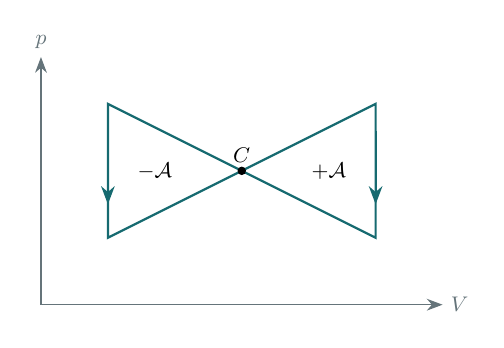
\begin{tikzpicture}[scale=.85,transform shape]
\draw[axis](0,0)--(6,0)node[right]{$V$};
\draw[axis](0,0)--(0,3.7)node[above]{$p$};
\draw[traj](3,2)--(1,3)--(1,1)--cycle;
\draw[traj](3,2)--(5,3)--(5,1)--cycle;
\draw[motion](1,2.6)--(1,1.5);
\draw[motion](5,2.6)--(5,1.5);
\fill(3,2)circle(1.8pt)node[above]{$C$};
\node at(1.7,2){$-\mathcal A$};
\node at(4.3,2){$+\mathcal A$};
\end{tikzpicture}
\figcaption{变图热2.1V8\quad 整周的面积相消，每瓣分别构成非零净功的闭合回路}
\end{minipage}\end{center}
\end{enumerate}

\clearpage

\pdfbookmark[2]{第 2 题 平移等温线确定过程比热曲线}{q2}

\section*{第 2 题\quad 平移等温线确定过程比热曲线}

质量为$M$、摩尔质量为$\mu$的理想气体，定容比热$c_V$为常量。其准静态过程$x$在$p-V$平面上向下平移$p_0>0$后，恰成为温度$T_0$的等温线。求过程$x$的温度下限及其在曲线上的位置；导出$c$与$p$的关系，画出$c-p$曲线。

\begin{center}\begin{minipage}{0.96\linewidth}\centering
\begin{tikzpicture}[x=1cm,y=1cm,font=\small]\draw[axis] (0,0)--(5.5,0) node[right] {$V$};\draw[axis] (0,0)--(0,3.5) node[above] {$p$};
\draw[traj,domain=.65:5,samples=60] plot (\x,{1+1.6/\x});\draw[guide,domain=.65:5,samples=60] plot (\x,{1.6/\x});\draw[<->] (3,.533)--(3,1.533) node[right,midway]{$p_0$};\node[right] at (4.7,1.5) {$x$};\node[right] at (3.7,.25) {$T=T_0$};
\end{tikzpicture}\figcaption{图 热2.2　实线向下平移$p_0$成为等温虚线，同一体积处比较压强。}\end{minipage}\end{center}

\Needspace{5\baselineskip}

\pdfbookmark[3]{题型定位}{q2-h0}

\subsection*{题型定位}

先由过程线在同体积处的压强平移得到路径方程，再用状态方程求温度，沿路径微分第一定律求过程比热。

\Needspace{5\baselineskip}

\pdfbookmark[3]{知识点}{q2-h1}

\subsection*{知识点}

路径满足 $(p-p_0)V=\nu RT_0$，状态满足 $pV=\nu RT$。温度随体积线性增加，压强随体积下降。质量比热的膨胀作功部分为 $(p/M)\dd V/\dd T$，有限过程热量由变比热积分给出。


\Needspace{5\baselineskip}

\pdfbookmark[3]{物理图像}{q2-h2}

\subsection*{物理图像}

解图热2.2A的竖线连接同体积的 $P$ 与 $P_0$，其压强差为 $p_0$。沿实线向右下走，$V,T$ 增加而 $p,c$ 下降。解图热2.2B的空心端点为大体积极限，低温极限则位于 $p$ 很大的另一端。

\Needspace{5\baselineskip}

\pdfbookmark[3]{解题入口}{q2-h3}

\subsection*{解题入口}

将两个状态方程相减，得 $p_0V=\nu R(T-T_0)$，从而 $\dd V/\dd T=\nu R/p_0$。把它代入 $\delta Q=Mc_V\dd T+p\dd V$，得到 $c(p)$，再以 $V>0$ 确定 $p>p_0,T>T_0$。


\Needspace{5\baselineskip}

\pdfbookmark[3]{标准解法}{q2-h4}

\subsection*{标准解法}

\textbf{由同体积两点写方程。}设$\nu=M/\mu$。解图热2.2A中同一体积V上的两点压差为$p_0$，较低点在$T_0$等温线上：
\[(p-p_0)V=\nu RT_0,\qquad pV=\nu RT.\]
两式相减，或消去V，分别得到
\[T=T_0+\frac{p_0V}{\nu R},\qquad
V=\frac{\nu R}{p_0}(T-T_0),\qquad p=\frac{p_0T}{T-T_0}.\]
\begin{center}\begin{minipage}{0.96\linewidth}\centering
\begin{tikzpicture}[x=1cm,y=1cm,font=\small]
\draw[axis] (0,0)--(5.5,0) node[right] {$V$};
\draw[axis] (0,0)--(0,3.8) node[above] {$p$};
\draw[traj,domain=.65:5,samples=70] plot (\x,{1+1.6/\x});
\draw[guide,domain=.65:5,samples=70] plot (\x,{1.6/\x});
\draw[guide] (0,1) node[left] {$p_0$}--(5.1,1);
\node[below] at (4.1,.39) {$T_0$等温线};
\draw[guide] (2,0) node[below] {$V$}--(2,1.8);
\fill (2,.8) circle(1.5pt) node[below left] {$P_0$};
\fill (2,1.8) circle(1.5pt) node[above left] {$P$};
\draw[<->] (2.18,.8)--(2.18,1.8) node[midway,right] {$p_0$};
\fill (1,2.6) circle(1.5pt) node[above right] {$A$};
\fill (4,1.4) circle(1.5pt) node[above right] {$B$};
\draw[motion] (2.9,{1+1.6/2.9})--(3.4,{1+1.6/3.4});
\node[align=center] at (3.6,3.1) {$T=T_0+p_0V/(\nu R)$\\$V\to0^+:T\to T_0^+$};
\end{tikzpicture}\figcaption{解图 热2.2A\quad 同一$V$处，实线状态与$T_0$等温线状态的压强差为$p_0$；有限体积时$T>T_0$。}\end{minipage}\end{center}
物理区域为$V>0$、$p>p_0$，故$T>T_0$。随V增加，T单调增加；整条曲线的温度下限为$T_0$，只在左上方$V\to0^+$、$p\to\infty$时趋近，该端点为不取到的极限。若只取图上的有限曲线段，最低温度在其左上端，且大于$T_0$。

\textbf{由温度微元求比热。}这里$c_V,c$按单位质量计，故
\[\dd V=\frac{MR}{\mu p_0}\dd T,\qquad
\delta Q=Mc_V\dd T+p\dd V
=M\left(c_V+\frac{Rp}{\mu p_0}\right)\dd T.\]
可把所得热容量看成两项的和：单位质量升温$\dd T$使内能增加$c_V\dd T$，同时沿图热2.2A的平移曲线膨胀，对外功为
\[\frac{p\dd V}{M}=\frac{Rp}{\mu p_0}\dd T.\]
这条路径的单位质量体积变化率为 $R/(\mu p_0)$，相应作功项随当前压强 $p$ 增加。当$p$很大时，同样的温升仍对应相同的体积增量，却要克服更大的压强，所需热量便更多。

于是
\result{c(p)=c_V+\frac{R}{\mu p_0}p,\qquad p>p_0.}
\begin{center}\begin{minipage}{0.96\linewidth}\centering
\begin{tikzpicture}[x=1cm,y=1cm,font=\small]\draw[axis] (0,0)--(5.5,0) node[right] {$p$};\draw[axis] (0,0)--(0,3.5) node[above] {$c$};
\draw[traj] (1,1.3)--(4.8,3.2);\draw[guide] (1,0) node[below]{$p_0$}--(1,1.3)--(0,1.3) node[left]{$c_p$};\draw[ink,fill=white] (1,1.3) circle(2pt);\node[align=left] at (3.45,.75) {$p>p_0$\\斜率 $R/(\mu p_0)$};
\end{tikzpicture}\figcaption{解图 热2.2B　只取$p>p_0$的直线部分；端点$c_p$不属于有限体积过程。}\end{minipage}\end{center}
解图热2.2B的$c-p$图为斜率$R/(\mu p_0)$的直线，其实际定义域只取$p>p_0$。当$p\to p_0^+$时$c\to c_V+R/\mu=c_p$；这对应$V\to\infty,T\to\infty$。沿V增大的方向，温度上升、气体作正功且吸热，$c>c_p>0$，与公式相符。
\subsubsection*{两种温度表示及有限过程的热量}
解图热2.2A的竖线连接相同体积的两个状态，设上端为$P$、下端为$P_0$。
$P_0$在$T_0$等温线上，故$(p-p_0)V=\nu RT_0$；
上端$P$的温度为$T$，有$pV=\nu RT$。分别作差和取比，给出
\[
p_0V=\nu R(T-T_0),\qquad
\frac T{T_0}=\frac p{p-p_0}.
\]
因此当$V$由小变大时，$T$按直线规律升高，$p$却沿双曲线下降。
每一条温度高于$T_0$的等温线与过程$x$只交于一个状态；
对应的体积$V=\nu R(T-T_0)/p_0$随温度增加。
若实际过程从有限的$V_a$开始，其最低温度为$T_a$；
只有把整条正体积曲线都作为定义域时，才以$T_0$为不取到的下确界。

将比热写成温度的函数，再分别取低温和高温极限。
由$p/p_0=T/(T-T_0)$，有
\[
c(T)=c_V+\frac R\mu\frac T{T-T_0}
=c_p+\frac{RT_0}{\mu(T-T_0)},\qquad T>T_0.
\]
求导得到
\[
\frac{\dd c}{\dd T}=-\frac{RT_0}{\mu(T-T_0)^2}<0,\qquad
\frac{\dd c}{\dd V}=-\frac{\nu R^2T_0}{\mu p_0V^2}<0.
\]
所以$c$随$p$增加而增加，随$V$和$T$增加却减小。
解图热2.2B的左端$c_p$对应很大的体积和温度；左上方的低温极限反而有$c\to+\infty$。
在图中标出两个状态$A,B$，令$0<V_a<V_b$，则
$p_a>p_b>p_0$、$T_b>T_a>T_0$、$c_a>c_b>c_p$。

有限膨胀段的比热随温度变化，将 $c(T)$ 沿全段积分求热量。先由体积功求得
\[
\begin{aligned}
W_{a\to b}
&=\int_{V_a}^{V_b}\left(p_0+\frac{\nu RT_0}{V}\right)\dd V\\
&=p_0(V_b-V_a)+\nu RT_0\ln\frac{V_b}{V_a}\\
&=\nu R(T_b-T_a)+\nu RT_0
 \ln\frac{T_b-T_0}{T_a-T_0},\\
\Delta U&=Mc_V(T_b-T_a),\\
Q_{a\to b}&=Mc_p(T_b-T_a)+\nu RT_0
 \ln\frac{T_b-T_0}{T_a-T_0}.
\end{aligned}
\]
也可直接由$M\int_{T_a}^{T_b}c(T)\dd T$得到最后一式。
前一算法用图中$A\to B$曲线下的功面积，后一算法用$c(T)$积分，两者给同一热量。
对膨胀段，上述对数和温差均为正，所以吸热且作正功；反向压缩时二者同时反号，
但局部$c=\delta Q/(M\dd T)$仍为同一正值函数。
例如取$V_b=2V_a$且$V_a=\nu RT_0/p_0$，
则$T_a=2T_0,T_b=3T_0,p_a=2p_0,p_b=3p_0/2$，
\[
W=\nu RT_0(1+\ln2),\qquad
Q=Mc_pT_0+\nu RT_0\ln2.
\]
两端的局部比热分别为 $c_a=c_V+2R/\mu$ 与 $c_b=c_V+3R/(2\mu)$。全段平均比热为 $Q/[M(T_b-T_a)]$，由上式中的对数项确定。
比热的单位是$\mathrm{J/(kg\cdot K)}$，$R/\mu$与$c_V$同量纲；
对数的自变量 $V_b/V_a$ 为同种量的比值，量纲约去。


\Needspace{5\baselineskip}

\pdfbookmark[3]{关键洞察}{q2-h5}

\subsection*{关键洞察}

沿这条曲线，每一相同温升对应同一体积增量，因此当前压强越高，单位温升的对外功越大。$c$ 随 $p$ 上升，随 $V$ 与 $T$ 下降。温度下确界 $T_0$ 与比热下确界 $c_p$ 位于曲线的相反两端。

\Needspace{5\baselineskip}

\pdfbookmark[3]{易错点}{q2-h6}

\subsection*{易错点}

\begin{itemize}
\item 平移发生在压强方向，同体积处有 $p-p_{\rm iso}=p_0$。
\item 质量比热与 $R/\mu$ 相加，摩尔热容量则与 $R$ 相加。
\item 有限膨胀段的作功包含 $\nu RT_0\ln(V_b/V_a)$。
\item 整条曲线的温度下确界在 $V\to0^+$，有限取段的最低温度在实际左端。
\end{itemize}

\Needspace{5\baselineskip}

\pdfbookmark[3]{课堂讲解建议}{q2-h7}

\subsection*{课堂讲解建议}

在解图热2.2A中给 $P,P_0$ 分别写状态方程，让学生用两式之差判断沿曲线膨胀时温度怎样改变。接着在解图热2.2B标出两个实际状态，分别对应较高压强和较高温度，说明比热随哪一个变量增加。

取 $V_b=2V_a$ 并选 $V_a=\nu RT_0/p_0$，逐项求功、内能与热量。由变图热2.2V4中 $p_0$ 缩小时的曲线，对照有限热量与不断增大的局部比热，解释微小温差在两者之间的作用。

\Needspace{5\baselineskip}

\pdfbookmark[3]{变式训练}{q2-h8}

\subsection*{变式训练}

\begin{enumerate}
\item 向下平移量改为 $2p_0$。变图热2.2V1的压强差增倍，两个方程给
\[
(p-2p_0)V=\nu RT_0,\quad T=T_0+\frac{2p_0V}{\nu R},\quad
\frac{\dd V}{\dd T}=\frac{\nu R}{2p_0}.
\]
将体积导数代入第一定律，
\[
c=c_V+\frac{Rp}{2\mu p_0},\qquad p>2p_0.
\]
当 $V\to0^+$ 时温度仍趋于 $T_0$，当 $V\to\infty$ 时压强趋于 $2p_0$、比热趋于 $c_p$。
\begin{center}\begin{minipage}{.98\linewidth}\centering
\begin{tikzpicture}[scale=.85,transform shape]
\draw[axis](0,0)--(6,0)node[right]{$V/V_*$};
\draw[axis](0,0)--(0,4.4)node[above]{$p/p_0$};
\draw[traj,domain=.6:5,samples=80]plot(\x,{2+1/\x});
\draw[guide,domain=.6:5,samples=80]plot(\x,{1/\x});
\draw[<->](3,.333333)--(3,2.333333)node[midway,right]{$2p_0$};
\node[below]at(3,0){$3$};
\end{tikzpicture}
\figcaption{变图热2.2V1\quad 将平移量增倍，实线与等温线在同体积处的间距增倍}
\end{minipage}\end{center}
\item 只用图形和状态方程求温度下确界。相同正体积处实线压强比 $T_0$ 等温线高 $p_0$，有
\[
T-T_0=\frac{p_0V}{\nu R}>0,\qquad
\frac{\dd T}{\dd V}=\frac{p_0}{\nu R}>0 .
\]
变图热2.2V2在温度体积图中画成正斜率直线，其 $V=0$ 处为空心端点。整条正体积曲线取下确界 $T_0$；若取有限段 $V_a\leq V\leq V_b$，最低温度为 $T_a=T_0+p_0V_a/(\nu R)$。
\begin{center}\begin{minipage}{.98\linewidth}\centering
\begin{tikzpicture}[scale=.85,transform shape]
\draw[axis](0,0)--(5.7,0)node[right]{$p_0V/(\nu RT_0)$};
\draw[axis](0,0)--(0,3.5)node[above]{$T/T_0$};
\draw[traj](0,1)--(4.4,3.2);
\filldraw[fill=white](0,1)circle(2pt)node[left]{$1$};
\fill(1,1.5)circle(1.7pt)node[above left]{$A$};
\fill(3,2.5)circle(1.7pt)node[above left]{$B$};
\node[below]at(1,0){$p_0V_a/(\nu RT_0)$};
\end{tikzpicture}
\figcaption{变图热2.2V2\quad 整条正体积曲线与有限取段的最低温度分别由左端确定}
\end{minipage}\end{center}
\item 在 $p=3p_0$ 的状态求温度、体积与比热。将压强代入 $T/T_0=p/(p-p_0)$，再代路径式，
\[
T=\frac32T_0,\qquad V=\frac{\nu RT_0}{2p_0},\qquad
c=c_V+\frac{3R}{\mu}>0 .
\]
变图热2.2V3标出这一状态。沿膨胀方向温度上升、吸热；在同一点沿反向路径，$\dd T,\delta Q$ 同时反号，其比值保持为上述正值。
\begin{center}\begin{minipage}{.98\linewidth}\centering
\begin{tikzpicture}[scale=.85,transform shape]
\draw[axis](0,0)--(5.7,0)node[right]{$V/V_*$};
\draw[axis](0,0)--(0,4.2)node[above]{$p/p_0$};
\draw[traj,domain=.4:5,samples=80]plot(\x,{1+1/\x});
\fill(.5,3)circle(1.8pt)node[above right]{$p=3p_0$};
\draw[guide](.5,0)--(.5,3)--(0,3)node[left]{$3$};
\node[right]at(1.4,2.8){$V_*=\nu RT_0/p_0$};
\node[below]at(.5,0){$1/2$};
\end{tikzpicture}
\figcaption{变图热2.2V3\quad 压强三倍平移量的状态位于较小体积端}
\end{minipage}\end{center}
\item 令 $p_0\to0^+$ 并固定有限正体积区间 $[V_a,V_b]$。温差为 $p_0(V_b-V_a)/(\nu R)$，趋于零；体积功及热量为
\[
W=p_0(V_b-V_a)+\nu RT_0\ln\frac{V_b}{V_a},\qquad
Q=Mc_p\frac{p_0(V_b-V_a)}{\nu R}+\nu RT_0\ln\frac{V_b}{V_a}.
\]
因此二者趋于相同的有限等温热量，而 $c=c_V+Rp/(\mu p_0)$ 发散。变图热2.2V4取 $V_b=2V_a,c_V=3R/(2\mu)$，将热量除以 $\nu RT_0$，将比热除以 $R/\mu$，用同一纵轴刻度表现有限极限与发散。
\begin{center}\begin{minipage}{.98\linewidth}\centering
\begin{tikzpicture}[scale=.85,transform shape]
\draw[axis](0,0)--(5.7,0)node[right]{$\delta=p_0V_a/(\nu RT_0)$};
\draw[axis](0,0)--(0,3.6)node[above]{归一化量};
\draw[traj,domain=0:1,samples=55]plot({5*\x},{.25*(2.5*\x+ln(2))});
\draw[object,dashed,domain=.1:1,samples=85]plot({5*\x},{.25*(2.5+1/\x)});
\node[right]at(4.3,.73){$Q/(\nu RT_0)$};
\node[right]at(2.4,1.12){$c_a/(R/\mu)$};
\node[left]at(0,.25){$1$};\node[left]at(0,2.5){$10$};
\filldraw[fill=white](0,{.25*ln(2)})circle(1.8pt)node[left]{$\ln2$};
\end{tikzpicture}
\figcaption{变图热2.2V4\quad 定体积区间的等温极限中，热量有限，局部比热发散}
\end{minipage}\end{center}
\item 过程只取 $V_a\le V\le V_b$。变图热2.2V5用阴影给出功，
\[
W=\int_{V_a}^{V_b}\left(p_0+\frac{\nu RT_0}{V}\right)\dd V
=p_0(V_b-V_a)+\nu RT_0\ln\frac{V_b}{V_a}.
\]
由温差 $\Delta T=p_0(V_b-V_a)/(\nu R)$ 得 $\Delta U=Mc_V\Delta T$，加到功上得到总热量。温度最小值在 $A$，最大值在 $B$；比热随温度下降，所以最大局部比热在 $A$。
\begin{center}\begin{minipage}{.98\linewidth}\centering
\begin{tikzpicture}[scale=.85,transform shape]
\fill[accent!12](1,0)--(1,2)--plot[domain=1:2,samples=60](\x,{1+1/\x})--(2,0)--cycle;
\draw[axis](0,0)--(4.8,0)node[right]{$V/V_a$};
\draw[axis](0,0)--(0,3.1)node[above]{$p/p_0$};
\draw[traj,domain=.7:4,samples=70]plot(\x,{1+1/\x});
\draw[guide](1,0)--(1,2);\draw[guide](2,0)--(2,1.5);
\node[below]at(1,0){$1$};\node[below]at(2,0){$2$};
\node[right]at(2.7,2.3){阴影面积$W$};
\end{tikzpicture}
\figcaption{变图热2.2V5\quad 有限段功由整个压强曲线下的面积给出}
\end{minipage}\end{center}
\item 从 $V_b$ 沿同一路径压缩到 $V_a<V_b$。变图热2.2V6中的箭头朝左上，体积和温度同时减小。交换有限积分的上下限，
\[
W_{b\to a}=-W_{a\to b},\quad
\Delta U_{b\to a}=-Mc_V(T_b-T_a),\quad
Q_{b\to a}=-Q_{a\to b}.
\]
这一段压缩放热，局部 $\delta Q$ 和 $\dd T$ 都为负，因此 $c=\delta Q/(M\dd T)>c_p>0$。
\begin{center}\begin{minipage}{.98\linewidth}\centering
\begin{tikzpicture}[scale=.85,transform shape]
\draw[axis](0,0)--(5.8,0)node[right]{$V/V_*$};
\draw[axis](0,0)--(0,4)node[above]{$p/p_0$};
\draw[traj,domain=.5:5,samples=85]plot(\x,{1+1/\x});
\draw[motion](3.8,1.263158)--(2.8,1.357143);
\node at(3.2,2.3){压缩，$\dd V<0$};
\node at(3.2,.6){$\dd T<0,\ \delta Q<0$};
\end{tikzpicture}
\figcaption{变图热2.2V6\quad 沿同一路径压缩，温差和热量同时反号}
\end{minipage}\end{center}
\item 将过程改画在温度体积图上。由 $T=T_0+p_0V/(\nu R)$，变图热2.2V7的纵轴截距为 $T_0$，斜率为 $p_0/(\nu R)$。同一正体积处，平移量加倍使温度超过 $T_0$ 的部分加倍。若比较同一压强，则分别用
\[
T_i=\frac{pT_0}{p-p_{0i}},\qquad p>\max(p_{01},p_{02}),
\]
在共同定义域内求值，仍可确定各自温度。
\begin{center}\begin{minipage}{.98\linewidth}\centering
\begin{tikzpicture}[scale=.85,transform shape]
\draw[axis](0,0)--(5.8,0)node[right]{$V/V_*$};
\draw[axis](0,0)--(0,4)node[above]{$T/T_0$};
\draw[traj](0,1)--(4.5,2.8)node[right]{$p_0$};
\draw[object,dashed](0,1)--(3.4,3.72)node[right]{$2p_0$};
\filldraw[fill=white](0,1)circle(1.8pt)node[left]{$1$};
\draw[guide](2,0)--(2,2.6);
\end{tikzpicture}
\figcaption{变图热2.2V7\quad 相同等温基线下，平移量决定温度体积直线的斜率}
\end{minipage}\end{center}
\item 另取实际过程向上平移 $p_0$ 后成为 $T_0$ 等温线。此时
\[
(p+p_0)V=\nu RT_0,\quad
T=T_0-\frac{p_0V}{\nu R},\quad
c=c_V-\frac{Rp}{\mu p_0},
\quad0<V<\frac{\nu RT_0}{p_0}.
\]
变图热2.2V8取 $c_V=3R/(2\mu)$，零比热点为 $p=3p_0/2,V=0.4\nu RT_0/p_0$。膨胀时 $\dd T<0$，较小体积的高压区 $c<0$ 因而吸热，越过零比热点后 $c>0$ 因而放热。正温度、正压强限定该图的实际状态范围。
\begin{center}\begin{minipage}{.98\linewidth}\centering
\begin{tikzpicture}[scale=.85,transform shape]
\draw[axis](0,0)--(5.7,0)node[right]{$V/V_*$};
\draw[axis](0,0)--(0,3.6)node[above]{$p/p_0$};
\draw[traj,domain=.25:1,samples=80]plot({4*\x},{1/\x-1});
\draw[guide](0,1.5)--(4.6,1.5)node[right]{$c=0$};
\fill(1.6,1.5)circle(1.7pt);
\node[below]at(4,0){$1$};
\node[below]at(1.6,0){$0.4$};
\node[right]at(2.7,2.5){$c_V=3R/(2\mu)$};
\end{tikzpicture}
\figcaption{变图热2.2V8\quad 实际过程位于等温线下方，零比热状态分隔膨胀中的吸热和放热}
\end{minipage}\end{center}
\end{enumerate}

\clearpage

\pdfbookmark[2]{第 3 题 直线过程的温度图像与比热正负}{q3}

\section*{第 3 题\quad 直线过程的温度图像与比热正负}

质量为$M$、摩尔质量为$\mu$的理想气体，定容比热$c_V=3R/(2\mu)$。气体沿直线由$A(V_0,2p_0)$到$B(2V_0,p_0)$。求$T(V)$并作图；求过程比热$c(V)$并作图，结合$\delta Q/(M\dd T)$解释各段$c$的正负。

\begin{center}\begin{minipage}{0.96\linewidth}\centering
\begin{tikzpicture}[x=1cm,y=1cm,font=\small]\draw[axis] (0,0)--(5.5,0) node[right] {$V/V_0$};\draw[axis] (0,0)--(0,3.5) node[above] {$p/p_0$};
\draw[traj] (1,2)--(2,1);\draw[motion] (1.25,1.75)--(1.65,1.35);\fill[ink] (1,2) circle(1.4pt);\node[above right] at (1,2) {A};
\fill[ink] (2,1) circle(1.4pt);\node[above right] at (2,1) {B};
\draw[guide] (1,0) node[below]{1}--(1,2)--(0,2) node[left]{2};\draw[guide] (2,0) node[below]{2}--(2,1)--(0,1) node[left]{1};
\end{tikzpicture}\figcaption{图 热2.3　直线连接两端状态；坐标按$V_0,p_0$归一化。}\end{minipage}\end{center}

\Needspace{5\baselineskip}

\pdfbookmark[3]{题型定位}{q3-h0}

\subsection*{题型定位}

负斜率直线上的温度先升后降，过程比热的分母和分子分别在不同位置过零。由状态方程与第一定律分别确定这两个位置，作出两支比热曲线。

\Needspace{5\baselineskip}

\pdfbookmark[3]{知识点}{q3-h1}

\subsection*{知识点}

温度由 $pV$ 决定，温度斜率给单位体积增量的内能变化，压强给单位体积增量的体积功。两项相加得到热量微元，除以 $M\dd T$ 得到过程比热。


\Needspace{5\baselineskip}

\pdfbookmark[3]{物理图像}{q3-h2}

\subsection*{物理图像}

解图热2.3A在 $x=3/2$ 处达到温度顶点。解图热2.3B在此有竖直渐近线，较右侧 $x=15/8$ 处过零。两点之间气体膨胀、吸热、降温，其对外功同时由吸热和内能减少提供。

\Needspace{5\baselineskip}

\pdfbookmark[3]{解题入口}{q3-h3}

\subsection*{解题入口}

令 $x=V/V_0$，由 $A,B$ 写 $p=p_0(3-x)$。对 $T=T_*x(3-x)$ 微分确定温度极值，再从 $\delta Q=Mc_V\dd T+p\dd V$ 求热量微元，按两者的符号分别画曲线。


\Needspace{5\baselineskip}

\pdfbookmark[3]{标准解法}{q3-h4}

\subsection*{标准解法}

\textbf{温度曲线。}由题图两端点，令$x=V/V_0$，$T_*=\mu p_0V_0/(MR)$，则
\[p=p_0(3-x),\qquad T=T_*x(3-x),\qquad 1\le x\le2.\]
这是开口向下的抛物线。$\dd T/\dd x=T_*(3-2x)$，故
\[T_{\max}=\frac94T_*\quad(x=3/2),\qquad T_A=T_B=T_{\min}=2T_*.\]
\begin{center}\begin{minipage}{0.96\linewidth}\centering
\begin{tikzpicture}[x=2.8cm,y=1cm]
\draw[axis] (.8,0)--(2.3,0) node[right] {$x=V/V_0$};
\draw[axis] (.8,0)--(.8,3.1) node[above] {$T/T_*$};
\draw[traj,domain=1:2,samples=70] plot (\x,{\x*(3-\x)});
\draw[guide] (1.5,0) node[below] {$3/2$}--(1.5,2.25)--(.8,2.25) node[left] {$9/4$};
\draw[guide] (.8,2) node[left] {$2$}--(2,2);
\fill (1,2) circle(1.5pt) node[above left] {$A$};
\fill (2,2) circle(1.5pt) node[above right] {$B$};
\draw (1,.04)--(1,-.04) node[below] {$1$};
\draw (2,.04)--(2,-.04) node[below] {$2$};
\fill[accent] (1.5,2.25) circle(1.5pt) node[above] {$T_{\max}$};
\end{tikzpicture}\figcaption{解图 热2.3A\quad 纵轴按温度尺度$T_*=\mu p_0V_0/(MR)$归一化；$x=3/2$处温度最高。}\end{minipage}\end{center}
\textbf{热量微元与转折。}气体沿A到B膨胀，$\dd V>0$。从状态方程和内能式分别有
\[M c_V\dd T=\frac32p_0(3-2x)\dd V,\qquad
p\dd V=p_0(3-x)\dd V.\]
相加得
\[\delta Q=p_0\left(\frac{15}{2}-4x\right)\dd V.\]
题图热2.3上某点的压强决定单位体积增量的功，温度曲线的斜率决定单位体积增量的内能变化。具体写成
\[\frac{\dd U}{\dd V}=\frac32p_0(3-2x),\qquad
\frac{\delta W}{\dd V}=p_0(3-x).\]
从$x=3/2$到$x=15/8$，第一项已为负，第二项仍为正且绝对值更大，因此$\delta Q=\dd U+\delta W>0$。这段过程中内能随温度下降，膨胀功大于吸热量，内能的减少补足两者之差。

因此吸放热转折在$x=15/8$，而温度极大在$x=3/2$，两点不同。用比热定义相除：
\result{c=\frac{R}{\mu}\frac{15-8x}{2(3-2x)}.}
\begin{center}\begin{minipage}{0.96\linewidth}\centering
\begin{tikzpicture}[x=5cm,y=.38cm]
\draw[axis] (.88,0)--(2.18,0) node[right] {$x=V/V_0$};
\draw[axis] (.88,-8)--(.88,9) node[above] {$c/(R/\mu)$};
\node[left] at (.88,0) {$0$};
\draw[guide] (1.5,-8)--(1.5,8.7) node[above] {$3/2$};
\draw[traj,domain=1:1.37,samples=75] plot (\x,{(15-8*\x)/(2*(3-2*\x))});
\draw[traj,domain=1.59:2,samples=90] plot (\x,{(15-8*\x)/(2*(3-2*\x))});
\draw[motion] (1.35,7)--(1.37,7.77);
\draw[motion] (1.62,-4.25)--(1.59,-6.333333);
\fill (1,3.5) circle(1.4pt) node[above left] {$A$};
\fill (2,.5) circle(1.4pt) node[above right] {$B$};
\draw (1,.12)--(1,-.12) node[below] {$1$};
\draw (2,.12)--(2,-.12) node[below] {$2$};
\fill[accent] (1.875,0) circle(1.5pt);
\draw[guide] (1.875,0)--(1.875,-1.6) node[below] {$15/8$};
\node at (1.12,6.4) {$c>0$};
\node at (1.72,-4.5) {$c<0$};
\node at (2.04,3.5) {$c>0$};
\end{tikzpicture}\figcaption{解图 热2.3B　横向实轴为$c=0$，两支在$x=3/2$处不连接；箭头指向被截去的发散部分。}\end{minipage}\end{center}
沿解图热2.3B的两条分支，将温差和热量的符号分别列为
\begin{center}\begin{tabular}{cccc}\toprule
体积区间 & $\dd T$ & $\delta Q$ & $c$\\\midrule
$1<x<3/2$ & $+$ & $+$ & $+$\\
$3/2<x<15/8$ & $-$ & $+$ & $-$\\
$15/8<x<2$ & $-$ & $-$ & $+$\\\bottomrule\end{tabular}\end{center}
在$x\to(3/2)^-$时$c\to+\infty$，从右侧趋近时$c\to-\infty$；极大温度点$\dd T=0$而热量一阶不为零，比热无有限值。在 $x=15/8$ 处 $c=0$，热量微元过零，该点左侧吸热、右侧放热。当地绝热线与直线过程相切。负比热段中气体吸热却降温，是因为对外作功超过吸热量，内能仍减少。在两端代入各自的体积，得 $c_A=7R/(2\mu)$、$c_B=R/(2\mu)$。
\subsubsection*{直线过程中的温度极大点与热量零点}
题图热2.3中，压强随体积线性变化，温度则由沿途各状态的压强与体积之积决定。
直线斜率为$(p_B-p_A)/(V_B-V_A)=-p_0/V_0$，因此
\[
p=2p_0-\frac{p_0}{V_0}(V-V_0)=3p_0-\frac{p_0}{V_0}V.
\]
代入$pV=(M/\mu)RT$，展开为
\[
T=-\frac{\mu p_0}{MRV_0}V^2+\frac{3\mu p_0}{MR}V.
\]
这与前面的$T_*x(3-x)$完全相同，并给出
\[
\dd T=\frac{\mu p_0}{MR}(3-2x)\dd V.
\]
解图热2.3A的抛物线关于$x=3/2$对称，所以两个端点虽温度相等，
中间仍先升温后降温，形成图中的抛物线温度曲线。

在负比热区间，内能变化和膨胀功分别进入热力学第一定律。
取$x=7/4$、$\dd V>0$，有
\[
\dd U=-\frac34p_0\dd V,\qquad
\delta W=\frac54p_0\dd V,\qquad
\delta Q=\frac12p_0\dd V>0.
\]
气体吸入的热量不足以补偿对外作功，故仍降温。
在温度顶点$x=3/2$，$\dd T=0$，但
$\delta Q=(3/2)p_0\dd V$不为零，过程比热无有限值。
在$x_D=15/8$，则
\[
p_D=\frac98p_0,\qquad
\dd U=-\frac98p_0\dd V,\qquad
\delta W=\frac98p_0\dd V,\qquad\delta Q=0.
\]
此点的温度仍在下降，比热恰为零；两种特殊点由不同的微分量决定。

若另画经过$D$的单原子气体可逆绝热线，其局部斜率为
\[
\left.\frac{\dd p}{\dd V}\right|_{\rm ad,D}
=-\gamma\frac{p_D}{V_D}
=-\frac53\frac{(9/8)p_0}{(15/8)V_0}
=-\frac{p_0}{V_0}.
\]
它与题给直线在$D$相切。绝热线在邻近状态满足$pV^{5/3}=\mathrm{const}$，题给过程满足直线关系；两条曲线在$D$处有相同斜率，曲率则不同。

\subsubsection*{各子段的吸热、放热与全程能量变化}
由$\dd V=V_0\dd x$，任意子段的热量为
\[
Q_{a\to b}=p_0V_0
 \left[\frac{15}{2}x-2x^2\right]_{x_a}^{x_b}.
\]
正吸热累计到$D$，放热只发生在$D$之后，故
\[
Q_{\rm in}=\frac{49}{32}p_0V_0,\qquad
Q_{\rm out}=\frac1{32}p_0V_0,\qquad
Q_{\rm net}=\frac32p_0V_0.
\]
这里$Q_{\rm out}$表示放热量的正的绝对值。
另一方面，直线下方梯形面积给
\[
W_{A\to B}=\frac{p_A+p_B}{2}(V_B-V_A)=\frac32p_0V_0,
\]
初、末温度相同给$\Delta U=0$，所以$Q_{\rm net}=W$，与微元积分一致。
末段放热的$1/32$已计入积分，故净热量小于累计吸热量。
比热图上$3/2$处两支分开，$15/8$处平滑穿过零线，端点分别为$7R/(2\mu)$与$R/(2\mu)$；
温度转折、热量变号和两段有限热量因而在图上分别对应不同的位置与面积。


\Needspace{5\baselineskip}

\pdfbookmark[3]{关键洞察}{q3-h5}

\subsection*{关键洞察}

温度顶点由 $\dd T=0$ 给出，比热零点由 $\delta Q=0$ 给出。在 $x=7/4$，每增加 $\dd V$ 的功为 $5p_0\dd V/4$，其中吸热提供 $p_0\dd V/2$、内能减少提供 $3p_0\dd V/4$，对应负过程比热。

\Needspace{5\baselineskip}

\pdfbookmark[3]{易错点}{q3-h6}

\subsection*{易错点}

\begin{itemize}
\item 两端同温只给 $\Delta U=0$，中间温度仍有极大值。
\item 比热符号由 $\delta Q$ 和 $\dd T$ 同时确定。
\item $x=3/2$ 处画两支渐近线，$x=15/8$ 处画平滑的过零点。
\item 累计吸热从 $A$ 积分至 $D$，放热的正大小从 $D$ 至 $B$ 另取绝对值。
\end{itemize}

\Needspace{5\baselineskip}

\pdfbookmark[3]{课堂讲解建议}{q3-h7}

\subsection*{课堂讲解建议}

先由两端的压强体积坐标画直线，再以 $pV$ 的最大值找温度顶点。将 $\dd T/\dd V$ 和 $\delta Q/\dd V$ 分别画在体积轴旁，逐段填入符号。

取变图热2.3V3的 $x=7/4$，让学生从三条直线读出内能变化、功和热量，并按第一定律相加。再看变图热2.3V6的两块有符号面积，从正热量和负热量求净热量，与变图热2.3V5的梯形面积比较。

\Needspace{5\baselineskip}

\pdfbookmark[3]{变式训练}{q3-h8}

\subsection*{变式训练}

\begin{enumerate}
\item 过程改为 $p=p_a+bV$，$p_a>0,b>0$。变图热2.3V1中直线斜率为正，状态方程和导数为
\[
T=\frac{p_aV+bV^2}{\nu R},\qquad
\frac{\dd T}{\dd V}=\frac{p_a+2bV}{\nu R}>0 .
\]
第一定律给
\[
c=c_V+\frac R\mu\frac{p_a+bV}{p_a+2bV}>0.
\]
膨胀时温度上升、内能增加且对外作正功，因此吸热。正体积区间内温度导数恒正，过程比热保持有限。
\begin{center}\begin{minipage}{.98\linewidth}\centering
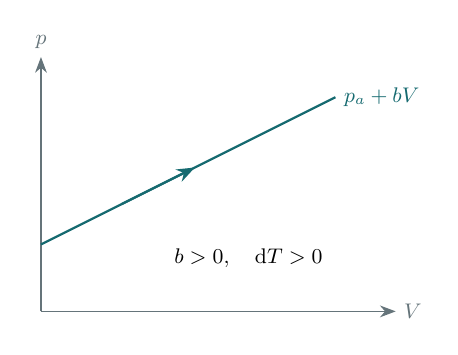
\begin{tikzpicture}[scale=.85,transform shape]
\draw[axis](0,0)--(5.3,0)node[right]{$V$};
\draw[axis](0,0)--(0,3.8)node[above]{$p$};
\draw[traj](0,1)--(4.4,3.2)node[right]{$p_a+bV$};
\draw[motion](1.2,1.6)--(2.3,2.15);
\node at(3.1,.8){$b>0,\quad\dd T>0$};
\end{tikzpicture}
\figcaption{变图热2.3V1\quad 正斜率直线上的膨胀始终升温并吸热}
\end{minipage}\end{center}
\item 只讨论比热的发散点。变图热2.3V2的顶点在 $x=3/2$，此处温度曲线的切线水平，而热量微元为 $3p_0\dd V/2$。令 $x=3/2+\epsilon$，则
\[
\frac{c}{R/\mu}
=\frac{3-8\epsilon}{-4\epsilon}
=2-\frac{3}{4\epsilon}.
\]
因此从左侧趋近时 $c\to+\infty$，从右侧趋近时 $c\to-\infty$。分母的一阶零点与非零分子决定发散方向。
\begin{center}\begin{minipage}{.98\linewidth}\centering
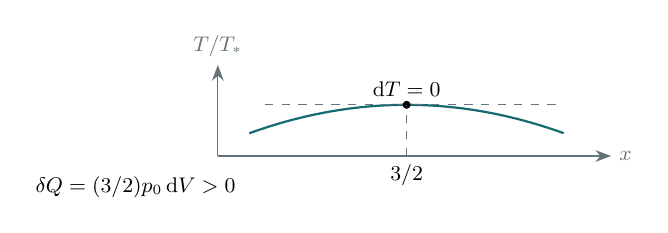
\begin{tikzpicture}[scale=.85,transform shape]
\begin{scope}[x=4.7cm,y=1.7cm]
\draw[axis](.9,1.8)--(2.15,1.8)node[right]{$x$};
\draw[axis](.9,1.8)--(.9,2.6)node[above]{$T/T_*$};
\draw[traj,domain=1:2,samples=75]plot(\x,{\x*(3-\x)});
\draw[guide](1.05,2.25)--(2,2.25);
\fill(1.5,2.25)circle(1.7pt)node[above]{$\dd T=0$};
\draw[guide](1.5,1.8)--(1.5,2.25);
\node[below]at(1.5,1.8){$3/2$};
\end{scope}
\node at(3,2.6){$\delta Q=(3/2)p_0\dd V>0$};
\end{tikzpicture}
\figcaption{变图热2.3V2\quad 温度极值处仍吸热，比热的分母过零而分子保持正值}
\end{minipage}\end{center}
\item 在 $3/2<x<15/8$ 解释负过程比热。变图热2.3V3把第一定律的三项分别画成直线，取 $x=7/4$ 得
\[
\dd U=-\frac34p_0\dd V,\quad
\delta W=\frac54p_0\dd V,\quad
\delta Q=\frac12p_0\dd V .
\]
内能的减少与吸热相加提供对外作功。由于 $\dd T<0$，有 $c=\delta Q/(M\dd T)<0$。图中在 $D$ 左侧，正功曲线的高度大于负内能曲线绝对值，所以热量曲线仍位于零线上方。
\begin{center}\begin{minipage}{.98\linewidth}\centering
\begin{tikzpicture}[scale=.85,transform shape]
\begin{scope}[x=9cm,y=1.1cm]
\draw[axis](1.45,0)--(1.95,0)node[right]{$x$};
\draw[axis](1.45,-1.3)--(1.45,1.9)node[above]{每$\dd V$的能量除以$p_0$};
\draw[traj](1.5,0)--(1.9,-1.2)node[right]{$\dd U/\dd V$};
\draw[object,dashed](1.5,1.5)--(1.9,1.1)node[right]{$\delta W/\dd V$};
\draw[force,-](1.5,1.5)--(1.9,-.1)node[below right]{$\delta Q/\dd V$};
\draw[guide](1.75,-.75)--(1.75,1.25);
\node[below]at(1.75,0){$7/4$};
\end{scope}
\end{tikzpicture}
\figcaption{变图热2.3V3\quad 内能变化与功逐点相加，给出中间的热量直线}
\end{minipage}\end{center}
\item 换为定容比热 $c_V=5R/(2\mu)$ 的双原子气体。状态方程不变，温度顶点仍在 $x=3/2$。热量微元与比热改为
\[
\frac{\delta Q}{\dd V}=\frac{p_0}{2}(21-12x),\qquad
c=\frac R\mu\frac{21-12x}{2(3-2x)}.
\]
变图热2.3V4中，新的热量直线在 $x=7/4$ 过零，负比热区为 $3/2<x<7/4$。更一般地令 $a=\mu c_V/R$，零热量点为 $x_D=3(a+1)/(2a+1)$，温度顶点仍由同一状态路径决定。
\begin{center}\begin{minipage}{.98\linewidth}\centering
\begin{tikzpicture}[scale=.85,transform shape]
\begin{scope}[x=4.8cm,y=.8cm]
\draw[axis](1.4,0)--(2.12,0)node[right]{$x$};
\draw[axis](1.4,-1.6)--(1.4,2.2)node[above]{$(\delta Q/\dd V)/p_0$};
\draw[traj](1.5,1.5)--(2,-.5);
\draw[object,dashed](1.5,1.5)--(2,-1.5);
\fill(1.875,0)circle(1.6pt)node[above right]{$15/8$};
\fill(1.75,0)circle(1.6pt)node[below left]{$7/4$};
\node at(1.74,2.35){实线单原子，虚线双原子};
\end{scope}
\end{tikzpicture}
\figcaption{变图热2.3V4\quad 改变定容比热使热量零点改变，温度顶点保持原位置}
\end{minipage}\end{center}
\item 求全段代数热量。变图热2.3V5的两端压强体积乘积均为 $2p_0V_0$，所以初末温度相同，$\Delta U=0$。图中的梯形面积给
\[
W=\frac{2p_0+p_0}{2}(2V_0-V_0)=\frac32p_0V_0,\qquad Q_{\rm net}=W.
\]
这一结果只用初末同温和内能随温度变化，适用于题设这类定组成理想气体。具体 $c_V$ 改变沿途的吸放热分配。
\begin{center}\begin{minipage}{.98\linewidth}\centering
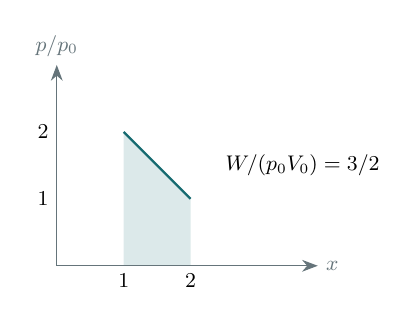
\begin{tikzpicture}[scale=.85,transform shape]
\fill[accent!15](1,0)--(1,2)--(2,1)--(2,0)--cycle;
\draw[axis](0,0)--(3.9,0)node[right]{$x$};
\draw[axis](0,0)--(0,3)node[above]{$p/p_0$};
\draw[traj](1,2)--(2,1);
\node[left]at(0,2){$2$};\node[left]at(0,1){$1$};
\node[below]at(1,0){$1$};\node[below]at(2,0){$2$};
\node[right]at(2.4,1.5){$W/(p_0V_0)=3/2$};
\end{tikzpicture}
\figcaption{变图热2.3V5\quad 初末同温时，梯形功面积等于全段净热量}
\end{minipage}\end{center}
\item 在单原子模型下分别求吸热与放热的正大小。变图热2.3V6按 $\delta Q/\dd V$ 作图，用 $\dd V=V_0\dd x$ 还原热量面积，
\[
Q_{\rm in}=p_0V_0\int_1^{15/8}\left(\frac{15}{2}-4x\right)\dd x
=\frac{49}{32}p_0V_0,
\]
\[
Q_{\rm out}=-p_0V_0\int_{15/8}^2\left(\frac{15}{2}-4x\right)\dd x
=\frac1{32}p_0V_0.
\]
两者之差为 $3p_0V_0/2$，与全段体积功一致。
\begin{center}\begin{minipage}{.98\linewidth}\centering
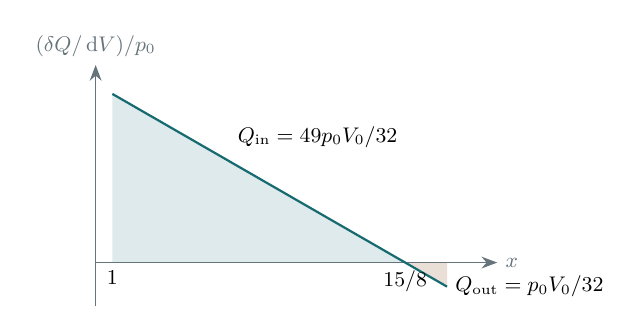
\begin{tikzpicture}[scale=.85,transform shape]
\begin{scope}[x=5cm,y=.72cm]
\fill[accent!14](1,0)--(1,3.5)--(1.875,0)--cycle;
\fill[warm!20](1.875,0)--(2,-.5)--(2,0)--cycle;
\draw[axis](.95,0)--(2.15,0)node[right]{$x$};
\draw[axis](.95,-.9)--(.95,4.1)node[above]{$(\delta Q/\dd V)/p_0$};
\draw[traj](1,3.5)--(2,-.5);
\node[below]at(1,0){$1$};
\node[below]at(1.875,0){$15/8$};
\node[right]at(1.35,2.6){$Q_{\rm in}=49p_0V_0/32$};
\node[right]at(2,-.5){$Q_{\rm out}=p_0V_0/32$};
\end{scope}
\end{tikzpicture}
\figcaption{变图热2.3V6\quad 零热量点把正吸热面积和负放热面积分开}
\end{minipage}\end{center}
\item 画出经过 $D$ 的可逆绝热线。由 $p_D=9p_0/8,V_D=15V_0/8,\gamma=5/3$，
\[
p=p_D\left(\frac{V_D}{V}\right)^{5/3},\qquad
\left.\frac{\dd p}{\dd V}\right|_D
=-\frac53\frac{p_D}{V_D}=-\frac{p_0}{V_0}.
\]
变图热2.3V7中的直线与绝热线在 $D$ 具有相同切线。绝热线二阶导数为 $\gamma(\gamma+1)p/V^2>0$，直线二阶导数为零，所以两曲线在邻近状态分离。
\begin{center}\begin{minipage}{.98\linewidth}\centering
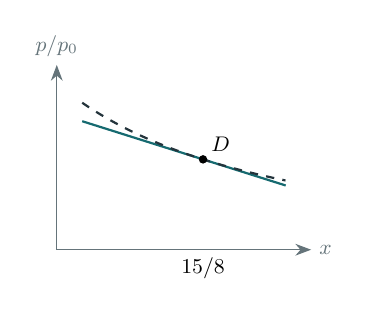
\begin{tikzpicture}[scale=.85,transform shape]
\begin{scope}[x=3.8cm,y=1.2cm]
\draw[axis](1.3,0)--(2.3,0)node[right]{$x$};
\draw[axis](1.3,0)--(1.3,2.3)node[above]{$p/p_0$};
\draw[traj](1.4,1.6)--(2.2,.8);
\draw[object,dashed,domain=1.4:2.2,samples=80]plot(\x,{1.125*pow(1.875/\x,5/3)});
\fill(1.875,1.125)circle(1.8pt)node[above right]{$D$};
\node[below]at(1.875,0){$15/8$};
\end{scope}
\end{tikzpicture}
\figcaption{变图热2.3V7\quad 直线与经过零比热点的绝热线同切线，后者向上弯曲}
\end{minipage}\end{center}
\item 沿 $B\to A$ 反向压缩。变图热2.3V8先从右端升温，过顶点后降温，各点的热量微元也随路径反向改变符号。对于有限的局部比热，
\[
\frac{\delta Q_{\rm rev}}{M\dd T_{\rm rev}}
=\frac{-\delta Q}{M(-\dd T)}=c(V).
\]
原 $D\to B$ 的放热段变为开始时的吸热段。全段 $W=Q=-3p_0V_0/2$，初末温度仍相同，所以 $\Delta U=0$。
\begin{center}\begin{minipage}{.98\linewidth}\centering
\begin{tikzpicture}[scale=.85,transform shape]
\draw[axis](0,0)--(5.4,0)node[right]{$x$};
\draw[axis](0,0)--(0,3.2)node[above]{$T/T_*$};
\draw[traj,domain=1:2,samples=80]plot({2*\x},{\x*(3-\x)});
\draw[motion](3.9,2.0475)--(3.6,2.16);
\draw[motion](2.6,2.21)--(2.2,2.09);
\node[above]at(4,2.3){$B$};
\node[above]at(2,2.1){$A$};
\node[below]at(3,0){$3/2$};
\end{tikzpicture}
\figcaption{变图热2.3V8\quad 反向压缩按同一温度曲线倒行，比热函数在同一状态保持}
\end{minipage}\end{center}
\end{enumerate}

\Needspace{18\baselineskip}

\pdfbookmark[2]{第 4 题 单原子双原子混合理想气体的绝热指数}{q4}

\section*{第 4 题\quad 单原子双原子混合理想气体的绝热指数}

由$\nu_1$ mol单原子气体和$\nu_2$ mol双原子气体组成的理想混合气体，在常温下的准静态绝热方程为$pV^{11/7}=\text{常量}$。忽略双原子分子的振动自由度，求摩尔数比$\alpha=\nu_1/\nu_2$。

\begin{center}\begin{minipage}{0.96\linewidth}\centering
\begin{tikzpicture}[x=1cm,y=1cm,font=\small]\draw[object,fill=accent!6] (0,0) rectangle (6,1.8);\draw[guide] (3,0)--(3,1.8);\node[align=center] at (1.5,.9) {$\nu_1$ mol\\单原子};\node[align=center] at (4.5,.9) {$\nu_2$ mol\\双原子};\node[above] at (3,2.1){两组分混合，温度共同为$T$};
\end{tikzpicture}\figcaption{图 热2.4　图中虚线区分两组分的名称；两种分子均分布在总容积中。}\end{minipage}\end{center}

\Needspace{5\baselineskip}

\pdfbookmark[3]{题型定位}{q4-h0}

\subsection*{题型定位}

由固定组成理想混合物的绝热指数求摩尔比。先将两组分总内能相加，求混合物的摩尔热容量，再由 $C_p/C_V$ 反求组成。

\Needspace{5\baselineskip}

\pdfbookmark[3]{知识点}{q4-h1}

\subsection*{知识点}

常温下单原子气体的有效自由度为3，双原子为5，分别给 $C_{V1}=3R/2,C_{V2}=5R/2$。混合物总热容量为各 $\nu_iC_{Vi}$ 之和，每摩尔热容量除以总摩尔数得到。固定组成下 $C_p-C_V=R$。


\Needspace{5\baselineskip}

\pdfbookmark[3]{物理图像}{q4-h2}

\subsection*{物理图像}

图热2.4中的两组分具有同一温度并均匀分布在总容积中。解图热2.4A的两路内能汇合，解图热2.4B把 $3:1$ 摩尔组成对应的两份热容量分别画为 $9R/2$ 与 $5R/2$，总和为 $7R$。

\Needspace{5\baselineskip}

\pdfbookmark[3]{解题入口}{q4-h3}

\subsection*{解题入口}

由目标指数先算 $C_V/R=1/(\gamma-1)=7/4$，再令 $\alpha=\nu_1/\nu_2$，代入 $(3\alpha+5)/[2(\alpha+1)]$。交叉相乘得到 $6\alpha+10=7\alpha+7$，解得 $\alpha=3$。


\Needspace{5\baselineskip}

\pdfbookmark[3]{标准解法}{q4-h4}

\subsection*{标准解法}

\textbf{两组分内能与热容量。}总摩尔数$\nu=\nu_1+\nu_2$；常温下单、双原子定容摩尔热容量分别为$3R/2$、$5R/2$。解图热2.4A中两份内能相加：
\[U=\frac32\nu_1RT+\frac52\nu_2RT=\nu C_VT,\qquad
C_V=\frac{(3\nu_1+5\nu_2)R}{2(\nu_1+\nu_2)}.\]
\begin{center}\begin{minipage}{0.96\linewidth}\centering
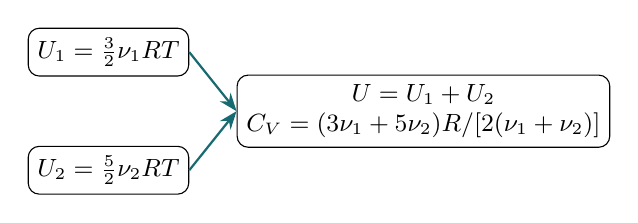
\begin{tikzpicture}[x=1cm,y=1cm,font=\small]\node[draw,rounded corners,align=center] (a) at (0,1.5){$U_1=\frac32\nu_1RT$};\node[draw,rounded corners,align=center] (b) at (0,0){$U_2=\frac52\nu_2RT$};\node[draw,rounded corners,align=center] (c) at (4,.75){$U=U_1+U_2$\\$C_V=(3\nu_1+5\nu_2)R/[2(\nu_1+\nu_2)]$};\draw[motion] (a.east)--(c.west);\draw[motion] (b.east)--(c.west);
\end{tikzpicture}\figcaption{解图 热2.4A　先把两组分总内能相加，再除以总摩尔数求混合气体摩尔热容量。}\end{minipage}\end{center}
定压过程由$p\dd V=\nu R\dd T$与第一定律得到
\[\delta Q=\nu C_V\dd T+p\dd V=\nu(C_V+R)\dd T,\qquad C_p=C_V+R.\]
\textbf{混合气体的绝热方程。}准静态绝热时$\nu C_V\dd T+p\dd V=0$。微分$pV=\nu RT$，消去$\dd T$：
\[(C_V+R)p\dd V+C_VV\dd p=0.\]
除以$C_VpV$，在组分和热容量不变时积分，得
\[\frac{\dd p}{p}+\gamma\frac{\dd V}{V}=0,\qquad
pV^\gamma=\text{常量},\quad\gamma=\frac{C_p}{C_V}.\]
将$\alpha=\nu_1/\nu_2$代入热容量，可直接写出组成与指数的关系：
\[\gamma=1+\frac R{C_V}
=\frac{5\alpha+7}{3\alpha+5}.\]
若$\alpha=0$，只有双原子气体，得$7/5$；若$\alpha\to\infty$，得$5/3$。题给$11/7$位于二者之间，故应有正的有限组成比。解图热2.4A中，各份内能相加得到总热容量，再求两个总热容量之比。这使 $\gamma$ 的组成权重由 $C_V$ 和 $C_p$ 共同决定。

由$\gamma=11/7$反求$C_V=R/(\gamma-1)=7R/4$，再与加权式联立：
\[\frac74=\frac{3\alpha+5}{2(\alpha+1)},\qquad
7(\alpha+1)=2(3\alpha+5).\]
\result{\alpha=3.}
取3 mol单原子与1 mol双原子，$C_V=(9/2+5/2)R/4=7R/4$，$C_p=11R/4$，指数确为11/7。加权依据是摩尔数；若振动自由度激发，$5R/2$不再适用，指数也可能随温度变化。
\subsubsection*{从总热容量逐步得到绝热指数}
解图热2.4A先相加的是两种分子在共同温度下的内能。
用$\mathcal C_V$表示这整份混合气体的定容热容量，用$C_V$表示每摩尔的量，则
\[
\mathcal C_V=\frac{\dd U}{\dd T}
=\nu_1C_{V1}+\nu_2C_{V2},\qquad
C_V=\frac{\mathcal C_V}{\nu_1+\nu_2}.
\]
单原子平动自由度为3，常温双原子取3个平动与2个转动自由度，
所以$C_{V1}=3R/2$、$C_{V2}=5R/2$；题设忽略振动，且混合后组分不反应、不解离。
两种气体均匀分布在同一容积 $V$ 内，各组分的内能按其分子数和共同温度相加。

在定压、组成不变的小过程中，状态方程给
$p\dd V=\nu R\dd T$。按定压摩尔热容量的定义，
\[
C_p=\frac{\delta Q_p}{\nu\dd T}
=\frac{\nu C_V\dd T+p\dd V}{\nu\dd T}
=C_V+R.
\]
若使用整份气体的总热容量，相应关系应是
$\mathcal C_p-\mathcal C_V=\nu R$，对应各摩尔的 $R$ 贡献在整份气体中相加。

再将绝热第一定律和微分状态方程并列：
\[
\nu C_V\dd T=-p\dd V,\qquad
\nu R\dd T=p\dd V+V\dd p.
\]
消去$\nu\dd T$后有
\[
(C_V+R)p\dd V+C_VV\dd p=0,\qquad
C_pp\dd V+C_VV\dd p=0.
\]
除以$C_VpV$，并在组分和有效自由度不变的温区积分：
\[
\ln\frac p{p_a}+\gamma\ln\frac V{V_a}=0,\qquad
pV^\gamma=p_aV_a^\gamma.
\]
因此这里的$\gamma=C_p/C_V$是从同一混合物的两种热容量得到的，
推导中的体积功取 $p\dd V$，对应准静态机械平衡的绝热过程。

\begin{center}\begin{minipage}{0.96\linewidth}\centering
\begin{tikzpicture}[x=1cm,y=1cm]
\fill[accent!16] (0,2) rectangle (2.7,2.5);
\draw[object] (0,2) rectangle (2.7,2.5);
\node[left,align=right] at (-.15,2.25) {单原子3 mol};
\node[right] at (2.8,2.25) {$3\times3R/2=9R/2$};
\fill[warm!16] (0,1) rectangle (1.5,1.5);
\draw[object] (0,1) rectangle (1.5,1.5);
\node[left,align=right] at (-.15,1.25) {双原子1 mol};
\node[right] at (1.6,1.25) {$1\times5R/2=5R/2$};
\fill[accent!16] (0,0) rectangle (2.7,.5);
\fill[warm!16] (2.7,0) rectangle (4.2,.5);
\draw[object] (0,0) rectangle (4.2,.5);
\node[left] at (-.15,.25) {总计4 mol};
\node[right] at (4.3,.25) {$\mathcal C_V=7R$};
\end{tikzpicture}
\figcaption{解图 热2.4B　$3:1$ 组成的两项定容热容量相加为 $7R$，总物质的量为 4 mol，故 $C_V=7R/4$。}
\end{minipage}\end{center}
由$\gamma=11/7$得目标$C_V=7R/4$，由解图热2.4A的加权式得
\[
\frac{3\alpha+5}{2(\alpha+1)}=\frac74
\ \Longrightarrow\ 6\alpha+10=7\alpha+7
\ \Longrightarrow\ \alpha=3.
\]
解图热2.4B 中两条长度相加，得到 $\mathcal C_V=7R$、
$\mathcal C_p=11R$，每摩尔分别为$7R/4$、$11R/4$，两种计量所得指数均为$11/7$。

若将题给指数保留为一般$\gamma$，可得
\[
\alpha=\frac{5\gamma-7}{5-3\gamma},\qquad
\frac{\dd\gamma}{\dd\alpha}=\frac4{(3\alpha+5)^2}>0.
\]
故只有$7/5<\gamma<5/3$对应两组分都存在的正有限摩尔数比。
端点分别对应纯双原子与纯单原子气体，两者之间对应两种正摩尔数的混合。
若转动冻结或振动激发，须先更换各组分的热容量，再讨论幂律能否用同一常指数表示。


\Needspace{5\baselineskip}

\pdfbookmark[3]{关键洞察}{q4-h5}

\subsection*{关键洞察}

总热容量的加法跟随各组分摩尔数，绝热指数则取混合后的两个热容量之比。$\gamma(\alpha)=(5\alpha+7)/(3\alpha+5)$ 单调上升，端点对应纯双原子与纯单原子组成。

\Needspace{5\baselineskip}

\pdfbookmark[3]{易错点}{q4-h6}

\subsection*{易错点}

\begin{itemize}
\item 每摩尔热容量的分母是总摩尔数 $\nu_1+\nu_2$。
\item 质量比先用摩尔质量换成摩尔比，再作热容量加权。
\item 总热容量的差为 $\nu R$，每摩尔热容量的差为 $R$。
\item 所用温区内组成与有效热容量恒定，才由微分绝热关系积分为常指数幂律。
\end{itemize}

\Needspace{5\baselineskip}

\pdfbookmark[3]{课堂讲解建议}{q4-h7}

\subsection*{课堂讲解建议}

先在解图热2.4B逐条求两组分对总热容量的贡献，再除以总摩尔数。让学生以 $C_V$ 和 $C_p$ 两条总量同时作比，解释 $11/7$ 的由来。

用变图热2.4V5、V6读出两种纯气体极限，再给一个区间内的指数反求正摩尔比。最后比较振动自由度充分激发的情况，按变图热2.4V3重新分配各组分，说明组成推断如何依赖所用热容量。

\Needspace{5\baselineskip}

\pdfbookmark[3]{变式训练}{q4-h8}

\subsection*{变式训练}

\begin{enumerate}
\item 加入第三种固定组成理想气体，摩尔分数为 $y_i=\nu_i/\sum\nu_i$，有效自由度为 $f_i$。总内能相加后，
\[
C_V=\frac R2\sum_i y_if_i,\qquad
\gamma=1+\frac2{\sum_i y_if_i}.
\]
例如取 $f_1=3,f_2=5,f_3=6$ 及目标 $\gamma=11/7$，有 $3y_1+5y_2+6y_3=7/2$。再用 $y_1+y_2+y_3=1$ 得 $2y_2+3y_3=1/2$，变图热2.4V1给出满足正组成的整条线段。单个指数提供这一独立约束，尚需额外组成信息才能选定其中一点。
\begin{center}\begin{minipage}{.98\linewidth}\centering
\begin{tikzpicture}[scale=.85,transform shape]
\begin{scope}[x=5cm,y=5cm]
\draw[axis](0,0)--(1.12,0)node[right]{$y_2$};
\draw[axis](0,0)--(0,1.12)node[above]{$y_3$};
\draw[object](0,1)--(1,0);
\draw[traj,line width=1.2pt](.25,0)--(0,.166667);
\fill(.25,0)circle(1.5pt)node[below]{$1/4$};
\fill(0,.166667)circle(1.5pt)node[left]{$1/6$};
\node at(.36,.62){$y_1=1-y_2-y_3$};
\end{scope}
\end{tikzpicture}
\figcaption{变图热2.4V1\quad 给定三个自由度后，一条热容量约束在组成三角形中给出线段}
\end{minipage}\end{center}
\item 给定 $\alpha=1$，两种分子摩尔数相等。直接按摩尔加权，
\[
C_V=\frac{3+5}{2(1+1)}R=2R,\quad C_p=3R,\quad
\gamma=\frac32.
\]
变图热2.4V2同时画出 $\alpha=3$ 时的 $C_V=7R/4,C_p=11R/4$。在相同总摩尔数下，提高单原子摩尔分数使 $C_V$ 降低，而 $C_p-C_V$ 保持 $R$，所以指数上升。
\begin{center}\begin{minipage}{.98\linewidth}\centering
\begin{tikzpicture}[scale=.85,transform shape]
\draw[axis](0,0)--(6.8,0)node[right]{组成};
\draw[axis](0,0)--(0,3.5)node[above]{$C/R$};
\fill[accent!15](1,0)rectangle(2,2);
\fill[warm!15](2,0)rectangle(3,3);
\fill[accent!15](4,0)rectangle(5,1.75);
\fill[warm!15](5,0)rectangle(6,2.75);
\node[below]at(2,0){$\alpha=1$};
\node[below]at(5,0){$\alpha=3$};
\node at(1.5,2.3){$C_V$};\node at(2.5,3.3){$C_p$};
\node[above]at(5,3.55){同类柱相差$R$};
\end{tikzpicture}
\figcaption{变图热2.4V2\quad 两种摩尔组成的热容量先各自求出，再取比}
\end{minipage}\end{center}
\item 双原子振动充分激发，所用温区内有效自由度取 $f_2=7$。变图热2.4V3中，双原子的定容热容量提高，混合热容量变为
\[
C_V=\frac{3\alpha+7}{2(\alpha+1)}R .
\]
同一目标指数 $\gamma=11/7$ 仍要求 $C_V=7R/4$，于是 $6\alpha+14=7\alpha+7$，得 $\alpha=7$。这里将新的有效自由度在整个过程内视为常量；处在激发过渡温区时使用实际的 $C_V(T)$。
\begin{center}\begin{minipage}{.98\linewidth}\centering
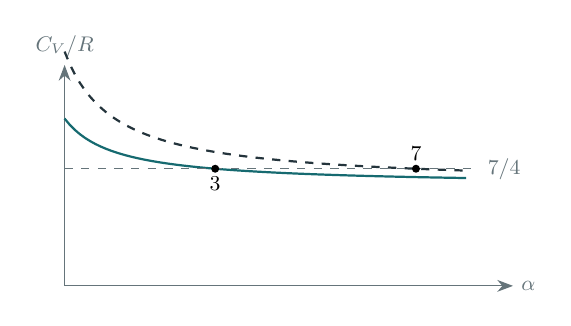
\begin{tikzpicture}[scale=.85,transform shape]
\draw[axis](0,0)--(6.7,0)node[right]{$\alpha$};
\draw[axis](0,0)--(0,3.3)node[above]{$C_V/R$};
\draw[traj,domain=0:8,samples=80]plot({.75*\x},{(3*\x+5)/(2*(1+\x))});
\draw[object,dashed,domain=0:8,samples=80]plot({.75*\x},{(3*\x+7)/(2*(1+\x))});
\draw[guide](0,1.75)--(6.2,1.75)node[right]{$7/4$};
\fill(2.25,1.75)circle(1.7pt)node[below]{$3$};
\fill(5.25,1.75)circle(1.7pt)node[above]{$7$};
\end{tikzpicture}
\figcaption{变图热2.4V3\quad 双原子振动激发后，同一目标热容量对应更大的单原子摩尔比}
\end{minipage}\end{center}
\item 输入质量比 $r_m=m_1/m_2$ 与摩尔质量 $\mu_1,\mu_2$。变图热2.4V4以氦和氮的常温模型说明换算，
\[
\alpha=\frac{m_1/\mu_1}{m_2/\mu_2}
=r_m\frac{\mu_2}{\mu_1},\qquad
\gamma=\frac{5r_m\mu_2/\mu_1+7}{3r_m\mu_2/\mu_1+5}.
\]
取 $\mu_2/\mu_1=7$，目标 $\alpha=3$ 对应 $r_m=3/7$；质量相等时则为 $\alpha=7$。摩尔质量确定质量权重和分子数权重之间的转换。
\begin{center}\begin{minipage}{.98\linewidth}\centering
\begin{tikzpicture}[scale=.85,transform shape]
\draw[axis](0,0)--(5.9,0)node[right]{$r_m=m_1/m_2$};
\draw[axis](0,0)--(0,3.6)node[above]{$\alpha$};
\draw[traj](0,0)--(5,3.5)node[right]{$\mu_2/\mu_1=7$};
\fill(2.142857,1.5)circle(1.7pt);
\draw[guide](0,1.5)node[left]{$3$}--(2.142857,1.5)--(2.142857,0)node[below]{$3/7$};
\end{tikzpicture}
\figcaption{变图热2.4V4\quad 氦与常温氮气的示例中，摩尔比为质量比的七倍}
\end{minipage}\end{center}
\item 取纯单原子极限。变图热2.4V5中 $\alpha$ 增大时，
\[
C_V\to\frac32R,\quad C_p\to\frac52R,\quad
\gamma\to\frac53,\qquad
\frac53-\gamma=\frac4{3(3\alpha+5)}>0 .
\]
最后一式给出与上界的差值，在有限正 $\alpha$ 时为正，随 $\alpha$ 增大趋零。纯单原子端点对应双原子摩尔分数取零。
\begin{center}\begin{minipage}{.98\linewidth}\centering
\begin{tikzpicture}[scale=.85,transform shape]
\begin{scope}[x=.36cm,y=6cm]
\draw[axis](0,1.35)--(18,1.35)node[right]{$\alpha$};
\draw[axis](0,1.35)--(0,1.76)node[above]{$\gamma$};
\draw[guide](0,{5/3})--(16.7,{5/3})node[right]{$5/3$};
\draw[traj,domain=0:16,samples=100]plot(\x,{(5*\x+7)/(3*\x+5)});
\node[below]at(11.5,1.35){单原子占比增加};
\end{scope}
\end{tikzpicture}
\figcaption{变图热2.4V5\quad 单原子摩尔比增大时，绝热指数从下方趋于纯单原子极限}
\end{minipage}\end{center}
\item 取纯双原子极限并确定两种正组分的指数范围。令单原子摩尔分数 $y_1=\alpha/(1+\alpha)$，有
\[
C_V=\frac R2(5-2y_1),\qquad
\gamma=1+\frac2{5-2y_1}.
\]
变图热2.4V6对 $0<y_1<1$ 作图，得到 $7/5<\gamma<5/3$。左端 $y_1=0$ 为纯双原子气体，$C_V=5R/2$。实测指数结合所处温区及有效自由度，决定采用的组成模型。
\begin{center}\begin{minipage}{.98\linewidth}\centering
\begin{tikzpicture}[scale=.85,transform shape]
\begin{scope}[x=5cm,y=8cm]
\draw[axis](0,1.35)--(1.1,1.35)node[right]{$y_1=\nu_1/\nu$};
\draw[axis](0,1.35)--(0,1.72)node[above]{$\gamma$};
\draw[traj,domain=0:1,samples=80]plot(\x,{1+2/(5-2*\x)});
\filldraw[fill=white](0,1.4)circle(1.8pt)node[left]{$7/5$};
\filldraw[fill=white](1,{5/3})circle(1.8pt)node[right]{$5/3$};
\node[below]at(0,1.35){$0$};\node[below]at(1,1.35){$1$};
\end{scope}
\end{tikzpicture}
\figcaption{变图热2.4V6\quad 两组分都存在时的指数位于两个纯气体端点之间}
\end{minipage}\end{center}
\item 给定 $\gamma=3/2$ 并求反解的灵敏度。由 $C_V/R=1/(\gamma-1)=2$ 得 $\alpha=1$。一般反解和导数为
\[
\alpha=\frac{5\gamma-7}{5-3\gamma},\qquad
\frac{\dd\alpha}{\dd\gamma}=\frac4{(5-3\gamma)^2}.
\]
变图热2.4V7取 $\gamma=11/7$ 的切线，其斜率为49。小的测量变化给 $\delta\alpha\simeq49\delta\gamma$；这一线性近似在所取扰动范围内由切线代表曲线，接近纯单原子端时需用完整分式求值。
\begin{center}\begin{minipage}{.98\linewidth}\centering
\begin{tikzpicture}[scale=.85,transform shape]
\begin{scope}[x=17cm,y=.45cm]
\draw[axis](1.39,0)--(1.66,0)node[right]{$\gamma$};
\draw[axis](1.39,0)--(1.39,13)node[above]{$\alpha$};
\draw[traj,domain=1.4:1.64,samples=100]plot(\x,{(5*\x-7)/(5-3*\x)});
\fill({11/7},3)circle(1.6pt)node[above left]{$(11/7,3)$};
\draw[guide]({11/7-.025},1.775)--({11/7+.025},4.225);
\node[right]at(1.50,9){$\dd\alpha/\dd\gamma=49$};
\end{scope}
\end{tikzpicture}
\figcaption{变图热2.4V7\quad 反解曲线向纯单原子端变陡，小的指数变化引起较大的组成变化}
\end{minipage}\end{center}
\item 固定组成，提高双原子的有效自由度。混合热容量增加，$\gamma=1+R/C_V$ 随之降低。若热容量在过程内随温度变化，绝热第一定律给
\[
\int_{T_a}^{T_b}\frac{C_V(T)}T\dd T+R\ln\frac{V_b}{V_a}=0.
\]
变图热2.4V8取 $C_V(T)/R=2+T/(2T_a)$，积分得到 $2\ln(T/T_a)+(T/T_a-1)/2+\ln(V/V_a)=0$。总内能差由 $\nu\int_{T_a}^{T_b}C_V(T)\dd T$ 给出；热容量在温区内恒定时，积分才化为单一幂律。
\begin{center}\begin{minipage}{.98\linewidth}\centering
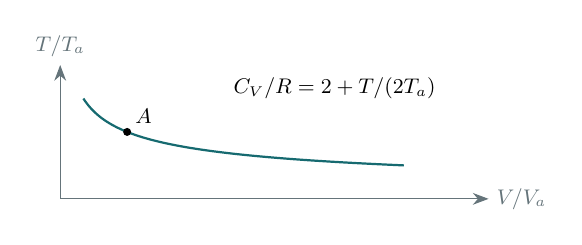
\begin{tikzpicture}[scale=.85,transform shape]
\draw[axis](0,0)--(6.4,0)node[right]{$V/V_a$};
\draw[axis](0,0)--(0,2)node[above]{$T/T_a$};
\draw[traj,domain=.5:1.5,samples=90]plot({pow(\x,-2)*exp(-.5*(\x-1))},{\x});
\fill(1,1)circle(1.7pt)node[above right]{$A$};
\node at(4.1,1.65){$C_V/R=2+T/(2T_a)$};
\end{tikzpicture}
\figcaption{变图热2.4V8\quad 温变热容量的绝热过程由积分关系确定}
\end{minipage}\end{center}
\end{enumerate}

\clearpage

\pdfbookmark[2]{第 5 题 热功效率恒定过程中的总功}{q5}

\section*{第 5 题\quad 热功效率恒定过程中的总功}

1 mol单原子理想气体经历准静态过程，初态$(4p_0,V_0)$，终态$(p_0/4,8V_0)$。每一微小过程的热功比$\delta W/\delta Q$均相同。求全过程气体对外所作的功$W$。

\begin{center}\begin{minipage}{0.96\linewidth}\centering
\begin{tikzpicture}[x=1cm,y=1cm,font=\small]\draw[axis] (0,0)--(5.5,0) node[right] {$V/V_0$};\draw[axis] (0,0)--(0,3.5) node[above] {$p/p_0$};
\draw[traj,domain=1:8,samples=70] plot ({.6*\x},{.75*4/pow(\x,4/3)});\fill[ink] (0.6,3) circle(1.4pt);\node[above right] at (0.6,3) {初态 $(1,4)$};
\fill[ink] (4.8,0.1875) circle(1.4pt);\node[above right] at (4.8,0.1875) {末态 $(8,1/4)$};

\end{tikzpicture}\figcaption{图 热2.5　曲线满足微元热功比恒定；图中横纵比例不同。}\end{minipage}\end{center}

\Needspace{5\baselineskip}

\pdfbookmark[3]{题型定位}{q5-h0}

\subsection*{题型定位}

恒定微元热功比与第一定律共同选定多方路径。用局部约束求过程热容量，再由端点确定指数，最后积分体积功。

\Needspace{5\baselineskip}

\pdfbookmark[3]{知识点}{q5-h1}

\subsection*{知识点}

单原子1 mol气体有 $\dd U=3R\dd T/2$。局部关系 $\delta W=\eta\delta Q$ 给 $(1-\eta)\delta Q=C_V\dd T$。有限变温分支上 $C$ 恒定，进而得到 $pV^n$ 不变；端点温度决定内能差，曲线下面积决定功。


\Needspace{5\baselineskip}

\pdfbookmark[3]{物理图像}{q5-h2}

\subsection*{物理图像}

解图热2.5A中体积从 $V_0$ 增至 $8V_0$，压强下降，温度由 $pV$ 的初末值给出减半。解图热2.5B中吸热为3、输出功为6，内能减少3，单位均为 $p_0V_0$。

\Needspace{5\baselineskip}

\pdfbookmark[3]{解题入口}{q5-h3}

\subsection*{解题入口}

由微元热功比得到 $C=C_V/(1-\eta)$，结合第一定律和状态方程积分为多方。由 $8^n=16$ 得 $n=4/3$，再求 $W=\int p\dd V$。将温差代入 $\Delta U=C_V\Delta T$，得到全程热量。


\Needspace{5\baselineskip}

\pdfbookmark[3]{标准解法}{q5-h4}

\subsection*{标准解法}

\textbf{恒定热功比给出的约束。}记$\eta=\delta W/\delta Q$，$C_V=3R/2$。第一定律为$\delta Q=C_V\dd T+\delta W$，因此
\[(1-\eta)\delta Q=C_V\dd T,\qquad C=\frac{\delta Q}{\dd T}=\frac{C_V}{1-\eta}.\]
本题初末温度不同，所取分支为 $\eta\ne1$，故 $C$ 为有限常量。由$(C-C_V)\dd T=p\dd V=RT\dd V/V$，积分得到
\[\dd\ln T=\frac{R}{C-C_V}\dd\ln V,\quad
TV^{n-1}=\text{常量},\quad pV^n=\text{常量},\]
其中$n=1-R/(C-C_V)$。代初末点：
\[4p_0V_0^n=\frac{p_0}{4}(8V_0)^n,\quad 8^n=16,\quad n=4/3.\]
\begin{center}\begin{minipage}{0.96\linewidth}\centering
\begin{tikzpicture}[x=.62cm,y=.75cm,font=\small]
\fill[accent!12,domain=1:8,samples=70] (1,0)--plot (\x,{4/pow(\x,4/3)})--(8,0)--cycle;
\draw[axis] (0,0)--(9,0) node[right] {$V/V_0$};
\draw[axis] (0,0)--(0,4.55) node[above] {$p/p_0$};
\draw[guide] (0,4) node[left] {$4$}--(1,4)--(1,0) node[below] {$1$};
\draw[guide] (0,.25) node[left] {$1/4$}--(8,.25)--(8,0) node[below] {$8$};
\draw[traj,domain=1:8,samples=70] plot (\x,{4/pow(\x,4/3)});
\fill[accent] (1,4) circle(1.5pt) (8,.25) circle(1.5pt);
\node[align=center] at (5.5,2.8) {$pV^{4/3}=\text{常量}$};
\end{tikzpicture}\figcaption{解图 热2.5A　阴影面积乘 $p_0V_0$ 得对外功。}\end{minipage}\end{center}
解图热2.5A 的坐标分别为 $V/V_0$ 和 $p/p_0$。阴影面积乘 $p_0V_0$ 给出对外功 $W=\int p\dd V$。两端的 $pV$ 给出温差和内能变化，再由 $Q=\Delta U+W$ 求吸热量。这段膨胀中，气体一面吸热，一面降温，吸收的热量和减少的内能共同提供了对外功。

据此
\[C=C_V+\frac{R}{1-n}=-\frac32R,\qquad \eta=1-\frac{C_V}{C}=2.\]
初末温度$T_i=4p_0V_0/R$、$T_f=2p_0V_0/R$，所以
\[\Delta U=-3p_0V_0,\qquad Q=C(T_f-T_i)=3p_0V_0.\]
\result{W=Q-\Delta U=6p_0V_0.}
以$p_0V_0$为能量单位，解图热2.5B左箭头给输入热量，右箭头给输出功；框内同时标出气体自身内能的减少。
\begin{center}\begin{minipage}{0.94\linewidth}\centering
\begin{tikzpicture}[x=1cm,y=1cm]
\node[draw,rounded corners,minimum width=3.7cm,minimum height=1.9cm,align=center] (G) at (0,0)
 {气体\\$\Delta U=-3p_0V_0$};
\draw[force] (-4.8,0)--(G.west) node[midway,above] {$Q=3p_0V_0$};
\draw[motion] (G.east)--(5,0) node[midway,above] {$W=6p_0V_0$};
\node[below,align=center] at (0,-1.15) {$Q-W=\Delta U$；内能减少补足作功所需能量};
\end{tikzpicture}
\figcaption{解图热2.5B\quad 一次降温膨胀的热、功与内能变化；输出功包含释放的内能。}
\end{minipage}\end{center}
解图热2.5B明确了$W/Q=2$的含义。这里气体最终内能较低，若另取回程构成循环，回程的热量和功也计入全周期。

用过程曲线下的面积求对外功，
\[W=\int_{V_0}^{8V_0}4p_0(V_0/V)^{4/3}\dd V
=12p_0V_0(1-8^{-1/3})=6p_0V_0.\]
面积积分同时给出整个过程的正功，数值与吸热量及内能减少量相加相符。
\subsubsection*{恒定微元比值怎样限定整条路径}
设比值$\eta$为同一个有限常数，逐微元写$\delta W=\eta\delta Q$。
若$\eta=0$，准静态正压气体须有$p\dd V=0$，只能等体，
与本题体积增大到8倍不符；若$\eta=1$，第一定律给$\dd U=0$，
理想气体温度恒定，也与端点$pV$减半不符。
因此本题可在$\eta\ne0,1$的分支上定义有限常量
$C=C_V/(1-\eta)$，且$C-C_V\ne0$，前面的除法、积分均有效。

把多方热容量与指数的关系完整展开：
\[
(C-C_V)\dd T=RT\frac{\dd V}{V},\qquad
\frac{\dd T}{T}=\frac{R}{C-C_V}\frac{\dd V}{V}.
\]
记$1-n=R/(C-C_V)$，于是
\[
\ln\frac T{T_i}=(1-n)\ln\frac V{V_i},\qquad
TV^{n-1}=T_iV_i^{n-1}.
\]
将$T=pV/R$代入，便得$pV^n=p_iV_i^n$。反过来，
\[
C=C_V+\frac{R}{1-n}
=\frac{\gamma-n}{1-n}C_V,\qquad
\eta=1-\frac{C_V}{C}
=\frac{\gamma-1}{\gamma-n}.
\]
本题$n=4/3$、$\gamma=5/3$，所以$C=-C_V$、$\eta=2$。
这条路径上 $C=-3R/2$，表示吸热时降温；同一单原子气体的定容热容量为 $C_V=3R/2$。

用$x=V/V_0$把各量写成整条路径上的函数：
\[
p=4p_0x^{-4/3},\qquad
T=\frac{4p_0V_0}{R}x^{-1/3},\qquad
\dd U=-2p_0V_0x^{-4/3}\dd x.
\]
膨胀时$\dd x>0$，而
\[
\delta W=4p_0V_0x^{-4/3}\dd x,\qquad
\delta Q=\dd U+\delta W
=2p_0V_0x^{-4/3}\dd x>0.
\]
两种微元具有相同的 $x^{-4/3}\dd x$ 因子，因此每一位置都有 $\delta W/\delta Q=2$。
由积分得到$Q=3p_0V_0$、$W=6p_0V_0$、$\Delta U=-3p_0V_0$，
也与解图热2.5B标出的能量传递和内能变化相符。

只给端点和总比值 $W/Q=2$ 时，端点仍给 $\Delta U=-3p_0V_0$，第一定律足以求出 $W,Q$。本题用局部条件 $\delta W=2\delta Q$ 确定沿程压强变化；只给总比值时，功和热的积分值保持相同，沿程函数还可以变化。
若加上回程组成循环，整周内能增量为零，净功等于各段有符号热量之和。计算总吸热时，沿循环只积分 $\delta Q>0$ 的部分。


\Needspace{5\baselineskip}

\pdfbookmark[3]{关键洞察}{q5-h5}

\subsection*{关键洞察}

每微元的功有一部分由吸热提供，另一部分来自内能减少，因此本次降温膨胀的热功比为2。局部恒比还决定路径形状，单独的总量比则只提供一条积分约束。

\Needspace{5\baselineskip}

\pdfbookmark[3]{易错点}{q5-h6}

\subsection*{易错点}

\begin{itemize}
\item 指数从 $n\ln8=\ln16$ 求得，端点首先用于确定路径常数。
\item 所用分支是有限变温、非等体的过程，$\eta\ne0,1$。
\item 端点 $pV$ 减半给 $\Delta U<0$，第一定律取 $Q=\Delta U+W$。
\item 反向运行时 $Q,W,\Delta U$ 同时反号，局部热功比保持。
\end{itemize}

\Needspace{5\baselineskip}

\pdfbookmark[3]{课堂讲解建议}{q5-h7}

\subsection*{课堂讲解建议}

先比较两个端点的 $pV$，判断温度与内能下降。把微元热功比代入第一定律，写出常量热容量，再由状态方程完成路径积分。

在解图热2.5A中标出功面积，在解图热2.5B的能量图中逐项填上3、6和内能减少3。随后用变图热2.5V5的压强改变量说明端点与总功相同仍可有不同的局部路径。

\Needspace{5\baselineskip}

\pdfbookmark[3]{变式训练}{q5-h8}

\subsection*{变式训练}

\begin{enumerate}
\item 给定每微元 $\eta=2$，单原子气体 $\gamma=5/3$。由热容量与多方关系，
\[
n=\gamma-\frac{\gamma-1}{\eta}=\frac43.
\]
变图热2.5V1的两个端点满足 $(p_f/p_i)(V_f/V_i)^n=1$。当 $p_f/p_i=1/16$ 时，
\[
\frac{V_f}{V_i}=16^{3/4}=8,\qquad
\frac{T_f}{T_i}=\frac{p_fV_f}{p_iV_i}=\frac12.
\]
体积增加而温度下降，内能释放参与对外作功。
\begin{center}\begin{minipage}{.98\linewidth}\centering
\begin{tikzpicture}[scale=.85,transform shape]
\begin{scope}[x=.6cm,y=.75cm]
\draw[axis](0,0)--(9.2,0)node[right]{$V/V_i$};
\draw[axis](0,0)--(0,4.8)node[above]{$p/p_0$};
\draw[traj,domain=1:8,samples=90]plot(\x,{4/pow(\x,4/3)});
\fill(1,4)circle(1.7pt)node[above right]{$A$};
\fill(8,.25)circle(1.7pt)node[above right]{$B$};
\node[below]at(1,0){$1$};\node[below]at(8,0){$8$};
\end{scope}
\end{tikzpicture}
\figcaption{变图热2.5V1\quad 由恒定微元比值确定多方指数，再由压强比求体积比}
\end{minipage}\end{center}
\item 比较不同多方指数的膨胀。由 $TV^{n-1}$ 恒定，
\[
\frac{\dd T}{T}=(1-n)\frac{\dd V}{V},\qquad
\frac{\delta Q}{p\dd V}=\frac{\gamma-n}{\gamma-1}.
\]
变图热2.5V2用两条直线表示温差和热量的符号。$n<1$ 为升温吸热，$1<n<\gamma$ 为降温吸热，$n=\gamma$ 为绝热，$n>\gamma$ 为降温放热。$n=1$ 取等温分支，此时 $\delta W=\delta Q$；$n=\gamma$ 的热量微元为零，对应热功比的分母过零。
\begin{center}\begin{minipage}{.98\linewidth}\centering
\begin{tikzpicture}[scale=.85,transform shape]
\begin{scope}[x=2.5cm,y=1cm]
\draw[axis](0,0)--(2.5,0)node[right]{$n$};
\draw[axis](0,-1.7)--(0,2.9)node[above]{微元比值};
\draw[traj](0,1)--(2.3,-1.3)node[right]{$\dd T/(T\dd V/V)$};
\draw[object,dashed](0,2.5)--(2.3,-.95)node[right]{$\delta Q/(p\dd V)$};
\fill(1,0)circle(1.6pt)node[below]{$1$};
\fill({5/3},0)circle(1.6pt)node[above right]{$\gamma$};
\end{scope}
\end{tikzpicture}
\figcaption{变图热2.5V2\quad 指数决定膨胀中的温差和热量符号}
\end{minipage}\end{center}
\item 换为双原子气体，保留两个端点和恒定微元热功比条件。端点仍确定 $n=4/3$，过程曲线相同，所以
\[
W=6p_0V_0,\qquad
\Delta U=\frac52R(T_f-T_i)=-5p_0V_0,\qquad
Q=p_0V_0,\quad\eta=6.
\]
变图热2.5V3的功与吸热之差为5个能量单位，恰由气体的内能减少提供。较大的定容热容量使同一温差对应更多内能释放。
\begin{center}\begin{minipage}{.98\linewidth}\centering
\begin{tikzpicture}[scale=.85,transform shape]
\node[draw,minimum width=3cm,minimum height=1.5cm,align=center](G)at(0,0){双原子气体\\$\Delta U=-5p_0V_0$};
\draw[force](-4.8,0)--(G.west)node[midway,above]{$Q=p_0V_0$};
\draw[motion](G.east)--(4.8,0)node[midway,above]{$W=6p_0V_0$};
\end{tikzpicture}
\figcaption{变图热2.5V3\quad 相同路径的功保持，较大的内能释放改变所需吸热}
\end{minipage}\end{center}
\item 让 $\eta\to1$，同时按相应过程调整终态。由 $n=\gamma-(\gamma-1)/\eta$ 得 $n\to1$。在 $\eta=1$ 分支上，
\[
\dd U=\delta Q-\delta W=0,\qquad T=T_i,\qquad
p_fV_f=p_iV_i.
\]
变图热2.5V4从同一初态 $(V_0,4p_0)$ 出发，若终体积取 $8V_0$，终压强为 $p_0/2$。端点随等温关系改变，使局部约束与状态方程同时满足。
\begin{center}\begin{minipage}{.98\linewidth}\centering
\begin{tikzpicture}[scale=.85,transform shape]
\begin{scope}[x=.6cm,y=.7cm]
\draw[axis](0,0)--(9.4,0)node[right]{$V/V_i$};
\draw[axis](0,0)--(0,4.9)node[above]{$p/p_0$};
\draw[traj,domain=1:8,samples=80]plot(\x,{4/\x});
\fill(1,4)circle(1.6pt)node[above right]{$A$};
\fill(8,.5)circle(1.6pt)node[above right]{$p_fV_f=p_iV_i$};
\node[right]at(3,2.1){$\eta=1,\quad n=1$};
\end{scope}
\end{tikzpicture}
\figcaption{变图热2.5V4\quad 等温分支的两个端点具有相同压强体积乘积}
\end{minipage}\end{center}
\item 只规定相同端点和总比值 $W/Q=2$。由 $\Delta U=-3p_0V_0$ 及 $Q-W=\Delta U$，仍得 $Q=3p_0V_0,W=6p_0V_0$。令 $x=V/V_0$，另取
\[
p(x)=4p_0x^{-4/3}+\varepsilon p_0(x-1)(8-x)(x-9/2).
\]
变图热2.5V5取 $\varepsilon=0.01$，改变量在两端为零，关于 $x=9/2$ 反对称，故区间积分为零；此例的压强保持为正。两端和总功相同，局部压强与温度导数却已改变，得到另一条满足同一总量约束的路径。
\begin{center}\begin{minipage}{.98\linewidth}\centering
\begin{tikzpicture}[scale=.85,transform shape]
\begin{scope}[x=.75cm,y=6cm]
\fill[accent!14]plot[domain=1:4.5,samples=65](\x,{.01*(\x-1)*(8-\x)*(\x-4.5)})--(4.5,0)--(1,0)--cycle;
\fill[warm!18]plot[domain=4.5:8,samples=65](\x,{.01*(\x-1)*(8-\x)*(\x-4.5)})--(8,0)--(4.5,0)--cycle;
\draw[axis](.7,0)--(8.8,0)node[right]{$x$};
\draw[axis](.7,-.26)--(.7,.3)node[above]{$\Delta p/p_0$};
\draw[traj,domain=1:8,samples=100]plot(\x,{.01*(\x-1)*(8-\x)*(\x-4.5)});
\foreach \x in {1,4.5,8}{\fill(\x,0)circle(1.5pt);\node[below]at(\x,0){$\x$};}
\end{scope}
\end{tikzpicture}
\figcaption{变图热2.5V5\quad 正负面积相等的压强改变量保持两端与总功}
\end{minipage}\end{center}
\item 将完整路径反向运行。三个有限量随积分方向反号，
\[
W=-6p_0V_0,\qquad Q=-3p_0V_0,\qquad\Delta U=3p_0V_0.
\]
变图热2.5V6中，外界输入的6个功单位分为增加内能的3和向外放热的3。每微元的功和热同时反号，二者之比仍为2。
\begin{center}\begin{minipage}{.98\linewidth}\centering
\begin{tikzpicture}[scale=.85,transform shape]
\draw[axis](0,0)--(6.3,0)node[right]{能量除以$p_0V_0$};
\draw[force](0,1)--(4.8,1)node[right]{外界输入功$6$};
\draw[motion](4.8,2.1)--(2.4,2.1)node[left]{向外放热$3$};
\node[draw,align=center]at(2.4,-.7){气体内能增加$3$};
\end{tikzpicture}
\figcaption{变图热2.5V6\quad 反向压缩时，外界输入功分配为内能增加与放热}
\end{minipage}\end{center}
\item 由功面积与端点内能变化求吸热。解图热2.5A的面积为 $6p_0V_0$，温差 $T_f-T_i=-2p_0V_0/R$ 给 $\Delta U=-3p_0V_0$，故
\[
Q=\Delta U+W=3p_0V_0.
\]
变图热2.5V7将对外作功分成吸热和内能减少两项。温差的负号确定内能变化的符号，两者都由同一组端点状态求出。
\begin{center}\begin{minipage}{.98\linewidth}\centering
\begin{tikzpicture}[scale=.85,transform shape]
\draw[axis](0,0)--(6.3,0)node[right]{能量除以$p_0V_0$};
\fill[accent!17](0,.6)rectangle(2.7,1.15);
\fill[warm!17](2.7,.6)rectangle(5.4,1.15);
\draw[object](0,.6)rectangle(5.4,1.15);
\node[above]at(1.35,1.2){吸热$3$};
\node[above]at(4.05,1.2){内能减少$3$};
\draw[<->](0,-.45)--(5.4,-.45)node[midway,below]{对外作功$6$};
\end{tikzpicture}
\figcaption{变图热2.5V7\quad 功等于吸热与内能减少量之和}
\end{minipage}\end{center}
\item 取 $n=0$ 的等压过程。对1 mol单原子气体，$p\dd V=R\dd T$，所以
\[
\delta Q=C_p\dd T=\frac52R\dd T,\qquad
\eta=\frac{\delta W}{\delta Q}=\frac{R}{C_p}=\frac25.
\]
变图热2.5V8中，吸热的五份分别供给内能增加三份与对外作功两份。膨胀时温度上升，与本题释放内能的降温路径具有不同的能量分配。
\begin{center}\begin{minipage}{.98\linewidth}\centering
\begin{tikzpicture}[scale=.85,transform shape]
\fill[accent!15](0,0)rectangle(3,1);
\fill[warm!16](3,0)rectangle(5,1);
\draw[object](0,0)rectangle(5,1);
\draw[object](3,0)--(3,1);
\node at(1.5,.5){$\dd U=(3/2)R\dd T$};
\node at(4,.5){$\delta W=R\dd T$};
\draw[<->](0,-.5)--(5,-.5)node[midway,below]{$\delta Q=(5/2)R\dd T$};
\end{tikzpicture}
\figcaption{变图热2.5V8\quad 等压膨胀吸热分配给内能增加与对外作功}
\end{minipage}\end{center}
\end{enumerate}

\clearpage

\pdfbookmark[2]{第 6 题 变热容量过程的内能增量与作功}{q6}

\section*{第 6 题\quad 变热容量过程的内能增量与作功}

2 mol单原子理想气体经历总过程热容量$C(T)=2R(1+bT)$的准静态过程，$b=0.01\,\mathrm{K^{-1}}$。终温为初温的2倍，终体积为初体积的$\sqrt2$倍。求内能增量$\Delta U$及气体对外作功$W$。

\begin{center}\begin{minipage}{0.96\linewidth}\centering
\begin{tikzpicture}[x=3.5cm,y=.7cm]
\draw[axis] (0,0)--(1.75,0) node[right] {$u=bT$};
\draw[axis] (0,0)--(0,5.7) node[above] {$C/R$};
\draw[traj,domain=0:1.55,samples=60] plot (\x,{2*(1+\x)});
\draw[guide] (0,3) node[left] {$3$}--(1.6,3) node[right] {$C_V^{\rm total}/R=3$};
\node[left] at (0,2) {$2$};
\draw[guide] (.6931471806,0) node[below] {$\ln2$}--(.6931471806,3.3862943611);
\draw[guide] (1.3862943611,0) node[below] {$2\ln2$}--(1.3862943611,4.7725887222);
\fill (.6931471806,3.3862943611) circle(1.5pt) node[above left] {$A$};
\fill (1.3862943611,4.7725887222) circle(1.5pt) node[above left] {$B$};
\end{tikzpicture}\figcaption{图 热2.6　按$u=bT$和$C/R$标定；实线有非零截距，虚线给整份气体的定容热容量。}\end{minipage}\end{center}

\Needspace{5\baselineskip}

\pdfbookmark[3]{题型定位}{q6-h0}

\subsection*{题型定位}

给定总过程热容量随温度变化，利用温度比和体积比反求初温。先积分路径的微分关系，再求热量与内能变化。

\Needspace{5\baselineskip}

\pdfbookmark[3]{知识点}{q6-h1}

\subsection*{知识点}

题给 $C(T)$ 作用于整份2 mol气体，总定容热容量为 $3R$，状态方程为 $pV=2RT$。第一定律给 $\dd\ln V=(b-1/(2T))\dd T$，线性热容量的积分等于温度热容量图中的梯形面积。


\Needspace{5\baselineskip}

\pdfbookmark[3]{物理图像}{q6-h2}

\subsection*{物理图像}

解图热2.6A的横轴为 $u=bT$，热容量直线在纵轴截距2，水平虚线为总定容热容量3。两线之间的正面积对应作功。解图热2.6B在 $u=1/2$ 处体积最小，实际 $A\to B$ 位于右侧膨胀支。

\Needspace{5\baselineskip}

\pdfbookmark[3]{解题入口}{q6-h3}

\subsection*{解题入口}

将 $C(T)\dd T=3R\dd T+p\dd V$ 中的压强用 $2RT/V$ 代入，积分得到 $b(T-T_0)=\ln(T/T_0)/2+\ln(V/V_0)$。端点比值给 $bT_0=\ln2$，由此确定积分温区。


\Needspace{5\baselineskip}

\pdfbookmark[3]{标准解法}{q6-h4}

\subsection*{标准解法}

\textbf{先反求初温。}题给C是2 mol气体的总热容量，总定容热容量为$3R$。第一定律与状态方程给出
\[2R(1+bT)\dd T=3R\dd T+p\dd V,\qquad p=2RT/V.\]
整理成
\[b\dd T=\frac{\dd T}{2T}+\frac{\dd V}{V}.\]
由第一定律直接写出气体所做的微元功，
\[p\dd V=[2R(1+bT)-3R]\dd T
=R(2bT-1)\dd T.\]
再用$p=2RT/V$约去$R$与正温度$T$，
\[\frac{\dd V}{V}=\left(b-\frac1{2T}\right)\dd T.\]
左边积分为体积比的对数，右边的常量项积分为温差，$1/T$ 项积分为温度比的对数。解图热2.6A中的阴影面积乘$R/b$给热量，温度区间本身还要先由体积条件确定。

从$(T_0,V_0)$积分到$(T,V)$，得到
\[b(T-T_0)=\frac12\ln\frac{T}{T_0}+\ln\frac{V}{V_0}.\]
代$T_f=2T_0,V_f=\sqrt2V_0$，右侧为$\ln2$，故
\[T_0=\frac{\ln2}{b}=69.3147\,\mathrm K,\qquad T_f=138.6294\,\mathrm K.\]
\begin{center}\begin{minipage}{0.96\linewidth}\centering
\begin{tikzpicture}[x=3.5cm,y=.7cm]
\draw[axis] (0,0)--(1.75,0) node[right] {$u=bT$};
\draw[axis] (0,0)--(0,5.7) node[above] {$C/R$};
\fill[accent!14] (.6931471806,0)--(.6931471806,3.3862943611)
--(1.3862943611,4.7725887222)--(1.3862943611,0)--cycle;
\node at (1.05,1.3) {$bQ/R$};
\draw[traj,domain=0:1.55,samples=60] plot (\x,{2*(1+\x)});
\draw[guide] (0,3) node[left] {$3$}--(1.6,3) node[right] {$C_V^{\rm total}/R=3$};
\node[left] at (0,2) {$2$};
\draw[guide] (.6931471806,0) node[below] {$\ln2$}--(.6931471806,3.3862943611);
\draw[guide] (1.3862943611,0) node[below] {$2\ln2$}--(1.3862943611,4.7725887222);
\fill (.6931471806,3.3862943611) circle(1.5pt) node[above left] {$A$};
\fill (1.3862943611,4.7725887222) circle(1.5pt) node[above left] {$B$};
\end{tikzpicture}\figcaption{解图 热2.6A　无量纲阴影面积为$bQ/R$；乘$R/b$给热量，内能增量以总定容热容量$3R$另算。}\end{minipage}\end{center}
\textbf{积分热量再作能量差。}图中梯形的无量纲面积为$bQ/R$；以物理温度为横坐标时，面积才直接等于$Q$。
\[\begin{aligned}
\Delta U&=3R(T_f-T_0)=3RT_0,\\
Q&=\int_{T_0}^{2T_0}2R(1+bT)\dd T
=2RT_0+3bRT_0^2,\\
W&=Q-\Delta U=RT_0(3bT_0-1).
\end{aligned}\]
取$R=8.314\,\mathrm{J/(mol\cdot K)}$，有
\result{\Delta U\approx1.729\times10^3\,\mathrm J,\qquad W\approx6.22\times10^2\,\mathrm J.}
由过程式$V/V_0=\exp[b(T-T_0)]\sqrt{T_0/T}$，可另求
\[\delta W=2RT\frac{\dd V}{V}=(2bRT-R)\dd T.\]
积分同得W。整个温区$T>1/(2b)=50\,\mathrm K$，所以体积随温度增加、功为正，满足给定终体积。
\subsubsection*{定量图上的截距、面积与体积分支}
图热2.6及解图热2.6A采用$u=bT$与$C/R$为坐标。
直线方程为$C/R=2(1+u)$，纵轴截距为2，而非零。
本题$u_0=\ln2$、$u_f=2\ln2$，端点热容量分别为
\[
\frac{C(T_0)}R=2+2\ln2\simeq3.38629,\qquad
\frac{C(2T_0)}R=2+4\ln2\simeq4.77259.
\]
温度翻倍不使热容量翻倍。总定容热容量为$3R$，在同一图中以水平虚线表示；
过程直线在整个题给温区都高于这条虚线，所以每次升温均有正的作功项。

阴影面积在所用无量纲坐标下等于
\[
\int_{u_0}^{2u_0}\frac CR\dd u
=2u_0+3u_0^2=\frac{bQ}{R}.
\]
乘上$R/b$后才是以焦耳计的热量。
因为$C(T)$确为一次函数，也可用梯形公式准确求出
\[
Q=\frac{C(T_0)+C(2T_0)}2(T_f-T_0)
=RT_0(2+3bT_0).
\]
梯形可分成以左端热容量为高的矩形和上方三角形。若把任一端点的热容量当成全程常量，矩形估算与精确热量的差的绝对值就是三角形面积 $bRT_0^2$。内能增加仍是$3RT_0$，与过程热容量的图形面积分开计算。

\begin{center}\begin{minipage}{0.96\linewidth}\centering
\begin{tikzpicture}[x=3.5cm,y=2cm]
\draw[axis] (0,0)--(1.7,0) node[right] {$u=bT$};
\draw[axis] (0,0)--(0,1.75) node[above] {$V/V_0$};
\draw[guide,domain=.3:.6931471806,samples=60]
 plot (\x,{exp(\x-.6931471806)*sqrt(.6931471806/\x)});
\draw[traj,domain=.6931471806:1.3862943611,samples=80]
 plot (\x,{exp(\x-.6931471806)*sqrt(.6931471806/\x)});
\draw[guide] (0,1) node[left] {$1$}--(.6931471806,1)--(.6931471806,0) node[below] {$\ln2$};
\draw[guide] (0,1.4142135624) node[left] {$\sqrt2$}--(1.3862943611,1.4142135624)--(1.3862943611,0) node[below] {$2\ln2$};
\fill[accent] (.6931471806,1) circle(1.5pt) node[above left] {$A$};
\fill[accent] (1.3862943611,1.4142135624) circle(1.5pt) node[above left] {$B$};
\fill (.5,.97061047422839) circle(1.4pt);
\draw[guide] (.5,.97061047422839)--(.5,.55) node[below] {$u=1/2$};
\draw[motion,domain=.95:1.1,samples=20] plot (\x,{exp(\x-.6931471806)*sqrt(.6931471806/\x)});
\end{tikzpicture}
\figcaption{解图 热2.6B　实线是本题$A\to B$的升温膨胀段；虚线是同一数学过程线在题给温区之外的延伸。}
\end{minipage}\end{center}
从过程式求得
\[
\frac{V}{V_0}=e^{b(T-T_0)}\sqrt{\frac{T_0}{T}},\qquad
\frac1V\frac{\dd V}{\dd T}=b-\frac1{2T}.
\]
解图热2.6B的极小体积出现在$u=1/2$，即50 K，
低于本题初温69.3147 K，故实际从$A$到$B$始终沿膨胀分支。
沿这段过程，$V$ 随 $T$ 增大，$\dd V>0$，因此气体对外做正功。

若保持同一路径而将端点温度比记作$r=T_f/T_0$、体积比记作$\lambda=V_f/V_0$，
则
\[
bT_0(r-1)=\ln\lambda+\frac12\ln r.
\]
在$r\ne1$时，
\[
T_0=\frac{\ln\lambda+\tfrac12\ln r}{b(r-1)}.
\]
给定的两个比例须对应 $T_0>0$。过程在各温度处膨胀或收缩，由 $b-1/(2T)$ 的符号确定。
本题$r=2,\lambda=\sqrt2$给$bT_0=\ln2$，两项对数各贡献一半。


\Needspace{5\baselineskip}

\pdfbookmark[3]{关键洞察}{q6-h5}

\subsection*{关键洞察}

参数 $b$ 的单位为逆温度，因此 $bT_0$ 从两种无量纲端点比例确定后，初温的绝对数值随之确定。图的无量纲面积乘 $R/b$ 给物理热量，内能变化则由 $3R\Delta T$ 求得。

\Needspace{5\baselineskip}

\pdfbookmark[3]{易错点}{q6-h6}

\subsection*{易错点}

\begin{itemize}
\item 总过程热容量已经包含2 mol，总定容热容量为 $3R$。
\item 对 $C(T)$ 沿温度积分，使用线性函数的梯形面积可得到精确热量。
\item $bT$ 是无量纲横坐标，面积还原为热量时乘 $R/b$。
\item 体积增减由 $T$ 相对于 $1/(2b)$ 的位置确定，实际温区位于该临界温度右侧。
\end{itemize}

\Needspace{5\baselineskip}

\pdfbookmark[3]{课堂讲解建议}{q6-h7}

\subsection*{课堂讲解建议}

把过程热容量与定容热容量注明为整份气体的量，再代第一定律。让学生分别积分常量项和 $1/T$ 项，代入两个端点比例，求出 $T_0$。

在解图热2.6A上画出总热量梯形与内能矩形，余下面积给功。再沿解图热2.6B辨认体积极小点和实际温区。用变图热2.6V5把 $b$ 减半，比较不变的无量纲坐标和改变的物理温标。

\Needspace{5\baselineskip}

\pdfbookmark[3]{变式训练}{q6-h8}

\subsection*{变式训练}

\begin{enumerate}
\item 总过程热容量为 $A+BT$，总定容热容量为 $D$，气体量为 $\nu$ mol。变图热2.6V1中，两热容量之差给每单位温升的功，
\[
p\dd V=(A-D+BT)\dd T .
\]
用 $p=\nu RT/V$ 并积分，
\[
\nu R\ln\frac{V_f}{V_0}
=(A-D)\ln\frac{T_f}{T_0}+B(T_f-T_0).
\]
热量 $Q=A(T_f-T_0)+B(T_f^2-T_0^2)/2$，内能差为 $D(T_f-T_0)$，两者相减得功。$A,D$ 的单位是热容量，$B$ 乘温度后具有相同单位。
\begin{center}\begin{minipage}{.98\linewidth}\centering
\begin{tikzpicture}[scale=.85,transform shape]
\draw[axis](0,0)--(5.8,0)node[right]{$T$};
\draw[axis](0,0)--(0,3.8)node[above]{总热容量};
\draw[traj](0,1)--(4.7,3.35)node[right]{$A+BT$};
\draw[guide](0,2.3)--(4.8,2.3)node[right]{$D$};
\draw[<->](3.7,2.3)--(3.7,2.85)node[midway,right]{$C-D$};
\node[left]at(0,1){$A$};
\end{tikzpicture}
\figcaption{变图热2.6V1\quad 过程热容量与定容热容量的差决定作功微元}
\end{minipage}\end{center}
\item 保持终温比2，把终体积比改为2。端点积分给
\[
bT_0=\frac12\ln2+\ln2=\frac32\ln2,\qquad
T_0=\frac{3\ln2}{2b}\simeq103.972\,\mathrm K .
\]
变图热2.6V2的初末横坐标为 $3\ln2/2$ 与 $3\ln2$。由这段温区求
\[
\Delta U=3RT_0,\quad Q=2RT_0+3bRT_0^2,\quad
W=RT_0(3bT_0-1).
\]
两个端点都位于 $u>1/2$ 的膨胀支，终体积恰为初体积两倍。
\begin{center}\begin{minipage}{.98\linewidth}\centering
\begin{tikzpicture}[scale=.85,transform shape]
\begin{scope}[x=2.2cm,y=1.5cm]
\draw[axis](0,0)--(2.7,0)node[right]{$u=bT$};
\draw[axis](0,0)--(0,2.55)node[above]{$V/V_0$};
\draw[traj,domain=1.039720771:2.079441542,samples=85]plot(\x,{exp(\x-1.039720771)*sqrt(1.039720771/\x)});
\fill(1.039720771,1)circle(1.7pt)node[left]{$A$};
\fill(2.079441542,2)circle(1.7pt)node[above]{$B$};
\draw[guide](0,2)--(2.079441542,2);
\node[left]at(0,2){$2$};
\end{scope}
\end{tikzpicture}
\figcaption{变图热2.6V2\quad 终体积改为两倍时，端点比值决定另一段绝对温区}
\end{minipage}\end{center}
\item 只判断本题热量、内能和功的方向。温度从 $T_0$ 增至 $2T_0$，总过程热容量和定容热容量均为正，因此 $Q,\Delta U>0$。沿途 $T>50\,\mathrm K$，有
\[
p\dd V=R(2bT-1)\dd T>0 .
\]
变图热2.6V3的两段面积分别表示内能增加和对外作功，其和为吸热。取 $R=8.314\,\mathrm{J/(mol\cdot K)}$，三者分别约为 $1728.85\,\mathrm J$、$622.06\,\mathrm J$、$2350.91\,\mathrm J$。
\begin{center}\begin{minipage}{.98\linewidth}\centering
\begin{tikzpicture}[scale=.85,transform shape]
\fill[accent!16](0,0)rectangle(4.158883,1);
\fill[warm!17](4.158883,0)rectangle(5.655307,1);
\draw[object](0,0)rectangle(5.655307,1);
\draw[object](4.158883,0)--(4.158883,1);
\node at(2.07944,.5){$\Delta U>0$};
\node at(4.9,.5){$W>0$};
\draw[<->](0,-.55)--(5.655307,-.55)node[midway,below]{$Q=\Delta U+W$};
\end{tikzpicture}
\figcaption{变图热2.6V3\quad 全程吸热分成内能增加与对外作功两部分}
\end{minipage}\end{center}
\item 用温度热容量图直接求吸热。变图热2.6V4中一次函数的梯形可换成等面积的中高矩形，
\[
Q=\frac{C(T_0)+C(2T_0)}2\,T_0
=RT_0(2+3bT_0).
\]
在 $u=bT,C/R$ 坐标中，面积变为 $\int(C/R)\dd u=bQ/R$。乘 $R/b$ 将温度轴和热容量轴的单位还原，得到同一焦耳热量。
\begin{center}\begin{minipage}{.98\linewidth}\centering
\begin{tikzpicture}[scale=.85,transform shape]
\draw[axis](0,0)--(5.8,0)node[right]{$T$};
\draw[axis](0,0)--(0,3.7)node[above]{$C(T)$};
\fill[accent!12](1,0)--(1,1.5)--(4,3)--(4,0)--cycle;
\draw[traj](1,1.5)--(4,3);
\draw[guide](1,1.5)--(4,1.5);
\draw[object,dashed](1,2.25)--(4,2.25);
\draw[guide](1,0)--(1,1.5);\draw[guide](4,0)--(4,3);
\node[below]at(1,0){$T_0$};\node[below]at(4,0){$2T_0$};
\node[right]at(4.05,2.25){$[C(T_0)+C(2T_0)]/2$};
\end{tikzpicture}
\figcaption{变图热2.6V4\quad 线性热容量的梯形面积等于平均高乘温差}
\end{minipage}\end{center}
\item 将 $b$ 减半，端点两个比例保持不变。变图热2.6V5用 $b'T'_0=bT_0=\ln2$ 画出反比关系，因而 $T'_0=2T_0$。各能量式均可写成初温乘同一无量纲因子，
\[
\Delta U=3RT_0,\quad Q=RT_0(2+3\ln2),\quad
W=RT_0(3\ln2-1).
\]
所以三者全部加倍。无量纲图的初末 $u$ 坐标相同，面积的换算因子 $R/b$ 则加倍。
\begin{center}\begin{minipage}{.98\linewidth}\centering
\begin{tikzpicture}[scale=.85,transform shape]
\draw[axis](0,0)--(6.3,0)node[right]{$b'/b$};
\draw[axis](0,0)--(0,3.2)node[above]{$T'_0/T_0$};
\draw[traj,domain=.4:2.8,samples=80]plot({2*\x},{1/\x});
\fill(1,2)circle(1.7pt)node[above right]{$(1/2,2)$};
\fill(2,1)circle(1.7pt)node[above right]{$(1,1)$};
\end{tikzpicture}
\figcaption{变图热2.6V5\quad 固定端点比例时，初温与参数b成反比}
\end{minipage}\end{center}
\item 求同一路径的体积极小温度。由
\[
\frac{\dd\ln V}{\dd T}=b-\frac1{2T},\qquad
T_c=\frac1{2b}=50\,\mathrm K .
\]
变图热2.6V6中，$T<T_c$ 时升温使体积减小，$T>T_c$ 时升温使体积增加。二阶导数 $\dd^2\ln V/\dd T^2=1/(2T^2)>0$ 给临界点为极小值。实际初温 $69.3147\,\mathrm K$ 位于右侧，若另给跨越 $T_c$ 的温区，则分成收缩与膨胀两段。
\begin{center}\begin{minipage}{.98\linewidth}\centering
\begin{tikzpicture}[scale=.85,transform shape]
\begin{scope}[x=3.8cm,y=2.2cm]
\draw[axis](0,0)--(1.6,0)node[right]{$u=bT$};
\draw[axis](0,0)--(0,1.9)node[above]{$V/V_c$};
\draw[traj,domain=.12:1.4,samples=110]plot(\x,{exp(\x-.5)*sqrt(.5/\x)});
\fill(.5,1)circle(1.8pt)node[above]{$C$};
\draw[guide](.5,0)--(.5,1); \node[below]at(.5,0){$1/2$};
\node at(.23,.55){收缩};
\node at(1.03,.55){膨胀};
\end{scope}
\end{tikzpicture}
\figcaption{变图热2.6V6\quad 升温时，体积在临界温度两侧分别收缩和膨胀}
\end{minipage}\end{center}
\item 初温固定为50K，终温100K。此时 $bT_0=1/2$，由路径积分，
\[
\frac{V_f}{V_0}=e^{b(T_f-T_0)}\sqrt{\frac{T_0}{T_f}}
=\frac{e^{1/2}}{\sqrt2}\simeq1.16582 .
\]
变图热2.6V7从体积极小位置 $A$ 起步，初始体积导数为零，随后为正。该温区与路径一起确定终体积，所给比值为上式。
\begin{center}\begin{minipage}{.98\linewidth}\centering
\begin{tikzpicture}[scale=.85,transform shape]
\begin{scope}[x=4.4cm,y=5cm]
\draw[axis](.4,.92)--(1.3,.92)node[right]{$u=bT$};
\draw[axis](.4,.92)--(.4,1.34)node[above]{$V/V_0$};
\draw[traj,domain=.5:1,samples=75]plot(\x,{exp(\x-.5)*sqrt(.5/\x)});
\fill(.5,1)circle(1.7pt)node[left]{$A$};
\fill(1,1.16582199)circle(1.7pt)node[above]{$B$};
\draw[guide](1,.92)--(1,1.16582199);
\node[below]at(.5,.92){$0.5$};\node[below]at(1,.92){$1$};
\end{scope}
\end{tikzpicture}
\figcaption{变图热2.6V7\quad 初温50K时恰从体积极小点开始，终体积比由曲线给出}
\end{minipage}\end{center}
\item 一般形式取 $B=0$，过程热容量为常量。第一定律给
\[
\frac{V_f}{V_0}=\left(\frac{T_f}{T_0}\right)^{(A-D)/(\nu R)}.
\]
变图热2.6V8取指数1，两段路径分别从 $T_*$ 与 $2T_*$ 出发，温度比和体积比都取2。两组端点比例相同，绝对初温仍可不同。比例相容时还需一个状态量确定温度尺度，进而确定热量与功；比例不满足该幂律时没有对应的过程。
\begin{center}\begin{minipage}{.98\linewidth}\centering
\begin{tikzpicture}[scale=.85,transform shape]
\draw[axis](0,0)--(5.1,0)node[right]{$T/T_*$};
\draw[axis](0,0)--(0,2.7)node[above]{$V/V_0$};
\draw[traj](1,1)--(2,2);
\draw[object,dashed](2,1)--(4,2);
\foreach \x/\y/\lab in {1/1/A_1,2/2/B_1,2/1/A_2,4/2/B_2}{\fill(\x,\y)circle(1.6pt)node[above left]{$\lab$};}
\node at(3.3,.45){$B=0,\quad(A-D)/(\nu R)=1$};
\end{tikzpicture}
\figcaption{变图热2.6V8\quad 常热容量下，相同温度比和体积比允许不同的绝对温度起点}
\end{minipage}\end{center}
\end{enumerate}

\clearpage

\pdfbookmark[2]{第 7 题 钢丝棉氧化反应中的热量与内能变化}{q7}

\section*{第 7 题\quad 钢丝棉氧化反应中的热量与内能变化}

空气中氮气、氧气的质量分数分别为76.9\%、23.1\%，其余成分忽略。气缸内装有空气和钢丝棉，活塞无摩擦地移动，使气压保持$1\,\mathrm{atm}$。在$300\,\mathrm K$下缓慢反应，生成1 mol $\mathrm{Fe_2O_3}$后，氧气恰耗尽；全过程向外释放$8.24\times10^5\,\mathrm J$热量。求系统内能变化、缸内气体内能变化和氮气密度变化。系统包括全部气体、铁及氧化物；固体体积忽略，氧气和氮气每摩尔内能均为$5RT/2$。

\begin{center}\begin{minipage}{0.96\linewidth}\centering
\begin{tikzpicture}[x=1cm,y=1cm]
\foreach \x/\h in {0/2.5256827048,5/2}{
 \fill[accent!7] (\x,0) rectangle ++(2.2,\h);
 \draw[object] (\x,3.15)--(\x,0)--++(2.2,0)--++(0,3.15);
 \draw[object,line width=2pt] (\x,\h)--++(2.2,0);
}
\node[align=center] at (1.1,1.3) {$\mathrm{N_2,O_2}$\\$V_i$};
\node[align=center] at (6.1,1.3) {$\mathrm{N_2}$\\$V_f\simeq0.792V_i$};
\node at (1.1,.25) {钢丝棉};
\node[align=center] at (6.1,.5) {$\mathrm{Fe_2O_3}$\\可有剩余铁};
\draw[guide] (5,2.5256827048)--(7.2,2.5256827048);
\draw[motion] (2.55,1.3)--(4.65,1.3);
\node[above,align=center] at (3.6,1.6) {恒温恒压\\反应};
\node[above] at (1.1,3.2) {初态};
\node[above] at (6.1,3.2) {末态};
\end{tikzpicture}\figcaption{图 热2.7　同一气缸的初、末状态分别画出；气相体积减小，钢丝棉只作符号示意。}\end{minipage}\end{center}

\Needspace{5\baselineskip}

\pdfbookmark[3]{题型定位}{q7-h0}

\subsection*{题型定位}

恒温恒压反应使氧从气相进入固相。由化学计量求气相摩尔数变化，再分别计算全部物质的内能、气相内能和固定氮气质量的密度。

\Needspace{5\baselineskip}

\pdfbookmark[3]{知识点}{q7-h1}

\subsection*{知识点}

总系统的内能差由 $Q-p_0\Delta V$ 给出，气相内能差按题给各组分 $\nu_i5RT/2$ 求差。氮气量与温度保持，所以其内能保持；气相总体积缩小，氮气分压与密度增大。


\Needspace{5\baselineskip}

\pdfbookmark[3]{物理图像}{q7-h2}

\subsection*{物理图像}

解图热2.7A中活塞内移，氧进入氧化物，热流向外。末态气相为氮气，固体可含氧化物和剩余铁。右侧虚线保留初始活塞位置，便于比较同一份氮气所在总体积的变化。

\Needspace{5\baselineskip}

\pdfbookmark[3]{解题入口}{q7-h3}

\subsection*{解题入口}

配平反应求耗氧1.5 mol，用 $p_0\Delta V=-1.5RT$ 求负的对外功，将总放热代入 $Q-W$。再以48 g氧和质量分数求氮气质量、摩尔数，用两态理想气体体积求氮气密度差。


\Needspace{5\baselineskip}

\pdfbookmark[3]{标准解法}{q7-h4}

\subsection*{标准解法}

\textbf{总系统与气相分别求内能差。}解图热2.7A中氧气进入固体，氮气摩尔数不变。反应式为
\[2\mathrm{Fe}+\tfrac32\mathrm{O_2}\longrightarrow\mathrm{Fe_2O_3}.\]
生成1 mol氧化物恰消耗1.5 mol氧气，气相总摩尔数改变$\Delta\nu=-1.5\,\mathrm{mol}$。等温等压下
\[\Delta V=\Delta\nu RT/p_0,\qquad W=p_0\Delta V=-1.5RT=-3741.3\,\mathrm J.\]
\begin{center}\begin{minipage}{0.96\linewidth}\centering
\begin{tikzpicture}[x=1cm,y=1cm]
\foreach \x/\h in {0/2.5256827048,5/2}{
 \fill[accent!7] (\x,0) rectangle ++(2.2,\h);
 \draw[object] (\x,3.15)--(\x,0)--++(2.2,0)--++(0,3.15);
 \draw[object,line width=2pt] (\x,\h)--++(2.2,0);
}
\node[align=center] at (1.1,1.3) {$\mathrm{N_2,O_2}$\\$V_i$};
\node[align=center] at (6.1,1.3) {$\mathrm{N_2}$\\$V_f\simeq0.792V_i$};
\node at (1.1,.25) {钢丝棉};
\node[align=center] at (6.1,.5) {$\mathrm{Fe_2O_3}$\\可有剩余铁};
\draw[guide] (5,2.5256827048)--(7.2,2.5256827048);
\draw[motion] (2.55,1.3)--(4.65,1.3);
\node[above,align=center] at (3.6,1.6) {恒温恒压\\反应};
\node[above] at (1.1,3.2) {初态};
\node[above] at (6.1,3.2) {末态};
\draw[force] (6.1,-.1)--(6.1,-.95) node[below] {$Q=-8.24\times10^5\,\mathrm J$};
\node[below,align=center] at (1.1,-.2) {$\Delta\nu_{\rm gas}=-1.5\,\mathrm{mol}$\\$W=p_0\Delta V<0$};
\end{tikzpicture}\figcaption{解图 热2.7A　右筒的实线为末态、虚线为初始活塞高度；氧气进入固相，热向外传出。}\end{minipage}\end{center}
外界压缩系统，故对外功为负。总系统吸热$Q=-8.24\times10^5\,\mathrm J$，于是
\result{\Delta U_{\mathrm{tot}}=Q-W=-8.2026\times10^5\,\mathrm J.}
两种内能变化对应不同的对象。把气体与固体一起取为系统，反应释放的化学内能全部包含在$\Delta U_{\rm tot}$中；若只清点气相，按题给热运动内能模型，减少1.5 mol氧气便使气相内能减少。两者相减还能求固相的净变化：
\[\Delta U_{\rm solid}=\Delta U_{\rm tot}-\Delta U_{\rm gas}
\simeq-8.1091\times10^5\,\mathrm J.\]
解图热2.7A中温度保持不变，气相物质的量减少，固相中铁转为氧化物。这两种变化分别进入对应对象的内能差。

再求气相内能差。氮气量和温度不变，其内能不变；氧气量减少。按题给每摩尔内能，
\result{\Delta U_{\mathrm{gas}}=\tfrac52RT\Delta\nu=-9353.25\,\mathrm J.}
这里求的是气相初末内能差；题给$Q$对应全部反应物质。

\textbf{氮气密度。}初始氧气质量$M_O=1.5\times32=48\,\mathrm g$，氮气质量与摩尔数为
\[M_N=48\frac{76.9}{23.1}=159.7922\,\mathrm g,\qquad
\nu_N=\frac{159.7922}{28}=5.70686\,\mathrm{mol}.\]
初末体积
\[V_i=\frac{(\nu_N+1.5)RT}{p_0},\qquad V_f=\frac{\nu_NRT}{p_0}.\]
氮气初始分压$p_{N,i}=p_0\nu_N/(\nu_N+1.5)$，终态分压为$p_0$。用$\mu_N=0.028\,\mathrm{kg/mol}$，
\[\begin{aligned}
\Delta\rho_N&=\frac{M_N}{V_f}-\frac{M_N}{V_i}\\
&=\frac{\mu_Np_0}{RT}\frac{1.5}{\nu_N+1.5}
\approx0.2367\,\mathrm{kg/m^3}.
\end{aligned}\]
取$p_0=101325\,\mathrm{Pa}$。氮气的固定质量除以缩小后的气相总体积，得到较大的密度。初末两次计算的分子都取同一份氮气质量 $M_N$。
\subsubsection*{固定总系统、气相和氮气分别比较初末状态}
题中给出的放热量对应全部反应物质组成的封闭系统，
即氮气、氧气、铁和氧化物都放在活塞边界以内。
氧从气相进入固相时没有离开这一总系统，但离开了单独选取的气相。
所以总系统可以直接用$\Delta U_{\rm tot}=Q-W$，
气相内能则按两态的各组分摩尔数和题给的摩尔内能求差。

化学计量式表示每生成1 mol氧化物消耗2 mol铁和1.5 mol氧气。
氧气初量由产物数量确定；若初始铁多于反应所需量，剩余铁在相同温度下的内能贡献前后抵消。
解图热2.7A将气缸前后状态分开画出，末态气相只剩氮气，固相可同时含氧化物和剩余铁。
温度、总压强不变，但气相总摩尔数减少，因此
\[
\frac{V_f}{V_i}=\frac{\nu_N}{\nu_N+1.5}\simeq0.791865,\qquad
V_i-V_f=\frac{1.5RT}{p_0}\simeq0.0369238\,\mathrm{m^3}.
\]
活塞向内，系统对外功$W<0$，外界对总系统输入的机械功为$-W>0$。
外界的正压缩功补回一部分向外传出的热量，因此总内能下降的绝对值小于放热绝对值。

将三个研究对象并列，初、末内能变化分别为
\[
\begin{aligned}
\Delta U_{\rm tot}&=-824000+1.5RT=-820258.7\,\mathrm J,\\
\Delta U_{\rm gas}&=-\frac{15}{4}RT=-9353.25\,\mathrm J,\\
\Delta U_N&=0.
\end{aligned}
\]
差值给固相净变化$\Delta U_{\rm solid}=-810905.45\,\mathrm J$。
这些数值都取$R=8.314\,\mathrm{J/(mol\cdot K)}$与300 K。
总系统的变化还包含化学内能，气相的变化来自粒子数减少，氮气本身的内能不变；
三式分别跟随总系统、气相和氮气，使用各自初末状态求差。

\subsubsection*{氮气分压、共同体积与反应前后的密度}
初态两种气体均充满整个体积$V_i$，各自的分压满足该组分的理想气体状态方程。
初态分压关系完整写成
\[
p_{N,i}V_i=\nu_NRT,\qquad
(p_0-p_{N,i})V_i=1.5RT.
\]
相加求初始总容积；末态纯氮满足$p_0V_f=\nu_NRT$。
密度也可直接由分压写成
\[
\rho_{N,i}=\frac{\mu_Np_{N,i}}{RT},\qquad
\rho_{N,f}=\frac{\mu_Np_0}{RT}.
\]
用题给质量分数先换摩尔数，所得初态氧摩尔分数约为0.208135，由氧和氮各自的质量除摩尔质量后求比得到。由此
\[
p_{N,i}\simeq80235.7\,\mathrm{Pa},\quad
\rho_{N,i}\simeq0.900730\,\mathrm{kg/m^3},\quad
\rho_{N,f}\simeq1.137479\,\mathrm{kg/m^3}.
\]
二者相减给$0.236749\,\mathrm{kg/m^3}$，与同一氮气质量除初、末体积所得结果一致。
氮气的质量和摩尔数在反应前后保持；其分压由混合气体总压与摩尔分数确定，密度则由这份固定质量除以各状态的体积得到。


\Needspace{5\baselineskip}

\pdfbookmark[3]{关键洞察}{q7-h5}

\subsection*{关键洞察}

同一恒温反应中，总内能含物质形态改变，气相内能含氧气摩尔数减少，氮气内能则保持。这三个研究对象具有各自的内能差，活塞压缩使氮气密度增大。

\Needspace{5\baselineskip}

\pdfbookmark[3]{易错点}{q7-h6}

\subsection*{易错点}

\begin{itemize}
\item 1 mol氧化物消耗1.5 mol氧气，气相摩尔数相应减少。
\item 活塞内移给 $\Delta V<0,W=p_0\Delta V<0$，对总系统有 $\Delta U=Q-W$。
\item 初末氮气密度都用氮气自身质量除以当时的气相总体积。
\item 质量分数先经摩尔质量换成摩尔分数，再求分压。
\end{itemize}

\Needspace{5\baselineskip}

\pdfbookmark[3]{课堂讲解建议}{q7-h7}

\subsection*{课堂讲解建议}

在解图热2.7A中先圈出全部反应物质，再圈出气相，分别说明氧的去向。用同一反应计量确定体积变化，随后给活塞功和向外传热标符号。

将总系统、气相、氮气的内能变化并列，让学生说明每个式子跟随哪部分物质。密度部分从固定的氮气质量出发，再用变图热2.7V7的分压柱图完成另一种表示，比较初末的氮气分压与密度。

\Needspace{5\baselineskip}

\pdfbookmark[3]{变式训练}{q7-h8}

\subsection*{变式训练}

\begin{enumerate}
\item 改成生成1 mol FeO。变图热2.7V1按配平反应 $2\mathrm{Fe}+\mathrm{O_2}\to2\mathrm{FeO}$ 给每mol产物耗氧 $1/2$ mol，故
\[
\Delta V=-\frac{RT}{2p_0},\qquad W=-\frac12RT,\qquad
\Delta U_{\rm tot}=Q_{\rm FeO}+\frac12RT .
\]
反应热由 FeO 的相应恒温恒压过程给出。气相内能变化为 $-(1/2)(5RT/2)$，计量变化决定活塞功和气相内能两项。
\begin{center}\begin{minipage}{.98\linewidth}\centering
\begin{tikzpicture}[scale=.85,transform shape]
\draw[axis](0,0)--(5.5,0)node[right]{每mol产物};
\draw[axis](0,0)--(0,2.1)node[above]{耗氧mol数};
\fill[accent!18](1,0)rectangle(2,.5);
\fill[warm!18](3,0)rectangle(4,1.5);
\node[above]at(1.5,.5){$1/2$};\node[above]at(3.5,1.5){$3/2$};
\node[below]at(1.5,0){$\mathrm{FeO}$};
\node[below]at(3.5,0){$\mathrm{Fe_2O_3}$};
\end{tikzpicture}
\figcaption{变图热2.7V1\quad 不同产物的反应计量决定气相减少量}
\end{minipage}\end{center}
\item 锁住活塞，恒温完成相同反应。此时体积功为零。在题设气相内能只依赖温度与摩尔数、固体体积忽略的模型内，同样的物质转变给同一总内能差，
\[
Q_V=\Delta U_{\rm tot}=-820258.7\,\mathrm J.
\]
变图热2.7V2中，反应进度从0到1时，总压按剩余气相摩尔数下降至初压的约0.791865；氮气摩尔数和体积保持，所以氮气分压及密度保持。
\begin{center}\begin{minipage}{.98\linewidth}\centering
\begin{tikzpicture}[scale=.85,transform shape]
\draw[axis](0,0)--(6.1,0)node[right]{反应进度$\xi$};
\draw[axis](0,0)--(0,3.4)node[above]{$p/p_i$};
\draw[traj](0,3)--(5,2.375595)node[right]{$p_{\rm tot}$};
\draw[object,dashed](0,2.375595)--(5,2.375595)node[right]{$p_N$};
\node[left]at(0,3){$1$};
\node[left]at(0,2.375595){$0.791865$};
\node[below]at(5,0){$1$};
\end{tikzpicture}
\figcaption{变图热2.7V2\quad 定容恒温反应中总压下降，氮气分压保持}
\end{minipage}\end{center}
\item 单独求气相的内能差。变图热2.7V3分别列氮气与氧气的贡献。氮气量、温度不变，$\Delta U_N=0$；氧气减少1.5 mol，因此
\[
\Delta U_{\rm gas}=\Delta U_N+\Delta U_O
=-\frac32\frac52RT=-\frac{15}{4}RT.
\]
氧离开气相后进入固体，总反应放热对应的全部物质内能还包含这份固相变化。这里直接跟随气相两态的组成与摩尔内能求差。
\begin{center}\begin{minipage}{.98\linewidth}\centering
\begin{tikzpicture}[scale=.85,transform shape]
\draw[axis](0,0)--(5.8,0)node[right]{组分};
\draw[axis](0,-2.4)--(0,.6)node[above]{$\Delta U/(RT)$};
\fill[accent!18](2.6,0)rectangle(4,-1.875);
\draw[traj](.8,0)--(1.8,0);
\node[above]at(1.3,0){$\mathrm{N_2}$};
\node[above]at(3.3,0){$\mathrm{O_2}$};
\node[below]at(3.3,-1.875){$-15/4$};
\end{tikzpicture}
\figcaption{变图热2.7V3\quad 气相内能减少全部来自被消耗的氧气摩尔数}
\end{minipage}\end{center}
\item 给气缸截面积 $S$，取活塞向外为正。体积差与位移的关系为
\[
\Delta x=\frac{\Delta V}{S}
=-\frac{1.5RT}{p_0S}<0 .
\]
变图热2.7V4用正的内移距离 $d_{\rm in}=-\Delta x$ 作图。题给条件下 $|\Delta V|\simeq0.0369238\,\mathrm{m^3}$，因此 $d_{\rm in}=0.0369238/S$，截面积减半时距离加倍。
\begin{center}\begin{minipage}{.98\linewidth}\centering
\begin{tikzpicture}[scale=.85,transform shape]
\draw[axis](0,0)--(5.9,0)node[right]{$S/S_*$};
\draw[axis](0,0)--(0,3.2)node[above]{$d_{\rm in}/d_*$};
\draw[traj,domain=.4:2.8,samples=80]plot({2*\x},{1/\x});
\fill(2,1)circle(1.7pt)node[above right]{$(1,1)$};
\fill(1,2)circle(1.7pt)node[above right]{$(1/2,2)$};
\end{tikzpicture}
\figcaption{变图热2.7V4\quad 固定消耗气体体积时，活塞内移距离与截面积成反比}
\end{minipage}\end{center}
\item 生成 $x$ mol氧化物且仍使氧恰好耗尽，同时初始空气按相同比例增加。设 $\nu_N=kx$，耗氧为 $1.5x$，则
\[
V_i=\frac{x(k+1.5)RT}{p_0},\qquad
V_f=\frac{kxRT}{p_0},\qquad W=-1.5xRT .
\]
变图热2.7V5中体积随规模 $x$ 增加，而氮气质量也同样增加，所以初末氮气密度和密度差保持。若固定初始空气，只反应一部分，则用剩余氧量参与求末体积和分压。
\begin{center}\begin{minipage}{.98\linewidth}\centering
\begin{tikzpicture}[scale=.85,transform shape]
\draw[axis](0,0)--(5.6,0)node[right]{$x/x_*$};
\draw[axis](0,0)--(0,3.6)node[above]{归一化量};
\draw[traj](0,0)--(4.8,3.2)node[right]{$V_f/V_{f,*}$};
\draw[object,dashed](0,1.5)--(4.8,1.5)node[right]{$\rho_N/\rho_{N,*}=1$};
\fill(2.25,1.5)circle(1.7pt);
\node[below]at(2.25,0){$1$};
\end{tikzpicture}
\figcaption{变图热2.7V5\quad 按相同比例增加整份空气时，体积随反应规模增加，氮气密度保持}
\end{minipage}\end{center}
\item 保持氮气质量，比较同温的两种活塞约束。氮气内能为 $U_N=5\nu_NRT/2$，温度与摩尔数固定给 $\Delta U_N=0$；密度为
\[
\rho_N=\frac{M_N}{V}.
\]
变图热2.7V6中锁定体积对应原位置，密度保持；定压反应使体积减至约0.791865倍，密度升至约1.26284倍。内能使用分子数与温度，密度同时还取决于总体积。
\begin{center}\begin{minipage}{.98\linewidth}\centering
\begin{tikzpicture}[scale=.85,transform shape]
\begin{scope}[x=9cm,y=4cm]
\draw[axis](.72,.9)--(1.1,.9)node[right]{$V/V_i$};
\draw[axis](.72,.9)--(.72,1.45)node[above]{$\rho_N/\rho_{N,i}$};
\draw[traj,domain=.77:1.05,samples=75]plot(\x,{1/\x});
\fill(1,1)circle(1.7pt)node[above right]{锁定体积};
\fill(.791865,1.262841)circle(1.7pt)node[above right]{定压反应};
\end{scope}
\end{tikzpicture}
\figcaption{变图热2.7V6\quad 氮气质量固定时，密度随气相总体积的倒数变化}
\end{minipage}\end{center}
\item 求氮气初末分压和密度比。变图热2.7V7的总压柱初态由氮氧两部分组成，末态全部为氮。于是
\[
p_{N,i}=p_0\frac{\nu_N}{\nu_N+1.5},\quad p_{N,f}=p_0,\quad
\frac{\rho_{N,f}}{\rho_{N,i}}
=\frac{p_{N,f}}{p_{N,i}}
=1+\frac{1.5}{\nu_N}\simeq1.26284 .
\]
其中 $\nu_N=(48\times76.9/23.1)/28$ mol，由质量分数和摩尔质量逐步换算。
\begin{center}\begin{minipage}{.98\linewidth}\centering
\begin{tikzpicture}[scale=.85,transform shape]
\fill[accent!17](1,0)rectangle(2.5,3.16746);
\fill[warm!18](1,3.16746)rectangle(2.5,4);
\fill[accent!17](4,0)rectangle(5.5,4);
\draw[object](1,0)rectangle(2.5,4);
\draw[object](4,0)rectangle(5.5,4);
\node at(1.75,1.5){$p_{N,i}$};
\node at(1.75,3.58){$p_{O,i}$};
\node at(4.75,2){$p_{N,f}=p_0$};
\node[below]at(1.75,0){初态};
\node[below]at(4.75,0){末态};
\draw[guide](.4,4)--(5.8,4)node[right]{$p_0$};
\end{tikzpicture}
\figcaption{变图热2.7V7\quad 总压固定时氧分压消失，氮气分压由原有份额升至总压}
\end{minipage}\end{center}
\item 外压增为 $2p_0$，保留温度、反应量与给定的恒压反应热。变图热2.7V8中，状态方程给
\[
\Delta V'=\frac12\Delta V,\qquad
W'=2p_0\Delta V'=p_0\Delta V=W.
\]
因此总内能差也相同。两态体积均减半，固定氮气质量除以各自体积给两倍密度，氮气密度差随之加倍。这里比较的是同一物质转变和相同温度。
\begin{center}\begin{minipage}{.98\linewidth}\centering
\begin{tikzpicture}[scale=.85,transform shape]
\draw[axis](0,0)--(6.3,0)node[right]{$p'/p_0$};
\draw[axis](0,0)--(0,3.1)node[above]{归一化量};
\draw[traj](.5,.5)--(2.7,2.7)node[right]{$\Delta\rho'_N/\Delta\rho_N$};
\draw[object,dashed,domain=.4:2.7,samples=75]plot(\x,{1/\x});
\draw[guide](0,1)--(3.7,1)node[right]{$W'/W=1$};
\node[right]at(2,.48){$|\Delta V'|/|\Delta V|$};
\end{tikzpicture}
\figcaption{变图热2.7V8\quad 外压增大时体积缩减量下降，压缩功保持，密度差增大}
\end{minipage}\end{center}
\end{enumerate}

\clearpage

\pdfbookmark[2]{第 8 题 双活塞气缸加热的分段末温}{q8}

\section*{第 8 题\quad 双活塞气缸加热的分段末温}

固定直立气缸由相连通的上下圆筒构成。上筒容积$V_m$，其中薄活塞A质量$2m$、面积$2S$；足够长的下筒有活塞B，质量$m$、面积$S$。A上方有1 mol理想气体，A、B之间有另一气体，B下方与压强$p_0$的大气连通。两活塞无摩擦、不漏气；筒壁、短连接管和活塞均绝热。初态平衡，A上方温度$T_0$，每摩尔内能$U=CT$，$C$为常量。通过顶部电热丝向A上方气体缓慢输入热量$Q_0\ge0$，求终态温度$T_f$，讨论A是否到达上筒底端的各种情况。取$p_0>2mg/S$。

\begin{center}\begin{minipage}{0.96\linewidth}\centering
\begin{tikzpicture}[x=1cm,y=1cm,font=\small]\draw[object] (0,4)--(0,1.8)--(.6,1.8)--(.6,0);\draw[object] (2,4)--(2,1.8)--(1.6,1.8)--(1.6,0);\draw[object] (0,4)--(2,4);\fill[accent!8] (0,2.6) rectangle(2,4);\draw[object,line width=2pt] (0,2.6)--(2,2.6);\draw[object,line width=2pt] (.6,.7)--(1.6,.7);\node at (1,3.3){$T,V$};\node[right] at (2.15,2.6){A：$2m,2S$};\node[right] at (2.15,.7){B：$m,S$};\node[below] at (1,0){大气$p_0$};\draw[force] (1,4.6)--(1,3.8) node[pos=0,left]{$Q_0$};
\end{tikzpicture}\figcaption{图 热2.8　A向下移动使其上方气体膨胀，A到上筒底端后体积固定。}\end{minipage}\end{center}

\Needspace{5\baselineskip}

\pdfbookmark[3]{题型定位}{q8-h0}

\subsection*{题型定位}

双活塞平衡决定自由段压强，活塞的几何限位决定分段加热。先按初温确定初始接触状态，再用输入热量确定终态。

\Needspace{5\baselineskip}

\pdfbookmark[3]{知识点}{q8-h1}

\subsection*{知识点}

活塞 $B$ 给中间压强，活塞 $A$ 给待加热气体的自由压强 $p_*$。上方1 mol气体自由移动时热容量为 $C+R$，碰底后体积取 $V_m$，热容量为 $C$。限位温度为 $T_*=p_*V_m/R$。


\Needspace{5\baselineskip}

\pdfbookmark[3]{物理图像}{q8-h2}

\subsection*{物理图像}

解图热2.8C分别画出两个活塞的竖直力。$A$ 向下移动使上方气体膨胀，碰底后受到额外的向上支承力。解图热2.8B的温度连续通过接触点，后段因膨胀功停止而具有更大斜率。

\Needspace{5\baselineskip}

\pdfbookmark[3]{解题入口}{q8-h3}

\subsection*{解题入口}

先分别列两活塞平衡，求 $p_*$ 和 $T_*$。若 $T_0\geq T_*$，直接按定容加热。若 $T_0<T_*$，求到达限位所需的 $Q_*=(C+R)(T_*-T_0)$，再与 $Q_0$ 比较。


\Needspace{5\baselineskip}

\pdfbookmark[3]{标准解法}{q8-h4}

\subsection*{标准解法}

\textbf{先由两活塞平衡确定移动段压强。}解图热2.8A中B下受大气向上作用，上受中间气体和自重向下作用；A下受中间气体向上作用，上受待加热气体和自重向下作用。未碰底时
\[p_2S+mg=p_0S,\qquad 2Sp_1+2mg=2Sp_2.\]
因此
\[p_2=p_0-mg/S,\qquad p_1=p_*=p_0-2mg/S>0.\]
A向下移动使上方气体膨胀，直到其体积达到$V_m$。定义
\[T_*=\frac{p_*V_m}{R}.\]
\begin{center}\begin{minipage}{0.96\linewidth}\centering
\begin{tikzpicture}[x=1cm,y=1cm,font=\small]\draw[object] (0,4)--(0,1.8)--(.6,1.8)--(.6,0);\draw[object] (2,4)--(2,1.8)--(1.6,1.8)--(1.6,0);\draw[object] (0,4)--(2,4);\fill[accent!8] (0,2.6) rectangle(2,4);\draw[object,line width=2pt] (0,2.6)--(2,2.6);\draw[object,line width=2pt] (.6,.7)--(1.6,.7);\node at (1,3.3){$T,V$};\node[right] at (2.15,2.6){A：$2m,2S$};\node[right] at (2.15,.7){B：$m,S$};\node[below] at (1,0){大气$p_0$};\draw[force] (1,4.6)--(1,3.8) node[pos=0,left]{$Q_0$};\node[left] at (-.2,3){$p_*=p_0-2mg/S$};\node[left] at (-.2,1.5){$p_2=p_0-mg/S$};\draw[force] (3.5,2.3)--(3.5,1.6) node[right,midway]{$2mg$};
\end{tikzpicture}\figcaption{解图 热2.8A　分别对A、B列力平衡；各支压力按相应活塞面积计算。}\end{minipage}\end{center}
\textbf{初态已碰底。}若$T_0\ge T_*$，A已在底端，接触反力承担多余压差。加热全程等容，$W=0$，
\[Q_0=C(T_f-T_0),\qquad T_f=T_0+Q_0/C.\]
\textbf{初态可移动。}若$T_0<T_*$，初始$V_0=RT_0/p_*<V_m$。碰底前等压，有
\[W=p_*(V-V_0)=R(T-T_0),\qquad
Q=(C+R)(T-T_0).\]
刚碰底时$T=T_*$，所需热量
\[Q_*=(C+R)(T_*-T_0).\]
若$0\le Q_0\le Q_*$，全程等压（等号时恰碰底），$T_f=T_0+Q_0/(C+R)$。

若$Q_0>Q_*$，先等压到$T_*$，再等容加热：
\[Q_0=Q_*+C(T_f-T_*),\qquad
T_f=T_*+\frac{Q_0-Q_*}{C}.\]
将临界量代回，也可写为$[Q_0-p_*V_m+(C+R)T_0]/C$。
\begin{center}\begin{minipage}{0.96\linewidth}\centering
\begin{tikzpicture}[x=2cm,y=.9cm]
\draw[axis] (0,0)--(3.3,0) node[right] {$q=Q/Q_*$};
\draw[axis] (0,0)--(0,4.2) node[above] {$\theta=(T-T_0)/(T_*-T_0)$};
\draw[traj] (0,0)--(1,1)--(2.5,3.5);
\draw[traj,warm] (1,1)--(2.5,3.1);
\draw[guide] (1,0) node[below] {$1$}--(1,1)--(0,1) node[left] {$1$};
\fill[accent] (1,1) circle(1.7pt);
\node at (.35,1.55) {$\theta=q$};
\node[right] at (2.55,3.5) {$C/R=3/2$};
\node[right] at (2.55,3.05) {$C/R=5/2$};
\end{tikzpicture}\figcaption{解图 热2.8B　未碰底初态的归一化加热曲线；两种热容量示例都在$(1,1)$转折，碰底后斜率增大。}\end{minipage}\end{center}
\result{T_f=\begin{cases}
T_0+Q_0/C,&T_0\ge T_*,\\
T_0+Q_0/(C+R),&T_0<T_*,\ Q_0\le Q_*,\\
T_*+(Q_0-Q_*)/C,&T_0<T_*,\ Q_0>Q_*.
\end{cases}}
解图热2.8B中的温度曲线在碰底处连续，之后的斜率变大，对应等压段转为等容段。第三式与第二式在$Q_0=Q_*$时均给出$T_*$，且$Q_0\to0$均回到初温。底端限制使等压段结束、等容段开始，热容量相应由$C+R$变为$C$。
\subsubsection*{自由移动时的受力平衡与碰底后的支承力}
对活塞$B$，向上的压力为$p_0S$，向下为$p_2S$与$mg$；
对自由活塞$A$，向上为$2Sp_2$，向下为$2Sp_1$与$2mg$。
先由 $B$ 的平衡求 $p_2=p_0-mg/S$，再将此压强代入 $A$ 的平衡，得到待加热气体的压强 $p_1=p_*$。
题设$p_0>2mg/S$保证自由段的$p_*>0$。

\begin{center}\begin{minipage}{0.96\linewidth}\centering
\begin{tikzpicture}[x=1cm,y=1cm]
\draw[object,line width=2pt] (0,1)--(2,1);
\node at (1,1.4) {$A$};
\draw[force] (.35,1)--(.35,3.4) node[above] {$2Sp_2$};
\draw[force] (1.05,1)--(1.05,-.8) node[below] {$2Sp_1$};
\draw[force] (1.75,1)--(1.75,.4) node[right] {$2mg$};
\draw[object,line width=2pt] (4.4,1)--(5.8,1);
\node at (5.1,1.4) {$B$};
\draw[force] (4.6,1)--(4.6,2.5) node[above] {$Sp_0$};
\draw[force] (5.15,1)--(5.15,-.2) node[below] {$Sp_2$};
\draw[force] (5.7,1)--(5.7,.7) node[right] {$mg$};
\end{tikzpicture}
\figcaption{解图 热2.8C　自由移动时的受力。按 $p_0=5mg/S$ 画箭头，两个活塞各自的向上力与两项向下力平衡。}
\end{minipage}\end{center}
当 $A$ 碰底时，上方体积达到几何上限 $V_m$。令支承反力为$N\ge0$，平衡式变为
\[
2Sp_2+N=2Sp_1+2mg,\qquad N=2S(p_1-p_*).
\]
自由时$N=0$给$p_1=p_*$；碰底后可有$p_1>p_*$，多出的压力由支承力平衡。
初态若$T_0\ge T_*$，在$V_m$内的压强为$RT_0/V_m\ge p_*$，
故支承力非负，初始状态就在底端，几何约束由这支反力维持。
若$T_0<T_*$，初始自由体积$RT_0/p_*$小于$V_m$，存在实际的等压移动段。

\subsubsection*{碰底所需的临界热量与分段能量关系}
初态未碰底时，对任一未接触状态有
\[
p_*V=RT,\qquad p_*V_0=RT_0,\qquad
p_*(V-V_0)=R(T-T_0).
\]
第一定律逐项给
\[
Q=C(T-T_0)+p_*(V-V_0)=(C+R)(T-T_0).
\]
将$V$解出来，更便于判定是否达到限位：
\[
V=\frac R{p_*}\left(T_0+\frac Q{C+R}\right).
\]
$V\le V_m$等价于$Q\le(C+R)(p_*V_m/R-T_0)=Q_*$；
这一步把几何条件转成题给输入热量可直接比较的条件。

若越过临界，整个过程的功在碰底后不再增加，其总值为
\[
W_{\rm tot}=p_*(V_m-V_0)=R(T_*-T_0).
\]
把碰底前的总功代入全程热力学第一定律，
\[
\begin{aligned}
Q_0&=C(T_f-T_0)+R(T_*-T_0),\\
T_f&=\frac{Q_0-RT_*+(C+R)T_0}{C}
=T_*+\frac{Q_0-Q_*}{C}.
\end{aligned}
\]
该式把碰底前的膨胀功与全程内能变化相加，直接给出越过临界热量后的末温。
若初态已碰底，则$W_{\rm tot}=0$，同一第一定律给$T_f=T_0+Q_0/C$。

解图热2.8B只适用于$T_0<T_*$的起点。用
$q=Q/Q_*$、$\theta=(T-T_0)/(T_*-T_0)$表示，曲线为
\[
\theta=q\quad(0\le q\le1),\qquad
\theta=1+\frac{C+R}{C}(q-1)\quad(q>1).
\]
图中分别以$C=3R/2$与$5R/2$展示后段斜率，转折点都在$(1,1)$；
一般$C>0$时，前段实际导数为$1/(C+R)$，后段为$1/C$。
温度连续，但导数跳变，表示加热时膨胀功的支出停止。
$Q_0=0$时末温保持初温；$Q_0=Q_*$时恰到限位温度$T_*$；$T_0=T_*$时初态已位于底端，随后沿等容段升温。
\subsubsection*{三类初态和热量条件怎样实际选用}
给定参数$T_0,Q_0,V_m,p_0,m/S$共同决定初始位置和最终接触状态，各分支按这些参数的大小关系选取。
先求$T_*$，是把初态位置判定转成已知温度的比较；
再求$Q_*$，才把加热后的接触判定转成已知热量的比较。
先按$T_0$与$T_*$比较初态位置。$T_0\ge T_*$时活塞从底端开始，加热沿等容段进行；$T_0<T_*$时存在等压移动段，再按$Q_0$与正的$Q_*$比较末态位置。
两种气体之间不导热，取上方气体为热力学系统，输入热量为题给$Q_0$，内能变化为$C(T_f-T_0)$，对外传递的能量通过膨胀功计入。

以下选解图热2.8B中的单原子示例，令$C=3R/2$、$R=8.314$，
并取装置参数使$T_*=300\,\mathrm K$。
以下三个初温、热量组合分别对应初态已碰底、加热中保持自由移动以及加热后碰底的过程。
先取$T_0=400\,\mathrm K$，输入$Q_0=1247.1\,\mathrm J$。
初温已经大于临界温度，活塞从受支承状态开始，
\[
T_f=400+\frac{1247.1}{12.471}=500\,\mathrm K,\qquad
W=0,\quad \Delta U=1247.1\,\mathrm J.
\]
没有等压段，末压比初压提高到$500/400$，
支承力随温度和压强一同增加，所输入的热量全部用于内能增加。

再取自由初态$T_0=150\,\mathrm K$。
到限位的温差为150 K，故
\[
Q_*=(C+R)(300-150)=3117.75\,\mathrm J.
\]
若只输入$2078.5\,\mathrm J<Q_*$，则
\[
T_f=150+\frac{2078.5}{20.785}=250\,\mathrm K,\qquad
\frac{V_f}{V_m}=\frac{T_f}{T_*}=\frac56<1.
\]
活塞尚未碰底，$N=0$；
内能增加$1247.1\,\mathrm J$，作功$831.4\,\mathrm J$，两者相加等于输入热量。
末体积仍小于挡块所限定的体积，活塞在整段中保持自由移动。

保持同一自由初态，将热量增至$4988.4\,\mathrm J>Q_*$。
先到300 K，再以剩余热量$1870.65\,\mathrm J$等容升温，
\[
T_f=300+\frac{1870.65}{12.471}=450\,\mathrm K.
\]
全程功仍只有碰底前的$R(300-150)=1247.1\,\mathrm J$，
内能增加$C(450-150)=3741.3\,\mathrm J$，
和为$4988.4\,\mathrm J$。末体积等于$V_m$、末压为$1.5p_*$，
因此解图热2.8C中的 $A$ 受到正的向上支承力。
三个算例分别对应不同的初态位置与输入热量。自由移动时，一部分热量用于膨胀功，温度变化按$C+R$计算；碰底后膨胀停止，温度变化按$C$计算。



\Needspace{5\baselineskip}

\pdfbookmark[3]{关键洞察}{q8-h5}

\subsection*{关键洞察}

自由时压力差由重量和面积给出，碰底后增大的上方压强由支承反力平衡。接触点的位置和温度连续，继续吸收的热量全部转为内能，温升对输入热量的斜率因而增大。

\Needspace{5\baselineskip}

\pdfbookmark[3]{易错点}{q8-h6}

\subsection*{易错点}

\begin{itemize}
\item 两活塞分别列力平衡，$p_2$ 位于求 $p_*$ 的中间步骤。
\item $A$ 下移使其上方气体体积增加，膨胀功取正。
\item $Q_*$ 用于 $T_0<T_*$ 的自由初态，已受限初态直接按 $C$ 计算。
\item 碰底前已产生的总功保持为 $R(T_*-T_0)$，后续定容段的功为零。
\end{itemize}

\Needspace{5\baselineskip}

\pdfbookmark[3]{课堂讲解建议}{q8-h7}

\subsection*{课堂讲解建议}

先遮住活塞 $A$，从 $B$ 的三个力确定中间气体压强，再把它代入 $A$ 的平衡。沿图热2.8中 $A$ 的下移方向说明上方体积增加，将限位依次写成体积、温度和热量条件。

在变图热2.8V2的压强体积图上，分别指出等压移动段和定容加热段，比较各段所做的功。用变图热2.8V4比较单原子与双原子气体，对同一温升说明临界热量为何不同。最后以接触点的连续初值连接两段末温公式。

\Needspace{5\baselineskip}

\pdfbookmark[3]{变式训练}{q8-h8}

\subsection*{变式训练}

\begin{enumerate}
\item 初态自由，$T_0<T_*$ 且 $0\leq Q_0<Q_*$。变图热2.8V1的终点仍在水平线内，由
\[
Q_0=C(T_f-T_0)+p_*(V_f-V_0),\quad
p_*(V_f-V_0)=R(T_f-T_0)
\]
得 $T_f=T_0+Q_0/(C+R)$。同时 $V_f=RT_f/p_*<V_m$，支承力 $N=0$，功为 $R(T_f-T_0)$。
\begin{center}\begin{minipage}{.98\linewidth}\centering
\begin{tikzpicture}[scale=.85,transform shape]
\draw[axis](0,0)--(5.7,0)node[right]{$V$};
\draw[axis](0,0)--(0,3.4)node[above]{$p$};
\draw[traj,->](1,1.7)--(3.2,1.7);
\draw[guide](4.6,0)--(4.6,2.9)node[above]{$V_m$};
\fill(1,1.7)circle(1.6pt)node[above]{$A$};
\fill(3.2,1.7)circle(1.6pt)node[above]{$F$};
\node[left]at(0,1.7){$p_*$};
\end{tikzpicture}
\figcaption{变图热2.8V1\quad 热量小于临界值时，终点仍位于自由等压段}
\end{minipage}\end{center}
\item 初态自由而 $Q_0>Q_*$。变图热2.8V2中先水平膨胀至限位，再竖直升压，
\[
Q_*=(C+R)(T_*-T_0),\quad
Q_0-Q_*=C(T_f-T_*),\quad
T_f=T_*+\frac{Q_0-Q_*}{C}.
\]
阴影矩形给全程功 $W_{\rm tot}=R(T_*-T_0)$。用它代入 $Q_0=C(T_f-T_0)+W_{\rm tot}$，可将相同总热量直接连接初末温度。
\begin{center}\begin{minipage}{.98\linewidth}\centering
\begin{tikzpicture}[scale=.85,transform shape]
\fill[accent!13](1,0)rectangle(4,1.4);
\draw[axis](0,0)--(5.7,0)node[right]{$V$};
\draw[axis](0,0)--(0,3.8)node[above]{$p$};
\draw[traj,->](1,1.4)--(4,1.4);
\draw[traj,->](4,1.4)--(4,3.1);
\fill(4,1.4)circle(1.7pt)node[below right]{$*$};
\node[below]at(1,0){$V_0$};\node[below]at(4,0){$V_m$};
\node[left]at(0,1.4){$p_*$};\node at(2.3,.7){$W_{\rm tot}$};
\end{tikzpicture}
\figcaption{变图热2.8V2\quad 先等压到限位，再沿定容线升压，总功由矩形面积给出}
\end{minipage}\end{center}
\item 两活塞分别取质量、面积 $(m_A,S_A)$、$(m_B,S_B)$。变图热2.8V3按各压力所作用的面积列式，
\[
p_2S_B+m_Bg=p_0S_B,\qquad
p_*S_A+m_Ag=p_2S_A,
\]
\[
p_*=p_0-\frac{m_Bg}{S_B}-\frac{m_Ag}{S_A}>0.
\]
由此重新计算 $T_*=p_*V_m/R$。若初态自由，临界热量仍为 $(C+R)(T_*-T_0)$，由新的几何温度决定。
\begin{center}\begin{minipage}{.98\linewidth}\centering
\begin{tikzpicture}[scale=.85,transform shape]
\draw[object,line width=2pt](0,0)--(2,0);
\draw[object,line width=2pt](4,0)--(5.5,0);
\node[above]at(1,.2){$A,\ S_A$};\node[above]at(4.75,.2){$B,\ S_B$};
\draw[force](.3,-.1)--(.3,1.5)node[above]{$p_2S_A$};
\draw[force](1,0)--(1,-1.3)node[below]{$p_*S_A$};
\draw[force](1.7,0)--(1.7,-1.3)node[below]{$m_Ag$};
\draw[force](4.2,-.1)--(4.2,1.5)node[above]{$p_0S_B$};
\draw[force](4.8,0)--(4.8,-1.3)node[below]{$p_2S_B$};
\draw[force](5.4,0)--(5.4,-1.3)node[below]{$m_Bg$};
\end{tikzpicture}
\figcaption{变图热2.8V3\quad 一般质量和面积时，两个压差分别由对应的重量面积比确定}
\end{minipage}\end{center}
\item 上方取1 mol双原子气体，忽略振动。静力学不变，$p_*,T_*$ 保持。热容量变为 $C=5R/2$，因此
\[
Q_*=\frac72R(T_*-T_0),\qquad
\frac{\dd T}{\dd Q}=
\begin{cases}2/(7R),&\text{自由段},\\2/(5R),&\text{定容段}.\end{cases}
\]
变图热2.8V4以共同的热量单位比较两种气体。双原子气体的接触点移向右侧，归一化后段与前段的斜率比为 $7/5$，单原子示例为 $5/3$。
\begin{center}\begin{minipage}{.98\linewidth}\centering
\begin{tikzpicture}[scale=.85,transform shape]
\draw[axis](0,0)--(6.7,0)node[right]{$Q/[R(T_*-T_0)]$};
\draw[axis](0,0)--(0,3.8)node[above]{$(T-T_0)/(T_*-T_0)$};
\draw[traj](0,0)--(2.5,1)--(6,3.333333);
\draw[object,dashed](0,0)--(3.5,1)--(6,2);
\fill(2.5,1)circle(1.6pt)node[above left]{$C/R=3/2$};
\fill(3.5,1)circle(1.6pt)node[below right]{$C/R=5/2$};
\end{tikzpicture}
\figcaption{变图热2.8V4\quad 用同一热量单位比较，较大热容量需要更多热量才到限位}
\end{minipage}\end{center}
\item 初态已在底端，$T_0\geq T_*$。变图热2.8V5沿 $V=V_m$ 的竖线加热，
\[
T_f=T_0+\frac{Q_0}{C},\qquad p_f=\frac{RT_f}{V_m}.
\]
初始支承力 $N_i=2S(RT_0/V_m-p_*)\geq0$，每增加温度 $\Delta T$，支承力增加 $2SR\Delta T/V_m$。体积固定使全程功为零。
\begin{center}\begin{minipage}{.98\linewidth}\centering
\begin{tikzpicture}[scale=.85,transform shape]
\draw[axis](0,0)--(5.7,0)node[right]{$V$};
\draw[axis](0,0)--(0,3.8)node[above]{$p$};
\draw[guide](0,1.2)--(4.2,1.2)node[right]{$p_*$};
\draw[traj,->](3,1.7)--(3,3.1);
\fill(3,1.7)circle(1.7pt)node[right]{$p_i\geq p_*$};
\node[below]at(3,0){$V_m$};
\end{tikzpicture}
\figcaption{变图热2.8V5\quad 已受支承的初态沿同一固定体积继续升压}
\end{minipage}\end{center}
\item 初态自由，输入热量恰为 $Q_*$。两段公式在变图热2.8V6的点 $(1,1)$ 给同一状态，
\[
T_f=T_0+\frac{Q_*}{C+R}=T_*,
\quad V_f=V_m,\quad
W=R(T_*-T_0),\quad N=0.
\]
接触处的温度和功连续，继续加热时温升斜率由 $1/(C+R)$ 变为 $1/C$，支持力随压强开始增加。
\begin{center}\begin{minipage}{.98\linewidth}\centering
\begin{tikzpicture}[scale=.85,transform shape]
\draw[axis](0,0)--(6,0)node[right]{$q=Q/Q_*$};
\draw[axis](0,0)--(0,3.5)node[above]{$\theta$};
\draw[traj](0,0)--(2,1)--(4.4,3);
\fill(2,1)circle(2pt)node[above left]{$(1,1)$};
\draw[guide](2,0)--(2,1)--(0,1);
\node[below]at(2,0){$1$};
\node[right]at(3.2,1.3){$N$ 从零增大};
\end{tikzpicture}
\figcaption{变图热2.8V6\quad 恰到限位时两段在同一温度处接续}
\end{minipage}\end{center}
\item 从刚接触状态再输入热量 $q>0$。定容升温和支承平衡给
\[
T_f=T_*+\frac qC,\quad
p_f=p_*\left(1+\frac q{CT_*}\right),\quad
N=2S(p_f-p_*)=\frac{2Sp_*q}{CT_*}.
\]
变图热2.8V7采用 $q/(CT_*)$ 与 $N/(2Sp_*)$ 为坐标，得到过原点的直线。输入热量转为内能，同时上方压强与向上支承力线性增加。
\begin{center}\begin{minipage}{.98\linewidth}\centering
\begin{tikzpicture}[scale=.85,transform shape]
\draw[axis](0,0)--(5.9,0)node[right]{$q/(CT_*)$};
\draw[axis](0,0)--(0,3.6)node[above]{$N/(2Sp_*)$};
\draw[traj](0,0)--(4.8,3.2);
\node[below]at(3,0){$1$};\node[left]at(0,2){$1$};
\draw[guide](3,0)--(3,2)--(0,2);
\fill(3,2)circle(1.7pt);
\end{tikzpicture}
\figcaption{变图热2.8V7\quad 从刚接触继续加热，支承力随剩余输入热量线性增加}
\end{minipage}\end{center}
\item 画温度随输入热量的曲线。自由初态使用 $q=Q/Q_*$、$\theta=(T-T_0)/(T_*-T_0)$，
\[
\theta=q\quad(0\leq q\leq1),\qquad
\theta=1+\left(1+\frac RC\right)(q-1)\quad(q>1).
\]
变图热2.8V8另用共同坐标 $Q/(RT_*),T/T_*$，取 $C=3R/2$，比较 $T_0=T_*/2$ 的自由初态和 $T_0=T_*$ 的接触初态。前者先等压升温再转定容，后者从输入开始就沿斜率 $R/C$ 的定容直线升温。
\begin{center}\begin{minipage}{.98\linewidth}\centering
\begin{tikzpicture}[scale=.85,transform shape]
\draw[axis](0,0)--(6.8,0)node[right]{$Q/(RT_*)$};
\draw[axis](0,0)--(0,3.8)node[above]{$T/T_*$};
\draw[traj](0,.5)--(2.5,1)--(6,2.166667);
\draw[object,dashed](0,1)--(6,3);
\fill(2.5,1)circle(1.7pt);
\node[below]at(2.5,0){$1.25$};
\node[right]at(4.5,1.5){自由初态$T_0=T_*/2$};
\node[right]at(3.7,3.0){受限初态$T_0=T_*$};
\end{tikzpicture}
\figcaption{变图热2.8V8\quad 相同装置中，自由初态先走折线，受限初态直接沿定容直线}
\end{minipage}\end{center}
\end{enumerate}

\clearpage

\pdfbookmark[2]{第 9 题 绝热压缩后缓慢扩散的终温}{q9}

\section*{第 9 题\quad 绝热压缩后缓慢扩散的终温}

两个对外绝热容器A、B经短细管相连，阀门K导热良好，活塞F绝热、无摩擦、不漏气；装置热容量忽略。初始K关，A内有$n$ mol理想气体，温度$T_0$，B为真空。推F将A中气体压缩到与B容积相等，外界作功$W$，温度升为$T_1$。再稍开K，使气体缓慢流入B，同时缓慢推F，保持F附近气压近似不变。直到两容器达到共同平衡，求终温。气体定容摩尔热容量为常量。

\begin{center}\begin{minipage}{0.96\linewidth}\centering
\begin{tikzpicture}[x=1cm,y=1cm]
\fill[accent!7] (.4,0) rectangle (3.4,1.8);
\draw[object] (-.6,1.8)--(3.4,1.8)--(3.4,1.05);
\draw[object] (-.6,0)--(3.4,0)--(3.4,.75);
\draw[object] (4.4,1.05)--(4.4,1.8)--(7.4,1.8)--(7.4,0)--(4.4,0)--(4.4,.75);
\draw[object] (3.4,.75)--(4.4,.75) (3.4,1.05)--(4.4,1.05);
\draw[object,line width=2pt] (.4,0)--(.4,1.8);
\draw[object] (-1.2,.9)--(.4,.9);
\node[above] at (-.8,.9) {$F$};
\draw[object] (3.9,.75)--(3.9,1.05);
\node[above] at (3.9,1.15) {$K$};
\node[align=center] at (1.9,.9) {$A$\\$n,T_1,V_1$};
\node[align=center] at (5.9,.9) {$B$\\真空，$V_1$};
\end{tikzpicture}\figcaption{图 热2.9　第一阶段结束后，A、B几何容积相等，B仍为真空。}\end{minipage}\end{center}

\Needspace{5\baselineskip}

\pdfbookmark[3]{题型定位}{q9-h0}

\subsection*{题型定位}

先由绝热压缩的功与温升标定热容量，再以两室整体的能量和末态状态方程求扩散压缩后的平衡温度。

\Needspace{5\baselineskip}

\pdfbookmark[3]{知识点}{q9-h1}

\subsection*{知识点}

第一段有 $W=nC_V(T_1-T_0)$。第二段对全部气体仍无外界传热，能量由活塞输入功提供。末态同压同温，气体量按两室体积配分；向初始真空区的扩散产生熵。


\Needspace{5\baselineskip}

\pdfbookmark[3]{物理图像}{q9-h2}

\subsection*{物理图像}

解图热2.9A的虚线为活塞初位，实线为末位。活塞向内扫去 $V_1-V^{\prime}$，气体同时填入原真空容器，末态占据总体积为 $V_1+V^{\prime}$。这两个体积差分别参与功和状态方程。

\Needspace{5\baselineskip}

\pdfbookmark[3]{解题入口}{q9-h3}

\subsection*{解题入口}

保留未知剩余体积 $V^{\prime}$，从 $p(V_1+V^{\prime})=nRT_2$ 求 $pV^{\prime}=nR(T_2-T_1)$，再从 $p(V_1-V^{\prime})=nC_V(T_2-T_1)$ 求另一关系，联立消去体积。


\Needspace{5\baselineskip}

\pdfbookmark[3]{标准解法}{q9-h4}

\subsection*{标准解法}

\textbf{第一阶段确定热容量。}整体对外绝热，第一阶段外界对气体作功W，故
\[W=nC_V(T_1-T_0),\qquad C_V=\frac{W}{n(T_1-T_0)}.\]
记B容积为$V_1$，第二阶段开始时A也为$V_1$，A内气压$p=nRT_1/V_1$。解图热2.9A中阀门小开，活塞附近气压保持p，外界功按$p$乘活塞扫过体积计算；流入初始真空区的气体同时经历不可逆扩散。
\begin{center}\begin{minipage}{0.96\linewidth}\centering
\begin{tikzpicture}[x=1cm,y=1cm]
\fill[accent!7] (2.2,0) rectangle (3.4,1.8);
\draw[object] (-.6,1.8)--(3.4,1.8)--(3.4,1.05);
\draw[object] (-.6,0)--(3.4,0)--(3.4,.75);
\fill[accent!7] (4.4,0) rectangle (7.4,1.8);
\draw[object] (4.4,1.05)--(4.4,1.8)--(7.4,1.8)--(7.4,0)--(4.4,0)--(4.4,.75);
\draw[object] (3.4,.75)--(4.4,.75) (3.4,1.05)--(4.4,1.05);
\draw[object,line width=2pt] (2.2,0)--(2.2,1.8);
\draw[object] (-.6,.9)--(2.2,.9);
\node[above] at (-.8,.9) {$F$};
\draw[object] (3.8,.73)--(4,1.07);
\node[above] at (3.9,1.15) {$K$};
\node[align=center] at (2.8,.9) {$A$\\$T_2,V^\prime$};
\node[align=center] at (5.9,.9) {$B$\\$T_2,V_1$};
\draw[guide] (.4,0)--(.4,1.8);
\draw[motion] (.7,2.2)--(1.9,2.2) node[midway,above] {外活塞右移};
\node[below] at (3.9,-.4) {初始气体占据$V_1$；末态占据$V_1+V^\prime$};
\end{tikzpicture}\figcaption{解图 热2.9A　末态两室同温同压。图取单原子气体，A 室末体积为 $2V_1/5$。虚线和实线分别是活塞 $F$ 的初位和末位。}\end{minipage}\end{center}
\textbf{末态还留有A中气体。}设终态A内体积$V'$、共同温度$T_2$。平衡时B的气压等于A的p，总状态方程为
\[p(V_1+V')=nRT_2.\]
与初态$pV_1=nRT_1$相减，得
\[pV'=nR(T_2-T_1).\]
活塞从$V_1$压到$V'$，外界作功$W'=p(V_1-V')$。对两室全部气体列第一定律：
\[p(V_1-V')=nC_V(T_2-T_1).\]
将$pV_1=nRT_1$及$pV'$代入，
\[nRT_1=n(C_V+R)(T_2-T_1),\qquad
T_2=\frac{C_V+2R}{C_V+R}T_1.\]
\Needspace{10\baselineskip}
\result{T_2=\frac{W+2nR(T_1-T_0)}{W+nR(T_1-T_0)}T_1.}
由前式还得
\[\frac{V'}{V_1}=\frac{R}{C_V+R},\qquad
W'=nRT_1\frac{C_V}{C_V+R}.\]
$V^{\prime}>0$ 且 $T_1<T_2<2T_1$，末态两室均有气体。活塞输入的正功使总内能增加，终温高于开阀前温度。
\subsubsection*{三个体积与两个独立方程}
第二阶段开始时，气体实际只占$A$的$V_1$，
而装置中可以被气体占据的总空间为$2V_1$，其中$B$还是空的。
末态$A$剩余$V'$，$B$几何容积始终为$V_1$，
气体占据的总体积和装置剩余可用体积都为$V_1+V'$。
因此气体占据体积从$V_1$增大到$V_1+V'$，
外活塞同时向内扫去体积 $V_1-V^{\prime}>0$，提供压缩功。
解图热2.9A的$F$是外部活动边界，阀$K$是两室之间的内部通路，
外界通过 $F$ 输入的功按它扫过的体积 $V_1-V^{\prime}$ 计算。

由第一阶段得$C_V=W/[n(T_1-T_0)]$，要求$W>0,T_1>T_0$。
记第二阶段初压为$p$，逐步比较初、末平衡态：
\[
pV_1=nRT_1,\qquad p(V_1+V')=nRT_2,
\]
所以
\[
pV'=nR(T_2-T_1).
\]
另一方面，两室全部气体组成的固定系统对外绝热，
活塞受压为$p$，故
\[
W'_{\rm in}=\int_{V'}^{V_1}p\dd V_A=p(V_1-V'),
\qquad nC_V(T_2-T_1)=W'_{\rm in}.
\]
从后一式也得到
$pV'=nRT_1-nC_V(T_2-T_1)$。
将这两个 $pV^{\prime}$ 相等，整体的能量与末态状态方程给出温升
\[
(C_V+R)(T_2-T_1)=RT_1,\qquad
T_2-T_1=\frac{R}{C_V+R}T_1.
\]
阀门导热良好、等待充分平衡使两室最终同温，但没有外界热量输入。

由 $C_V>0$，剩余体积比例 $R/(C_V+R)$ 介于0和1之间。末态同压同温，摩尔数按两室体积配分，因此有
\[
\frac{V'}{V_1}=\frac{R}{C_V+R},\qquad
\frac{n_{A,f}}n=\frac{R}{C_V+2R},\qquad
\frac{n_{B,f}}n=\frac{C_V+R}{C_V+2R}.
\]


例如单原子气体$C_V=3R/2$时，
$T_2=7T_1/5,V'=2V_1/5$，两室分别留有$2n/7$与$5n/7$，
输入功为$3nRT_1/5$。此时总占气体积为 $7V_1/5$，温度同样变为 $7T_1/5$，压强保持；输入的 $3nRT_1/5$ 全部成为内能增加。
整个过程含向初始真空区的不可逆扩散，其总熵增为
\[
\Delta S=nC_V\ln\frac{T_2}{T_1}
+nR\ln\frac{V_1+V'}{V_1}
=n(C_V+R)\ln\frac{C_V+2R}{C_V+R}>0.
\]
装置整体对外绝热，能量由外界推动活塞输入。气体向初始真空区扩散产生正熵增，两个平衡态由总能量和状态方程联系。


\Needspace{5\baselineskip}

\pdfbookmark[3]{关键洞察}{q9-h5}

\subsection*{关键洞察}

恒压控制作用于外活塞的功，气体流经阀门的内部扩散另产生熵。最终 $V^{\prime}/V_1=R/(C_V+R)>0$，温升为 $RT_1/(C_V+R)$，二者由整体能量和末态状态同时确定。

\Needspace{5\baselineskip}

\pdfbookmark[3]{易错点}{q9-h6}

\subsection*{易错点}

\begin{itemize}
\item 外界功取活塞扫过的体积，末态气体总体积取两个容器所占体积之和。
\item 对外功为负，外界输入功为正，整体内能增加取后者。
\item 最终两室同压同温，摩尔分数由各室体积除以总占气体积得到。
\item 总熵增为正，描述了外壁绝热条件下内部扩散的不可逆性。
\end{itemize}

\Needspace{5\baselineskip}

\pdfbookmark[3]{课堂讲解建议}{q9-h7}

\subsection*{课堂讲解建议}

在解图热2.9A上同时标出活塞扫过区域和气体新填充的区域。先分别由状态方程与能量求 $pV^{\prime}$，再令两式相等求温升。

用变图热2.9V5的单原子例，将两室体积和摩尔分数并列。随后将活塞锁定，沿变图热2.9V2的状态图比较末压，说明外部操作怎样改变能量输入。最后由初末状态计算熵增，联系阀门内部的扩散。

\Needspace{5\baselineskip}

\pdfbookmark[3]{变式训练}{q9-h8}

\subsection*{变式训练}

\begin{enumerate}
\item 第二阶段固定 $F$ 并开阀。整个装置对外无热量和功输入，定组成理想气体满足
\[
nC_V(T_2-T_1)=0,\qquad T_2=T_1 .
\]
变图热2.9V1中，两室各占 $V_1$，最终总占气体积为 $2V_1$，故 $p_f=p/2$，两室各有 $n/2$ mol。阀内的流动将气体分布到新的可用空间，整体内能保持。
\begin{center}\begin{minipage}{.98\linewidth}\centering
\begin{tikzpicture}[scale=.85,transform shape]
\draw[object](0,0)rectangle(2.4,1.8);
\draw[object](4,0)rectangle(6.4,1.8);
\fill[accent!15](0,0)rectangle(2.4,1.8);
\fill[accent!15](4,0)rectangle(6.4,1.8);
\node[align=center]at(1.2,.9){$A:V_1$\\$T_1,p/2$};
\node[align=center]at(5.2,.9){$B:V_1$\\$T_1,p/2$};
\draw[object,line width=2pt](0,0)--(0,1.8);
\node[above]at(0,2){$F$固定};
\end{tikzpicture}
\figcaption{变图热2.9V1\quad 固定活塞后自由扩散，末态两室同温且压强减半}
\end{minipage}\end{center}
\item 固定 $F$ 使 $A$ 始终为 $V_1$，再比较同压末态的要求。无热功输入给终温 $T_1$，变图热2.9V2中体积 $2V_1$ 对应末压 $p/2$。若另要求末压仍为 $p$，则状态方程要求
\[
p(2V_1)=nRT_2,\qquad T_2=2T_1.
\]
达到这一同压末态需要增加总内能 $nC_VT_1$，可通过另给热量或功实现。固定活塞且保持对外绝热时，装置取图中的同温半压末态。
\begin{center}\begin{minipage}{.98\linewidth}\centering
\begin{tikzpicture}[scale=.85,transform shape]
\draw[axis](0,0)--(5.9,0)node[right]{$V_{\rm gas}/V_1$};
\draw[axis](0,0)--(0,3.4)node[above]{$p_{\rm final}/p$};
\draw[guide,domain=.8:2.4,samples=65]plot({2*\x},{2/\x});
\draw[guide,domain=1.4:2.5,samples=65]plot({2*\x},{4/\x});
\fill(2,2)circle(1.7pt)node[above right]{$A$};
\fill(4,1)circle(1.7pt)node[below right]{$T=T_1$};
\filldraw[fill=white](4,2)circle(1.9pt)node[above right]{$T=2T_1$};
\node[below]at(2,0){$1$};\node[below]at(4,0){$2$};
\end{tikzpicture}
\figcaption{变图热2.9V2\quad 参考等温线比较平衡状态，固定活塞且无热功输入时取同温末态}
\end{minipage}\end{center}
\item 将 $B$ 容积改为 $rV_1$，保持活塞恒压推动至平衡。令 $x=V^{\prime}/V_1$、$a=C_V/R$，两条整体关系为
\[
\frac{T_2}{T_1}=r+x,\qquad
a(r+x-1)=1-x.
\]
解得
\[
\frac{T_2}{T_1}=1+\frac r{a+1},\qquad
x=1-\frac{ar}{a+1}.
\]
变图热2.9V3取 $a=3/2$。$0\leq r\leq(a+1)/a=\gamma$ 给非负剩余体积，$r=\gamma$ 时恰排空。若 $r>\gamma$，要继续得到共同终态，可让活塞到止点后停止恒压推动。此时总输入功为 $pV_1=nRT_1$，故 $T_f=\gamma T_1$、$p_f/p=\gamma/r<1$。
\begin{center}\begin{minipage}{.98\linewidth}\centering
\begin{tikzpicture}[scale=.85,transform shape]
\draw[axis](0,0)--(6.6,0)node[right]{$r=V_B/V_1$};
\draw[axis](0,0)--(0,2.3)node[above]{体积或温度比};
\draw[traj](0,1)--(4.166667,1.666667);
\draw[object,dashed](0,1)--(4.166667,0);
\draw[guide](4.166667,0)--(4.166667,1.666667);
\node[below]at(4.166667,0){$\gamma=5/3$};
\node[right]at(4.3,1.666667){$T_2/T_1$};
\node at(1.3,.25){$V^{\prime}/V_1$};
\end{tikzpicture}
\figcaption{变图热2.9V3\quad 单原子例中B容积增大使剩余A体积减少，直到恰排空}
\end{minipage}\end{center}
\item 求第二阶段的输入功。由温升及内能变化，
\[
W'=nC_V\frac{RT_1}{C_V+R}
=nRT_1\frac a{a+1}.
\]
变图热2.9V4的函数从0上升并趋向1。有限正热容量给 $0<W'<nRT_1$，它等于 $p(V_1-V^{\prime})$，剩余的正体积决定尚未扫去的那部分初始气体容积。
\begin{center}\begin{minipage}{.98\linewidth}\centering
\begin{tikzpicture}[scale=.85,transform shape]
\draw[axis](0,0)--(6.4,0)node[right]{$a=C_V/R$};
\draw[axis](0,0)--(0,3.5)node[above]{$W'/(nRT_1)$};
\draw[traj,domain=0:5.7,samples=85]plot(\x,{3*\x/(1+\x)});
\draw[guide](0,3)--(5.8,3)node[right]{$1$};
\fill(1.5,1.8)circle(1.7pt)node[below right]{$(3/2,3/5)$};
\end{tikzpicture}
\figcaption{变图热2.9V4\quad 热容量增加时，活塞输入功占初始pV的比例增大}
\end{minipage}\end{center}
\item 单原子气体取 $C_V=3R/2$。代入温度、体积与功的通式，
\[
T_2=\frac75T_1,\quad V^{\prime}=\frac25V_1,\quad
W'=\frac35nRT_1 .
\]
变图热2.9V5中，总体积为 $7V_1/5$，各室摩尔数为
\[
n_A=n\frac{2/5}{7/5}=\frac27n,\qquad n_B=\frac57n.
\]
两块长方形的宽度按体积比 $2:5$ 绘制，归一化后的宽度也是摩尔分数。
\begin{center}\begin{minipage}{.98\linewidth}\centering
\begin{tikzpicture}[scale=.85,transform shape]
\fill[accent!16](0,0)rectangle(1.6,1.5);
\fill[warm!17](1.6,0)rectangle(5.6,1.5);
\draw[object](0,0)rectangle(5.6,1.5);
\draw[object](1.6,0)--(1.6,1.5);
\node[align=center]at(.8,.75){$A$\\$2n/7$};
\node[align=center]at(3.6,.75){$B$\\$5n/7$};
\draw[<->](0,-.55)--(1.6,-.55)node[midway,below]{$2V_1/5$};
\draw[<->](1.6,-.55)--(5.6,-.55)node[midway,below]{$V_1$};
\end{tikzpicture}
\figcaption{变图热2.9V5\quad 同压同温时，单原子例的两室摩尔数与体积比例相同}
\end{minipage}\end{center}
\item 双原子气体取 $C_V=5R/2$。相同外部操作给
\[
T_2=\frac97T_1,\quad V^{\prime}=\frac27V_1,\quad
W'=\frac57nRT_1 .
\]
变图热2.9V6中，体积比 $2/7:1$ 对应摩尔数分配 $2n/9:7n/9$。与单原子情形相比，输入功更多、温升更小，增大的热容量使同一内能增加对应较小温度增量。
\begin{center}\begin{minipage}{.98\linewidth}\centering
\begin{tikzpicture}[scale=.85,transform shape]
\fill[accent!16](0,0)rectangle(1.2,1.5);
\fill[warm!17](1.2,0)rectangle(5.4,1.5);
\draw[object](0,0)rectangle(5.4,1.5);
\draw[object](1.2,0)--(1.2,1.5);
\node[align=center]at(.6,.75){$A$\\$2n/9$};
\node[align=center]at(3.3,.75){$B$\\$7n/9$};
\draw[<->](0,-.55)--(1.2,-.55)node[midway,below]{$2V_1/7$};
\draw[<->](1.2,-.55)--(5.4,-.55)node[midway,below]{$V_1$};
\end{tikzpicture}
\figcaption{变图热2.9V6\quad 双原子例中剩余A体积较小，B内的最终摩尔分数较大}
\end{minipage}\end{center}
\item 由温比 $t=T_2/T_1$ 反求热容量。通式 $t=(a+2)/(a+1)$ 解为
\[
C_V=R\frac{2-t}{t-1},\qquad1<t<2 .
\]
变图热2.9V7中，通常三维理想气体的平动贡献 $C_V\geq3R/2$ 给 $t\leq7/5$。由剩余体积还可独立求得 $C_V=R(V_1/V^{\prime}-1)$，两种状态测量联系到同一热容量。
\begin{center}\begin{minipage}{.98\linewidth}\centering
\begin{tikzpicture}[scale=.85,transform shape]
\begin{scope}[x=6cm,y=.3cm]
\draw[axis](1.03,0)--(1.94,0)node[right]{$t=T_2/T_1$};
\draw[axis](1.03,0)--(1.03,13)node[above]{$C_V/R$};
\draw[traj,domain=1.08:1.86,samples=100]plot(\x,{(2-\x)/(\x-1)});
\draw[guide](1.03,1.5)--(1.86,1.5)node[right]{$3/2$};
\fill(1.4,1.5)circle(1.7pt)node[above right]{$t=7/5$};
\end{scope}
\end{tikzpicture}
\figcaption{变图热2.9V7\quad 由实测温比反解热容量，平动自由度给出通常气体的温比上限}
\end{minipage}\end{center}
\item 求整体熵增及大热容量极限。两个平衡态的体积比和温度比都为 $(C_V+2R)/(C_V+R)$，因此
\[
\Delta S=n(C_V+R)\ln\frac{C_V+2R}{C_V+R}>0.
\]
变图热2.9V8令 $a=C_V/R$，纵坐标为 $(a+1)\ln[1+1/(a+1)]$。用 $\ln(1+z)\sim z$，得 $a\to\infty$ 时 $\Delta S\to nR$。温升与剩余体积同时趋零，扩散造成的熵增仍为有限正值。
\begin{center}\begin{minipage}{.98\linewidth}\centering
\begin{tikzpicture}[scale=.85,transform shape]
\begin{scope}[x=.65cm,y=5cm]
\draw[axis](1.1,.78)--(9.4,.78)node[right]{$a=C_V/R$};
\draw[axis](1.1,.78)--(1.1,1.05)node[above]{$\Delta S/(nR)$};
\draw[guide](1.1,1)--(8.8,1)node[right]{$1$};
\draw[traj,domain=1.5:8.5,samples=90]plot(\x,{(\x+1)*ln((\x+2)/(\x+1))});
\fill(1.5,{2.5*ln(1.4)})circle(1.7pt);
\node[below]at(1.5,.78){$3/2$};
\end{scope}
\end{tikzpicture}
\figcaption{变图热2.9V8\quad 大热容量时温升趋零，熵增仍趋于有限正值nR}
\end{minipage}\end{center}
\end{enumerate}

\clearpage

\pdfbookmark[2]{第 10 题 带阀绝热活塞与电热器的能量分配}{q10}

\section*{第 10 题\quad 带阀绝热活塞与电热器的能量分配}

刚性封闭绝热圆筒内装有带阀门L的绝热活塞，左端A装电热器H。初始活塞紧贴右端B内壁，L关，气体温度$T_0$。将活塞推到中央并固定，外界对气体作功$W$，温度升为$T$；右半为真空。开L，充分平衡后关L，再解除固定，活塞无摩擦地自由移动。加热后，左室压强为加热前的1.5倍，右室体积为加热前的0.75倍。求电热器输入的能量$Q$。气体内能正比于温度；初末活塞均静止。

\begin{center}\begin{minipage}{0.96\linewidth}\centering
\begin{tikzpicture}[x=1cm,y=1cm,font=\small]\draw[object,fill=accent!6] (0,0) rectangle (6,1.8);\draw[object,line width=2pt] (6,0)--(6,1.8);\node[align=center] at (2.9,.9) {气体\\$T_0$};\node[align=center] at (5.9,.9) {};\node[above] at (6,2.1){活塞L关};\draw[force] (.4,-.7)--(.4,.1) node[pos=0,below]{H};
\end{tikzpicture}\figcaption{图 热2.10　起始气体占据整个圆筒，电热器位于左端。}\end{minipage}\end{center}

\Needspace{5\baselineskip}

\pdfbookmark[3]{题型定位}{q10-h0}

\subsection*{题型定位}

按压缩、固定开阀和关阀后加热三次操作连接状态。先由压缩功标定总热容量，再用两室末态求电能输入，并确定右室绝热熵变给出的必要条件。

\Needspace{5\baselineskip}

\pdfbookmark[3]{知识点}{q10-h1}

\subsection*{知识点}

整体内能系数为 $k=nC_V$，固定活塞开阀时无外热功，理想气体温度保持。关阀后左右气体量各为 $n/2$，内活塞在两室之间传功，初末静止使这份功在整体能量方程中相消。


\Needspace{5\baselineskip}

\pdfbookmark[3]{物理图像}{q10-h2}

\subsection*{物理图像}

解图热2.10A的三排分别为压缩后、开阀平衡后与加热后。末态活塞向右移动，左体积取 $5V/4$、右取 $3V/4$。共压为 $3p/2$，两室温度分别为 $15T/8$ 与 $9T/8$。

\Needspace{5\baselineskip}

\pdfbookmark[3]{解题入口}{q10-h3}

\subsection*{解题入口}

由 $W=k(T-T_0)$ 求 $k$，用开阀平衡状态作为加热起点。分别计算 $T_A,T_B$，以每室系数 $k/2$ 求两份内能增加，再相加得到 $Q=kT/2$。


\Needspace{5\baselineskip}

\pdfbookmark[3]{标准解法}{q10-h4}

\subsection*{标准解法}

\textbf{三个阶段开始时的状态。}设全部气体内能$U=kT$。从初态到活塞被固定在中央，装置绝热，故
\[W=k(T-T_0),\qquad k=\frac{W}{T-T_0}.\]
开阀时外边界刚性、活塞固定，气体向右半真空自由膨胀，$Q=W_{\mathrm{out}}=0$。理想气体内能和温度不变；足够久后两半同温T、同压p、同体积V，因此各有一半摩尔数。
\begin{center}\begin{minipage}{0.96\linewidth}\centering
\begin{tikzpicture}[x=1cm,y=1cm]
\foreach \y/\xp/\state in {5.8/3/{压缩后：$L$关，活塞固定},2.9/3/{开阀平衡后再关阀},0/3.75/{加热末态：$L$关}}{
 \draw[object] (0,\y) rectangle ++(6,1.8);
 \draw[object,line width=2pt] (\xp,\y)--++(0,1.8);
 \node[right,align=left] at (6.2,\y+.9) {\state};
}
\fill[accent!7] (0,5.8) rectangle (3,7.6);
\draw[object] (0,5.8) rectangle (6,7.6);
\draw[object,line width=2pt] (3,5.8)--(3,7.6);
\node[align=center] at (1.5,6.7) {$A:T,V$\\$p_A=2p$};
\node[align=center] at (4.5,6.7) {$B$真空\\$V$};
\fill[accent!7] (0,2.9) rectangle (6,4.7);
\draw[object] (0,2.9) rectangle (6,4.7);
\draw[object,line width=2pt] (3,2.9)--(3,4.7);
\node[align=center] at (1.5,3.8) {$A:T,V,p$\\$n/2$};
\node[align=center] at (4.5,3.8) {$B:T,V,p$\\$n/2$};
\fill[warm!7] (0,0) rectangle (3.75,1.8);
\fill[accent!7] (3.75,0) rectangle (6,1.8);
\draw[object] (0,0) rectangle (6,1.8);
\draw[object,line width=2pt] (3.75,0)--(3.75,1.8);
\node[align=center] at (1.875,.9) {$T_A,5V/4$\\$p_A=3p/2$};
\node[align=center] at (4.875,.9) {$T_B,3V/4$\\$p_B=3p/2$};
\draw[force] (-1,.9)--(.2,.9) node[pos=0,left] {$Q$};
\end{tikzpicture}\figcaption{解图 热2.10A　三阶段分别对应外界压缩作功、自由膨胀和电热输入。}\end{minipage}\end{center}
解图热2.10A中，压缩时活塞向气体输入功，开阀时刚性外壳及固定活塞保持，最后由电热丝输入能量。图中末态A、B两室容积分别为$5V/4$和$3V/4$，相加仍是$2V$；末态的共同压强与各自的末体积相乘，分别给两份固定摩尔数气体的温度。

\textbf{关阀后两室量分别守恒。}最终右室为$3V/4$，总容积$2V$固定，左室为$5V/4$。活塞末态平衡，两室压强均$3p/2$。分别列状态方程：
\[\frac{T_A}{T}=\frac{(3p/2)(5V/4)}{pV}=\frac{15}{8},\qquad
\frac{T_B}{T}=\frac{(3p/2)(3V/4)}{pV}=\frac98.\]
每室内能系数为$k/2$，故
\[\Delta U_A=\frac{k}{2}\frac{7T}{8}=\frac{7kT}{16},\qquad
\Delta U_B=\frac{k}{2}\frac{T}{8}=\frac{kT}{16}.\]
右室虽没电热器，仍因被压缩而升温。左室对右室的功属于内部交换；整个刚性装置无外边界功，初末活塞动能均零。因此输入电能等于总内能增加：
\result{Q=\Delta U_A+\Delta U_B=\frac{kT}{2}=\frac{WT}{2(T-T_0)}.}
由初末静止状态与整体能量即可求出输入能量。右室的初末态还满足封闭绝热系统的熵不减条件，下面由此确定热容量的范围。
\subsubsection*{三次操作中各守恒什么}
第一次在阀关闭时推活塞，固定的是总气体量，外界功使总内能由$kT_0$增至$kT$。
第二次将活塞固定、打开阀门，外壳不变形且没有外热交换，
因此总内能仍为$kT$，理想气体温度仍为$T$。
充分平衡后两室同压、同温、同体积，状态方程才保证各含一半摩尔数。
第三次先关阀再解除固定，从这一刻起左右摩尔数分别守恒；
关阀后每室气体量固定，内能系数各为 $k/2$。

解图热2.10A的末态，右室体积减少$V/4$，
刚性外筒的总体积固定，左室增加同样的量，故 $V_A=5V/4,V_B=3V/4$。
两份固定量的气体分别满足各自的状态比例式，得
\[
\frac{pV}{T}=\frac{(3p/2)(5V/4)}{T_A},\qquad
\frac{pV}{T}=\frac{(3p/2)(3V/4)}{T_B}.
\]
于是$T_A=15T/8,T_B=9T/8$，两室末温不同，
这与绝热活塞允许机械平衡而不传热相容。
总内能为
\[
U_f=\frac k2T_A+\frac k2T_B=\frac32kT,\qquad
Q=U_f-U_{\rm heat,i}=\frac12kT.
\]
加热阶段从开阀平衡后的状态开始，初态内能为 $U_{\rm heat,i}=kT$；
计算电热输入时应从开阀平衡后的状态开始。

\begin{center}\begin{minipage}{0.96\linewidth}\centering
\begin{tikzpicture}[x=1cm,y=1cm]
\node[draw,minimum width=2.6cm,minimum height=1.5cm,align=center] (A) at (0,0)
 {左室$A$\\$\Delta U_A=7kT/16$};
\node[draw,minimum width=2.6cm,minimum height=1.5cm,align=center] (B) at (5,0)
 {右室$B$\\$\Delta U_B=kT/16$};
\draw[force] (-4.6,0)--(A.west) node[midway,above] {$Q=8kT/16$};
\draw[motion] (A.east)--(B.west);
\draw[guide] (2.5,.05)--(2.5,.85);
\node[above] at (2.5,.85) {$W_{A\to B}=kT/16$};
\node[below] at (2.5,-1.1) {活塞的功在两室整体中相消};
\end{tikzpicture}
\figcaption{解图 热2.10B　加热阶段的电能输入、两室内能增加与内部传功。}
\end{minipage}\end{center}
右室没有加热器，也不经壁或活塞受热，它的内能增加来自活塞的输入功，
所以$W_{\rm in,B}=\Delta U_B=kT/16$。
活塞初末静止，其对左右气体传递的功在整体方程中相消，
左室有$Q=\Delta U_A+W_{\rm out,A}=8kT/16$。
解图热2.10B的两个局部方程相加，内部传功相消，留下输入能量和两室内能增加之和。

\subsubsection*{右室熵变与热容量的范围}
右室是封闭绝热子系统，给定初、末状态的熵变化应满足绝热过程的熵增条件。
设全部气体共有$n$ mol，定容摩尔热容量为常量$C_V=k/n$。
关阀后的右室是封闭绝热子系统，故应有
\[
\Delta S_B=\frac n2\left[
C_V\ln\frac98+R\ln\frac34\right]\ge0.
\]
因此必要条件为
\[
\frac{C_V}{R}\ge
\frac{\ln(4/3)}{\ln(9/8)}
\simeq2.442475.
\]
常温双原子模型$C_V/R=5/2$可满足这个不等式，
单原子模型 $C_V/R=3/2$ 代入该式得到负熵变，给定的这组末态对应于上述允许热容量范围。
等号对应右室可逆绝热，所需指数为
\[
\gamma_{\rm eq}=
\frac{\ln(3/2)}{\ln(4/3)}
\simeq1.409421.
\]
若实际$C_V$更大，右室可有正熵产生；该必要条件本身不指定沿途的具体活塞运动。
给定末态在能量上确定 $Q$，熵变条件则进一步限定可采用的气体热容量；具体的活塞运动由加热和力学过程决定。


\Needspace{5\baselineskip}

\pdfbookmark[3]{关键洞察}{q10-h5}

\subsection*{关键洞察}

电热丝输入的8份能量中，左室保留7份，另1份经活塞传给右室，单位为 $kT/16$。右室封闭绝热，温度和体积的两个末态比值还给 $C_V/R\geq2.442475$ 这一必要条件。

\Needspace{5\baselineskip}

\pdfbookmark[3]{易错点}{q10-h6}

\subsection*{易错点}

\begin{itemize}
\item 关阀后分别保持两室摩尔数，末态仅要求机械平衡的共压。
\item 加热阶段的初始内能为开阀平衡后的 $kT$。
\item 两室各自的功包含内部传功，整体输入等于两份内能增量之和。
\item 给定气体的热容量代入右室熵变，确定与这组末态相容的参数范围。
\end{itemize}

\Needspace{5\baselineskip}

\pdfbookmark[3]{课堂讲解建议}{q10-h7}

\subsection*{课堂讲解建议}

在解图热2.10A逐排标出气体分布、温度、压强和阀的状态，明确关阀后两室各自保留一半气体。末态用两份压强体积乘积求温度，再用摩尔数加权求总内能。

沿解图热2.10B写左右两条能量式并相加，说明内部功怎样相消。最后在变图热2.10V7上标出单原子与双原子模型，读出给定右室压缩状态的熵变符号及临界热容量。

\Needspace{5\baselineskip}

\pdfbookmark[3]{变式训练}{q10-h8}

\subsection*{变式训练}

\begin{enumerate}
\item 末压比改为 $g$，右室末体积比改为 $r$。关阀后各室气体量固定，状态方程给
\[
T_A=g(2-r)T,\quad T_B=grT,\qquad Q=k(g-1)T.
\]
右室绝热的必要条件为 $C_V\ln(gr)+R\ln r\geq0$。左室从电热器吸收能量并无对外放热，其熵变也非负。令 $a=C_V/R,\gamma=1+1/a$，两式分别写成
\[
g r^\gamma\geq1,\qquad g(2-r)^\gamma\geq1,\qquad0<r<2.
\]
变图热2.10V1取 $a=5/2$，阴影同时满足两种熵变的必要条件。具体运动过程由加热和活塞动力学决定。
\begin{center}\begin{minipage}{.98\linewidth}\centering
\begin{tikzpicture}[scale=.85,transform shape]
\begin{scope}[x=4cm,y=1.1cm]
\fill[accent!10](.55,3.2)--(.55,{pow(.55,-1.4)})--plot[domain=.55:1,samples=60](\x,{pow(\x,-1.4)})--plot[domain=1:1.45,samples=60](\x,{pow(2-\x,-1.4)})--(1.45,3.2)--cycle;
\draw[axis](.45,0)--(1.65,0)node[right]{$r$};
\draw[axis](.45,0)--(.45,3.5)node[above]{$g$};
\draw[traj,domain=.55:1.45,samples=100]plot(\x,{pow(\x,-1.4)});
\draw[object,dashed,domain=.55:1.45,samples=100]plot(\x,{pow(2-\x,-1.4)});
\fill(.75,1.5)circle(1.7pt)node[above]{$(3/4,3/2)$};
\node at(1.04,2.85){熵变必要范围};
\end{scope}
\end{tikzpicture}
\figcaption{变图热2.10V1\quad 双原子示例中，两室各自的非负熵变给出末态比例的必要范围}
\end{minipage}\end{center}
\item 开阀后始终保留通路。变图热2.10V2中两室可交换气体，最终具有共同温度 $T_f$ 与压强 $p_f$。对刚性整体，
\[
Q=k(T_f-T),\qquad p_f(2V)=nRT_f.
\]
若 $p_f=gp$，则 $T_f=gT,Q=k(g-1)T$。最终两室气体量按各自体积分配，$n_A/n=V_A/(2V)$、$n_B/n=V_B/(2V)$。仅给电能输入时，可确定共同温度与压强，活塞位置还取决于装置约束。
\begin{center}\begin{minipage}{.98\linewidth}\centering
\begin{tikzpicture}[scale=.85,transform shape]
\draw[object,fill=accent!9](0,0)rectangle(6.4,1.9);
\draw[object,line width=2pt](3.2,0)--(3.2,.72);
\draw[object,line width=2pt](3.2,1.18)--(3.2,1.9);
\draw[motion](2.7,.95)--(3.7,.95);
\node[align=center]at(1.45,.95){$n_A$\\$T_f,p_f$};
\node[align=center]at(4.95,.95){$n_B$\\$T_f,p_f$};
\node[above]at(3.2,2.2){阀始终开启};
\end{tikzpicture}
\figcaption{变图热2.10V2\quad 开阀保持物质交换，末态摩尔数随两室体积重新分配}
\end{minipage}\end{center}
\item 开阀平衡后关阀，将活塞固定在中央，只给左室加热。变图热2.10V3中右室摩尔数、体积和能量均保持，$T_B=T,p_B=p$。左室有
\[
Q=\frac k2(T_A-T),\qquad
\frac{p_A}{p}=\frac{T_A}{T}.
\]
锁定装置提供与两侧压力合力反向的力，大小为活塞面积乘压差。因此固定活塞的末态允许左右压强不同。
\begin{center}\begin{minipage}{.98\linewidth}\centering
\begin{tikzpicture}[scale=.85,transform shape]
\draw[object](0,0)rectangle(6.4,1.9);
\fill[warm!12](0,0)rectangle(3.2,1.9);
\fill[accent!10](3.2,0)rectangle(6.4,1.9);
\draw[object,line width=2pt](3.2,0)--(3.2,1.9);
\node[align=center]at(1.5,.95){$T_A>T$\\$p_A>p$};
\node[align=center]at(4.9,.95){$T_B=T$\\$p_B=p$};
\draw[force](3.2,2.5)--(2,2.5)node[left]{锁定装置的力};
\end{tikzpicture}
\figcaption{变图热2.10V3\quad 活塞固定后可维持压差，右室状态保持}
\end{minipage}\end{center}
\item 用总能量连接三次操作。变图热2.10V4取 $T=2T_0$ 作能量柱图，一般关系为
\[
U_i=kT_0,\quad U_{\rm comp}=kT,\quad
U_{\rm open}=kT,\quad U_f=\frac32kT .
\]
第一次外界输入 $W=k(T-T_0)$，固定开阀时能量保持，末段输入 $Q=kT/2$。整个装置从最初到最终满足 $W+Q=3kT/2-kT_0$。
\begin{center}\begin{minipage}{.98\linewidth}\centering
\begin{tikzpicture}[scale=.85,transform shape]
\draw[axis](0,0)--(7.2,0)node[right]{操作阶段};
\draw[axis](0,0)--(0,3.6)node[above]{$U/(kT)$};
\fill[accent!13](.8,0)rectangle(1.8,1);
\fill[accent!13](2.4,0)rectangle(3.4,2);
\fill[accent!13](4,0)rectangle(5,2);
\fill[warm!15](5.6,0)rectangle(6.6,3);
\node[below]at(1.3,0){初态};
\node[below]at(2.9,0){压缩后};
\node[below]at(4.5,0){开阀后};
\node[below]at(6.1,0){加热后};
\node[left]at(0,1){$1/2$};\node[left]at(0,2){$1$};\node[left]at(0,3){$3/2$};
\end{tikzpicture}
\figcaption{变图热2.10V4\quad 取T=2T0的示例，三阶段的能量变化分别对应功输入、零输入和电能输入}
\end{minipage}\end{center}
\item 分别求左右内能增加。变图热2.10V5以 $kT/16$ 为单位，由两室各自的初末温度，
\[
\Delta U_A=\frac k2\left(\frac{15T}{8}-T\right)=\frac{7kT}{16},
\qquad
\Delta U_B=\frac k2\left(\frac{9T}{8}-T\right)=\frac{kT}{16}.
\]
两者合计为 $kT/2$。绝热活塞使传热隔开，两室共压对应机械平衡，分别保留上述不同温度。
\begin{center}\begin{minipage}{.98\linewidth}\centering
\begin{tikzpicture}[scale=.85,transform shape]
\draw[axis](0,0)--(6.2,0)node[right]{气室};
\draw[axis](0,0)--(0,3.5)node[above]{$\Delta U/(kT/16)$};
\fill[warm!17](1,0)rectangle(2.5,2.8);
\fill[accent!16](3.7,0)rectangle(5.2,.4);
\node[above]at(1.75,2.8){$7$};
\node[above]at(4.45,.4){$1$};
\node[below]at(1.75,0){左室};
\node[below]at(4.45,0){右室};
\end{tikzpicture}
\figcaption{变图热2.10V5\quad 两份内能增加之比为7比1，合计输入8份能量}
\end{minipage}\end{center}
\item 求右室承受的压缩功。右室封闭绝热，能量式给
\[
W_{\rm in,B}=\Delta U_B=\frac{kT}{16}.
\]
变图热2.10V6中活塞初末静止，其从左室取得并传给右室的功相同。左室满足 $Q=\Delta U_A+W_{\rm out,A}$，代入两项得 $Q=8kT/16$。两室相加时，内部传功分别以相反符号出现而相消。
\begin{center}\begin{minipage}{.98\linewidth}\centering
\begin{tikzpicture}[scale=.85,transform shape]
\draw[object](-1.9,-1.3)rectangle(6.1,1.3);
\node[draw,align=center](A)at(0,0){左室\\$\Delta U_A=7$};
\node[draw,align=center](B)at(4.2,0){右室\\$\Delta U_B=1$};
\draw[force](-3.8,0)--(A.west)node[midway,above]{$Q=8$};
\draw[motion](A.east)--(B.west)node[midway,above]{$W_{A\to B}=1$};
\node[below]at(2.1,-1.55){单位$kT/16$，内活塞传功在整体中相消};
\end{tikzpicture}
\figcaption{变图热2.10V6\quad 分别列两室第一定律，整体方程保留电能输入}
\end{minipage}\end{center}
\item 另取右室可逆绝热，末态比值满足 $gr^\gamma=1$。题给 $g=3/2,r=3/4$ 需要
\[
\gamma=\frac{\ln(3/2)}{\ln(4/3)}\simeq1.409421,\qquad
\frac{C_V}{R}=\frac{\ln(4/3)}{\ln(9/8)}\simeq2.442475 .
\]
变图热2.10V7的直线是实际末态熵变随 $C_V/R$ 的变化。单原子点落在零线下，双原子点略在零线上方；零点对应可逆绝热条件，线上方对应允许正熵产生的必要范围。
\begin{center}\begin{minipage}{.98\linewidth}\centering
\begin{tikzpicture}[scale=.85,transform shape]
\begin{scope}[x=1.4cm,y=18cm]
\draw[axis](1.05,0)--(4.35,0)node[right]{$a=C_V/R$};
\draw[axis](1.05,-.075)--(1.05,.12)node[above]{$\Delta S_B/(nR)$};
\draw[traj](1.25,{(1.25*ln(1.125)+ln(.75))/2})--(4.1,{(4.1*ln(1.125)+ln(.75))/2});
\fill(2.442475,0)circle(1.7pt)node[below right]{$a_*$};
\fill(1.5,{(1.5*ln(1.125)+ln(.75))/2})circle(1.7pt)node[left]{单原子};
\fill(2.5,{(2.5*ln(1.125)+ln(.75))/2})circle(1.7pt);
\draw[guide](2.5,{(2.5*ln(1.125)+ln(.75))/2})--(3.15,.035)node[right]{双原子};
\end{scope}
\end{tikzpicture}
\figcaption{变图热2.10V7\quad 原给定末态在临界热容量上方给非负的右室熵变}
\end{minipage}\end{center}
\item 改用内能还含体积项的气体。固定外壳和固定活塞开阀时，总内能保持，温度由实际内能关系确定。例如取
\[
U=nC_VT-\frac{an^2}{V},\qquad a>0 .
\]
刚性自由膨胀由初体积 $V_i$ 至 $2V_i$，两态内能相等给
\[
nC_V(T_f-T_i)=an^2\left(\frac1{2V_i}-\frac1{V_i}\right),
\quad T_f=T_i-\frac{an}{2C_VV_i}.
\]
变图热2.10V8取 $an/(C_VV_iT_i)=0.1$，终温为 $0.95T_i$。后续两室状态、摩尔数与内能差，结合所给实际气体的状态方程和内能函数求出，电能输入仍等于整体内能增加。
\begin{center}\begin{minipage}{.98\linewidth}\centering
\begin{tikzpicture}[scale=.85,transform shape]
\begin{scope}[x=4cm,y=12cm]
\draw[axis](.9,.93)--(2.3,.93)node[right]{$V/V_i$};
\draw[axis](.9,.93)--(.9,1.035)node[above]{$T/T_i$};
\draw[traj,domain=1:2,samples=75]plot(\x,{.9+.1/\x});
\fill(1,1)circle(1.7pt)node[above right]{$i$};
\fill(2,.95)circle(1.7pt)node[above right]{$f$};
\node[left]at(.9,1){$1$};
\end{scope}
\end{tikzpicture}
\figcaption{变图热2.10V8\quad 示例内能含体积项时，固定总内能的自由膨胀可产生温度变化}
\end{minipage}\end{center}
\end{enumerate}

\clearpage

\pdfbookmark[2]{第 11 题 绝热左筒与等温右筒的活塞平衡}{q11}

\section*{第 11 题\quad 绝热左筒与等温右筒的活塞平衡}

两个圆筒截面积均为$S=100\,\mathrm{cm^2}$，活塞用轻杆相连，外部为真空。左筒绝热，内有同种理想气体$4\,\mathrm g$，初始$22.4\,\mathrm L$、$1\,\mathrm{atm}$、$273\,\mathrm K$；右筒有$7.44\,\mathrm g$，初始$22.4\,\mathrm L$、$273\,\mathrm K$，靠大热库保持$273\,\mathrm K$。放开活塞后，移动$50\,\mathrm{cm}$并最终静止。摩擦忽略，气体定容比热$c_V=3.14\,\mathrm{J/(g\cdot K)}$。求右筒从热库吸收的热量。

\begin{center}\begin{minipage}{0.96\linewidth}\centering
\begin{tikzpicture}[x=1cm,y=1cm]
\fill[accent!8] (0,0) rectangle (2.24,1.8);
\fill[warm!7] (4.96,0) rectangle (7.2,1.8);
\draw[object] (3.1,1.8)--(0,1.8)--(0,0)--(3.1,0);
\draw[object] (4.1,1.8)--(7.2,1.8)--(7.2,0)--(4.1,0);
\draw[object,line width=2pt] (2.24,0)--(2.24,1.8) (4.96,0)--(4.96,1.8);
\draw[object] (2.24,.9)--(4.96,.9);
\node[align=center] at (1.12,.9) {左：绝热\\4 g，273 K};
\node[align=center] at (6.08,.9) {右：等温\\7.44 g，273 K};
\node[above] at (1.12,1.95) {$V_0=22.4\,\mathrm L$};
\node[above] at (6.08,1.95) {$V_0=22.4\,\mathrm L$};
\draw[motion] (3.85,1.3)--(3.35,1.3) node[midway,above] {$0.50\,\mathrm m$};
\node[below] at (3.6,-.2) {相连活塞同时左移，杆长不变};
\end{tikzpicture}\figcaption{图 热2.11　杆连活塞一起向左移动：左气体压缩，右气体膨胀。}\end{minipage}\end{center}

\Needspace{5\baselineskip}

\pdfbookmark[3]{题型定位}{q11-h0}

\subsection*{题型定位}

由相连活塞的给定位移求末态，再以整体能量求热库供热。左室绝热与右室恒温提供不同的熵条件，用它们确定参数范围。

\Needspace{5\baselineskip}

\pdfbookmark[3]{知识点}{q11-h1}

\subsection*{知识点}

同种气体初温和初体积相等，初压比等于质量比。连杆使活塞同位移，左右体积分别减少和增加 $Sl$。末态共压结合右室恒温给左末温；整体初末动能相同，外界真空功为零，供热等于左室内能增加。


\Needspace{5\baselineskip}

\pdfbookmark[3]{物理图像}{q11-h2}

\subsection*{物理图像}

解图热2.11A中的实线为同一根杆连接的两活塞末位，虚线保留初位。左侧气柱从2.24m缩至1.74m，右侧增至2.74m。右室从热库吸收能量，经连杆对左室压缩。

\Needspace{5\baselineskip}

\pdfbookmark[3]{解题入口}{q11-h3}

\subsection*{解题入口}

由质量比求初压比1.86，判定向左运动。体积取 $V_0\mp Sl$，由右室状态方程求末压，再求左末温，代入 $Q_R=M_Lc_V(T_{L,f}-T_0)$。随后由各部分的状态熵变化确定条件。


\Needspace{5\baselineskip}

\pdfbookmark[3]{标准解法}{q11-h4}

\subsection*{标准解法}

\textbf{方向与几何。}两室同种气体、初温和初体积相等，所以
\[p_{R,i}/p_{L,i}=M_R/M_L=7.44/4=1.86.\]
右筒推动相连活塞向左，左气体被压缩。解图热2.11A中位移使体积改变
\[Sl=100\times10^{-4}\times0.50=0.0050\,\mathrm{m^3}=5.0\,\mathrm L.\]
\begin{center}\begin{minipage}{0.96\linewidth}\centering
\begin{tikzpicture}[x=1cm,y=1cm]
\fill[accent!8] (0,0) rectangle (1.74,1.8);
\fill[warm!7] (4.46,0) rectangle (7.2,1.8);
\draw[object] (3.1,1.8)--(0,1.8)--(0,0)--(3.1,0);
\draw[object] (4.1,1.8)--(7.2,1.8)--(7.2,0)--(4.1,0);
\draw[object,line width=2pt] (1.74,0)--(1.74,1.8) (4.46,0)--(4.46,1.8);
\draw[object] (1.74,.9)--(4.46,.9);
\node[align=center] at (.87,.9) {左：绝热\\$T_{L,f}$};
\node[align=center] at (5.83,.9) {右：等温\\7.44 g，273 K};
\node[above] at (1.12,1.95) {$V_{L,f}=17.4\,\mathrm L$};
\node[above] at (6.08,1.95) {$V_{R,f}=27.4\,\mathrm L$};
\draw[motion] (3.85,1.3)--(3.35,1.3) node[midway,above] {$0.50\,\mathrm m$};
\node[below] at (3.6,-.2) {相连活塞同时左移，杆长不变};
\draw[guide] (2.24,0)--(2.24,1.8) (4.96,0)--(4.96,1.8);
\draw[force] (6.1,-1)--(6.1,-.05) node[pos=0,below] {热库$Q_R$};
\end{tikzpicture}\figcaption{解图 热2.11A　外部真空，轻杆和活塞初末静止；右筒热量由两筒整体能量守恒求。}\end{minipage}\end{center}
末态体积$V_{L,f}=17.4\,\mathrm L$、$V_{R,f}=27.4\,\mathrm L$。右室等温，故
\[p_f=p_{R,f}=p_{L,f}=1.86\frac{22.4}{27.4}=1.52058\,\mathrm{atm}.\]
左室气体量不变，用初末状态方程求温度：
\[T_{L,f}=273\frac{p_fV_{L,f}}{1\times22.4}
=322.4588\,\mathrm K.\]
\textbf{整体能量与热库供热。}系统在真空中，轻杆和活塞无摩擦，初末静止；整体无对外边界功。左筒绝热，右筒保持同温且定量，$\Delta U_R=0$。唯一输入热量来自右筒热库：
\[Q_R=\Delta U_L=M_Lc_V(T_{L,f}-273)
=4\times3.14\times49.4588\,\mathrm J.\]
\result{Q_R\approx6.21\times10^2\,\mathrm J.}
左室绝热，$Q_L=0$。题给释放后的终态位移，结合两室状态方程和整体初末能量求上述热量。封闭绝热的左气体同时满足熵不减条件，下面给出它对位移和热容量的限制。
\subsubsection*{终态压强、温度与热库供热}
两筒气体种类相同，初温和初体积也相同，状态方程相除可逐项约去摩尔质量：
\[
\frac{p_{R,i}}{p_{L,i}}
=\frac{M_RT_{R,i}V_{L,i}}{M_LT_{L,i}V_{R,i}}
=\frac{7.44}{4}=1.86.
\]
解图热2.11A的右气体位于右活塞的右侧，它推动活塞向左，
因此左侧体积减$Sl$，右侧体积加$Sl$。
在图中同一截面尺度下，初始气柱长度均为$V_0/S=2.24$ m，
末态分别为1.74 m和2.74 m，连杆长度保持不变。
左侧压缩与右侧膨胀的体积改变量大小相等、符号相反，体积之和保持44.8 L。

右侧恒温且质量不变，所以$p_{R,i}V_0=p_f(V_0+Sl)$。
相连的两活塞初末静止，真空外界不提供压强作用，轻杆受力平衡给左右末压相同。
把这两个条件依次代入左侧状态方程，有
\[
p_f=\frac{1.86p_{L,i}V_0}{V_0+Sl},\qquad
T_{L,f}=T_0\frac{p_f(V_0-Sl)}{p_{L,i}V_0}
=1.86T_0\frac{V_0-Sl}{V_0+Sl}.
\]
给定位置确定两体积，右侧恒温确定末压，末态力平衡将该压强联系到左室，由此确定左室末温。

取两室气体、活塞和连杆为整体，外界真空的体积功为零；
活动件初末动能也为零。唯一从外界进入的热量为右筒热库的$Q_R$，
而右侧理想气体始终同温，$\Delta U_R=0$，
于是
\[
Q_R=\Delta U_L=M_Lc_V(T_{L,f}-T_0).
\]
右室分开看，虽内能不变，仍可一面吸热、一面向连杆传功；
右室吸收的热量经连杆传给左室，成为左室的内能增加。
若直接积分右侧可逆等温功，则得到约850.58 J，
该值是同一右室端点和同温热库下的可逆吸热上限，实际释放过程的供热由整体能量式给出。

\subsubsection*{左室熵变与临界位移}
上述热量由给定的50 cm位移和其他数值直接计算。左气体为封闭绝热系统，其初末态同时满足熵不减条件。
由左侧初态可反求比气体常量
\[
r_{\rm g}=\frac{p_{L,i}V_0}{M_LT_0}
\simeq2.078462\,\mathrm{J/(g\cdot K)},
\]
其中取$1\,\mathrm{atm}=101325\,\mathrm{Pa}$。
若把全部给定小数都当成完全精确，则
\[
\Delta S_L=M_L\left[
c_V\ln\frac{T_{L,f}}{T_0}
+r_{\rm g}\ln\frac{V_0-Sl}{V_0}\right]
\simeq-0.00871\,\mathrm{J/K}.
\]
封闭绝热过程要求$\Delta S_L\ge0$，故将这组读数全取为精确量时，所得末态与绝热过程条件有微小偏离。

将位移保留为参数 $l$，其他数值保持，左室熵变是由初末状态确定的函数。令 $\Delta S_L=0$，求得临界位移 $l_c\simeq49.9474\,\mathrm{cm}$。例如改取 $l=49.9\,\mathrm{cm}$ 的比较过程，熵变约为 $0.00786\,\mathrm{J/K}$，热量约为 $625.01\,\mathrm J$。

因此若50 cm等输入表示近似数值，热量可报告为约 $6.2\times10^2\,\mathrm J$。若给定数值全部取精确值，负的熵变使这一末态无法由题设的封闭绝热过程实现。上面的温度、热量是由给定端点算出的数值。令 $\Delta V=Sl$。在比较不同的末位置时，右室体积增大使末压下降，左室末体积也减小，因此 $T_{L,f}=1.86T_0(V_0-\Delta V)/(V_0+\Delta V)$ 随 $\Delta V$ 下降。左室熵变对该参数的导数为
\[
\frac{1}{M_L}\frac{\dd\Delta S_L}{\dd\Delta V}
=-\frac{c_V+r_{\rm g}}{V_0-\Delta V}
-\frac{c_V}{V_0+\Delta V}<0 .
\]
因此熵不减要求位移 $l\le l_c$。
\subsubsection*{右侧热库给出的吸热上限}
右侧气体与温度 $T_0$ 的热库交换热量。右气体与热库的合熵不减，由此得到吸热上限。
右气体在相同温度下从$V_0$膨胀到$V_0+Sl$，
其熵变为$M_Rr_{\rm g}\ln[(V_0+Sl)/V_0]$，热库熵变为$-Q_R/T_0$。
因此
\[
Q_R\le M_Rr_{\rm g}T_0\ln\frac{V_0+Sl}{V_0}
\simeq850.58\,\mathrm J.
\]
可逆等温过程取该上限，给定释放末态的热量按前述整体能量求得。
621.20 J低于上限，右室与热库的合熵增约$0.8402\,\mathrm{J/K}$，符合这一条件。

固定这组初末温度和体积，改变 $c_V$ 时，所需热量按 $Q_R=M_Lc_V(T_{L,f}-T_0)$ 变化，右侧热库同时给出上述上限。
按上述中心值，要求
\[
c_V\le
\frac{850.58}{4(322.4588-273)}
\simeq4.29942\,\mathrm{J/(g\cdot K)}.
\]
例如将3.14加倍为6.28后会算出1242.41 J，已经超过可逆上限，
这组初末状态的供热要求超过上限，改变物性后的装置终态应由新的能量和熵条件确定。
左侧封闭绝热，约束的是左气体自身的熵变。右侧有热交换，约束的是右气体与热库的合熵变。给定端点须同时满足这两个条件。



\Needspace{5\baselineskip}

\pdfbookmark[3]{关键洞察}{q11-h5}

\subsection*{关键洞察}

右室等温时内能保持，吸热仍可转为通过连杆输出的功。同端点可逆等温功给吸热上限。精确使用所给数值时，左室熵变有微小负值，临界位移约49.9474cm；近似数值与精确端点的解释相应列明。

\Needspace{5\baselineskip}

\pdfbookmark[3]{易错点}{q11-h6}

\subsection*{易错点}

\begin{itemize}
\item 右气体位于右活塞右侧，左移时它的体积增加。
\item 两个活塞同位移，体积之和保持，末态压力由各自气体状态求出。
\item 整体供热取左室内能增加，内部传功在相加后相消。
\item 左室自身的熵变和右室加热库的合熵变分别非负，提供两种独立条件。
\end{itemize}

\Needspace{5\baselineskip}

\pdfbookmark[3]{课堂讲解建议}{q11-h7}

\subsection*{课堂讲解建议}

沿图热2.11的两条气柱判断运动方向，先计算相同的体积改变量，再写两室末态状态式。由连杆末态平衡联系两压强，得到左末温和热库供热。

在变图热2.11V6同时画供热随 $c_V$ 的变化及热库上限，说明物性改变时终态的约束。再看变图热2.11V8，在同一位移轴比较49.9cm和50cm两组状态的熵变，分别讨论给定数值作近似量与精确量的结果。

\Needspace{5\baselineskip}

\pdfbookmark[3]{变式训练}{q11-h8}

\subsection*{变式训练}

\begin{enumerate}
\item 右室也绝热。两室气体的比热与比气体常量相同，整体初末动能相同。由总内能与总体积，
\[
\frac{c_V}{r_{\rm g}}(p_{L,i}+p_{R,i})V_0
=\frac{c_V}{r_{\rm g}}p_f(2V_0),
\quad p_f=1.43\,\mathrm{atm}.
\]
令 $x=V_{L,f}/V_0$，状态方程给 $T_{L,f}/T_0=1.43x$、$T_{R,f}/T_0=(1.43/1.86)(2-x)$。各自的绝热熵变非负，令 $b=c_V/(c_V+r_{\rm g})$ 后得到
\[
1.43^{-b}\leq x\leq2-(1.86/1.43)^b.
\]
变图热2.11V1给出约 $0.80637\leq x\leq0.82861$。确定其中哪一末态还需补充实际的压缩与膨胀过程。
\begin{center}\begin{minipage}{.98\linewidth}\centering
\begin{tikzpicture}[scale=.85,transform shape]
\begin{scope}[x=80cm,y=7cm]
\draw[axis](.79,1.37)--(.855,1.37)node[right]{$V_{L,f}/V_0$};
\draw[axis](.79,1.37)--(.79,1.58)node[above]{$p_f/p_{L,i}$};
\draw[guide](.79,1.43)--(.852,1.43);
\draw[traj,line width=1.35pt](.80636704,1.43)--(.82861037,1.43);
\node[left]at(.79,1.43){$1.43$};
\node[below]at(.80636704,1.37){$0.806$};
\node[below]at(.82861037,1.37){$0.829$};
\node at(.819,1.53){两室熵条件所限区间};
\end{scope}
\end{tikzpicture}
\figcaption{变图热2.11V1\quad 两室都绝热时，共同末压由总内能确定，两侧熵变限定体积分配}
\end{minipage}\end{center}
\item 将给定位移写成参数 $l$，令 $z=Sl/V_0$、$\alpha=M_R/M_L$。两室状态式和整体能量给
\[
p_f=\frac{\alpha p_{L,i}}{1+z},\quad
t=\frac{T_{L,f}}{T_0}=\alpha\frac{1-z}{1+z},\quad
Q_R=M_Lc_VT_0(t-1).
\]
变图热2.11V2画出 $\Delta S_L/(M_Lr_{\rm g})=(c_V/r_{\rm g})\ln t+\ln(1-z)$，以及右室与热库合熵除以同一单位所得的 $\alpha\ln(1+z)-(c_V/r_{\rm g})(t-1)$。在向左运动且 $0<z<1$ 的范围内，前一函数下降、后一函数上升。题给其他数值固定时，两式非负给约 $45.77\,\mathrm{cm}\leq l\leq49.95\,\mathrm{cm}$ 的必要区间。
\begin{center}\begin{minipage}{.98\linewidth}\centering
\begin{tikzpicture}[scale=.85,transform shape]
\pgfmathsetmacro{\aa}{3.14/2.07846153846}
\begin{scope}[x=24cm,y=3.4cm]
\draw[axis](.17,0)--(.28,0)node[right]{$z=Sl/V_0$};
\draw[axis](.17,-.25)--(.17,.35)node[above]{熵变除以$M_Lr_{\rm g}$};
\draw[traj,domain=.18:.27,samples=90]plot(\x,{\aa*ln(1.86*(1-\x)/(1+\x))+ln(1-\x)});
\draw[object,dashed,domain=.18:.27,samples=90]plot(\x,{1.86*ln(1+\x)-\aa*(1.86*(1-\x)/(1+\x)-1)});
\node at(.204,.29){左室};
\node at(.254,.24){右室与热库};
\end{scope}
\end{tikzpicture}
\figcaption{变图热2.11V2\quad 给定物性时，位移参数同时决定两种熵变条件}
\end{minipage}\end{center}
\item 只求左室终温。变图热2.11V3中，纵坐标同时包含右室等温决定的共压与左室末体积。代入给定位置，
\[
p_f=1.86\frac{22.4}{27.4}\,\mathrm{atm}\simeq1.52058\,\mathrm{atm},
\qquad
T_{L,f}=273\,\frac{p_f}{1\,\mathrm{atm}}\frac{17.4}{22.4}
\simeq322.4588\,\mathrm K .
\]
这是初末状态方程在给定几何位置上的计算值。若要另求等熵压缩的临界位置，则用熵变为零确定 $l$，见变图热2.11V8。
\begin{center}\begin{minipage}{.98\linewidth}\centering
\begin{tikzpicture}[scale=.85,transform shape]
\draw[axis](0,0)--(5.9,0)node[right]{$z=Sl/V_0$};
\draw[axis](0,0)--(0,3.2)node[above]{$T_{L,f}/T_0$};
\draw[traj,domain=0:.5,samples=75]plot({10*\x},{1.86*(1-\x)/(1+\x)});
\fill(2.232143,1.181168)circle(1.7pt)node[above right]{给定位移};
\draw[guide](2.232143,0)--(2.232143,1.181168);
\node[left]at(0,1.86){$1.86$};
\end{tikzpicture}
\figcaption{变图热2.11V3\quad 左末温由末压和左末体积共同确定}
\end{minipage}\end{center}
\item 比较右室吸热与左室内能增加。右室定量等温，$\Delta U_R=0$，有 $Q_R=W_{\rm out,R}$。左室绝热，内能增加等于收到的功。变图热2.11V4中的连杆初末动能相同，传给左室的功等于右室输出的功，
\[
Q_R=W_{\rm out,R}=W_{\rm in,L}=\Delta U_L.
\]
取两室及活动件为整体时，两支内部功在能量相加中抵消，外界只通过热库供热。
\begin{center}\begin{minipage}{.98\linewidth}\centering
\begin{tikzpicture}[scale=.85,transform shape]
\node[draw,align=center](R)at(0,0){右室\\$\Delta U_R=0$};
\node[draw,align=center](L)at(4.6,0){左室\\$\Delta U_L=Q_R$};
\draw[force](-3.3,0)--(R.west)node[midway,above]{$Q_R$};
\draw[motion](R.east)--(L.west)node[midway,above]{经连杆传功};
\node[below]at(2.2,-1){活动件初末动能相同};
\end{tikzpicture}
\figcaption{变图热2.11V4\quad 右室吸热经连杆传入左室，整体供热等于左室内能增加}
\end{minipage}\end{center}
\item 将 $c_V$ 加倍并保持同一组初末态。端点所需热量 $Q_R=M_Lc_V(T_{L,f}-T_0)$ 会变为约 $1242.41\,\mathrm J$，右室热库的上限仍约 $850.58\,\mathrm J$，因此该新热容量超出允许范围。变图热2.11V5还给出左室熵变决定的下界：
\[
\frac{-r_{\rm g}\ln(V_{L,f}/V_0)}{\ln(T_{L,f}/T_0)}
\leq c_V\leq
\frac{M_Rr_{\rm g}T_0\ln(V_{R,f}/V_0)}{M_L(T_{L,f}-T_0)}.
\]
按给定数值，两界约为3.15308和4.29942，单位为 $\mathrm{J/(g\cdot K)}$。改变物性时，端点需同时与热量和熵条件相容。
\begin{center}\begin{minipage}{.98\linewidth}\centering
\begin{tikzpicture}[scale=.85,transform shape]
\draw[axis](0,0)--(5.7,0)node[right]{$c_V/[\mathrm{J/(g\cdot K)}]$};
\draw[traj,line width=1.6pt](2.52246,0)--(3.43954,0);
\fill(2.52246,0)circle(1.65pt);\fill(3.43954,0)circle(1.65pt);
\node[above left,align=right]at(2.52246,0){$3.15308$\\左室熵下限};
\node[above right,align=left]at(3.43954,0){$4.29942$\\热库上限};
\node[below]at(3,-.2){同一精确端点的必要热容量范围};
\end{tikzpicture}
\figcaption{变图热2.11V5\quad 左室绝热与右室热库共同给热容量的上下界}
\end{minipage}\end{center}
\item 比较右室可逆等温功与实际供热。用右室同端点的可逆积分，
\[
Q_{\rm rev}=p_{R,i}V_0\ln\frac{27.4}{22.4}
\simeq850.58\,\mathrm J.
\]
变图热2.11V6的水平线给热库供热上限，斜线给固定端点所需的 $Q_R$。取 $c_V=3.14\,\mathrm{J/(g\cdot K)}$ 时，代数供热约为 $621.20\,\mathrm J$，右室与热库合熵增为 $(850.58-621.20)/273\simeq0.8402\,\mathrm{J/K}$。左室的绝热熵条件由它自己的两态另行确定。
\begin{center}\begin{minipage}{.98\linewidth}\centering
\begin{tikzpicture}[scale=.85,transform shape]
\begin{scope}[x=.9cm,y=2cm]
\draw[axis](2.4,0)--(7,0)node[right]{$c_V/[\mathrm{J/(g\cdot K)}]$};
\draw[axis](2.4,0)--(2.4,1.6)node[above]{$Q_R/\mathrm{kJ}$};
\draw[traj](2.6,{4*49.4588321168*2.6/1000})--(6.5,{4*49.4588321168*6.5/1000});
\draw[guide](2.4,.850577609)--(6.6,.850577609)node[right]{热库上限};
\fill(3.14,.621202931)circle(1.7pt)node[left]{$3.14$};
\fill(6.28,1.242405862)circle(1.7pt)node[above]{$6.28$};
\end{scope}
\end{tikzpicture}
\figcaption{变图热2.11V6\quad 热容量增大所需供热增加，同一右室状态的热库上限固定}
\end{minipage}\end{center}
\item 两侧取相同初始质量、容积和温度。变图热2.11V7中初压比为1，连杆两端的压力作用平衡。若初态静止且无扰动，装置保持原位、热库交换热量为零。若另行指定非零位移，需给出外界驱动或初始动能，再按相应的能量输入与末态条件计算。
\begin{center}\begin{minipage}{.98\linewidth}\centering
\begin{tikzpicture}[scale=.85,transform shape]
\draw[axis](0,0)--(5.6,0)node[right]{质量比};
\draw[axis](0,0)--(0,3)node[above]{初压比};
\draw[traj](.5,.5)--(2.7,2.7);
\fill(1,1)circle(1.8pt)node[above left]{等质量};
\node at(3.3,1.1){初态两压相等};
\node at(3.3,.55){无扰动时保持静止};
\end{tikzpicture}
\figcaption{变图热2.11V7\quad 同温同体积的同种气体，初压比由质量比决定}
\end{minipage}\end{center}
\item 把位移作为参数比较临界位置附近的熵变。变图热2.11V8由
\[
\Delta S_L=M_L\!\left[c_V\ln\!\left(\alpha\frac{V_0-Sl}{V_0+Sl}\right)
+r_{\rm g}\ln\frac{V_0-Sl}{V_0}\right]
\]
绘制。零点为 $l_c\simeq49.9474\,\mathrm{cm}$，比较值49.9cm给 $\Delta S_L\simeq0.00786\,\mathrm{J/K}$；精确取50cm给约 $-0.00871\,\mathrm{J/K}$。若50cm表示整厘米的近似数值，49.9cm在该近似精度内。若所有给定量按精确值使用，则负熵变表明所给末态与左室封闭绝热条件有微小不相容。
\begin{center}\begin{minipage}{.98\linewidth}\centering
\begin{tikzpicture}[scale=.85,transform shape]
\begin{scope}[x=16cm,y=25cm]
\draw[axis](-.02,0)--(.34,0)node[right]{$l/\mathrm{cm}$};
\draw[axis](-.02,-.035)--(-.02,.04)node[above]{$\Delta S_L/(\mathrm{J/K})$};
\draw[traj,domain=0:.3,samples=100]plot(\x,{4*(3.14*ln(1.86*(22.4-.1*(49.8+\x))/(22.4+.1*(49.8+\x)))+2.07846153846*ln((22.4-.1*(49.8+\x))/22.4))});
\fill(.1,.007863366)circle(1.7pt)node[above left]{$49.9$};
\fill(.2,-.00871443)circle(1.7pt)node[below right]{$50$};
\fill(.147437,0)circle(1.6pt)node[above right]{$l_c$};
\end{scope}
\end{tikzpicture}
\figcaption{变图热2.11V8\quad 将位移作为参数，熵变在临界值附近连续过零}
\end{minipage}\end{center}
\end{enumerate}

\clearpage

\pdfbookmark[2]{第 12 题 带阀隔板气缸的分段绝热压缩功}{q12}

\section*{第 12 题\quad 带阀隔板气缸的分段绝热压缩功}

截面积$100\,\mathrm{cm^2}$的圆筒、活塞和固定隔板均绝热。隔板上的阀门在右侧压强大于左侧时打开。初始左侧12 g氦气、右侧2 g氦气，两侧长度均为112 cm，温度均$273\,\mathrm K$，外界压强$10^5\,\mathrm{Pa}$。氦气视为理想气体，$c_V=3.15$、$c_p=5.25\,\mathrm{J/(g\cdot K)}$。从右侧缓慢推活塞，达到阀门开启阈值时固定活塞。阀门开启后保持连通，待两室达到共同平衡，再继续缓慢推到隔板。忽略摩擦，压缩阶段按准静态处理；用给定比热之差作为比气体常量。求推动者所作总功，并列出包括大气功的总输入功。

\begin{center}\begin{minipage}{0.96\linewidth}\centering
\begin{tikzpicture}[x=1cm,y=1cm,font=\small]\draw[object,fill=accent!6] (0,0) rectangle (6,1.8);\draw[object,line width=2pt] (3,0)--(3,1.8);\node[align=center] at (1.5,.9) {12 g He\\112 cm};\node[align=center] at (4.5,.9) {2 g He\\112 cm};\draw[object] (3,.5)--(3.5,1.2);\node[above] at (3,2.1){固定隔板与阀};\draw[object,line width=2pt] (6,0)--(6,1.8);\draw[motion] (7,.9)--(6.1,.9);\node[right] at (6.3,1.6){$p_a$};
\end{tikzpicture}\figcaption{图 热2.12　右活塞向左压缩，固定隔板阀由左右压差触发。}\end{minipage}\end{center}

\Needspace{5\baselineskip}

\pdfbookmark[3]{题型定位}{q12-h0}

\subsection*{题型定位}

阀门开启阈值将压缩分成两段，中间有固定活塞的混合。按I、II、III、IV四态分别连接绝热压缩、混合和整体压缩。

\Needspace{5\baselineskip}

\pdfbookmark[3]{知识点}{q12-h1}

\subsection*{知识点}

按每克计 $r=c_p-c_V=2.10\,\mathrm{J/(g\cdot K)}$、$\gamma=5/3$。阀开启前右室单独作准静态绝热压缩，固定混合时总内能保持。两段压缩的总输入等于全体气体内能增加，推动者功还需扣去大气贡献。


\Needspace{5\baselineskip}

\pdfbookmark[3]{物理图像}{q12-h2}

\subsection*{物理图像}

解图热2.12A中隔板固定，只有右活塞左移。II态左右同压且温度分别为273K与约559K。固定活塞后达到共同温度313.86K，再以共同状态开始压缩，最后右侧体积降为零。

\Needspace{5\baselineskip}

\pdfbookmark[3]{解题入口}{q12-h3}

\subsection*{解题入口}

先用初压比6与 $\gamma$ 求右室阀开状态，再由 $12T_0+2T_{R,2}=14T_3$ 求混合温度。从III的共同状态用绝热关系求 $T_4$，最后按 $14c_V(T_4-T_0)-p_aV_0$ 求推动者功。


\Needspace{5\baselineskip}

\pdfbookmark[3]{标准解法}{q12-h4}

\subsection*{标准解法}

\textbf{先列四个状态。}令每室初体积$V_0=S\ell_0=0.0112\,\mathrm{m^3}$，$T_0=273\,\mathrm K$。给定比热满足
\[r=c_p-c_V=2.10\,\mathrm{J/(g\cdot K)},\qquad \gamma=c_p/c_V=5/3.\]
用质量以g计的状态方程$pV=MrT$。初压$p_{L,i}=6p_{R,i}$，故阀门关闭，左室初期不变。
\begin{center}\begin{minipage}{0.96\linewidth}\centering
\begin{tikzpicture}[x=1cm,y=1cm,font=\small]\node[draw,align=center] (a) at (0,0){I\\左11.2 L\\右11.2 L\\273 K};\node[draw,align=center] (b) at (3,0){II\\右3.822 L\\右559.0 K\\阀刚开};\node[draw,align=center] (c) at (6,0){III\\总15.022 L\\313.86 K\\充分混合};\node[draw,align=center] (d) at (9,0){IV\\总11.2 L\\381.72 K\\活塞到隔板};\draw[motion] (a)--(b);\draw[motion] (b)--(c);\draw[motion] (c)--(d);
\end{tikzpicture}\figcaption{解图 热2.12A　II到III固定活塞，只有内部流动；推动者与大气在两段压缩时作功。}\end{minipage}\end{center}
解图热2.12A中，II到III的变化发生在固定外壁内部；混合和内部能量交换不产生外界体积功。只有图中活塞对外移动的阶段，才把外界压力$p_{\rm ext}$乘以相应排开体积计入总功。II、III的内能可由初末状态比较，固定活塞时外界功为零，气体只在内部通过阀孔交换。

\textbf{I到II：右室绝热压缩到同压。}阀门刚开启的极限为$p_{R,2}=p_{L,i}$。由准静态绝热关系
\[V_{R,2}=V_0\,6^{-1/\gamma}=3.82232\,\mathrm L,\]
\[T_{R,2}=T_0\,6^{(\gamma-1)/\gamma}=559.0146\,\mathrm K.\]
右侧长度$\ell_{R,2}=V_{R,2}/S=38.2232\,\mathrm{cm}$。总外界输入功
\[A_{12}=2c_V(T_{R,2}-T_0)=1801.89\,\mathrm J.\]
\textbf{II到III：固定活塞、开阀混合。}整体绝热且外容积固定，功和外热均为零。内能守恒给出
\[T_3=\frac{12T_0+2T_{R,2}}{14}=313.8592\,\mathrm K,\qquad
V_3=V_0+V_{R,2}=15.02232\,\mathrm L.\]
由于混合前两侧已同压，混合后共同压强仍等于该压强；这是总内能与总容积的结果。两侧温差引起内部能量交换和正熵增，活塞固定使本步 $A_{23}=0$。

\textbf{III到IV：缓慢压缩全部气体。}阀门保持连通，压缩至右侧体积零，总末体积$V_4=V_0$。采用题给慢压缩模型：
\[T_4=T_3(V_3/V_0)^{2/3}=381.7224\,\mathrm K,\]
\[A_{34}=14c_V(T_4-T_3)=2992.76\,\mathrm J.\]
因此包括大气功的输入为
\[A_{\mathrm{all}}=A_{12}+A_{23}+A_{34}=4794.66\,\mathrm J.\]
对全体气体用绝热能量关系，同一总功等于 $A_{\mathrm{all}}=14c_V(T_4-T_0)$。大气在活塞内移 $\ell_0$ 时做正功
\[A_{\mathrm{atm}}=p_{\mathrm{ext}}S\ell_0=1120\,\mathrm J.\]
推动者需提供剩余功，故
\result{A_{\mathrm{push}}=A_{\mathrm{all}}-A_{\mathrm{atm}}
\approx3.675\times10^3\,\mathrm J.}
状态方程全程使用题给 $r=c_p-c_V$。总输入功等于大气功与推动者功的和，其中外界大气压按题设取 $10^5\,\mathrm{Pa}$。
\subsubsection*{气体常量、阀门触发与混合状态}
题给$c_V=3.15,c_p=5.25$均按每克计，
因此$r=c_p-c_V=2.10\,\mathrm{J/(g\cdot K)}$，
质量以g计，与比气体常量的单位配套代入 $pV=MrT$。
$\gamma=c_p/c_V=5/3$与本题单原子气体模型相符。
初始每室容积$V_0=0.0112\,\mathrm{m^3}$，故
\[
p_{R,1}=\frac{2rT_0}{V_0}=102375\,\mathrm{Pa},\qquad
p_{L,1}=6p_{R,1}=614250\,\mathrm{Pa}.
\]
两室初温与初体积相等，初压比正好等于质量比6，状态方程给出上述帕斯卡数值。
全程沿用同一组$r,c_V,c_p$，才能使状态方程、绝热指数和内能变化相容。

初态左压较高，阀门保持关闭；右压升至左压时达到开启阈值。
右侧可逆准静态绝热压缩到状态II的临界点时，
\[
\frac{p_{R,2}}{p_{R,1}}=6,\qquad
\frac{V_{R,2}}{V_0}=6^{-3/5},\qquad
\frac{T_{R,2}}{T_0}=6^{2/5}.
\]
左侧体积、温度、压强均保持初态，右侧已升到约559 K，
阀刚开时两室压强相同，左、右温度分别保持273K和约559K。
固定活塞后等待两侧充分交换并达到状态III，
外界功为零，内能守恒给
\[
12c_VT_0+2c_VT_{R,2}=14c_VT_3.
\]
两侧同一种气体且$c_V$相同，才可约去$c_V$，按质量加权求共同温度。

状态II两侧已经同压$p_2$，还可把各侧状态方程相加：
\[
p_2(V_0+V_{R,2})=r(12T_0+2T_{R,2})
=14rT_3.
\]
因此在相同总体积下，状态III仍有$p_3=p_2$；
在这一固定总体积阶段，能量守恒使混合前后的共同压强保持。
由固定总体积、内能守恒与状态方程，混合前后的平衡态具有相同总压；混合沿途的温度分布则随热量和气体交换逐步趋于均匀。

\subsubsection*{两段压缩的输入功、大气功与混合熵增}
从III到IV才把全部14 g气体作为共同温度的单一准静态系统，
使用$T_3V_3^{\gamma-1}=T_4V_0^{\gamma-1}$。
三段外界总输入分别为
\[
\begin{aligned}
A_{12}&=2c_V(T_{R,2}-T_0),\\
A_{23}&=0,\\
A_{34}&=14c_V(T_4-T_3).
\end{aligned}
\]
由混合守恒式$14T_3=12T_0+2T_{R,2}$，
相加后中间温度恰消去：
\[
A_{\rm all}=14c_V(T_4-T_0).
\]
全部外界输入最终表现为14 g气体的内能增加，其中已经包含第一段右室2 g气体的升温和最后一段的整体压缩。

大气在右活塞从初位推到隔板时始终作正功。
右活塞从右室初始位置一直移到隔板，扫过右室的整个初体积$V_0$。
所以
\[
A_{\rm atm}=p_aV_0=1120\,\mathrm J,\qquad
A_{\rm push}=A_{\rm all}-1120\,\mathrm J.
\]
准静态时亦可由外活塞受力写
$\dd A_{\rm push}=(p_{\rm in}-p_a)(-\dd V)$，
相加大气功$p_a(-\dd V)$后，才是内气体获得的总边界功。

混合阶段对外绝热，内部温差使总熵增加。因两侧是同一种理想气体，可用共同平衡态的总熵与II的两个状态相减。
利用$p_2$在II、III初末相同，化简为
\[
\Delta S_{23}
=(12\,\mathrm g)c_p\ln\frac{T_3}{T_0}
+(2\,\mathrm g)c_p\ln\frac{T_3}{T_{R,2}}>0.
\]
第一项为正，第二项为负。由于 $\ln T$ 严格凹，混合终温 $T_3=(12T_0+2T_{R,2})/14$ 的对数大于两初温对数的加权平均。
正熵增来自不同温度气体的交换和混合；I到IV的总熵变化由这段不可逆过程给出。


\Needspace{5\baselineskip}

\pdfbookmark[3]{关键洞察}{q12-h5}

\subsection*{关键洞察}

II的同压由阀的触发给出，III的同温来自内部交换。固定总体积和总内能使两个共同压力相同，温差消失则产生正熵增。大气和推动者的功相加才是气体获得的总输入。

\Needspace{5\baselineskip}

\pdfbookmark[3]{易错点}{q12-h6}

\subsection*{易错点}

\begin{itemize}
\item II态559K是右室温度，左室仍为273K。
\item 固定混合段的外功为零，熵变为正。
\item 对全部14g气体使用共同绝热路径时，从III的总体积和温度开始。
\item 大气功用活塞扫过的整个初始右室容积11.2L。
\end{itemize}

\Needspace{5\baselineskip}

\pdfbookmark[3]{课堂讲解建议}{q12-h7}

\subsection*{课堂讲解建议}

逐列填写解图热2.12A的阀状态、体积、压强和温度。先从右压达到左压求II，再用变图热2.12V3的质量温度面积求III，解释同压在两态之间保持的能量原因。

在变图热2.12V4中区分阀开前两室压强与阀开后的共同压强。沿变图热2.12V7分别按发生阶段和输入者拆分总功，指出哪一项是大气贡献。最后用变图热2.12V8的对数凹性说明混合熵增。

\Needspace{5\baselineskip}

\pdfbookmark[3]{变式训练}{q12-h8}

\subsection*{变式训练}

\begin{enumerate}
\item 初始质量比改为 $q=m_L/m_R>1$，两侧初温与初体积相同。左侧初压为右侧的 $q$ 倍，右侧绝热压缩到阈值时，
\[
p_{R,2}/p_{R,1}=q,\quad
V_{R,2}/V_0=q^{-1/\gamma},\quad
T_{R,2}/T_0=q^{(\gamma-1)/\gamma}.
\]
变图热2.12V1取 $\gamma=5/3$，右侧剩余体积随 $q$ 下降、温度随 $q$ 上升。$q<1$ 时初态右压较高，阀从一开始就可开启，过程从连通后的内部交换开始。
\begin{center}\begin{minipage}{.98\linewidth}\centering
\begin{tikzpicture}[scale=.85,transform shape]
\draw[axis](0,0)--(6.3,0)node[right]{$q=m_L/m_R$};
\draw[axis](0,0)--(0,2.7)node[above]{阀开状态比值};
\draw[traj,domain=1:8,samples=85]plot({.7*\x},{pow(\x,-.6)});
\draw[object,dashed,domain=1:8,samples=85]plot({.7*\x},{pow(\x,.4)});
\draw[guide](4.2,0)--(4.2,{pow(6,.4)});
\node[below]at(4.2,0){$6$};
\node[right]at(5.6,.3){$V_{R,2}/V_0$};
\node[right]at(5.6,2.3){$T_{R,2}/T_0$};
\end{tikzpicture}
\figcaption{变图热2.12V1\quad 较大的初始质量比使阀开启时右室更小、更热}
\end{minipage}\end{center}
\item 求阀刚开启时活塞的位置。阀开状态的右室容积由 $pV^\gamma$ 求得，截面积恒定，因此
\[
\ell_{R,2}=\frac{V_{R,2}}S
=\ell_0\,6^{-3/5}\simeq38.2232\,\mathrm{cm}.
\]
变图热2.12V2以固定隔板为零点，右端虚线为初位，实线为阀开时位置。扫过的距离为 $\ell_0-\ell_{R,2}\simeq73.7768\,\mathrm{cm}$，它与剩余气柱长度相加为112cm。
\begin{center}\begin{minipage}{.98\linewidth}\centering
\begin{tikzpicture}[scale=.85,transform shape]
\fill[accent!15](0,0)rectangle(1.91116,1.55);
\draw[object](5.6,0)--(0,0)--(0,1.55)--(5.6,1.55);
\draw[object,line width=2pt](1.91116,0)--(1.91116,1.55);
\draw[guide](5.6,0)--(5.6,1.55);
\node[above]at(0,1.55){隔板};
\draw[<->](0,-.4)--(1.91116,-.4)node[midway,below]{$38.2232\,\mathrm{cm}$};
\draw[<->](1.91116,2.0)--(5.6,2.0)node[midway,above]{移动$73.7768\,\mathrm{cm}$};
\end{tikzpicture}
\figcaption{变图热2.12V2\quad 阀打开时右侧剩余长度与已扫过长度相加为112cm}
\end{minipage}\end{center}
\item 阀打开后固定活塞并保持两侧连通，等待达到共同温度。总内能保持，变图热2.12V3两块温度乘质量的面积之和为
\[
12T_0+2T_{R,2}=14T_3,\qquad T_3\simeq313.8592\,\mathrm K .
\]
固定总体积 $V_3$ 下有 $p_3V_3=r(12T_0+2T_{R,2})=p_2V_3$，所以 $p_3=p_2$。充分混合后的14g气体具有共同状态，后续从这一点用绝热幂律。若阀提前隔断气体交换，应按隔断时各室气体量和状态分别接续。
\begin{center}\begin{minipage}{.98\linewidth}\centering
\begin{tikzpicture}[scale=.85,transform shape]
\begin{scope}[x=.39cm,y=.005cm]
\draw[axis](0,0)--(15.4,0)node[right]{质量g};
\draw[axis](0,0)--(0,640)node[above]{温度K};
\fill[accent!16](0,0)rectangle(12,273);
\fill[warm!17](12,0)rectangle(14,559.0146);
\draw[object](0,273)--(12,273)--(12,559.0146)--(14,559.0146);
\draw[traj](0,313.8592)--(14,313.8592)node[right]{$T_3$};
\node[below]at(12,0){$12$};\node[below]at(14,0){$14$};
\end{scope}
\end{tikzpicture}
\figcaption{变图热2.12V3\quad 混合前两份面积之和等于共同温度下整份气体的面积}
\end{minipage}\end{center}
\item 画共同压强与总体积的关系。令 $s=V_{\rm tot}/V_0$。I到II期间左室保持 $p_L=p_2$，右室的压强为
\[
\frac{p_R}{p_2}=\frac16(s-1)^{-5/3},\qquad
1+6^{-3/5}\leq s\leq2 .
\]
变图热2.12V4分别画出这两支压强。II到III具有相同总体积和共同初末压，在图中投影为同一点。III到IV的共同压强为 $p/p_2=(s_3/s)^{5/3}$，其中 $s_3=1+6^{-3/5}$。
\begin{center}\begin{minipage}{.98\linewidth}\centering
\begin{tikzpicture}[scale=.85,transform shape]
\pgfmathsetmacro{\vtr}{1+pow(6,-.6)}
\begin{scope}[x=4cm,y=1.8cm]
\draw[axis](.93,0)--(2.15,0)node[right]{$V_{\rm tot}/V_0$};
\draw[axis](.93,0)--(.93,1.92)node[above]{$p/p_2$};
\draw[object,dashed,domain=\vtr:2,samples=80]plot(\x,{pow(\x-1,-5/3)/6});
\draw[guide](\vtr,1)--(2,1);
\draw[traj,domain=1:\vtr,samples=80]plot(\x,{pow(\vtr/\x,5/3)});
\fill(\vtr,1)circle(1.7pt)node[above right]{II、III};
\node at(1.82,.48){右室$p_R$};\node at(1.82,1.16){左室$p_L$};
\node[above right]at(1,1.65){IV};
\end{scope}
\end{tikzpicture}
\figcaption{变图热2.12V4\quad 阀开前两室分别画压强，达到共同状态后画整体绝热线}
\end{minipage}\end{center}
\item 将外压改为 $p'_a$，保留内部的状态路径。气体的总输入仍由初末内能给出，外界两部分功为
\[
A'_{\rm atm}=p'_aV_0,\qquad A'_{\rm push}=A_{\rm all}-p'_aV_0 .
\]
变图热2.12V5的零点为 $p'_a=A_{\rm all}/V_0\simeq4.281\times10^5\,\mathrm{Pa}$。外压更高时，推动者净作负功，表示其在整个过程中净取走一部分大气输入的能量。气体所获总压缩功仍为正。
\begin{center}\begin{minipage}{.98\linewidth}\centering
\begin{tikzpicture}[scale=.85,transform shape]
\draw[axis](0,0)--(6.2,0)node[right]{$p'_a/(10^5\,\mathrm{Pa})$};
\draw[axis](0,-1.25)--(0,3.3)node[above]{$A_{\rm push}/\mathrm{kJ}$};
\draw[traj](0,2.876796)--(5.7,-.953604);
\fill(4.280946,0)circle(1.7pt)node[above right]{净功为零};
\fill(1,2.204796)circle(1.7pt)node[above right]{题给外压};
\end{tikzpicture}
\figcaption{变图热2.12V5\quad 固定初末状态时，外压升高会减少推动者的净输入功}
\end{minipage}\end{center}
\item 取消II处的暂停。若压缩时压力能很快均衡，仍可用共同的 $p$，即使两区温度暂时不同。变图热2.12V6中两区内能相加为
\[
U=c_V(m_LT_L+m_RT_R)=\frac{c_V}{r}p(V_L+V_R).
\]
在总体宏观动能可略的机械准静态近似下，$\dd U=-p\dd V_{\rm tot}$，因此
\[
\dd(pV_{\rm tot})=-\frac{r}{c_V}p\dd V_{\rm tot},
\qquad pV_{\rm tot}^{\gamma}=\text{常量}.
\]
这一路径仍可从II的共同压强和总体积确定总功。若阀两侧存在显著压差，活塞功取实际右压，需进一步给出流动和换热过程才能确定末态。
\begin{center}\begin{minipage}{.98\linewidth}\centering
\begin{tikzpicture}[scale=.85,transform shape]
\draw[object](0,0)rectangle(6.4,1.8);
\fill[accent!14](0,0)rectangle(3.6,1.8);
\fill[warm!14](3.6,0)rectangle(6.4,1.8);
\draw[object](3.6,0)--(3.6,.7) (3.6,1.1)--(3.6,1.8);
\node[align=center]at(1.8,.9){$p,V_L$\\$T_L$};
\node[align=center]at(5,.9){$p,V_R$\\$T_R$};
\draw[force](7.4,.9)--(6.4,.9);
\node[below]at(3.2,-.25){$U=(c_V/r)p(V_L+V_R)$};
\end{tikzpicture}
\figcaption{变图热2.12V6\quad 机械压强接近时，整体内能可用共同压强和总容积表示}
\end{minipage}\end{center}
\item 从两段压缩分别求推动者功。用未提前舍入的中间温度，
\[
A_{12}=2c_V(T_{R,2}-T_0),\quad A_{23}=0,\quad
A_{34}=14c_V(T_4-T_3).
\]
变图热2.12V7上条按阶段给约1801.89J和2992.76J，总输入约4794.66J。下条把同一总量拆成大气功 $p_aV_0=1120\,\mathrm J$ 与推动者功约3674.66J。显示到小数点后两位的中间值分别舍入，合计以未舍入数值求得。
\begin{center}\begin{minipage}{.98\linewidth}\centering
\begin{tikzpicture}[scale=.85,transform shape]
\fill[accent!14](0,1.6)rectangle(1.80189,2.25);
\fill[warm!16](1.80189,1.6)rectangle(4.79466,2.25);
\draw[object](0,1.6)rectangle(4.79466,2.25);
\fill[accent!14](0,.2)rectangle(1.12,.85);
\fill[warm!16](1.12,.2)rectangle(4.79466,.85);
\draw[object](0,.2)rectangle(4.79466,.85);
\node[above]at(.85,2.25){I到II};
\node[above]at(3.3,2.25){III到IV};
\node[below]at(.56,.2){大气};
\node[below]at(2.95,.2){推动者};
\node[right]at(4.9,1.2){总计$4.79466\,\mathrm{kJ}$};
\end{tikzpicture}
\figcaption{变图热2.12V7\quad 同一总功既可按阶段相加，也可按输入者拆分}
\end{minipage}\end{center}
\item 求固定混合段的熵增。初末各区同压 $p_2$，用相同参考温度 $T_0$，
\[
\Delta S_{23}=(14\,\mathrm g)c_p\left[
\ln\frac{T_3}{T_0}-\frac{2}{14}\ln\frac{T_{R,2}}{T_0}\right].
\]
变图热2.12V8中 $\ln(T_3/T_0)$ 是曲线上加权平均温度处的值，$\tfrac{12}{14}\ln1+\tfrac2{14}\ln(T_{R,2}/T_0)$ 是同一横坐标处的割线值。对数严格凹且两初温不同，曲线高于割线，所以 $\Delta S_{23}>0$。该段固定活塞、对外绝热，总内能保持。
\begin{center}\begin{minipage}{.98\linewidth}\centering
\begin{tikzpicture}[scale=.85,transform shape]
\pgfmathsetmacro{\tr}{pow(6,.4)}
\pgfmathsetmacro{\tm}{(12+2*\tr)/14}
\begin{scope}[x=4cm,y=4.5cm]
\draw[axis](.91,0)--(2.24,0)node[right]{$T/T_0$};
\draw[axis](.91,0)--(.91,.83)node[above]{$\ln(T/T_0)$};
\draw[traj,domain=1:2.1,samples=80]plot(\x,{ln(\x)});
\draw[guide](1,0)--(\tr,{ln(\tr)});
\draw[force,-](\tm,{ln(\tr)/7})--(\tm,{ln(\tm)});
\fill(\tm,{ln(\tm)})circle(1.6pt)node[above left]{$T_3/T_0$};
\node at(1.82,.16){割线的加权平均};
\end{scope}
\end{tikzpicture}
\figcaption{变图热2.12V8\quad 对数曲线在加权平均温度处高于割线，差值给混合熵增}
\end{minipage}\end{center}
\end{enumerate}

\clearpage

\pdfbookmark[2]{第 13 题 绝热容器中推活塞后混合的终压}{q13}

\section*{第 13 题\quad 绝热容器中推活塞后混合的终压}

长$2L$的刚性绝热长方形容器，中央无摩擦绝热活塞将其分为等容的A、B两室，各有相同摩尔数的单原子理想气体，初温$T_0$、初压$p_0=1\,\mathrm{atm}$。关闭活塞阀门，缓慢将活塞向左移动$L/2$，固定后打开阀门，使两室气体混合达到平衡。求最终压强$p_f$。

\begin{center}\begin{minipage}{0.96\linewidth}\centering
\begin{tikzpicture}[x=1cm,y=1cm,font=\small]\draw[object,fill=accent!6] (0,0) rectangle (6,1.8);\draw[object,line width=2pt] (3,0)--(3,1.8);\node[align=center] at (1.5,.9) {A：$L$\\$p_0,T_0$};\node[align=center] at (4.5,.9) {B：$L$\\$p_0,T_0$};\node[above] at (3,2.1){中央活塞};\draw[motion] (3,2.5)--(1.5,2.5) node[midway,above]{$L/2$};
\end{tikzpicture}\figcaption{图 热2.13　中央活塞向左移，A压缩为初体积一半，B膨胀为初体积1.5倍。}\end{minipage}\end{center}

\Needspace{5\baselineskip}

\pdfbookmark[3]{题型定位}{q13-h0}

\subsection*{题型定位}

关阀慢推时，两份气体分别经历绝热压缩和膨胀。固定开阀后按整体内能守恒求共同温度，再用总状态方程求末压。

\Needspace{5\baselineskip}

\pdfbookmark[3]{知识点}{q13-h1}

\subsection*{知识点}

单原子气体取 $\gamma=5/3,C_V=3R/2$。关阀时 $TV^{\gamma-1}$ 与 $pV^\gamma$ 分别给温度和压强。推动功等于压差力沿位移的积分，开阀固定后的总内能保持。


\Needspace{5\baselineskip}

\pdfbookmark[3]{物理图像}{q13-h2}

\subsection*{物理图像}

解图热2.13A上排为固定活塞后的两份等摩尔数气体，左室热而压强高，右室冷而压强低。下排达到共同温度和压强，末态摩尔数按体积 $1:3$ 分配。

\Needspace{5\baselineskip}

\pdfbookmark[3]{解题入口}{q13-h3}

\subsection*{解题入口}

从位移写 $V_A=V_0/2,V_B=3V_0/2$，求两室 $T_A,T_B$。固定开阀前后总内能相等，给 $T_f=(T_A+T_B)/2$。总量与总体积同初态，故 $p_f/p_0=T_f/T_0$。


\Needspace{5\baselineskip}

\pdfbookmark[3]{标准解法}{q13-h4}

\subsection*{标准解法}

\textbf{关闭阀门时，两份气体各自作绝热过程。}设每室初体积$V_0$、摩尔数$\nu$，$\gamma=5/3$、$C_V=3R/2$。解图热2.13A中左移$L/2$后
\[V_A=V_0/2,\qquad V_B=3V_0/2.\]
分别用$TV^{\gamma-1}=\text{常量}$，得
\[T_A=2^{2/3}T_0,\qquad T_B=(2/3)^{2/3}T_0.\]
\begin{center}\begin{minipage}{0.96\linewidth}\centering
\begin{tikzpicture}[x=1cm,y=1cm]
\fill[warm!7] (0,3.2) rectangle (2,5);
\fill[accent!7] (2,3.2) rectangle (8,5);
\draw[object] (0,3.2) rectangle (8,5);
\draw[object,line width=2pt] (2,3.2)--(2,5);
\draw[guide] (4,3.2)--(4,5);
\node[align=center] at (1,4.1) {$A:\nu$\\$V_0/2,T_A$};
\node[align=center] at (5,4.1) {$B:\nu$\\$3V_0/2,T_B$};
\node[above] at (4,5.1) {开阀前：活塞已固定};
\draw[force] (2,5.8)--(.8,5.8) node[midway,above] {$F_{\rm ext}$};
\draw[motion] (4,2.8)--(4,2.2) node[midway,right] {开阀，整体无外功};
\fill[accent!7] (0,0) rectangle (8,1.8);
\draw[object] (0,0) rectangle (8,1.8);
\draw[object,line width=2pt] (2,0)--(2,1.8);
\draw[object] (1.9,.7)--(2.1,1.1);
\node[align=center] at (1,.9) {$T_f,p_f$\\$\nu_{A,f}=\frac{\nu}{2}$};
\node[align=center] at (5,.9) {$T_f,p_f$\\$\nu_{B,f}=3\nu/2$};
\node[below] at (4,-.2) {共同温度与压强，末态摩尔数按体积$1:3$分配};
\end{tikzpicture}\figcaption{解图 热2.13A　上排为推移后未开阀，下排为开阀平衡；体积不变，气体量由各$\nu$变为$\nu/2,3\nu/2$。}\end{minipage}\end{center}
相应内能变化
\[\Delta U_A=\nu C_V(2^{2/3}-1)T_0>0,\]
\[\Delta U_B=\nu C_V[(2/3)^{2/3}-1]T_0<0.\]
整体增加量为
\[\Delta U=\nu C_V[2^{2/3}+(2/3)^{2/3}-2]T_0>0.\]
这就是推动者的输入功；A增加量大于B减少量。

\textbf{固定活塞后混合。}开阀时整体绝热、刚性、无外功，混合不改变总内能。因此
\[2\nu C_VT_f=\nu C_VT_A+\nu C_VT_B,\qquad
T_f=\frac12[2^{2/3}+(2/3)^{2/3}]T_0.\]
最终总摩尔数、总容积与初态相同，故
\result{p_f=p_0T_f/T_0
=\frac12[2^{2/3}+(2/3)^{2/3}]p_0\approx1.17527\,p_0.}
由输入功的符号也可说明末压为何提高。设活塞位移占初始室长的比例为$\epsilon$，两室体积为$V_0(1\mp\epsilon)$。相同热容量下，混合后的温度比为
\[\frac{T_f}{T_0}=\frac12\left[(1-\epsilon)^{-2/3}
+(1+\epsilon)^{-2/3}\right]
=1+\frac59\epsilon^2+O(\epsilon^4).\]
一阶变化相消，二阶项为正，说明两室总内能增加来自推动者做功。题中 $\epsilon=1/2$ 的数值由完整幂式给出，小位移展开则显示靠近 $\epsilon=0$ 时的二次变化。解图热2.13A中的混合阶段只重新分配已有内能，不会把这份输入功消去。

即约$1.18\,\mathrm{atm}$。开阀前两份气体具有相同的热容量，内能相加使共同温度取两初温的算术平均。固定开阀后的温度和压强差驱动不可逆混合。
\subsubsection*{外壳固定，推动内部活塞仍有外界功}
令向左位移为$\ell=\epsilon L$，截面积为$S$，初始每室$V_0=SL$。
关阀缓慢推移时，两份固定量的气体分别沿可逆绝热路径，
\[
p_A=p_0(1-\epsilon)^{-\gamma},\qquad
p_B=p_0(1+\epsilon)^{-\gamma}.
\]
$\epsilon>0$后左压大于右压，外界要向左推，克服两侧压力差，
所以作用在活塞上的外推力大小为
\[
F_{\rm ext}=S(p_A-p_B)>0.
\]
刚性外壳保持总体积，外界仍通过推动装置在内部活塞上施力，力沿活塞位移所做的功进入气体。
以位移积分可独立得到
\[
\begin{aligned}
W_{\rm in}
&=p_0V_0\int_0^\epsilon
[(1-u)^{-\gamma}-(1+u)^{-\gamma}]\dd u\\
&=\frac{p_0V_0}{\gamma-1}
[(1-\epsilon)^{1-\gamma}+(1+\epsilon)^{1-\gamma}-2].
\end{aligned}
\]
因$p_0V_0=\nu RT_0$、$C_V=R/(\gamma-1)$，
这与两室内能增量之和一致。

在$\epsilon=1/2,\gamma=5/3$时，
\[
\frac{T_A}{T_0}\simeq1.587401,\qquad
\frac{T_B}{T_0}\simeq0.763143,\qquad
\frac{p_A-p_B}{p_0}\simeq2.666040.
\]
左侧升温超过右侧降温，因而净输入功为正。
这里内能温度幂次始终为$\gamma-1$，压强体积幂次才是$\gamma$；
用压强的幂式积分推力，用温度的幂式求内能增加量，两种方法得到同一输入功。

\subsubsection*{固定开阀后的摩尔分配和熵增}
解图热2.13A上排是开阀之前：两侧仍各有$\nu$ mol，但温度、压强不同。
下排是固定活塞开阀后的共同平衡，温度为$T_f$、压强为$p_f$。
由于总摩尔数为$2\nu$，末态同温同压，气体按$V_0/2:3V_0/2=1:3$分配，
\[
\nu_{A,f}=\nu/2,\qquad \nu_{B,f}=3\nu/2.
\]
所以算$T_f=(T_A+T_B)/2$时用的是开阀前两份气体相同的热容量，
开阀后新的物质量则由末态同温同压与体积比确定。

关阀推移时两侧分别可逆绝热，总熵保持初始值；
固定开阀包含压强与温度差驱动的不可逆流动。
取同一种理想气体的总初态和共同终态比较，
总容积、总摩尔数不变，有
\[
\Delta S_{\rm all}=2\nu C_V\ln(T_f/T_0)>0.
\]
两室是同一种气体，熵式直接用同一气体的初末总状态。开阀阶段的能量在装置内重新分配，压力与温度的均衡带来上述正熵增。

对任意$0<|\epsilon|<1$，$f(x)=x^{1-\gamma}$满足
$f''(x)=\gamma(\gamma-1)x^{-\gamma-1}>0$。
由严格凸性，两个自变量$1-\epsilon,1+\epsilon$的平均为1，
其函数平均大于1，故$T_f>T_0,p_f>p_0$。
当 $\epsilon\to0$，末态回到初态，推动者净功趋于零。反向推动只交换两室，末态共同温压不变。非零位移时 $T_f>T_0$，推动者的净功为正。


\Needspace{5\baselineskip}

\pdfbookmark[3]{关键洞察}{q13-h5}

\subsection*{关键洞察}

绝热温度关于体积为严格凸的幂函数，相同体积改变量使压缩升温大于膨胀降温。两份初始热容量相同，净内能增加在混合后表现为共同温度及末压提高。

\Needspace{5\baselineskip}

\pdfbookmark[3]{易错点}{q13-h6}

\subsection*{易错点}

\begin{itemize}
\item 位移从中央量起，两室体积改变量相反且大小均为 $V_0/2$。
\item 温度体积幂指数取 $\gamma-1$，压强体积幂指数取 $\gamma$。
\item 开阀前分别保持两室物质量，开阀后只保持总物质量。
\item 算术平均用开阀前两份气体的相同热容量，末态摩尔数另由体积分配。
\end{itemize}

\Needspace{5\baselineskip}

\pdfbookmark[3]{课堂讲解建议}{q13-h7}

\subsection*{课堂讲解建议}

先在解图热2.13A标出两侧末体积，分别求开阀前温度和压强。用变图热2.13V8把压差随位移画成曲线，曲线下面积给推动者输入功。

固定开阀后，再从两份初始内能相加求共同温度，并按末态体积重填两室摩尔数。用变图热2.13V4说明任一非零位移的正输入功，再与小位移的二次近似比较。

\Needspace{5\baselineskip}

\pdfbookmark[3]{变式训练}{q13-h8}

\subsection*{变式训练}

\begin{enumerate}
\item 向左移 $\epsilon L$，$0<\epsilon<1$。关阀状态的两体积和温度分别为
\[
V_{A,B}=(1\mp\epsilon)V_0,\qquad
T_{A,B}=T_0(1\mp\epsilon)^{1-\gamma}.
\]
固定开阀后总内能守恒，共同温度为两值平均，因此
\[
\frac{p_f}{p_0}=\frac12[(1-\epsilon)^{1-\gamma}+(1+\epsilon)^{1-\gamma}].
\]
变图热2.13V1取 $\gamma=5/3$，标出 $\epsilon=1/2$ 的末压。每一点都先按封闭两室慢推，再固定开阀混合。
\begin{center}\begin{minipage}{.98\linewidth}\centering
\begin{tikzpicture}[scale=.85,transform shape]
\begin{scope}[x=6.4cm,y=1.7cm]
\draw[axis](0,0)--(.93,0)node[right]{$\epsilon$};
\draw[axis](0,0)--(0,2.45)node[above]{$p_f/p_0$};
\draw[traj,domain=0:.83,samples=100]plot(\x,{.5*(pow(1-\x,-2/3)+pow(1+\x,-2/3))});
\fill(.5,1.175272)circle(1.6pt)node[above left]{$1/2$};
\node[left]at(0,1){$1$};
\end{scope}
\end{tikzpicture}
\figcaption{变图热2.13V1\quad 给定左移比例后，末压由两条绝热温度曲线的平均决定}
\end{minipage}\end{center}
\item 改用双原子气体，忽略振动，仍推移 $L/2$。此时 $\gamma=7/5$，分别求两温并相加，
\[
\frac{p_f}{p_0}=\frac{2^{2/5}+(2/3)^{2/5}}2\simeq1.08490.
\]
变图热2.13V2横轴取 $\gamma-1$，同一体积改变量下，双原子气体的指数较小，末压升幅小于单原子示例。末态同温同压，仍按体积比 $1:3$ 配分物质量。
\begin{center}\begin{minipage}{.98\linewidth}\centering
\begin{tikzpicture}[scale=.85,transform shape]
\begin{scope}[x=6.4cm,y=2.5cm]
\draw[axis](0,.95)--(.86,.95)node[right]{$\gamma-1$};
\draw[axis](0,.95)--(0,1.3)node[above]{$p_f/p_0$};
\draw[traj,domain=0:.8,samples=80]plot(\x,{.5*(pow(2,\x)+pow(2/3,\x))});
\fill(.4,1.08490)circle(1.7pt)node[below right]{双原子};
\fill({2/3},1.175272)circle(1.7pt)node[above left]{单原子};
\end{scope}
\end{tikzpicture}
\figcaption{变图热2.13V2\quad 相同半室位移下，较小绝热指数给出较小的末压增量}
\end{minipage}\end{center}
\item 推到给定位置后先释放活塞，阀暂时关闭。无外界作用时，两室内能与活塞动能之和保持。变图热2.13V3以气体继续按均匀可逆绝热状态变化的无耗散模型作图，气体内能在中央最低，活塞可往复运动。若随后由内部耗散静止再开阀，活动件初末静止，先前输入功仍留在整体内能中，因此最后的共同温度和压强与固定后直接开阀相同。
\begin{center}\begin{minipage}{.98\linewidth}\centering
\begin{tikzpicture}[scale=.85,transform shape]
\begin{scope}[x=5.5cm,y=3.5cm]
\draw[axis](-.62,0)--(.65,0)node[right]{$\epsilon$};
\draw[axis](0,0)--(0,.79)node[above]{$\Delta U/(p_0V_0)$};
\draw[traj,domain=-.57:.57,samples=100]plot(\x,{1.5*(pow(1-\x,-2/3)+pow(1+\x,-2/3)-2)});
\draw[guide](-.5,.525816)--(.5,.525816);
\fill(-.5,.525816)circle(1.6pt);\fill(.5,.525816)circle(1.6pt);
\node[below]at(-.5,0){$-1/2$};\node[below]at(.5,0){$1/2$};
\end{scope}
\end{tikzpicture}
\figcaption{变图热2.13V3\quad 无耗散模型中，气体内能与活塞动能在释放后的运动中交换}
\end{minipage}\end{center}
\item 证明非零位移使末压提高。令 $f(v)=v^{1-\gamma}$，则
\[
f''(v)=\gamma(\gamma-1)v^{-\gamma-1}>0
\quad(v>0,\ \gamma>1).
\]
变图热2.13V4以 $1-\epsilon$、$1+\epsilon$ 为割线端点。严格凸性给
\[
\frac{f(1-\epsilon)+f(1+\epsilon)}2>f(1)=1
\quad(\epsilon\ne0).
\]
左式为末压比，故末压高于初压。零位移时取等号，净输入功为零。
\begin{center}\begin{minipage}{.98\linewidth}\centering
\begin{tikzpicture}[scale=.85,transform shape]
\begin{scope}[x=4cm,y=2cm]
\draw[axis](.38,0)--(1.68,0)node[right]{$v=V/V_0$};
\draw[axis](.38,0)--(.38,1.87)node[above]{$f(v)$};
\draw[traj,domain=.5:1.5,samples=80]plot(\x,{pow(\x,-2/3)});
\draw[guide](.5,1.587401)--(1.5,.763143);
\fill(1,1)circle(1.6pt)node[below right]{$f(1)$};
\fill(1,1.175272)circle(1.6pt)node[above right]{端点平均};
\end{scope}
\end{tikzpicture}
\figcaption{变图热2.13V4\quad 割线中点位于凸曲线上方，给出正的温度和压强增量}
\end{minipage}\end{center}
\item 求小位移的最低阶变化。把 $(1-\epsilon)^{1-\gamma}$ 与 $(1+\epsilon)^{1-\gamma}$ 同时展开，奇次项因对称性相消，
\[
\frac{p_f}{p_0}=1+\frac{\gamma(\gamma-1)}2\epsilon^2+O(\epsilon^4).
\]
单原子模型的二次系数为 $5/9$。变图热2.13V5用虚线表示二次近似，它在 $|\epsilon|\ll1$ 时接近完整曲线；取 $\epsilon=1/2$ 时，二次式约为1.13889，完整式约为1.17527。
\begin{center}\begin{minipage}{.98\linewidth}\centering
\begin{tikzpicture}[scale=.85,transform shape]
\begin{scope}[x=8.2cm,y=7cm]
\draw[axis](0,.98)--(.69,.98)node[right]{$\epsilon$};
\draw[axis](0,.98)--(0,1.39)node[above]{$p_f/p_0$};
\draw[traj,domain=0:.62,samples=85]plot(\x,{.5*(pow(1-\x,-2/3)+pow(1+\x,-2/3))});
\draw[object,dashed,domain=0:.62,samples=85]plot(\x,{1+5*\x^2/9});
\draw[guide](.5,.98)--(.5,1.175272);
\node[below]at(.5,.98){$1/2$};
\node[right]at(.55,1.15){二次近似};
\node[right]at(.55,1.26){完整式};
\end{scope}
\end{tikzpicture}
\figcaption{变图热2.13V5\quad 靠近零位移时二次近似贴合完整曲线，较大位移处两者分开}
\end{minipage}\end{center}
\item 先打开阀并保持连通，再极慢移动活塞。变图热2.13V6中，两侧沿通路交换气体，机械准静态极限保持共同压强。外推力为 $S(p_A-p_B)$，此极限中趋于零，因此净输入功趋于零。总体积固定且整体绝热，总内能保持，末态 $p,T$ 保持初值。给出有限流阻时，可由实际压差随位移积分求所需功。
\begin{center}\begin{minipage}{.98\linewidth}\centering
\begin{tikzpicture}[scale=.85,transform shape]
\draw[object,fill=accent!10](0,0)rectangle(6.2,1.6);
\draw[object,line width=2pt](2,0)--(2,.58) (2,1.02)--(2,1.6);
\draw[guide](3.1,0)--(3.1,1.6);
\draw[motion](1.65,.8)--(2.4,.8);
\node at(.9,.8){$p_0,T_0$};
\node at(4.5,.8){$p_0,T_0$};
\node[above]at(2,1.65){开阀活塞};
\end{tikzpicture}
\figcaption{变图热2.13V6\quad 始终连通的极慢推移中，气体随体积重新分配}
\end{minipage}\end{center}
\item 将相同大小的位移改为向右。变图热2.13V7交换大小两室，关阀时的温度也按 $(1-\epsilon)^{1-\gamma}$、$(1+\epsilon)^{1-\gamma}$ 互换。共同末温及末压只含两项的和，
\[
p_f(-\epsilon)=p_f(\epsilon).
\]
末态同温同压，物质量也随体积互换。对半室位移，右移后 $\nu_{A,f}=3\nu/2,\nu_{B,f}=\nu/2$。
\begin{center}\begin{minipage}{.98\linewidth}\centering
\begin{tikzpicture}[scale=.85,transform shape]
\fill[warm!16](0,1.55)rectangle(1.5,2.35);
\fill[accent!13](1.5,1.55)rectangle(6,2.35);
\fill[accent!13](0,0)rectangle(4.5,.8);
\fill[warm!16](4.5,0)rectangle(6,.8);
\draw[object](0,1.55)rectangle(6,2.35);
\draw[object](0,0)rectangle(6,.8);
\node at(.75,1.95){$A$小};\node at(3.75,1.95){$B$大};
\node at(2.25,.4){$A$大};\node at(5.25,.4){$B$小};
\node[right]at(6.2,1.95){左移};
\node[right]at(6.2,.4){右移};
\end{tikzpicture}
\figcaption{变图热2.13V7\quad 反向移动交换两室的体积和最终物质量}
\end{minipage}\end{center}
\item 分求推动者净功。$A$ 的压缩输入为 $\nu C_V(T_A-T_0)$，$B$ 的膨胀输出为 $\nu C_V(T_0-T_B)$，净输入为两者之差，
\[
W_{\rm in}=\nu C_V(T_A+T_B-2T_0)=2\nu C_V(T_f-T_0)>0.
\]
变图热2.13V8的纵坐标是压差除以 $p_0$，面积乘 $p_0V_0$ 给相同的输入功。固定开阀阶段活塞无位移，外界功为零。
\begin{center}\begin{minipage}{.98\linewidth}\centering
\begin{tikzpicture}[scale=.85,transform shape]
\begin{scope}[x=8cm,y=1.05cm]
\fill[accent!13](0,0)--plot[domain=0:.5,samples=80](\x,{pow(1-\x,-5/3)-pow(1+\x,-5/3)})--(.5,0)--cycle;
\draw[axis](0,0)--(.65,0)node[right]{$\epsilon$};
\draw[axis](0,0)--(0,3.7)node[above]{$(p_A-p_B)/p_0$};
\draw[traj,domain=0:.55,samples=85]plot(\x,{pow(1-\x,-5/3)-pow(1+\x,-5/3)});
\node[below]at(.5,0){$1/2$};
\node at(.37,.55){输入功};
\end{scope}
\end{tikzpicture}
\figcaption{变图热2.13V8\quad 压差随位移的积分给两侧功之差}
\end{minipage}\end{center}
\end{enumerate}

\clearpage

\pdfbookmark[2]{第 14 题 潮湿空气越山降雨的热力学估算}{q14}

\section*{第 14 题\quad 潮湿空气越山降雨的热力学估算}

潮湿空气持续流过山脉，对外绝热。迎风站$M_0$和背风站$M_3$的压强均100 kPa，山顶$M_2$为70 kPa；$M_0$处温度20℃。上升到压强84.5 kPa的$M_1$处开始成云，之后1500 s到达$M_2$，其间水汽凝结降雨。每平方米上空空气质量2000 kg，每千克空气凝结出2.45 g雨水，降雨均匀。求：云底温度$T_1$；假定密度随高度线性下降时的云底高度$h_1$；山顶温度$T_2$；持续3小时的降雨量；背风站温度$T_3$及空气状态。

将空气视为理想气体，忽略水汽对密度、热容量的影响及凝结造成的微小气体质量变化。$c_p=1005\,\mathrm{J/(kg\cdot K)}$，$\gamma=1.4$，$\rho_0=1.189\,\mathrm{kg/m^3}$，汽化热$L_v=2.50\times10^6\,\mathrm{J/kg}$，$g=9.81\,\mathrm{m/s^2}$。采用凝结潜热等效增温的估算；温度取整至1 K，高度至10 m，雨量至1 mm。

\begin{center}\begin{minipage}{0.96\linewidth}\centering
\begin{tikzpicture}[x=1cm,y=1cm]
\draw[object] (0,0)--(1.6,1.5)--(3.5,3)--(7,0);
\draw[motion] (.15,.4)--(1.25,1.45);
\draw[motion] (1.95,1.98)--(3,2.8);
\draw[motion] (4,2.9)--(6.8,.6);
\fill (0,0) circle(1.5pt) (1.6,1.5) circle(1.5pt) (3.5,3) circle(1.5pt) (7,0) circle(1.5pt);
\node[below,align=center] at (0,0) {$M_0$\\100 kPa};
\node[below right,align=center] at (1.6,1.5) {$M_1$\\84.5 kPa};
\node[above,align=center] at (3.5,3.15) {$M_2$\\70 kPa};
\node[below,align=center] at (7,0) {$M_3$\\100 kPa};
\draw[guide] (-.65,0)--(0,0) (-.65,1.5)--(1.6,1.5);
\draw[<->] (-.65,0)--(-.65,1.5) node[midway,left] {$h_1$};
\foreach \x in {2.1,2.5,2.9,3.3}{\draw[accent] (\x,2.65)--(\x-.15,2.38);}
\end{tikzpicture}\figcaption{图 热2.14　迎风侧成云降雨，背风侧按干绝热下沉估算。}\end{minipage}\end{center}

\Needspace{5\baselineskip}

\pdfbookmark[3]{题型定位}{q14-h0}

\subsection*{题型定位}

按迎风山脚、云底、山顶和背风山脚四态计算。用温压关系、静压积分、凝结潜热和质量通量分别完成五个小问。

\Needspace{5\baselineskip}

\pdfbookmark[3]{知识点}{q14-h1}

\subsection*{知识点}

干绝热段满足 $T/p^\kappa$ 恒定，$\kappa=2/7$。云底高度由 $\int\rho g\dd h$ 求得。凝结项按 $L_v\dd m_c/c_p$ 折算并随继续降压衰减，雨量由单位面积凝结质量率积分再除水密度。


\Needspace{5\baselineskip}

\pdfbookmark[3]{物理图像}{q14-h2}

\subsection*{物理图像}

解图热2.14A中，迎风空气上升冷却至云底，再在云中凝结并失水。竖直标尺给云底高度。解图热2.14B中山顶温度由干绝热值和潜热补偿相加，背风下降继续压缩升温。

\Needspace{5\baselineskip}

\pdfbookmark[3]{解题入口}{q14-h3}

\subsection*{解题入口}

先由 $p_1/p_0$ 求 $T_1$，再从状态方程求 $\rho_1$，把线性密度的平均值代入压差。山顶温度在干绝热结果上加潜热贡献，雨深从单位面积雨质量求出，背风温度由实际 $T_2$ 接续。


\Needspace{5\baselineskip}

\pdfbookmark[3]{标准解法}{q14-h4}

\subsection*{标准解法}

\textbf{按三段跟踪一份空气。}解图热2.14A把成云之前、凝结降雨、背风下降分别标出。比气体常量及压强指数为
\[r=c_p-c_V=c_p(1-1/\gamma),\qquad \kappa=(\gamma-1)/\gamma=2/7.\]
取$T_0=293.15\,\mathrm K$，将水汽对热容量和密度的影响忽略。
\begin{center}\begin{minipage}{0.96\linewidth}\centering
\begin{tikzpicture}[x=1cm,y=1cm]
\draw[object] (0,0)--(1.6,1.5)--(3.5,3)--(7,0);
\draw[motion] (.15,.4)--(1.25,1.45);
\draw[motion] (1.95,1.98)--(3,2.8);
\draw[motion] (4,2.9)--(6.8,.6);
\fill (0,0) circle(1.5pt) (1.6,1.5) circle(1.5pt) (3.5,3) circle(1.5pt) (7,0) circle(1.5pt);
\node[below,align=center] at (0,0) {$M_0$\\100 kPa};
\node[below right,align=center] at (1.6,1.5) {$M_1$\\84.5 kPa};
\node[above,align=center] at (3.5,3.15) {$M_2$\\70 kPa};
\node[below,align=center] at (7,0) {$M_3$\\100 kPa};
\draw[guide] (-.65,0)--(0,0) (-.65,1.5)--(1.6,1.5);
\draw[<->] (-.65,0)--(-.65,1.5) node[midway,left] {$h_1\simeq1410\,\mathrm m$};
\foreach \x in {2.1,2.5,2.9,3.3}{\draw[accent] (\x,2.65)--(\x-.15,2.38);}
\end{tikzpicture}\figcaption{解图 热2.14A　云底高度由迎风站到成云点的压强差和平均密度估算。}\end{minipage}\end{center}
\textbf{(1) 云底温度。}未凝结段采用干绝热关系$T/p^\kappa=\text{常量}$，故
\[T_1=T_0(p_1/p_0)^\kappa=293.15(84.5/100)^{2/7}
=279.3777\,\mathrm K\approx279\,\mathrm K.\]
\textbf{(2) 云底高度。}理想气体密度关系给出
\[\rho_1=\rho_0\frac{p_1T_0}{p_0T_1}=1.05423\,\mathrm{kg/m^3}.\]
密度线性下降时，空气柱平均密度$\bar\rho=(\rho_0+\rho_1)/2$。静压积分为
\[p_0-p_1=g\int_0^{h_1}\rho(h)\dd h
=\frac12g(\rho_0+\rho_1)h_1.\]
于是$h_1=1408.70\,\mathrm m$，按题给精度取$1410\,\mathrm m$。

\textbf{(3) 山顶温度的潜热估算。}先计算同样降压但不凝结时的温度
\[T_x=T_1(p_2/p_1)^\kappa=T_0(70/100)^{2/7}=264.7477\,\mathrm K.\]
每千克空气释放潜热$L_v m_c$，其中$m_c=0.00245\,\mathrm{kg/kg}$，相应等效增温
\[\Delta T=L_vm_c/c_p=6.09453\,\mathrm K.\]
所以估计$T_2=T_x+\Delta T=270.8422\,\mathrm K\approx271\,\mathrm K$。
\begin{center}\begin{minipage}{0.96\linewidth}\centering
\begin{tikzpicture}[x=1cm,y=1cm,font=\small]\node[draw,align=center] (a) at (0,0){$M_0$\\293 K};\node[draw,align=center] (b) at (2.8,0){$M_1$\\279 K};\node[draw,align=center] (c) at (5.8,0){$M_2$\\干绝热265 K\\潜热增温约6 K};\node[draw,align=center] (d) at (9,0){$M_3$\\300 K};\draw[motion] (a)--(b);\draw[motion] (b)--(c);\draw[motion] (c)--(d);
\end{tikzpicture}\figcaption{解图 热2.14B　潜热补偿部分绝热冷却；带着较高山顶温度下沉，使背风站更暖、更干。}\end{minipage}\end{center}
这里先求干绝热的降温，再把凝结放出的潜热折算为山顶处的温度补偿。凝结质量为原空气质量的0.245\%，质量变化按题设忽略。若逐步考虑潜热在后续上升中也被绝热冷却，其贡献为
\[\Delta T_2=\frac{L_v}{c_p}\int_{M_1}^{M_2}(p_2/p)^\kappa\,\dd m_c.\]
这里$\dd m_c$沿上升过程取正的凝结量。总凝结量固定时，$\Delta T_2$在$6.09453(70/84.5)^{2/7}$与$6.09453$之间，两端相差约0.32 K，小于题目1 K的分辨要求；具体温度轨迹随凝结量在各压强处的分配而改变。

\textbf{(4) 降雨量。}1500 s内每平方米的雨水质量为$2000\times0.00245=4.9\,\mathrm{kg/m^2}$。均匀持续3小时，
\[m_{\mathrm{rain}}=4.9\frac{3\times3600}{1500}=35.28\,\mathrm{kg/m^2}.\]
除以水密度$1000\,\mathrm{kg/m^3}$，得水深0.03528 m，取$35\,\mathrm{mm}$。

\textbf{(5) 背风温度。}降雨后下降段不再凝结，用干绝热压缩：
\[T_3=T_2(p_3/p_2)^\kappa=299.8984\,\mathrm K\approx300\,\mathrm K.\]
解图热2.14B沿空气越山路径比较温度：背风侧与迎风侧压强相同，温度较高、水汽含量较少。背风侧的下降增温提高了饱和水汽压，使相对湿度降低；经过凝结后剩余的水汽仍随气流到达背风侧。
\subsubsection*{研究对象、各段条件和近似的作用}
先取随气流越山的一份空气，按每千克初始空气计量，
把水汽凝结量$m_c$写成$\mathrm{kg/kg}$。
成云前$M_0\to M_1$尚无凝结，物质量在近似模型内固定，
可用干绝热的温压关系；云中$M_1\to M_2$仍对外绝热，
但水汽与空气之间因凝结发生内部能量传递，
潜热从凝结的水汽传给空气，属于气团内部的能量交换。
背风$M_2\to M_3$不再发生题设中的凝结降雨，
按相同的干绝热指数下降。下降时压强增加而温度升高，
下降段以实际山顶温度 $T_2$ 为起点。

题给每千克2.45 g对应$0.00245\,\mathrm{kg/kg}=0.245\%$，
这给出参与凝结的质量比例。水汽的热容量、密度贡献及少量质量流失已在题给模型中忽略，
汽化热也在相应温区内取常数。这样可把温度、状态与潜热关系保持为同一套常系数模型。
在上述常系数模型内，下一步用不同释放位置的权重给出山顶温度区间。

云底高度另使用了空气密度随高度线性变化的假设。
由成云前的温压关系，端点密度还可写成
\[
\rho_1=\rho_0(p_1/p_0)^{1/\gamma}.
\]
静力关系$\dd p=-\rho g\dd h$由$M_0$积分到$M_1$，
线性密度使积分恰等于梯形面积，
\[
\int_0^{h_1}\rho(h)\dd h
=\frac{\rho_0+\rho_1}{2}h_1.
\]
指定的线性密度使梯形面积精确给出这一模型的静压积分。
解图热2.14A的$h_1$竖标尺两端分别对齐山脚和云底，
标尺读出的是这两站之间的竖直高度差。

\subsubsection*{为什么潜热用定压热容量，以及释放时机的界限}
在每千克的理想气体模型内，设比容为$v$、比气体常量为$r$，
把凝结对空气部分的等效输入记为$\delta q=L_v\dd m_c$。
由第一定律及微分状态方程，
\[
c_V\dd T=\delta q-p\dd v,\qquad
p\dd v=r\dd T-rT\frac{\dd p}{p}.
\]
消去比容，得到
\[
c_p\dd T-rT\frac{\dd p}{p}=L_v\dd m_c,\qquad
\dd T-\kappa T\frac{\dd p}{p}=\frac{L_v}{c_p}\dd m_c.
\]
因此潜热项的温度系数为$L_v/c_p$，
其中的 $c_p=c_V+r$ 由内能项与膨胀功中的温度项相加得到。
$\dd m_c>0$沿上升过程表示已凝结的水增加，故潜热项为正，
它补偿降压造成的冷却。

对这一线性微分式乘积分因子$p^{-\kappa}$，在云底到山顶积分，
便得到前面的加权潜热式。越早放出的潜热，还会在随后降压中被冷却，
所以同样总凝结量在云底全部释放给最小贡献，山顶全部释放给最大贡献。
用本题数据，两个界限为
\[
5.775378\ \mathrm K\le\Delta T_2\le6.094527\ \mathrm K,
\]
\[
270.523078\ \mathrm K\le T_2\le270.842227\ \mathrm K.
\]
两端相差约0.31915 K，并且按本题取整都为271 K。
下降到100 kPa后，这个范围变成
\[
299.544964\ \mathrm K\le T_3\le299.898352\ \mathrm K,
\]
按1 K取整都为300 K。
两个端点都给出相同的整数温度，因此终态等效增温可用于本题要求的取整结果。
均匀雨强决定累计水深；求逐时温度时，还要给出沿途的压强和凝结量函数。

\subsubsection*{持续降雨的质量、面积与时间逐项换算}
降雨量是水平单位面积上累积雨水的水深。
一份处在降雨层的空气每平方米质量为2000 kg，
经历1500 s后相应凝结水为4.9 kg，所以均匀雨强为
\[
\dot m_{\rm rain}=\frac{4.9}{1500}
\,\mathrm{kg/(m^2\cdot s)}.
\]
将单位面积雨强乘3h对应的10800s，即得累计雨水质量。
累计35.28 $\mathrm{kg/m^2}$除以水密度，
\[
H=\frac{35.28\,\mathrm{kg/m^2}}{1000\,\mathrm{kg/m^3}}
=0.03528\,\mathrm m=35.28\,\mathrm{mm}.
\]
每平方米增加1 kg水就增加1 mm水深，取整后为35 mm。
水深由单位面积水质量除水密度得到，凝结比例和观测时长都线性进入这一结果。

$M_0$与$M_3$压强相同而温度不同：途中凝结释放潜热，随后下降继续压缩增温。
凝结降雨降低了空气的含水量，背风下降又降低相对湿度，
两种作用都使空气显得较干。
若另知剩余水汽分压和当地饱和水汽压，可用两者之比得到背风侧的相对湿度。
在采用同一比气体常量的近似内，同压较暖还意味着背风密度较低；
这一趋势与干暖的定性结论一致。


\Needspace{5\baselineskip}

\pdfbookmark[3]{关键洞察}{q14-h5}

\subsection*{关键洞察}

相同凝结量在云底早释或山顶晚释，山顶温度落在270.523至270.842K，背风温度落在299.545至299.898K。两段区间分别对应相同的整K结果。空气因降雨失水，又因下降增温降低相对湿度。

\Needspace{5\baselineskip}

\pdfbookmark[3]{易错点}{q14-h6}

\subsection*{易错点}

\begin{itemize}
\item 温压幂律中的温度用K，压强比使用相同单位。
\item 静压差用Pa，密度线性时取两端的算术平均。
\item 2.45g/kg换成质量比0.00245，凝结潜热在空气能量式中取正。
\item 雨深用累计单位面积质量除水密度，背风温度从山顶温度继续计算。
\end{itemize}

\Needspace{5\baselineskip}

\pdfbookmark[3]{课堂讲解建议}{q14-h7}

\subsection*{课堂讲解建议}

在山形图旁填写四站压强，再从干绝热关系求云底温度。画出云底以下的密度梯形，说明它的面积乘 $g$ 得压差。

在变图热2.14V7上比较不同释热位置的权重，求山顶与背风温度区间，并分别取整。接着用变图热2.14V6的直线读一小时与三小时的累计雨深，说明空气过程和地面观测时长各自决定哪些量。

\Needspace{5\baselineskip}

\pdfbookmark[3]{变式训练}{q14-h8}

\subsection*{变式训练}

\begin{enumerate}
\item 凝结量相同，液滴留在气团中。按题设忽略液水热容量时，上升段的潜热补偿仍约6K，变图热2.14V1中液滴随气团越过山顶，地面雨深为零。若下降中蒸发量增加 $\dd m_e$，潜热项取负，背风温度为
\[
T_3=T_2(p_3/p_2)^\kappa
-\frac{L_v}{c_p}\int_{p_2}^{p_3}(p_3/p)^\kappa\dd m_e .
\]
再蒸发吸热降低背风温度，具体数值由蒸发量及其发生压强确定。
\begin{center}\begin{minipage}{.98\linewidth}\centering
\begin{tikzpicture}[scale=.85,transform shape]
\draw[object](0,0)--(2.8,2.9)--(6.5,0);
\draw[motion](.4,.7)--(1.8,2.05)node[above left]{凝结放热};
\draw[motion](3.4,2.62)--(5.5,1.0)node[above right]{下降};
\foreach \x/\y in {2.2/2.6,2.65/2.96,3.2/2.78,3.8/2.32}{\fill[accent](\x,\y)circle(1.6pt);}
\node[align=center]at(4.6,3){液滴随气团\\再蒸发吸热};
\node[below]at(3.2,-.15){地面雨深$H=0$};
\end{tikzpicture}
\figcaption{变图热2.14V1\quad 液滴留在气团中，下降时的蒸发会改变背风温度}
\end{minipage}\end{center}
\item 将总凝结量加倍，空气具有足够水汽并沿用题设常系数模型。山顶增温范围也加倍，由最早、最晚释热分别得到
\[
276.298\ \mathrm K\lesssim T_2\lesssim276.937\ \mathrm K,
\qquad
305.940\ \mathrm K\lesssim T_3\lesssim306.647\ \mathrm K.
\]
变图热2.14V2中的两个区间分别跨过276.5K和306.5K，山顶可取276或277K，背风可取306或307K。若同一单位面积空气量与时长都保持，雨深加倍为70.56mm。
\begin{center}\begin{minipage}{.98\linewidth}\centering
\begin{tikzpicture}[scale=.85,transform shape]
\begin{scope}[x=1.9cm,y=1cm]
\draw[axis](0,0)--(1.28,0)node[right]{$T_2$};
\draw[traj,line width=1.6pt](.298456,0)--(.936754,0);
\draw[guide](.5,0)--(.5,.65)node[above]{$276.5$ K};
\node[below]at(0,0){$276$ K};
\end{scope}
\begin{scope}[xshift=4cm,x=1.9cm,y=1cm]
\draw[axis](-.23,0)--(1.02,0)node[right]{$T_3$};
\draw[traj,line width=1.6pt](-.060072,0)--(.646848,0);
\draw[guide](.5,0)--(.5,.65)node[above]{$306.5$ K};
\node[below]at(0,0){$306$ K};
\end{scope}
\end{tikzpicture}
\figcaption{变图热2.14V2\quad 凝结量加倍后，两个温度区间分别跨过半K取整点}
\end{minipage}\end{center}
\item 提高初始水汽含量，初温、初压保持。成云前水汽含量沿随流气团保持，云底由它与饱和含水量的交点确定。变图热2.14V3画出饱和含水量随上升降低的区间，较高的水平含水量线在更低高度相交，所以较湿气团更早成云。定量时在 $T=T_0(p/p_0)^\kappa$ 上求
\[
p_v(p)=p_{\rm sat}\!\left[T_0(p/p_0)^\kappa\right] .
\]
给定初始水汽分压及饱和压随温度的关系后，交点给新的成云压强。
\begin{center}\begin{minipage}{.98\linewidth}\centering
\begin{tikzpicture}[scale=.85,transform shape]
\draw[axis](0,0)--(6.4,0)node[right]{高度};
\draw[axis](0,0)--(0,3.6)node[above]{水汽含量};
\draw[traj](0,3.05)..controls(2.0,2.55)and(3.4,1.5)..(5.9,.65)node[right]{饱和量};
\draw[guide](0,2.25)--(4.7,2.25)node[right]{初始较湿};
\draw[guide](0,1.35)--(5.6,1.35)node[right]{初始较干};
\node[below]at(2.16,0){较低云底};
\node[below]at(4.25,0){较高云底};
\end{tikzpicture}
\figcaption{变图热2.14V3\quad 在饱和含水量随上升下降的干绝热段，较湿空气先达到饱和}
\end{minipage}\end{center}
\item 逐项换算潜热增温和雨深。变图热2.14V4的上路用
\[
\frac{(2.50\times10^6\,\mathrm{J/kg})(0.00245)}
{1005\,\mathrm{J/(kg\cdot K)}}\simeq6.09\,\mathrm K.
\]
下路每1500s的雨质量为 $2000\times0.00245=4.9\,\mathrm{kg/m^2}$。三小时含 $10800/1500=7.2$ 个时段，故单位面积累计质量为35.28kg/m$^2$；除水密度得到0.03528m，即35.28mm。
\begin{center}\begin{minipage}{.98\linewidth}\centering
\begin{tikzpicture}[scale=.85,transform shape]
\node[draw,align=center](a)at(0,1.5){$0.00245\,\mathrm{kg/kg}$};
\node[draw,align=center](b)at(5,1.5){$L_vm_c/c_p$\\约$6\,\mathrm K$};
\draw[motion](a.east)--(b.west);
\node[draw,align=center](c)at(0,-.4){每1500s\\$4.9\,\mathrm{kg/m^2}$};
\node[draw,align=center](d)at(5,-.4){乘$10800/1500$\\约$35\,\mathrm{mm}$};
\draw[motion](c.east)--(d.west);
\end{tikzpicture}
\figcaption{变图热2.14V4\quad 同一凝结比例分别用于能量换算和单位面积雨深}
\end{minipage}\end{center}
\item 完全无凝结，越山全程按干绝热关系。变图热2.14V5中，$M_0$ 到 $M_2$ 的山顶温度为
\[
T_2=T_0(70/100)^{2/7}\simeq264.748\,\mathrm K.
\]
背风下降由70kPa回到100kPa，因此 $T_3=T_2(100/70)^{2/7}=T_0$。两段的温压因子互为倒数；此过程中既无降雨，背风站也无由凝结潜热造成的额外温升。
\begin{center}\begin{minipage}{.98\linewidth}\centering
\begin{tikzpicture}[scale=.85,transform shape]
\begin{scope}[x=.14cm,y=.063cm]
\draw[axis](67,258)--(105,258)node[right]{$p/\mathrm{kPa}$};
\draw[axis](67,258)--(67,303)node[above]{$T/\mathrm K$};
\draw[traj,domain=70:100,samples=85]plot(\x,{293.15*pow(\x/100,2/7)});
\draw[motion](91,{293.15*pow(.91,2/7)})--(85,{293.15*pow(.85,2/7)});
\draw[motion](76,{293.15*pow(.76,2/7)})--(82,{293.15*pow(.82,2/7)});
\fill(70,264.7477)circle(1.7pt)node[above left]{$M_2$};
\fill(100,293.15)circle(1.7pt)node[above]{$M_0,M_3$};
\end{scope}
\end{tikzpicture}
\figcaption{变图热2.14V5\quad 完全无凝结时，上升与下降沿同一温压曲线往返}
\end{minipage}\end{center}
\item 观测时长改为1h，稳态雨强保持。变图热2.14V6画出 $H(t)=11.76\,t\,\mathrm{mm}$，其中 $t$ 以小时计。于是 $H(1)=11.76\,\mathrm{mm}$，取整为12mm，三小时仍为35.28mm。各站温度由一份空气经历的压强和凝结过程决定，在稳态模型下保持前面的数值。
\begin{center}\begin{minipage}{.98\linewidth}\centering
\begin{tikzpicture}[scale=.85,transform shape]
\begin{scope}[x=1.55cm,y=.09cm]
\draw[axis](0,0)--(3.5,0)node[right]{$t/\mathrm h$};
\draw[axis](0,0)--(0,41)node[above]{$H/\mathrm{mm}$};
\draw[traj](0,0)--(3,35.28);
\fill(1,11.76)circle(1.7pt)node[right]{$11.76$};
\fill(3,35.28)circle(1.7pt)node[above]{$35.28$};
\node[below]at(1,0){$1$};\node[below]at(3,0){$3$};
\end{scope}
\end{tikzpicture}
\figcaption{变图热2.14V6\quad 雨强稳定时，累计雨深与观测时长成正比}
\end{minipage}\end{center}
\item 比较全部凝结发生在云底或山顶的两个极端。变图热2.14V7的纵坐标是每份潜热对山顶温度的传递权重。云底释放后还经历降压，给
\[
\Delta T_{2,{\rm early}}=\frac{L_vm_c}{c_p}(p_2/p_1)^\kappa
\simeq5.775378\,\mathrm K,
\]
山顶释放的权重为1，给6.094527K。任意沿途分配位于两端之间，两种极端的山顶和背风温度分别同取271K和300K。需要更细的温度分布时，使用实际的 $m_c(p)$ 积分。
\begin{center}\begin{minipage}{.98\linewidth}\centering
\begin{tikzpicture}[scale=.85,transform shape]
\begin{scope}[x=.33cm,y=48cm]
\draw[axis](68,.936)--(87,.936)node[right]{$p/\mathrm{kPa}$};
\draw[axis](68,.936)--(68,1.013)node[above]{$(p_2/p)^\kappa$};
\draw[traj,domain=70:84.5,samples=85]plot(\x,{pow(70/\x,2/7)});
\fill(70,1)circle(1.7pt)node[above right]{山顶};
\fill(84.5,{pow(70/84.5,2/7)})circle(1.7pt)node[above left]{云底};
\node[left]at(68,1){$1$};
\node[below]at(70,.936){$70$};\node[below]at(84.5,.936){$84.5$};
\end{scope}
\end{tikzpicture}
\figcaption{变图热2.14V7\quad 同样潜热在较高压强处释放，后续上升使其山顶温度贡献较小}
\end{minipage}\end{center}
\item 把全部压强写成Pa。温压关系中的比值仍为 $84500/100000$、$70000/100000$，各温度及端点密度保持。高度使用变图热2.14V8的梯形：
\[
15500\,\mathrm{Pa}
=g\frac{\rho_0+\rho_1}{2}h_1,\qquad
h_1\simeq1408.7\,\mathrm m .
\]
压差、密度和 $g$ 分别采用Pa、kg/m$^3$和m/s$^2$，故高度为m。雨深由空气柱质量和凝结量计算，也保持35.28mm。
\begin{center}\begin{minipage}{.98\linewidth}\centering
\begin{tikzpicture}[scale=.85,transform shape]
\fill[accent!14](0,0)--(0,2.9725)--(4.5,2.635575)--(4.5,0)--cycle;
\draw[axis](0,0)--(5.5,0)node[right]{$h$};
\draw[axis](0,0)--(0,3.55)node[above]{$\rho$};
\draw[traj](0,2.9725)--(4.5,2.635575);
\node[left]at(0,2.9725){$\rho_0$};
\node[above]at(4.5,2.635575){$\rho_1$};
\node[below]at(4.5,0){$h_1$};
\node at(2.25,1.4){面积$15500/g$};
\end{tikzpicture}
\figcaption{变图热2.14V8\quad 高度由密度梯形面积确定，压差按SI单位取15500Pa}
\end{minipage}\end{center}
\end{enumerate}

\clearpage

\pdfbookmark[2]{第 15 题 U形管水银振动与封闭空气绝热弹性}{q15}

\section*{第 15 题\quad U形管水银振动与封闭空气绝热弹性}

等截面竖直U形管两端开口，管内水银全长$h$。压低一侧水银面，静止后撤去外压，忽略摩擦。证明振动周期$T_1=2\pi\sqrt{h/(2g)}$。再在两液面等高、气压等于大气压时封闭右端，封闭空气柱长$L$。气体作准静态绝热过程，水银作微小振动，证明
\[T_2=2\pi\sqrt{\frac{h}{g(2+\gamma h_0/L)}},\qquad \gamma=\frac{2L}{h_0}\left(\frac{T_1^2}{T_2^2}-1\right).\]
其中$h_0$为大气压对应的水银柱高度。

\begin{center}\begin{minipage}{0.96\linewidth}\centering
\begin{tikzpicture}[x=.9cm,y=.8cm]
\begin{scope}
\fill[accent!20] (0,0) rectangle (.7,1.8);
\fill[accent!20] (2.3,0) rectangle (3,1.2);
\fill[accent!20] (0,0) rectangle (3,.4);
\draw[object] (0,3.5)--(0,0)--(3,0)--(3,3.5);
\draw[object] (.7,3.5)--(.7,.4)--(2.3,.4)--(2.3,3.5);
\draw[guide] (-.4,1.5)--(3.4,1.5);
\draw[<->] (-.3,1.5)--(-.3,1.8) node[left,midway] {$y$};
\draw[<->] (3.35,1.2)--(3.35,1.5) node[right,midway] {$y$};
\node at (1.5,.2) {汞};
\node[above] at (.35,3.5) {$p_0$};
\node[above] at (2.65,3.5) {$p_0$};
\node[below] at (1.5,-.55) {两端开口};
\end{scope}
\begin{scope}[xshift=6.2cm]
\fill[accent!20] (0,0) rectangle (.7,1.8);
\fill[accent!20] (2.3,0) rectangle (3,1.2);
\fill[accent!20] (0,0) rectangle (3,.4);
\draw[object] (0,3.5)--(0,0)--(3,0)--(3,3.5);
\draw[object] (.7,3.5)--(.7,.4)--(2.3,.4)--(2.3,3.5);
\draw[guide] (-.4,1.5)--(3.4,1.5);
\draw[<->] (-.3,1.5)--(-.3,1.8) node[left,midway] {$y$};
\draw[<->] (3.35,1.2)--(3.35,1.5) node[right,midway] {$y$};
\node at (1.5,.2) {汞};
\draw[object] (2.3,3.5)--(3,3.5);
\draw[guide] (3,2.6)--(3.55,2.6);
\node[anchor=west,align=left] at (3.7,2.6) {封闭空气\\$L+y,\ p(y)$};
\node[above] at (.35,3.5) {$p_0$};
\node[below] at (1.5,-.55) {右端封闭};
\end{scope}
\end{tikzpicture}\figcaption{图 热2.15　以两液面等高的位置为$y=0$；左面升$y$时右面降$y$。}\end{minipage}\end{center}

\Needspace{5\baselineskip}

\pdfbookmark[3]{题型定位}{q15-h0}

\subsection*{题型定位}

先求两端敞开的水银柱振动，再将右端封闭的绝热气体纳入回复力。用两种小振幅周期反求比热容比。

\Needspace{5\baselineskip}

\pdfbookmark[3]{知识点}{q15-h1}

\subsection*{知识点}

等截面管两端的液面位移相反，整柱速度大小相同。重力刚度为 $2\rho Sg$；平衡点处气压对位移的斜率给出气体刚度。定压大气和气体压强分别进入边界做功。


\Needspace{5\baselineskip}

\pdfbookmark[3]{物理图像}{q15-h2}

\subsection*{物理图像}

解图热2.15A中左液面上升 $y$，右液面下降 $y$。右气柱伸长时气压降低，左大气压力相对更大，将水银推回。解图热2.15B两条势能曲线的曲率之差就是气体刚度。

\Needspace{5\baselineskip}

\pdfbookmark[3]{解题入口}{q15-h3}

\subsection*{解题入口}

选 $y$ 为唯一坐标，由两液面高度差 $2y$ 求重力项。以右侧气柱长度 $L+y$ 写绝热式，再在 $y=0$ 展开压强。若从能量入手，直接对 $S[p_0-p(y)]$ 积分求附加势能。


\Needspace{5\baselineskip}

\pdfbookmark[3]{标准解法}{q15-h4}

\subsection*{标准解法}

\textbf{两端开口：整柱为惯性质量。}取左液面相对平衡面向上位移y，右面向下位移y，液面差$2y$；水银密度$\rho$，截面S。质量$m=\rho Sh$，全部水银的流速为$\dot y$。
\begin{center}\begin{minipage}{0.96\linewidth}\centering
\begin{tikzpicture}[x=.9cm,y=.8cm]
\begin{scope}
\fill[accent!20] (0,0) rectangle (.7,1.8);
\fill[accent!20] (2.3,0) rectangle (3,1.2);
\fill[accent!20] (0,0) rectangle (3,.4);
\draw[object] (0,3.5)--(0,0)--(3,0)--(3,3.5);
\draw[object] (.7,3.5)--(.7,.4)--(2.3,.4)--(2.3,3.5);
\draw[guide] (-.4,1.5)--(3.4,1.5);
\draw[<->] (-.3,1.5)--(-.3,1.8) node[left,midway] {$y$};
\draw[<->] (3.35,1.2)--(3.35,1.5) node[right,midway] {$y$};
\node at (1.5,.2) {汞};
\node[above] at (.35,3.5) {$p_0$};
\node[above] at (2.65,3.5) {$p_0$};
\node[below] at (1.5,-.55) {两端开口};
\end{scope}
\begin{scope}[xshift=6.2cm]
\fill[accent!20] (0,0) rectangle (.7,1.8);
\fill[accent!20] (2.3,0) rectangle (3,1.2);
\fill[accent!20] (0,0) rectangle (3,.4);
\draw[object] (0,3.5)--(0,0)--(3,0)--(3,3.5);
\draw[object] (.7,3.5)--(.7,.4)--(2.3,.4)--(2.3,3.5);
\draw[guide] (-.4,1.5)--(3.4,1.5);
\draw[<->] (-.3,1.5)--(-.3,1.8) node[left,midway] {$y$};
\draw[<->] (3.35,1.2)--(3.35,1.5) node[right,midway] {$y$};
\node at (1.5,.2) {汞};
\draw[object] (2.3,3.5)--(3,3.5);
\draw[guide] (3,2.6)--(3.55,2.6);
\node[anchor=west,align=left] at (3.7,2.6) {封闭空气\\$L+y,\ p(y)$};
\node[above] at (.35,3.5) {$p_0$};
\node[below] at (1.5,-.55) {右端封闭};
\end{scope}
\end{tikzpicture}\figcaption{解图 热2.15A　左图两端开口，右图封闭空气增加回复作用；同一坐标$y$决定液面差$2y$。}\end{minipage}\end{center}
解图热2.15A右图取左液面上移$y$、右液面下移$y$，封闭气柱长度便由$L$变成$L+y$，两液面的高度差改变$2y$。前一项进入气体压强的变化，后一项进入重力恢复压差。解图热2.15B中封闭气体对应的势能曲线更陡，正是附加气体刚度使周期缩短的图像。

高度转移的水银质量$\rho Sy$，其重心平均提升y，故势能增加$\rho Sgy^2$。由初始静止振幅$a$时的机械能守恒
\[\tfrac12\rho Sh\dot y^2+\rho Sgy^2=\rho Sga^2.\]
微分或直接写回复力$-2\rho Sgy$，均得
\[\ddot y+\frac{2g}{h}y=0,\qquad
T_1=2\pi\sqrt{\frac{h}{2g}}.\]
\textbf{封闭右端：空气再提供回复力。}封闭前两面等高，故平衡气压$p_0=\rho gh_0$。左面上升y时右面下降，气柱长$L+y$，绝热关系为
\[p(y)[S(L+y)]^\gamma=p_0(SL)^\gamma.\]
在$|y|\ll L$下
\[p(y)-p_0=p_0[(1+y/L)^{-\gamma}-1]
=-\gamma p_0y/L+p_0O(y^2/L^2).\]
左侧大气作用的广义力为$-p_0S$，右侧气体为$p(y)S$，故合压力为$[p(y)-p_0]S$。加上重力回复项，
\[\rho Sh\ddot y=-2\rho Sgy+[p(y)-p_0]S.\]
线性化即
\[\ddot y+\frac{g}{h}(2+\gamma h_0/L)y=0.\]
\begin{center}\begin{minipage}{0.96\linewidth}\centering
\begin{tikzpicture}[x=1cm,y=1cm]
\draw[axis] (-2.5,0)--(2.8,0) node[right] {$y$};
\draw[axis] (0,0)--(0,4.5) node[above] {$E_{\rm pot}$};
\draw[traj,domain=-2:2,samples=70] plot (\x,{.6*\x*\x});
\draw[warm,thick,domain=-2:2,samples=70] plot (\x,{.95*\x*\x});
\node[below left] at (0,0) {$0$};
\node[right] at (2.1,2.4) {两端开口};
\node[right] at (2.1,3.8) {右端封闭};
\end{tikzpicture}\figcaption{解图 热2.15B　以平衡位置势能为零；封闭空气增加弹性系数，使周期减小。}\end{minipage}\end{center}
\result{T_2=2\pi\sqrt{\frac{h}{g(2+\gamma h_0/L)}}.}
水银的机械能变化也可由两侧压强所作的功给出，$\dd E_{\mathrm{Hg}}=[p(y)-p_0]S\dd y$。从释放点 $a$ 算起，积分下限为 $a$。在线性近似下，将空气回复作用移入势能，得到
\[\tfrac12\rho Sh\dot y^2+
\tfrac12\rho Sg(2+\gamma h_0/L)y^2=\text{常量},\]
与动力学式相符。单独水银的机械能不守恒，气体与恒压大气作用合成的有效势能加入后，才有上述守恒量。

两周期相除，
\[T_1^2/T_2^2=1+\gamma h_0/(2L),\]
\result{\gamma=\frac{2L}{h_0}(T_1^2/T_2^2-1).}
$T_2<T_1$、$L\to\infty$时$T_2\to T_1$。若封闭后的平衡液面有高度差，记实际平衡压强、气柱长度为 $p_e,L_e$，由局部绝热压强斜率得气体刚度 $\gamma p_eS/L_e$。
\subsubsection*{重力势能与整柱惯性的两个系数}
解图热2.15A左图取两液面初始共同高度为零。
左面升$y$、右面降$y$时，相当于把右臂$[-y,0]$的一段水银移到左臂$[0,y]$。
转移质量为$\Delta m=\rho Sy$，两段重心分别在$-y/2$与$y/2$，
所以重心升高为$y$，重力势能增加为$\rho Sgy^2$。
转移水银的重心抬升 $y$，液面高度差 $2y$ 则进入静压差。
全部水银沿等截面管流动，各截面流速大小相同，
各处共同的流速使整柱质量 $\rho Sh$ 都进入动能。

开口情形能量写成
\[
gy^2+\frac h2\dot y^2=ga^2.
\]
对时间求导得到
\[
2gy\dot y+h\dot y\ddot y=0.
\]
在$\dot y\ne0$区间约去$\dot y$得到简谐方程，
转折点的加速度可由连续性延拓，也可直接用
$\rho Sh\ddot y=-2\rho Sgy$，该运动方程也给出转折点的加速度。
两端均为$p_0$时压力功相互抵消，水银与地球的机械能确实守恒。
只要两液面仍在等截面竖直臂内，这一开口模型的重力项就是线性的；
封闭气体那一部分才另要求$|y|/L$很小。

\subsubsection*{封闭气体的压力功与有效位移势能}
解图热2.15A右图中，$y>0$使气柱增长、气压降低。
右气体对水银的功微元为$p(y)S\dd y$，
左大气作用为$-p_0S\dd y$，合为$[p(y)-p_0]S\dd y$。
若水银从静止释放点$a$运动到$y$，
正确的功能关系为
\[
E_{\rm Hg}(y,\dot y)-E_{\rm Hg}(a,0)
=S\int_a^y[p(u)-p_0]\dd u.
\]
从释放点积分时，常数取释放点的机械能；从平衡点积分则以平衡点为势能零点。

也可将气体和恒压大气的作用一起写成有效位移势能。
对$\gamma\ne1$，令其在$y=0$为零，得
\[
\Phi_p(y)=-S\int_0^y[p(u)-p_0]\dd u
=p_0Sy+\frac{p_0SL}{\gamma-1}
[(1+y/L)^{1-\gamma}-1].
\]
其中第二项是绝热气体的内能变化，第一项是恒压大气作用对应的势能。取 $\gamma=1$ 的对数积分时，$\Phi_p=p_0S[y-L\ln(1+y/L)]$。
因此完整的守恒式为
\[
\frac12\rho Sh\dot y^2+\rho Sgy^2+\Phi_p(y)=E.
\]
其中 $p_0Sy$ 是左端恒定大气压力对应的势能项。

在$|y|\ll L$时，
\[
\Phi_p(y)=\frac{\gamma p_0S}{2L}y^2
-\frac{\gamma(\gamma+1)p_0S}{6L^2}y^3+O(y^4).
\]
保留二次势能后，重力刚度$k_g=2\rho Sg$，
气体刚度$k_{\rm gas}=\gamma p_0S/L$，
所以$\omega_2^2=(k_g+k_{\rm gas})/(\rho Sh)$，
与前述动力学线性化一致。解图热2.15B的两条抛物线只表示这一小振动范围；
大振幅时三次等高阶项会使势能不再关于$y=0$对称，周期也可能依赖振幅。

将 $p_0=\rho gh_0$ 代入，得
$g(2+\gamma h_0/L)/h$，括号里的两项均无量纲。
反求式同样只含长度比与周期比，量纲为纯数。
当气柱极长时附加刚度趋零，$T_2\to T_1$；
理想封闭气柱的附加刚度为正，因而 $T_2<T_1$。实测若得到 $T_2\ge T_1$，可分别测定封口漏气、振幅衰减与周期读数误差，再按对应的振动模型求 $\gamma$。


\Needspace{5\baselineskip}

\pdfbookmark[3]{关键洞察}{q15-h5}

\subsection*{关键洞察}

开管和封管的整柱惯性相同，两角频率平方相减便消去重力项。气体刚度由 $p_0/L$ 控制，测到的周期差取决于比热容比和气柱的平衡状态。

\Needspace{5\baselineskip}

\pdfbookmark[3]{易错点}{q15-h6}

\subsection*{易错点}

\begin{itemize}
\item 图中的液面差为 $2y$，右气柱长度为 $L+y$。
\item 转移的水银给出重力势能，整柱质量进入动能。
\item 右端气体膨胀时气压减小，压力差与重力分量同向回复。
\item 周期平方之比为角频率平方之比的倒数；求 $\gamma$ 取 $T_1^2/T_2^2$。
\end{itemize}

\Needspace{5\baselineskip}

\pdfbookmark[3]{课堂讲解建议}{q15-h7}

\subsection*{课堂讲解建议}

在解图热2.15A上标出水银流动方向，让学生沿管逐段追踪同一个体积元，再分别写出整柱动能和液面高差产生的压强差。令左液面抬高，观察右气体怎样改变压力箭头。
 
沿解图热2.15B比较平衡点处的曲率，从压力斜率和势能曲率各求一次气体刚度。接着讨论气柱变长时两周期为何接近，借变图热2.15V3读出大 $L$ 下测量误差放大的原因。

\Needspace{5\baselineskip}

\pdfbookmark[3]{变式训练}{q15-h8}

\subsection*{变式训练}

\begin{enumerate}
\item 右端气体与恒温热源充分换热。由 $pS(L+y)=p_0SL$ 得 $p=p_0/(1+y/L)$。变图热2.15V1中，等温线在 $(0,1)$ 的斜率为 $-1$，绝热线斜率为 $-\gamma$。将等温压力差积分，
\[
\Phi_p(y)=p_0Sy-p_0SL\ln(1+y/L),\qquad \Phi_p''(0)=p_0S/L .
\]
因此 $\omega_{\rm iso}^2=(g/h)(2+h_0/L)$。取 $\gamma>1$，有 $T_2<T_{\rm iso}<T_1$。
\begin{center}\begin{minipage}{.98\linewidth}\centering
\begin{tikzpicture}[scale=.85,transform shape]
\begin{scope}[x=6cm,y=2cm]
\draw[axis](-.36,.67)--(.51,.67)node[right]{$y/L$};
\draw[axis](0,.67)--(0,2.02)node[above]{$p/p_0$};
\draw[traj,domain=-.31:.43,samples=72]plot(\x,{pow(1+\x,-1)});
\draw[object,dashed,domain=-.31:.43,samples=72]plot(\x,{pow(1+\x,-5/3)});
\fill (0,1)circle(1.5pt)node[above right]{$(0,1)$};
\node[above]at(-.285,1.73){绝热};
\node[right]at(-.31,1.38){等温};
\end{scope}
\end{tikzpicture}
\figcaption{变图热2.15V1\quad 同一平衡点处，绝热线的压强斜率绝对值较大}
\end{minipage}\end{center}
\item 气柱长度由 $L$ 增为 $2L$，平衡压力和整柱质量保持。变图热2.15V2中，重力项 $k_g=2\rho Sg$ 保持，气体项由 $k_p=\gamma p_0S/L$ 变成 $k_p/2$。于是
\[
\frac{T(2L)}{T(L)}=\sqrt{\frac{2+\gamma h_0/L}{2+\gamma h_0/(2L)}}.
\]
比值在 $1$ 与 $\sqrt2$ 之间，气体刚度相对重力刚度越大，越接近后者。
\begin{center}\begin{minipage}{.98\linewidth}\centering
\begin{tikzpicture}[scale=.85,transform shape]
\draw[axis](0,0)--(0,3.55)node[above]{刚度};
\fill[accent!18](.8,0)rectangle(2,1.3);
\fill[accent!18](3.15,0)rectangle(4.35,1.3);
\fill[accent!42](.8,1.3)rectangle(2,3.1);
\fill[accent!42](3.15,1.3)rectangle(4.35,2.2);
\node at(1.4,.65){$k_g$};\node at(3.75,.65){$k_g$};
\node at(1.4,2.15){$k_p$};\node at(3.75,1.75){$k_p/2$};
\node[below]at(1.4,0){$L$};\node[below]at(3.75,0){$2L$};
\end{tikzpicture}
\figcaption{变图热2.15V2\quad 气柱长度加倍只减小气体刚度}
\end{minipage}\end{center}
\item 保持 $h,h_0$，令气柱很长。变图热2.15V3的曲线为
\[
\frac{T_2}{T_1}=\left(1+\frac{\gamma h_0}{2L}\right)^{-1/2}
=1-\frac{\gamma h_0}{4L}+O(L^{-2}).
\]
两周期差随 $1/L$ 缩小。对反演式取一阶微分，$\delta\gamma=(4L/h_0)(T_1/T_2)^2(\delta T_1/T_1-\delta T_2/T_2)$，所以在周期相对误差不变时，反演对两测量误差之差的敏感度随 $L$ 增长。
\begin{center}\begin{minipage}{.98\linewidth}\centering
\begin{tikzpicture}[scale=.85,transform shape]
\begin{scope}[x=.47cm,y=3cm]
\draw[axis](0,.32)--(11.2,.32)node[right]{$L/h_0$};
\draw[axis](0,.32)--(0,1.15)node[above]{$T_2/T_1$};
\draw[guide](0,1)--(10.9,1);\node[left]at(0,1){$1$};
\draw[traj,domain=.12:10.8,samples=100]plot(\x,{pow(1+5/(6*\x),-.5)});
\end{scope}
\end{tikzpicture}
\figcaption{变图热2.15V3\quad 以 $\gamma=5/3$ 为例，封管周期从下方趋近开管周期}
\end{minipage}\end{center}
\item 若阻力为 $-b\dot y$，令 $M=\rho Sh$，方程为 $M\ddot y+b\dot y+ky=0$。欠阻尼时，特征根的实部为 $-b/(2M)$，虚部绝对值为
\[
\omega_d=\sqrt{k/M-(b/2M)^2}.
\]
变图热2.15V4中虚线为衰减包络。开管与封管若有相同 $b$ 和 $M$，两实测角频率平方相减，阻尼修正抵消，差仍为 $\gamma gh_0/(hL)$。
\begin{center}\begin{minipage}{.98\linewidth}\centering
\begin{tikzpicture}[scale=.85,transform shape]
\begin{scope}[x=.55cm,y=1.22cm]
\draw[axis](0,0)--(11.1,0)node[right]{$\omega_dt$};
\draw[axis](0,-1.05)--(0,1.22)node[above]{$y/A$};
\draw[guide,domain=0:10.8,samples=70]plot(\x,{exp(-.16*\x)});
\draw[guide,domain=0:10.8,samples=70]plot(\x,{-exp(-.16*\x)});
\draw[traj,domain=0:10.8,samples=160]plot(\x,{exp(-.16*\x)*cos(deg(\x))});
\node[above right]at(4.7,.471){$e^{-bt/(2M)}$};
\end{scope}
\end{tikzpicture}
\figcaption{变图热2.15V4\quad 线性弱阻尼振动的振幅包络}
\end{minipage}\end{center}
\item 将水银柱总长 $h$ 加倍，截面、气柱长度与平衡压强保持。重力与气体刚度各自保持，水银惯性质量加倍，故两个周期同时乘 $\sqrt2$。变图热2.15V5中两种情形各以自身 $h_*$ 处周期归一化，均满足 $T(h)/T(h_*)=\sqrt{h/h_*}$；相同倍数在周期比中消去。
\begin{center}\begin{minipage}{.98\linewidth}\centering
\begin{tikzpicture}[scale=.85,transform shape]
\begin{scope}[x=2.4cm,y=1.7cm]
\draw[axis](.55,.6)--(2.5,.6)node[right]{$h/h_*$};
\draw[axis](.55,.6)--(.55,1.65)node[above]{$T/T(h_*)$};
\draw[traj,domain=.56:2.4,samples=65]plot(\x,{sqrt(\x)});
\fill(1,1)circle(1.5pt)node[above left]{$(1,1)$};
\fill(2,{sqrt(2)})circle(1.5pt)node[above left]{$(2,\sqrt2)$};
\end{scope}
\end{tikzpicture}
\figcaption{变图热2.15V5\quad 开管与封管用各自基准周期归一化后落在同一曲线}
\end{minipage}\end{center}
\item 两臂和底管的共同截面积加倍，$M=\rho Sh$、$k_g=2\rho Sg$、$k_p=\gamma p_0S/L$ 同时加倍，故两种周期保持。若只改变一臂，等量转移要求 $S_L y_L=S_R y_R$，其中 $y_L$ 为左液面上升量，$y_R$ 为右液面下降量。变图热2.15V6取 $S_R=2S_L$，右臂位移为左臂的一半；重力压强差按 $\rho g(y_L+y_R)$ 写，液柱各段的动能按局部速度分别相加。
\begin{center}\begin{minipage}{.98\linewidth}\centering
\begin{tikzpicture}[scale=.85,transform shape]
\fill[accent!17](0,1.95)--(.9,1.95)--(.9,.72)--(3.5,.72)--(3.5,1.25)--(5.25,1.25)--(5.25,0)--(0,0)--cycle;
\draw[object](0,3)--(0,0)--(5.25,0)--(5.25,3);
\draw[object](.9,3)--(.9,.72)--(3.5,.72)--(3.5,3);
\draw[guide](0,1.45)--(.9,1.45);
\draw[guide](3.5,1.5)--(5.25,1.5);
\draw[motion](.45,1.45)--(.45,1.95)node[above]{$y_L$};
\draw[motion](4.38,1.5)--(4.38,1.25)node[below]{$y_R$};
\node[above]at(.45,3){$S_L$};\node[above]at(4.38,3){$S_R=2S_L$};
\end{tikzpicture}
\figcaption{变图热2.15V6\quad 两臂截面积不同时，相同转移体积对应不同液面位移}
\end{minipage}\end{center}
\item 振幅有限，使用完整势能 $U(y)=\rho Sgy^2+\Phi_p(y)$，其中 $\Phi_p$ 用绝热压强差积分。变图热2.15V7取 $h_0=L,\gamma=5/3$，等能线与准确势能的两个交点为 $y_-,y_+$。由 $M\dot y^2/2=E-U$ 求半周期，再乘二得
\[
T(E)=\sqrt{2M}\int_{y_-}^{y_+}\frac{\dd y}{\sqrt{E-U(y)}} .
\]
气体受压一侧势能增得较快，等能振幅较小；趋近平衡点时，二次势能恢复小振动周期。
\begin{center}\begin{minipage}{.98\linewidth}\centering
\begin{tikzpicture}[scale=.85,transform shape]
\begin{scope}[x=5cm,y=2.1cm]
\draw[axis](-.62,0)--(.75,0)node[right]{$y/L$};
\draw[axis](0,0)--(0,1.12)node[above]{$U/(\rho SgL^2)$};
\draw[traj,domain=-.59:.69,samples=105]plot(\x,{(\x)^2+\x+1.5*(pow(1+\x,-2/3)-1)});
\draw[object,dashed,domain=-.59:.69,samples=85]plot(\x,{11*(\x)^2/6});
\draw[guide](-.54,.46)--(.56,.46)node[right]{$E$};
\node[above left]at(-.53,.71){准确势能};
\node[above right]at(.53,.64){二次项};
\end{scope}
\end{tikzpicture}
\figcaption{变图热2.15V7\quad 有限振幅下，等能线在平衡点两侧的交点不对称}
\end{minipage}\end{center}
\item 若平衡液面有高度差，以变图热2.15V8中的 $d=z_L-z_R$ 记它。由管底静压相等得 $p_e-p_0=\rho gd$，右气柱平衡长度为 $L_e$。自该平衡点令左面上升 $y$，右面下降 $y$。线性化得 $p-p_e=-\gamma p_e y/L_e$；静态压力差已与静态重力项相消，剩余增量为 $-(2\rho Sg+\gamma p_eS/L_e)y$。故
\[
\omega^2=\frac{2g+\gamma p_e/(\rho L_e)}{h}.
\]
初次封闭的气体状态和封闭后的静压关系一起确定 $p_e,L_e$。
\begin{center}\begin{minipage}{.98\linewidth}\centering
\begin{tikzpicture}[scale=.85,transform shape]
\fill[accent!17](0,2.14)--(.85,2.14)--(.85,.7)--(3.5,.7)--(3.5,1.39)--(4.35,1.39)--(4.35,0)--(0,0)--cycle;
\draw[object](0,3.4)--(0,0)--(4.35,0)--(4.35,3.2)--(3.5,3.2)--(3.5,.7)--(.85,.7)--(.85,3.4);
\draw[guide](.85,2.14)--(2.44,2.14);
\draw[guide](2.44,1.39)--(3.5,1.39);
\draw[<->](2.25,1.39)--(2.25,2.14)node[midway,left]{$d$};
\draw[<->](4.62,1.39)--(4.62,3.2)node[midway,right]{$L_e$};
\node at(.42,2.8){$p_0$};\node at(3.92,2.43){$p_e$};
\end{tikzpicture}
\figcaption{变图热2.15V8\quad 静态液面高差给出平衡气压，气柱长度取右侧实际平衡长度}
\end{minipage}\end{center}
\end{enumerate}

\clearpage

\pdfbookmark[2]{第 16 题 由声速驻波判断碘蒸气分子类型}{q16}

\section*{第 16 题\quad 由声速驻波判断碘蒸气分子类型}

在$400\,\mathrm K$的碘蒸气管中，用$1000\,\mathrm{Hz}$声波形成驻波，相邻波节间距6.77 cm。碘原子相对原子质量127。按理想气体模型判断蒸气分子是单原子还是双原子。给定声速$v=1/\sqrt{\rho K_s}$，其中$K_s=-V^{-1}(\dd V/\dd p)_{\mathrm{ad}}$为绝热压缩系数。

\begin{center}\begin{minipage}{0.96\linewidth}\centering
\begin{tikzpicture}[x=1.2cm,y=.65cm]
\draw[axis] (0,0)--(4.6,0) node[right] {$x/d$};
\draw[axis] (0,-1.25)--(0,1.7) node[above] {$u(x,t_0)/U$};
\draw[traj,domain=0:4,samples=130] plot (\x,{sin(180*\x)});
\foreach \x in {0,1,2,3,4}{\fill[ink] (\x,0) circle(1.4pt);}
\draw[<->] (1,1.4)--(2,1.4) node[midway,above] {$d=6.77\,\mathrm{cm}$};
\draw[<->] (0,-1.55)--(2,-1.55) node[midway,below] {$\lambda=2d$};
\end{tikzpicture}\figcaption{图 热2.16　相邻波节间距为半波长；曲线表示固定时刻的位移。}\end{minipage}\end{center}

\Needspace{5\baselineskip}

\pdfbookmark[3]{题型定位}{q16-h0}

\subsection*{题型定位}

由驻波节距和频率测声速，再比较单原子和双原子候选的摩尔质量、热容量及预测节距。

\Needspace{5\baselineskip}

\pdfbookmark[3]{知识点}{q16-h1}

\subsection*{知识点}

由绝热关系得 $K_s=1/(\gamma p)$，结合 $\rho=p\mu/(RT)$ 得 $v^2=\gamma RT/\mu$。同类节距为 $\lambda/2$。单原子取 $\gamma=5/3$，双原子平动和转动均参与、振动忽略时取 $7/5$。


\Needspace{5\baselineskip}

\pdfbookmark[3]{物理图像}{q16-h2}

\subsection*{物理图像}

解图热2.16A上从一个位移节走到下一个位移节，空间相位前进 $\pi$。解图热2.16B中，位移节处位移梯度的绝对值最大，因而同时是压强腹；压强节在其旁边 $\lambda/4$ 处。

\Needspace{5\baselineskip}

\pdfbookmark[3]{解题入口}{q16-h3}

\subsection*{解题入口}

先由 $v=2fd$ 得 $135.4\,\mathrm{m/s}$。用同一声速和两种 $\mu$ 分别反求 $\gamma$，与各自热容量模型比较；也可从候选的 $\gamma/\mu$ 直接预测节距。


\Needspace{5\baselineskip}

\pdfbookmark[3]{标准解法}{q16-h4}

\subsection*{标准解法}

\textbf{从绝热压缩系数导出声速。}理想气体准静态绝热满足$pV^\gamma=\text{常量}$，微分得到
\[V^\gamma\dd p+\gamma pV^{\gamma-1}\dd V=0,\qquad
(\dd V/\dd p)_{\mathrm{ad}}=-V/(\gamma p).\]
所以$K_s=1/(\gamma p)$。又由$pV=MRT/\mu$，$\rho=M/V=p\mu/(RT)$。代入题给声速式：
\[v^2=\frac{1}{\rho K_s}=\frac{\gamma RT}{\mu},\qquad
\gamma=\frac{\mu v^2}{RT}.\]
\begin{center}\begin{minipage}{0.96\linewidth}\centering
\begin{tikzpicture}[x=1.2cm,y=.65cm]
\draw[axis] (0,0)--(4.6,0) node[right] {$x/d$};
\draw[axis] (0,-1.25)--(0,1.7) node[above] {$u(x,t_0)/U$};
\draw[traj,domain=0:4,samples=130] plot (\x,{sin(180*\x)});
\foreach \x in {0,1,2,3,4}{\fill[ink] (\x,0) circle(1.4pt);}
\draw[<->] (1,1.4)--(2,1.4) node[midway,above] {$d=6.77\,\mathrm{cm}$};
\draw[<->] (0,-1.55)--(2,-1.55) node[midway,below] {$\lambda=2d$};
\node[below,align=center] at (2,-2.6)
 {$\lambda=0.1354\,\mathrm m,\quad v=f\lambda=135.4\,\mathrm{m/s}$};
\end{tikzpicture}\figcaption{解图 热2.16A　由波节间距求波长和声速，再用两种候选摩尔质量分别求绝热指数。}\end{minipage}\end{center}
解图热2.16A中相邻驻波节点间距$d$对应半个波长，故先用$\lambda=2d$求声速，再由$v^2=\gamma RT/\mu$反推$\gamma$。把碘原子和双原子分子各自的摩尔质量代入声速式，得到两组 $\gamma$，再分别与该分子模型的热容量比比较。

\textbf{驻波读数给波长。}相邻两节的空间相位差为 $\pi$，故 $d=\lambda/2$，于是
\[\lambda=2d=0.1354\,\mathrm m,\qquad
v=f\lambda=135.4\,\mathrm{m/s}.\]
两种候选分别代入$T=400\,\mathrm K$、$R=8.314$：
\[\begin{array}{c|c|c|c}
\text{候选} & \mu/(\mathrm{kg/mol}) & \gamma\text{的实验值} & \text{模型值}\\\hline
\mathrm I & 0.127 & 0.70012 & 5/3\\
\mathrm I_2 & 0.254 & 1.40024 & 7/5
\end{array}\]
在题设理想气体、双原子转动充分激发且振动贡献忽略的模型下，双原子候选与观测相符：
\result{\text{碘蒸气分子为}\ \mathrm I_2.}
单原子候选给出小于1的指数，与理想气体模型不相容；双原子判断以本题给定的温区与自由度近似为条件。
\subsubsection*{由压缩性到声速的完整量纲链}
气体中的小幅纵向声波需要体积弹性，给定的$K_s$是绝热压缩系数，
其量纲为$\mathrm{Pa^{-1}}$。
从$pV^\gamma$不变得
\[
\frac{\dd p}{p}+\gamma\frac{\dd V}{V}=0,\qquad
K_s=-\frac1V\left(-\frac V{\gamma p}\right)=\frac1{\gamma p}>0.
\]
再用$\rho=p\mu/(RT)$，有
\[
\rho K_s=\frac{\mu}{\gamma RT},
\qquad
\frac1{\rho K_s}=\frac{\gamma RT}{\mu}.
\]
压强消去，因此在理想气体、相同$T,\mu,\gamma$的模型内，
改变压强本身不改变声速。
摩尔质量与 SI 制的 $R$ 配套，I 的 $127\,\mathrm{g/mol}$ 换成 $0.127\,\mathrm{kg/mol}$。

解图热2.16A以$x/d$为横坐标，相邻位移波节相距一个$d$，
相邻两个波腹振动反相，隔一个波腹才同相。两个同相波腹之间的距离是一个完整波长 $2d$。
因此用$6.77$ cm得到13.54 cm的波长，再换成0.1354 m，
与1000 Hz相乘给135.4 m/s。
相邻同类节点给出同一个半波长。两种候选都使用由这个节距求得的声速，只改变所代入的摩尔质量。

\begin{center}\begin{minipage}{0.96\linewidth}\centering
\begin{tikzpicture}[x=1.2cm,y=1cm]
\draw[axis] (0,2)--(4.6,2) node[right] {$x/d$};
\draw[axis] (0,0)--(4.6,0) node[right] {$x/d$};
\draw[traj,domain=0:4,samples=120] plot (\x,{2+.45*sin(180*\x)});
\draw[warm,thick,domain=0:4,samples=120] plot (\x,{-.45*cos(180*\x)});
\foreach \x in {0,1,2,3,4}{
 \draw[guide] (\x,-.6)--(\x,2.6);
 \fill[accent] (\x,2) circle(1.4pt);
}
\foreach \x in {.5,1.5,2.5,3.5}{\fill[warm] (\x,0) circle(1.4pt);}
\node[left] at (-.15,2) {$u/U$};
\node[left] at (-.15,0) {$\delta p/P$};
\draw[<->] (1,2.9)--(2,2.9) node[midway,above] {$d=\lambda/2$};
\end{tikzpicture}
\figcaption{解图 热2.16B　同一时刻的位移与压强扰动；位移节对应压强腹，同类相邻节距均为$\lambda/2$。}
\end{minipage}\end{center}
图中$U$为位移振幅，$P=\gamma pkU$为压强扰动振幅，$k=2\pi/\lambda$；所选时刻满足$\cos\omega t_0=1$。
若取位移$u=U\sin(kx)\cos\omega t$，
压强扰动为
\[
\delta p=-\frac1{K_s}\frac{\partial u}{\partial x}
=-\gamma p\,kU\cos(kx)\cos\omega t.
\]
所以位移的节与压强的节相差四分之一波长，
两列节点分开读数，各取相邻两个同类节点量半波长。

\subsubsection*{由两种候选分子的声速与节距确定分子类型}
将两种候选分子的摩尔质量和绝热指数分别代入声速式，可直接求出各自的驻波节距。
单原子I若取$\mu=0.127$、$\gamma=5/3$，
\[
v_{\rm I}\simeq208.909\,\mathrm{m/s},\qquad
d_{\rm I}=v_{\rm I}/(2f)\simeq10.4455\,\mathrm{cm},
\]
明显偏离实测6.77 cm。
双原子I$_2$若取$\mu=0.254$、$\gamma=7/5$，
\[
v_{\rm I_2}\simeq135.389\,\mathrm{m/s},\qquad
d_{\rm I_2}\simeq6.76943\,\mathrm{cm},
\]
与实测相符。这里由候选分子的摩尔质量与热容量预测声速，再用相邻波节相距半个波长的关系得到节距。

理想气体有$C_p-C_V=R$和正的$C_V$，
因此$\gamma=1+R/C_V>1$。单原子候选用本模型算出的约0.70既低于1，
也不等于单原子自由度所需的$5/3$。
本题按理想气体声速关系比较I与I$_2$两种候选。在实验温度下，I$_2$采用平动和转动自由度对应的热容量，$C_V=5R/2$、$C_p=7R/2$，给出$\gamma=7/5$。这一候选的摩尔质量、热容量与观测节距共同确定了上述判断。


\Needspace{5\baselineskip}

\pdfbookmark[3]{关键洞察}{q16-h5}

\subsection*{关键洞察}

声速约束 $\gamma/\mu$。单原子 I 的候选节距为10.45cm，双原子 $\mathrm I_2$ 的为6.769cm；第二个与实测6.77cm相符。反算指数时，单原子候选约0.70，小于正热容量理想气体的 $1+R/C_V$；双原子候选为1.40024。

\Needspace{5\baselineskip}

\pdfbookmark[3]{易错点}{q16-h6}

\subsection*{易错点}

\begin{itemize}
\item 同类相邻节点量半波长；位移节和最近压强节相隔 $\lambda/4$。
\item 用 kg/mol 表示摩尔质量，$\mathrm I_2$ 的数值是 I 的两倍。
\item 题设的小幅声波采用绝热压缩系数；等温系数给出另一种弹性响应。
\end{itemize}

\Needspace{5\baselineskip}

\pdfbookmark[3]{课堂讲解建议}{q16-h7}

\subsection*{课堂讲解建议}

在解图热2.16A上分别量相邻节点和相邻同相波峰，让学生标出 $d$ 与 $2d$。然后用解图热2.16B的梯度解释压强腹的位置，把 $\delta p$ 写成位移的空间导数。

分两组计算：一组由实测 $v$ 反演候选的 $\gamma$，另一组由候选参数预测 $d$。汇合结果时先比较测到和算出的同一物理量，再用 $C_p-C_V=R$ 解释单原子候选给出的小于1的反演指数。若提高温度，讨论哪些自由度仍适合用当前模型。

\Needspace{5\baselineskip}

\pdfbookmark[3]{变式训练}{q16-h8}

\subsection*{变式训练}

\begin{enumerate}
\item 改测汞蒸气和氯气，仍取 $T=400\,\mathrm K,f=1000\,\mathrm{Hz}$。对汞取 $(\mu,\gamma)=(0.2006,5/3)$，对氯取 $(0.071,7/5)$，两摩尔质量均用kg/mol。将各自参数代入 $v=\sqrt{\gamma RT/\mu}$，得到 $166.22,256.08\,\mathrm{m/s}$。变图热2.16V1用 $d=v/(2f)$ 换算为8.311cm和12.804cm，供两种气体各自的驻波读数比较。
\begin{center}\begin{minipage}{.98\linewidth}\centering
\begin{tikzpicture}[scale=.85,transform shape]
\draw[axis](0,0)--(6.2,0)node[right]{气体};
\draw[axis](0,0)--(0,3.6)node[above]{$d/\mathrm{cm}$};
\foreach \x/\y/\name/\n in {1.1/1.69236/$\mathrm I_2$/6.769,2.9/2.0778/$\mathrm{Hg}$/8.311,4.7/3.201/$\mathrm{Cl}_2$/12.804}{
\fill[accent!30]({\x-.39},0)rectangle({\x+.39},\y);
\node[above]at(\x,\y){\n};
\node[below]at(\x,0){\name};
}
\end{tikzpicture}
\figcaption{变图热2.16V1\quad 400K、1000Hz下三种理想气体的预测驻波节距}
\end{minipage}\end{center}
\item 取碘分子的 $\mu=0.254\,\mathrm{kg/mol}$、$\gamma=7/5$。变图热2.16V2中相邻零点相隔
\[
d=\frac{\lambda}{2}=\frac{1}{2f}\sqrt{\frac{\gamma RT}{\mu}}\simeq6.76943\,\mathrm{cm}.
\]
按题给精度为6.77cm；反过来用这个读数求指数，得到1.40024。
\begin{center}\begin{minipage}{.98\linewidth}\centering
\begin{tikzpicture}[scale=.85,transform shape]
\draw[axis](0,0)--(5.8,0)node[right]{$x$};
\draw[traj,domain=0:4,samples=100,x=1.27cm]plot(\x,{.48*sin(180*\x)});
\foreach \x in {0,1.27,2.54,3.81,5.08}{\fill(\x,0)circle(1.4pt);}
\draw[<->](1.27,.7)--(2.54,.7)node[midway,above]{$d=6.76943\,\mathrm{cm}$};
\end{tikzpicture}
\figcaption{变图热2.16V2\quad 双原子参数预测同类相邻位移节的间距}
\end{minipage}\end{center}
\item 等温时 $pV$ 恒定，微分给 $K_T=1/p$。绝热时 $pV^\gamma$ 恒定，得 $K_s=1/(\gamma p)$。保持气体密度，把两个系数分别代入 $1/\sqrt{\rho K}$，得到变图热2.16V3的柱高之比 $v_s/v_T=\sqrt\gamma\simeq1.183$。扰动周期内传热可略时，采用绝热响应；气体来得及和热源平衡时，采用等温响应。
\begin{center}\begin{minipage}{.98\linewidth}\centering
\begin{tikzpicture}[scale=.85,transform shape]
\draw[axis](0,0)--(5.1,0)node[right]{响应};
\draw[axis](0,0)--(0,3.35)node[above]{$v/\sqrt{RT/\mu}$};
\fill[accent!23](1,0)rectangle(1.85,2.3);
\fill[accent!47](3.1,0)rectangle(3.95,{2.3*sqrt(1.4)});
\node[above]at(1.425,2.3){$1$};
\node[above]at(3.525,{2.3*sqrt(1.4)}){$\sqrt{\gamma}$};
\node[below]at(1.425,0){等温};\node[below]at(3.525,0){绝热};
\end{tikzpicture}
\figcaption{变图热2.16V3\quad 同温同组成的两种弹性响应给出不同的速度尺度}
\end{minipage}\end{center}
\item 升温至900K，分子组成、有效热容量和频率保持。在变图热2.16V4中，$v/v_{400}$ 和 $d/d_{400}$ 是同一条曲线，因为 $d=v/(2f)$。由 $v^2\propto T$ 可得两种读数均乘 $\sqrt{900/400}=1.5$。若温度改变了组成或参与的自由度，分别用各温度的 $\gamma(T)RT/\mu(T)$ 求声速平方。
\begin{center}\begin{minipage}{.98\linewidth}\centering
\begin{tikzpicture}[scale=.85,transform shape]
\begin{scope}[x=.006cm,y=2.2cm]
\draw[axis](260,.65)--(990,.65)node[right]{$T/\mathrm K$};
\draw[axis](260,.65)--(260,1.77)node[above]{$v/v_{400}=d/d_{400}$};
\draw[traj,domain=265:960,samples=70]plot(\x,{sqrt(\x/400)});
\fill(400,1)circle(1.5pt)node[above left]{$(400,1)$};
\fill(900,1.5)circle(1.5pt)node[above left]{$(900,1.5)$};
\end{scope}
\end{tikzpicture}
\figcaption{变图热2.16V4\quad 摩尔质量和有效热容量保持时，速度和节距随温度的平方根增加}
\end{minipage}\end{center}
\item 频率加倍，气体状态及有效压缩响应保持。声速由 $\gamma RT/\mu$ 决定，因此 $\lambda=v/f$ 和 $d=\lambda/2$ 都减半。变图热2.16V5在相同横向距离内给出两倍的空间周期数。若有效热容量依赖频率，用两频率各自的 $\gamma$ 计算实际节距比。
\begin{center}\begin{minipage}{.98\linewidth}\centering
\begin{tikzpicture}[scale=.85,transform shape]
\foreach \height/\factor/\freq in {1.35/1/$f$,0/2/$2f$}{
\draw[axis](0,\height)--(5.7,\height)node[right]{$x$};
\draw[traj,domain=0:5.2,samples=125]plot(\x,{\height+.33*sin(180*\factor*\x/1.3)});
\node[left]at(0,\height){\freq};}
\draw[<->](0,1.9)--(1.3,1.9)node[midway,above]{$d$};
\draw[<->](0,-.58)--(.65,-.58)node[midway,below]{$d/2$};
\end{tikzpicture}
\figcaption{变图热2.16V5\quad 同样声速下，频率加倍使空间周期减半}
\end{minipage}\end{center}
\item 若把6.77cm当成整波长，乘频率得到 $67.7\,\mathrm{m/s}$，恰为实测声速 $v_{\rm m}$ 的一半。变图热2.16V6的两条曲线均由 $\gamma=\mu v^2/(RT)$ 给出，两候选的指数降为约0.175和0.350，均小于正热容量理想气体的 $1+R/C_V$。回到图热2.16量相邻同类节点，用 $\lambda=2d$ 求声速。
\begin{center}\begin{minipage}{.98\linewidth}\centering
\begin{tikzpicture}[scale=.85,transform shape]
\draw[axis](0,0)--(5.9,0)node[right]{$v/v_{\rm m}$};
\draw[axis](0,0)--(0,3.55)node[above]{$\gamma$};
\draw[traj,domain=0:1.04,x=5cm,y=2cm,samples=65]plot(\x,{1.40024*\x^2});
\draw[object,dashed,domain=0:1.04,x=5cm,y=2cm,samples=65]plot(\x,{.70012*\x^2});
\draw[guide](2.5,0)--(2.5,1.04);\draw[guide](5,0)--(5,3);
\node[below]at(2.5,0){$1/2$};\node[below]at(5,0){$1$};
\node[above left]at(5,2.80048){$\mathrm I_2$};
\node[below left]at(5,1.40024){I};
\end{tikzpicture}
\figcaption{变图热2.16V6\quad 声速取成一半时，反演指数沿各自抛物线降为四分之一}
\end{minipage}\end{center}
\item 同温同组成的理想气体压强加倍。由 $\rho=p\mu/(RT)$ 得密度加倍，而 $v^2=\gamma p/\rho=\gamma RT/\mu$ 保持。变图热2.16V7中密度沿斜线从1增到2，速度在水平线上的读数保持1；频率保持时，节距也保持。
\begin{center}\begin{minipage}{.98\linewidth}\centering
\begin{tikzpicture}[scale=.85,transform shape]
\draw[axis](0,0)--(4.9,0)node[right]{$p/p_*$};
\draw[axis](0,0)--(0,3.65)node[above]{归一化读数};
\draw[traj](0,0)--(4.3,3.225)node[above right]{$\rho/\rho_*$};
\draw[object,dashed](.5,1.5)--(4.3,1.5)node[right]{$v/v_*$};
\draw[guide](2,0)--(2,1.5);\draw[guide](4,0)--(4,3);
\node[below]at(2,0){$1$};\node[below]at(4,0){$2$};
\end{tikzpicture}
\figcaption{变图热2.16V7\quad 固定温度与组成时，密度随压强增加，声速保持}
\end{minipage}\end{center}
\item 由 $C_V=f_{\rm dof}R/2$ 及 $C_p-C_V=R$ 得 $f_{\rm dof}=2/(\gamma-1)=5$。变图热2.16V8把五项分成三个平动和两个转动自由度，所以 $C_V=5R/2$。这是双原子候选在本题的热容量模型；进一步结合摩尔质量和测得声速判断分子类型。下标 $\mathrm{dof}$ 区分自由度数与声波频率 $f$。
\begin{center}\begin{minipage}{.98\linewidth}\centering
\begin{tikzpicture}[scale=.85,transform shape]
\draw[axis](0,0)--(5.4,0)node[right]{自由度};
\foreach \x/\name in {1/$x$,1.75/$y$,2.5/$z$,3.62/$\theta_1$,4.37/$\theta_2$}{
\fill[accent!23]({\x-.28},.1)rectangle({\x+.28},1.85);
\node at(\x,.97){\name};}
\draw[<->](.72,2.1)--(2.78,2.1)node[midway,above]{平动};
\draw[<->](3.34,2.1)--(4.65,2.1)node[midway,above]{转动};
\node[left]at(.45,1){$R/2$};
\end{tikzpicture}
\figcaption{变图热2.16V8\quad 五个有效二次自由度分别贡献 $R/2$ 的摩尔定容热容量}
\end{minipage}\end{center}
\end{enumerate}

\clearpage

\pdfbookmark[2]{第 17 题 两个三角循环效率的比较}{q17}

\section*{第 17 题\quad 两个三角循环效率的比较}

定容摩尔热容量$C_V$恒定的理想气体经历图示两个顺时针三角循环$A_iB_iC_iA_i$（$i=1,2$）。两循环共用体积端点$V_1,V_2$；$A_iB_i$为过原点的直线$p=k_iV$，$B_iC_i$等容降压，$C_iA_i$等压压缩。比较效率$\eta_1,\eta_2$。

\begin{center}\begin{minipage}{0.96\linewidth}\centering
\begin{tikzpicture}[x=1cm,y=1cm,font=\small]\draw[axis] (0,0)--(5.5,0) node[right] {$V$};\draw[axis] (0,0)--(0,3.5) node[above] {$p$};
\draw[traj] (1,.8)--(4,3.2)--(4,.8)--cycle;\draw[warm,thick] (1,.4)--(4,1.6)--(4,.4)--cycle;\draw[guide] (0,0)--(1,.8);\draw[guide] (0,0)--(1,.4);\node[below] at (1,0){$V_1$};\node[below] at (4,0){$V_2$};\node[above left] at (1,.8){$A_1$};\node[above right] at (4,3.2){$B_1$};\node[right] at (4,.8){$C_1$};\node[left] at (1,.4){$A_2$};\node[right] at (4,1.6){$B_2$};\node[right] at (4,.4){$C_2$};
\draw[motion] (1.7,1.36)--(2.8,2.24);
\draw[motion] (4,2.8)--(4,2.15);
\draw[motion] (3.2,.8)--(2.3,.8);
\draw[motion,color=warm] (1.6,.64)--(2.5,1);
\draw[motion,color=warm] (4,1.4)--(4,1);
\draw[motion,color=warm] (3.2,.4)--(2.3,.4);
\end{tikzpicture}\figcaption{图 热2.17　同一体积端点下，两循环的压力尺度不同。}\end{minipage}\end{center}

\Needspace{5\baselineskip}

\pdfbookmark[3]{题型定位}{q17-h0}

\subsection*{题型定位}

两个三角热机的体积端点相同，比较压力伸缩前后的净功与正吸热。

\Needspace{5\baselineskip}

\pdfbookmark[3]{知识点}{q17-h1}

\subsection*{知识点}

顺时针 $p$—$V$ 回路的有向面积给净功。沿 $p=kV$ 有 $\nu R\dd T=2kV\dd V$，故过程摩尔热容量为 $C_V+R/2$。定容段和等压段分别用 $C_V$ 和 $C_p$ 计算热量。


\Needspace{5\baselineskip}

\pdfbookmark[3]{物理图像}{q17-h2}

\subsection*{物理图像}

在解图热2.17A上，$A_i\to B_i$ 向右上方走，气体膨胀且升温。随后 $B_i\to C_i$ 竖直降压，$C_i\to A_i$ 水平压缩；三点温度依次为 $T_A<T_C<T_B$。斜率较大的循环，在相同体积处的压强按比例升高。

\Needspace{5\baselineskip}

\pdfbookmark[3]{解题入口}{q17-h3}

\subsection*{解题入口}

用三端点的 $pV$ 排温度，再分别由第一定律求斜边的热量和另两边的放热。效率将三角形面积除以 AB 的热量，约去压力系数后只剩热容量比和体积比。


\Needspace{5\baselineskip}

\pdfbookmark[3]{标准解法}{q17-h4}

\subsection*{标准解法}

\textbf{先确定吸热所在的边。}对任意一个循环，记射线斜率k。AB膨胀且$p=kV$，温度从$kV_1^2/(\nu R)$升至$kV_2^2/(\nu R)$。BC等容降温，$Q_{BC}<0$；CA等压压缩降温，$Q_{CA}<0$。所以效率的分母只取 AB 的正热量，循环的净热量等于有向面积表示的净功。
\begin{center}\begin{minipage}{0.96\linewidth}\centering
\begin{tikzpicture}[x=1cm,y=1cm,font=\small]\draw[axis] (0,0)--(5.5,0) node[right] {$V$};\draw[axis] (0,0)--(0,3.5) node[above] {$p$};
\draw[traj] (1,.8)--(4,3.2)--(4,.8)--cycle;\draw[warm,thick] (1,.4)--(4,1.6)--(4,.4)--cycle;\draw[guide] (0,0)--(1,.8);\draw[guide] (0,0)--(1,.4);\node[below] at (1,0){$V_1$};\node[below] at (4,0){$V_2$};\node[above left] at (1,.8){$A_1$};\node[above right] at (4,3.2){$B_1$};\node[right] at (4,.8){$C_1$};\node[left] at (1,.4){$A_2$};\node[right] at (4,1.6){$B_2$};\node[right] at (4,.4){$C_2$};\draw[motion] (1.7,1.36)--(2.8,2.24);\draw[motion] (4,2.8)--(4,2.15);\draw[motion] (3.2,.8)--(2.3,.8);
\draw[motion,color=warm] (1.6,.64)--(2.5,1);
\draw[motion,color=warm] (4,1.4)--(4,1);
\draw[motion,color=warm] (3.2,.4)--(2.3,.4);
\end{tikzpicture}\figcaption{解图 热2.17A　每个循环只有$A_iB_i$吸热；压力尺度$k_i$在功与吸热量中同比出现。}\end{minipage}\end{center}
解图热2.17A中，同体积端点的每个三角循环只有$A_iB_i$段吸热，$B_iC_i$及$C_iA_i$段均放热。把吸热积分限制在$A_iB_i$上，分母才是正吸热总量；分子则取图中整个三角形的有向面积。压强按同一倍数改变，使功与吸热按同一比例变化，所以相应效率相同。

AB上$\nu R\dd T=\dd(pV)=2kV\dd V$，第一定律给出
\[\delta Q=\nu C_V\dd T+kV\dd V
=\nu(C_V+R/2)\dd T.\]
其过程摩尔热容量为
\[C=C_V+R/2=\frac{\gamma+1}{2}C_V,\]
等价于多方指数$n=-1$。因此
\[Q_{\mathrm{in}}=\frac{kC}{R}(V_2^2-V_1^2).\]
三角形有向面积是净功：
\[W=\tfrac12[kV_2-kV_1](V_2-V_1)=\tfrac12k(V_2-V_1)^2.\]
\Needspace{11\baselineskip}
相除得
\[\eta=\frac{R(V_2-V_1)}{2C(V_2+V_1)}
=\frac{\gamma-1}{\gamma+1}\frac{V_2-V_1}{V_2+V_1}.\]
k同时乘在功和吸热中，完全消去。两个循环同一气体且体积端点相同，故
\result{\eta_1=\eta_2.}
较陡射线可有更大的功和更大的工作温区，效率仍相同；若改体积比或热容量，这个结论不再自动成立。
\subsubsection*{三角循环各段的温度、热量和净功}
以解图热2.17A中的任一循环为对象，
\[
T_A=\frac{kV_1^2}{\nu R},\qquad
T_B=\frac{kV_2^2}{\nu R},\qquad
T_C=\frac{kV_1V_2}{\nu R}.
\]
由$0<V_1<V_2$，有$T_A<T_C<T_B$。
沿$A\to B$升温膨胀，功和热均为正；
$B\to C$定容降温只放热，$C\to A$定压压缩也放热。
将每一项都写出来，令$\Delta V=V_2-V_1>0$：
\[
\begin{aligned}
Q_{AB}&=\frac{k(C_V+R/2)}R\Delta V(V_2+V_1)>0,\\
Q_{BC}&=-\frac{kC_V}R\,V_2\Delta V<0,\\
Q_{CA}&=-\frac{kC_p}R\,V_1\Delta V<0.
\end{aligned}
\]
其中第二项用了$T_C-T_B=-kV_2\Delta V/(\nu R)$，
第三项用了$T_A-T_C=-kV_1\Delta V/(\nu R)$。
因此正吸热总量为$Q_{\rm in}=Q_{AB}$，
放热绝对值为
\[
Q_{\rm out}=\frac{k\Delta V}R(C_VV_2+C_pV_1).
\]
用$C_p=C_V+R$相减得到
\[
Q_{\rm in}-Q_{\rm out}=\frac{k}{2}(\Delta V)^2=W,
\]
这就是图中三角形的有向面积。效率的分母为$A\to B$段从热源吸收的热量，分子为整个循环输出的净功。

射线$p=kV$还可按多方过程写成$pV^{-1}=k$，
沿射线直接对状态方程求微分，
$\nu R\dd T=2kV\dd V$直接给$\delta Q/\dd T=\nu(C_V+R/2)$。
于是$C=(\gamma+1)C_V/2$，它由气体热容量决定，与射线斜率$k$无关。

\subsubsection*{压力成比例变化时的效率}
若$k_1=a k_2$，两循环相同体积处的压力、所有端点温度、
各边热量及净功都乘$a$，所以效率保持不变。
在图上，每个体积处的压强同比变化，两个三角形沿纵轴成比例伸缩。
温度范围也随压力伸缩。若热容量随温度而变，分别沿两条吸热边对 $C_V(T)+R/2$ 积分。

令$q=V_2/V_1>1$，结果写成
\[
\eta=\frac{\gamma-1}{\gamma+1}\frac{q-1}{q+1},
\qquad
\frac{\dd\eta}{\dd q}
=\frac{2(\gamma-1)}{(\gamma+1)(q+1)^2}>0.
\]
$q\to1$时，净功为体积差的二阶量，吸热为一阶量，
故效率趋零；$q\to\infty$时，趋向$(\gamma-1)/(\gamma+1)$。
同一种气体采用不同体积比时，体积比大的循环效率较高。
取单原子气体与体积比 $q=2$，有 $C=2R$，
$W=kV_1^2/2,Q_{\rm in}=6kV_1^2$，效率为$1/12$；
双原子相同几何则为$1/18$。


\Needspace{5\baselineskip}

\pdfbookmark[3]{关键洞察}{q17-h5}

\subsection*{关键洞察}

压力乘 $a$ 使两端温差、吸热和净功都乘 $a$。使用相同的常量 $C_V$ 时，$\eta$ 与 $k$ 无关；若只改体积比，$\eta$ 随 $V_2/V_1$ 单调增加。

\Needspace{5\baselineskip}

\pdfbookmark[3]{易错点}{q17-h6}

\subsection*{易错点}

\begin{itemize}
\item 图上面积给净功，AB 正热量单独计作效率分母。
\item 比温度用 $pV$；水平段温度随体积一起降低。
\item 如斜边增加固定压强，求热量时要重算 $\dd(pV)$ 和 $\int p\,\dd V$。
\item 反向运行时，净功为负；制冷性能系数按吸热对象单独计算。
\end{itemize}

\Needspace{5\baselineskip}

\pdfbookmark[3]{课堂讲解建议}{q17-h7}

\subsection*{课堂讲解建议}

先在解图热2.17A的三条边旁标热量符号。若把三段热量代数和作分母，得到的量是净热量；让学生用第一定律解释为何它恰等于面积，再写出效率真正使用的 AB 吸热量。

用变图热2.17V1把 $k$ 加倍，沿图上同一竖线比较压强和温度。随后保持气体种类，只移动右侧体积端点，借变图热2.17V6解释同样的增量 $\dd q$ 为什么在大 $q$ 时带来的效率提升较小。

\Needspace{5\baselineskip}

\pdfbookmark[3]{变式训练}{q17-h8}

\subsection*{变式训练}

\begin{enumerate}
\item 将斜率 $k$ 改为 $ak$，体积端点和气体量保持。变图热2.17V1画出 $a=2$：同一 $V$ 处的 $p$ 加倍，$T=pV/(\nu R)$ 也加倍。若两温区共用常量 $C_V$，则各段 $\Delta U$ 和 $\int p\,\dd V$ 都乘 $a$，因此 $Q_{\rm in}$ 与 $W$ 同乘 $a$，效率保持。若压力统一增加常量 $b$，沿斜线变成 $p=kV+b$，导数则为 $\nu R\dd T=(2kV+b)\dd V$，要据此重算热量。
\begin{center}\begin{minipage}{.98\linewidth}\centering
\begin{tikzpicture}[scale=.85,transform shape]
\draw[axis](0,0)--(5.3,0)node[right]{$V$};
\draw[axis](0,0)--(0,3.55)node[above]{$p$};\draw[guide](1,0)--(1,2.0);\draw[guide](4,0)--(4,3.0);
\node[below]at(1,0){$V_1$};\node[below]at(4,0){$V_2$};
\draw[traj](1,.36)--(4,1.44)--(4,.36)--cycle;
\draw[object](1,.72)--(4,2.88)--(4,.72)--cycle;
\draw[<->](4.35,1.44)--(4.35,2.88)node[midway,right]{$p\to 2p$};
\node[above left]at(3,2.16){$2kV$};
\node[above left]at(3,1.08){$kV$};
\end{tikzpicture}
\figcaption{变图热2.17V1\quad 体积端点固定，压力由 $p$ 伸缩到 $2p$}
\end{minipage}\end{center}
\item 从变图热2.17V2分别读取两条射线的斜率。它们共用 $V_1,V_2$，故
\[
\frac{T_{B_1}-T_{A_1}}{T_{B_2}-T_{A_2}}
 =\frac{k_1(V_2^2-V_1^2)}{k_2(V_2^2-V_1^2)}=\frac{k_1}{k_2}.
\]
沿两斜边的过程摩尔热容量都为 $C_V+R/2$，所以 $Q_{{\rm in},1}/Q_{{\rm in},2}=k_1/k_2$。三角形同底而高比为 $k_1/k_2$，净功之比与之相同，因而效率相等。
\begin{center}\begin{minipage}{.98\linewidth}\centering
\begin{tikzpicture}[scale=.85,transform shape]
\draw[axis](0,0)--(5.3,0)node[right]{$V$};
\draw[axis](0,0)--(0,3.55)node[above]{$p$};\draw[guide](1,0)--(1,2.0);\draw[guide](4,0)--(4,3.0);
\node[below]at(1,0){$V_1$};\node[below]at(4,0){$V_2$};
\draw[traj](1,.65)--(4,2.6);
\draw[object,dashed](4,2.6)--(4,.65)--(1,.65);
\draw[object](1,.37)--(4,1.48);
\node[above left]at(3.7,2.405){$k_1V$};
\node[above left]at(3.65,1.35){$k_2V$};
\node at(3.45,3.35){$Q_{\rm in}$ 在斜边};
\end{tikzpicture}
\figcaption{变图热2.17V2\quad 分开标出两条吸热边，比较它们的端点温差}
\end{minipage}\end{center}
\item 反向运行时，变图热2.17V3沿 $A\to C\to B\to A$ 走。等压膨胀与等容升温分别吸热 $\nu C_p(T_C-T_A)$、$\nu C_V(T_B-T_C)$；斜边压缩降温放热。净功变为 $-W$，外界输入功为 $W$。若只有等容段从待冷却物体吸热，则制冷性能系数为 $\nu C_V(T_B-T_C)/W$；若两吸热段都从该物体吸热，分子改为这两项之和，等于 $Q_{\rm out}/W=1/\eta-1$。
\begin{center}\begin{minipage}{.98\linewidth}\centering
\begin{tikzpicture}[scale=.85,transform shape]
\draw[axis](0,0)--(5.3,0)node[right]{$V$};
\draw[axis](0,0)--(0,3.55)node[above]{$p$};\draw[traj](1,.65)--(4,2.6)--(4,.65)--cycle;
\draw[motion](2.1,.65)--(3.05,.65)node[midway,below]{$Q>0$};
\draw[motion](4,1.25)--(4,1.9)node[midway,right]{$Q>0$};
\draw[motion](3.35,2.1775)--(2.55,1.6575)node[midway,above left]{放热};
\node[left]at(1,.65){$A$};\node[above]at(4,2.6){$B$};\node[right]at(4,.65){$C$};
\end{tikzpicture}
\figcaption{变图热2.17V3\quad 反向回路在等压膨胀与等容升压两段吸热}
\end{minipage}\end{center}
\item 令 $A\to B$ 改为可逆绝热膨胀，保留 $A$ 和 $V_2$。则 $p_B=p_A(V_1/V_2)^\gamma<p_A$，变图热2.17V4中的 $B$ 下降到等压线下方。$B\to C$ 等容升压吸热，$C\to A$ 等压压缩放热，$A\to B$ 的热量为零。绝热线在整个区间低于 $p_A$，所以
\[
W=\int_{V_1}^{V_2}\!\left[p_A(V_1/V)^\gamma-p_A\right]\dd V<0 .
\]
所得回路需要外界输入功。
\begin{center}\begin{minipage}{.98\linewidth}\centering
\begin{tikzpicture}[scale=.85,transform shape]
\draw[axis](0,0)--(5.3,0)node[right]{$V$};
\draw[axis](0,0)--(0,3.55)node[above]{$p$};
\draw[traj,domain=1.13:3.9,samples=72]plot(\x,{2.6*pow(1.13/\x,5/3)});
\draw[object](3.9,{2.6*pow(1.13/3.9,5/3)})--(3.9,2.6)--(1.13,2.6);
\draw[motion](3.9,.84)--(3.9,1.52);
\draw[motion](3.2,2.6)--(2.28,2.6);
\fill(1.13,2.6)circle(1.4pt)node[above]{$A$};
\fill(3.9,{2.6*pow(1.13/3.9,5/3)})circle(1.4pt)node[right]{$B$};
\fill(3.9,2.6)circle(1.4pt)node[right]{$C$};
\end{tikzpicture}
\figcaption{变图热2.17V4\quad 把斜边改为绝热膨胀后，等压返回线处于其上方}
\end{minipage}\end{center}
\item 令 $q=2$。变图热2.17V5两组的净功均为 $W=kV_1^2/2$。单原子气体的 $C_V=3R/2$，沿 AB 有 $C=2R$，故 $Q_{\rm in}=6kV_1^2$；双原子气体的转动充分参与、振动忽略时 $C_V=5R/2$，沿 AB 有 $C=3R$，故 $Q_{\rm in}=9kV_1^2$。面积功除以两组各自的吸热，得 $1/12$ 和 $1/18$。
\begin{center}\begin{minipage}{.98\linewidth}\centering
\begin{tikzpicture}[scale=.85,transform shape]
\draw[axis](0,0)--(5.3,0)node[right]{气体};
\draw[axis](0,0)--(0,3.55)node[above]{$E/(kV_1^2)$};
\foreach \x/\height/\tag in {1.4/2.1/单原子,3.45/3.15/双原子}{
\fill[accent!25](\x,0)rectangle({\x+.55},\height);
\fill[warm!50]({\x+.55},0)rectangle({\x+.9},.175);
\node[below]at({\x+.45},0){\tag};}
\node[above]at(1.675,2.1){$6$};\node[above]at(3.725,3.15){$9$};
\node[right]at(4.39,.175){$W=1/2$};
\end{tikzpicture}
\figcaption{变图热2.17V5\quad 同一回路的面积功固定，双原子气体的正吸热较大}
\end{minipage}\end{center}
\item 保持气体和常量热容量模型，改变 $q=V_2/V_1$。变图热2.17V6按 $\eta=[(\gamma-1)/(\gamma+1)](q-1)/(q+1)$ 绘出曲线。因
\[
\frac{\dd\eta}{\dd q}=\frac{2(\gamma-1)}{(\gamma+1)(q+1)^2}>0 ,
\]
$q$ 越大效率越高，增量逐渐减小。曲线在 $q\to\infty$ 时趋近虚线 $(\gamma-1)/(\gamma+1)$；这是常量热容量模型给出的渐近值。
\begin{center}\begin{minipage}{.98\linewidth}\centering
\begin{tikzpicture}[scale=.85,transform shape]
\draw[axis](0,0)--(6.25,0)node[right]{$q$};
\draw[axis](0,0)--(0,2.95)node[above]{$\eta$};
\draw[guide](0,2.45)--(6.1,2.45)node[right]{$\dfrac{\gamma-1}{\gamma+1}$};
\draw[traj,domain=1:6,samples=80]plot(\x,{2.45*(\x-1)/(\x+1)});
\fill(1,0)circle(1.5pt)node[below]{$1$};
\end{tikzpicture}
\figcaption{变图热2.17V6\quad 效率随体积比增加，并逐渐趋近常量热容量模型的上限}
\end{minipage}\end{center}
\item 令两个体积比分别为 $q_1=2,q_2=4$，气体相同。变图热2.17V7中三角形的面积分别取示例的 $1.6/2$ 和 $3(0.68-0.17)/2$，第一个面积较大。但效率的几何因子分别为 $1/3$、$3/5$，所以 $\eta_1<\eta_2$。调节 $k$ 只会同比改变各自的面积与吸热。
\begin{center}\begin{minipage}{.98\linewidth}\centering
\begin{tikzpicture}[scale=.85,transform shape]
\draw[axis](0,0)--(5.3,0)node[right]{$V$};
\draw[axis](0,0)--(0,3.55)node[above]{$p$};
\draw[traj](1,1.6)--(2,3.2)--(2,1.6)--cycle;
\draw[object](1,.17)--(4,.68)--(4,.17)--cycle;
\node[above right]at(2,3.2){$q_1=2$};
\node[above]at(4,.68){$q_2=4$};
\end{tikzpicture}
\figcaption{变图热2.17V7\quad 体积比较小的循环仍可因压强尺度大而有较大面积}
\end{minipage}\end{center}
\item 令 $q=1+s$，$s>0$ 很小。变图热2.17V8采用单原子气体，$C/R=2$，实线与虚线分别按
\[
Q_{\rm in}=kV_1^2(C/R)(2s+s^2),\qquad
W=kV_1^2s^2/2
\]
绘制。用两式相除，首项为 $Rs/(4C)$，故 $s\to0^+$ 时效率趋零。$s=0$ 时三条边退化，功和吸热均为零，效率之比无定义。
\begin{center}\begin{minipage}{.98\linewidth}\centering
\begin{tikzpicture}[scale=.85,transform shape]
\draw[axis](0,0)--(5.95,0)node[right]{$s=q-1$};
\draw[axis](0,0)--(0,3.5)node[above]{$E/(kV_1^2)$};
\begin{scope}[x=5cm,y=.55cm]
\draw[traj,domain=0:.85,samples=72]plot(\x,{2*\x*(2+\x)});
\draw[object,dashed,domain=0:1,samples=72]plot(\x,{.5*\x^2});
\end{scope}
\node[left]at(4.1,2.89){$Q_{\rm in}$};
\node[right]at(4.3,.37){$W$};
\end{tikzpicture}
\figcaption{变图热2.17V8\quad 小体积差下，吸热是一阶量，面积功是二阶量}
\end{minipage}\end{center}
\end{enumerate}

\clearpage

\pdfbookmark[2]{第 18 题 多条过程线构成循环的效率比较}{q18}

\section*{第 18 题\quad 多条过程线构成循环的效率比较}

理想气体的$C_V$为常量。图中两曲线为不同绝热线，三条直线的延长线过原点：12在$p=k_3V$上，34在$p=k_2V$上，56在$p=k_1V$上，$k_3>k_2>k_1>0$。1、3、5在同一绝热线上，2、4、6在另一线上。比较$\eta_{12431}$与$\eta_{12651}$；当三射线在同一参考体积处的压强比$p_1^*:p_2^*:p_3^*=1:2:3$时，再比较$\eta_{12431}$与$\eta_{34653}$。

\begin{center}\begin{minipage}{0.96\linewidth}\centering
\begin{tikzpicture}[x=1cm,y=1cm,font=\small]\draw[axis] (0,0)--(6,0) node[right] {$V$};\draw[axis] (0,0)--(0,4) node[above] {$p$};
\draw[ink,thick,domain=1.3:4.1,samples=65] plot (\x,{4/pow(\x,5/3)});
\draw[ink,thick,domain=1.8:4.1,samples=65] plot (\x,{10/pow(\x,5/3)});
\draw[guide] (0,0)--(1.5706504008343012,1.8847804810011612);\draw[traj] (1.5706504008343012,1.8847804810011612)--(2.2146598521303114,2.6575918225563737);\fill[ink] (1.5706504008343012,1.8847804810011612) circle(1.4pt);\node[above left] at (1.5706504008343012,1.8847804810011612) {1};
\fill[ink] (2.2146598521303114,2.6575918225563737) circle(1.4pt);\node[below right] at (2.2146598521303114,2.6575918225563737) {2};
\draw[guide] (0,0)--(1.8285790999795744,1.4628632799836596);\draw[traj] (1.8285790999795744,1.4628632799836596)--(2.5783463443031147,2.0626770754424917);\fill[ink] (1.8285790999795744,1.4628632799836596) circle(1.4pt);\node[above left] at (1.8285790999795744,1.4628632799836596) {3};
\fill[ink] (2.5783463443031147,2.0626770754424917) circle(1.4pt);\node[below right] at (2.5783463443031147,2.0626770754424917) {4};
\draw[guide] (0,0)--(2.371373705661655,0.9485494822646621);\draw[traj] (2.371373705661655,0.9485494822646621)--(3.34370152488211,1.337480609952844);\fill[ink] (2.371373705661655,0.9485494822646621) circle(1.4pt);\node[above left] at (2.371373705661655,0.9485494822646621) {5};
\fill[ink] (3.34370152488211,1.337480609952844) circle(1.4pt);\node[below right] at (3.34370152488211,1.337480609952844) {6};

\end{tikzpicture}\figcaption{图 热2.18　两条绝热线与三条过原点射线相交；点号按循环路径排列。}\end{minipage}\end{center}

\Needspace{5\baselineskip}

\pdfbookmark[3]{题型定位}{q18-h0}

\subsection*{题型定位}

三条过原点的射线截在同一对绝热线上，形成两个相邻循环和一个外圈。先比较共用吸热边的循环，再比较分别吸热的两个小循环。

\Needspace{5\baselineskip}

\pdfbookmark[3]{知识点}{q18-h1}

\subsection*{知识点}

沿射线 $p=kV$ 有 $\nu R\dd T=2p\dd V$，过程摩尔热容量为 $C_V+R/2$。联立 $pV^\gamma$ 与射线式，交点体积随 $k$ 成 $-1/(\gamma+1)$ 次幂，两端温差和吸热量成 $\beta=(\gamma-1)/(\gamma+1)$ 次幂。绝热连接的热量为零。


\Needspace{5\baselineskip}

\pdfbookmark[3]{物理图像}{q18-h2}

\subsection*{物理图像}

解图热2.18A中，12、34、56向右走时吸热量依次为 $Q_h,Q_m,Q_l$。沿43或65返回时放出相应热量。解图热2.18B把两个小循环叠在一起，34与43互相抵消，外圈留下12吸热、65放热。

\Needspace{5\baselineskip}

\pdfbookmark[3]{解题入口}{q18-h3}

\subsection*{解题入口}

在三个圈内写出吸热和放热，联立 $kV^{\gamma+1}=a,b$ 求同一射线的两端温度。第一问两圈共用 $Q_h$；第二问分别以 $Q_h,Q_m$ 为分母，用同一参考体积处的压强比求斜率比。


\Needspace{5\baselineskip}

\pdfbookmark[3]{标准解法}{q18-h4}

\subsection*{标准解法}

\textbf{把三段射线的吸热独立记号。}沿12、34、56由内绝热线到外绝热线都是膨胀升温；其多方指数均$n=-1$，过程摩尔热容量同为$C=C_V+R/2$。分别记正吸热$Q_h,Q_m,Q_l$，其反向过程各放出同量热。两条绝热边不交换热量。
\begin{center}\begin{minipage}{0.96\linewidth}\centering
\begin{tikzpicture}[x=1cm,y=1cm,font=\small]\draw[axis] (0,0)--(6,0) node[right] {$V$};\draw[axis] (0,0)--(0,4) node[above] {$p$};
\draw[ink,thick,domain=1.3:4.1,samples=65] plot (\x,{4/pow(\x,5/3)});
\draw[ink,thick,domain=1.8:4.1,samples=65] plot (\x,{10/pow(\x,5/3)});
\draw[guide] (0,0)--(1.5706504008343012,1.8847804810011612);\draw[traj] (1.5706504008343012,1.8847804810011612)--(2.2146598521303114,2.6575918225563737);\fill[ink] (1.5706504008343012,1.8847804810011612) circle(1.4pt);\node[above left] at (1.5706504008343012,1.8847804810011612) {1};
\fill[ink] (2.2146598521303114,2.6575918225563737) circle(1.4pt);\node[below right] at (2.2146598521303114,2.6575918225563737) {2};
\draw[guide] (0,0)--(1.8285790999795744,1.4628632799836596);\draw[traj] (1.8285790999795744,1.4628632799836596)--(2.5783463443031147,2.0626770754424917);\fill[ink] (1.8285790999795744,1.4628632799836596) circle(1.4pt);\node[above left] at (1.8285790999795744,1.4628632799836596) {3};
\fill[ink] (2.5783463443031147,2.0626770754424917) circle(1.4pt);\node[below right] at (2.5783463443031147,2.0626770754424917) {4};
\draw[guide] (0,0)--(2.371373705661655,0.9485494822646621);\draw[traj] (2.371373705661655,0.9485494822646621)--(3.34370152488211,1.337480609952844);\fill[ink] (2.371373705661655,0.9485494822646621) circle(1.4pt);\node[above left] at (2.371373705661655,0.9485494822646621) {5};
\fill[ink] (3.34370152488211,1.337480609952844) circle(1.4pt);\node[below right] at (3.34370152488211,1.337480609952844) {6};
\node[align=left] at (5,3.1){$12:Q_h$\\$43: -Q_m$\\$65: -Q_l$};
\end{tikzpicture}\figcaption{解图 热2.18A　两循环共用吸热段12，较低射线提供较少的放热。}\end{minipage}\end{center}
解图热2.18A的三条斜射线分别对应$p=kV$，两条边界曲线是绝热支。把相邻两个小循环拼合时，中间射线上的热量以相反方向出现并相消，外圈留下最高射线吸热、最低射线放热。这一图中路径的拼合关系决定后面的热量比例，效率合并须按中间热量占比加权。

三个顺时针循环的效率于是为
\[\eta_{12431}=1-Q_m/Q_h,\qquad
\eta_{12651}=1-Q_l/Q_h,\qquad
\eta_{34653}=1-Q_l/Q_m.\]
\textbf{确定热量怎样随射线斜率变。}设两绝热线常量为$a<b$，射线$p=kV$的两个交点满足
\[kV_a^{\gamma+1}=a,\qquad kV_b^{\gamma+1}=b.\]
故体积比$V_b/V_a=(b/a)^{1/(\gamma+1)}=\alpha$，与k无关。该射线的吸热
\[Q(k)=\frac{kC}{R}(V_b^2-V_a^2)
=\frac{C}{R}(\alpha^2-1)a^{2/(\gamma+1)}k^{(\gamma-1)/(\gamma+1)}.\]
令$\beta=(\gamma-1)/(\gamma+1)>0$，则
\[Q_h:Q_m:Q_l=k_3^\beta:k_2^\beta:k_1^\beta.\]
由$k_3>k_2>k_1$直接知$Q_h>Q_m>Q_l$，所以
\result{\eta_{12431}<\eta_{12651}.}
\Needspace{11\baselineskip}
此比较不需要具体压强比。第二问在同一参考体积读压强，故$k_1:k_2:k_3=1:2:3$，从而
\[\eta_{12431}=1-(2/3)^\beta,\qquad
\eta_{34653}=1-(1/2)^\beta.\]
因$(2/3)^\beta>(1/2)^\beta$，
\result{\eta_{12431}<\eta_{34653}.}
两个相邻循环各自用高射线的吸热作分母，因此比较的是吸、放热之比。
\subsubsection*{六个交点的温度差逐步写出}
解图热2.18A中，内绝热线为$pV^\gamma=a$，外线为$pV^\gamma=b$，
且$b>a>0$。射线$p=kV$与二者交于
\[
V_a(k)=a^{1/(\gamma+1)}k^{-1/(\gamma+1)},\qquad
V_b(k)=b^{1/(\gamma+1)}k^{-1/(\gamma+1)}.
\]
所以三个体积比分别满足
\[
\frac{V_2}{V_1}=\frac{V_4}{V_3}=\frac{V_6}{V_5}
=(b/a)^{1/(\gamma+1)}=\alpha>1.
\]
在同一射线上，温度为$T=kV^2/(\nu R)$，进一步得
\[
T_a(k)=\frac{a^{2/(\gamma+1)}}{\nu R}k^\beta,\qquad
T_b(k)=\frac{b^{2/(\gamma+1)}}{\nu R}k^\beta,
\quad \beta=\frac{\gamma-1}{\gamma+1}.
\]
于是六点温差完整对应为
\[
\begin{aligned}
T_2-T_1&=\frac{b^{2/(\gamma+1)}-a^{2/(\gamma+1)}}{\nu R}k_3^\beta,\\
T_4-T_3&=\frac{b^{2/(\gamma+1)}-a^{2/(\gamma+1)}}{\nu R}k_2^\beta,\\
T_6-T_5&=\frac{b^{2/(\gamma+1)}-a^{2/(\gamma+1)}}{\nu R}k_1^\beta.
\end{aligned}
\]
三段的过程摩尔热容量$C=C_V+R/2$相同，乘以$\nu C$后，
共同系数抵消，便得到$Q_h:Q_m:Q_l=k_3^\beta:k_2^\beta:k_1^\beta$。
这里$\beta>0$由$C_V>0,C_p-C_V=R$保证，
故随着射线斜率增加，吸热量按 $Q_l<Q_m<Q_h$ 排列。

若只做第一问，也可在图中看较低的闭合循环$3\to4\to6\to5\to3$。
它顺时针，有正净功$W_{ml}=Q_m-Q_l>0$，
因此相同输入$Q_h$下，外圈放出的$Q_l$小于中圈的$Q_m$，
立刻给$\eta_{12651}>\eta_{12431}$。
这个几何推法用顺时针面积先得到 $W_{ml}>0$，然后用第一定律得热量顺序。

\begin{center}\begin{minipage}{0.96\linewidth}\centering
\begin{tikzpicture}[x=1cm,y=1cm]
\node[draw,minimum width=2.8cm,minimum height=1.4cm,align=center] (H) at (0,0)
 {循环$12431$};
\node[draw,minimum width=2.8cm,minimum height=1.4cm,align=center] (L) at (5,0)
 {循环$34653$};
\draw[force] (-4.5,0)--(H.west) node[midway,above] {$Q_h$};
\draw[motion] (H.east)--(L.west) node[midway,above] {$Q_m$};
\draw[motion] (L.east)--(9.2,0) node[midway,above] {$Q_l$};
\draw[motion] (H.south)--(0,-1.6) node[below] {$W_{hm}=Q_h-Q_m$};
\draw[motion] (L.south)--(5,-1.6) node[below] {$W_{ml}=Q_m-Q_l$};
\end{tikzpicture}
\figcaption{解图 热2.18B　两个相邻循环的热量合并：中间射线项抵消，外圈以$Q_h$吸热、以$Q_l$放热。}
\end{minipage}\end{center}
按解图热2.18B合并路径，中间射线在两循环中反向走过，
所以总净功为$W_{hl}=W_{hm}+W_{ml}=Q_h-Q_l$。
相除时分母仍为外圈正吸热$Q_h$，于是
\[
\eta_{hl}=\eta_{hm}+(1-\eta_{hm})\eta_{ml},\qquad
1-\eta_{hl}=(1-\eta_{hm})(1-\eta_{ml}).
\]
组合式中，第二个小循环的输入占总输入的比例为$Q_m/Q_h=1-\eta_{hm}$。
两个小循环都为热机时，外圈效率大于任一小循环，但仍小于1。

\subsubsection*{参考压强比怎样变成第二个不等式}
题给$p_i^*$是在相同参考体积$V^*$上的压力，故$p_i^*=k_iV^*$，
从而对应$k_1:k_2:k_3=1:2:3$。
图中节点 1、3、5 的体积各不相同；各自压强可用 $p=kV$ 按对应节点体积求出。
比较两个相邻循环要分别保留各自分母：
\[
\frac{Q_m}{Q_h}=(k_2/k_3)^\beta,\qquad
\frac{Q_l}{Q_m}=(k_1/k_2)^\beta.
\]
因为$2/3>1/2$且$\beta>0$，
前者较大，所以中间相邻循环的效率较小。
更一般地，两个相邻效率相等要求$k_2^2=k_1k_3$；
$k_2^2>k_1k_3$时$\eta_{hm}<\eta_{ml}$，反向不等式则反向排序。
相邻效率由斜率的倍率决定。等间距的 $1,2,3$ 给出倍率 $2,3/2$，所以两个效率不同。


\Needspace{5\baselineskip}

\pdfbookmark[3]{关键洞察}{q18-h5}

\subsection*{关键洞察}

相邻效率比较的是相邻斜率的倍率。合并小循环时净功相加、相邻射线的热量抵消。外圈分母只取 $Q_h$，第二个小循环的效率按 $Q_m/Q_h$ 加权。

\Needspace{5\baselineskip}

\pdfbookmark[3]{易错点}{q18-h6}

\subsection*{易错点}

\begin{itemize}
\item 沿点号读方向：34653的最后一段为 $5\to3$，是绝热连接。
\item 绝热段的热量为零，功由其下方有向面积给出。
\item 射线端温使用 $kV^2/(\nu R)$，所以热量指数为 $1-2/(\gamma+1)$。
\item 星号压强在同一参考体积处定义，节点压强各带本节点的体积因子。
\end{itemize}

\Needspace{5\baselineskip}

\pdfbookmark[3]{课堂讲解建议}{q18-h7}

\subsection*{课堂讲解建议}

沿解图热2.18A描出两个小圈，先标三条射线上朝右的正热量，再按实际方向给每段定号。遮住解图热2.18B中的中间箭头，追问叠合后还从哪些段吸热、放热，怎样用外圈吸热归一化两个净功。

比较第二问时，在共同参考体积处引一条竖线，读三个交点的压强。随后换成变图热2.18V1的 $1:2:4$，让学生找出相同的两个倍率，再推广到 $k_2^2=k_1k_3$。

\Needspace{5\baselineskip}

\pdfbookmark[3]{变式训练}{q18-h8}

\subsection*{变式训练}

\begin{enumerate}
\item 将斜率比取为 $1:2:4$。变图热2.18V1的每两个相邻标记在横轴上都相差一个二倍倍率，热量比也都为 $2^\beta$。故两个相邻循环的效率相同，均为 $\eta_s=1-2^{-\beta}$。外圈以最大热量吸热、以最小热量放热，效率为 $1-4^{-\beta}=1-(1-\eta_s)^2$。第二圈只以第一圈放出的 $Q_m$ 为输入，故两份净功相加后，效率为 $2\eta_s-\eta_s^2$。
\begin{center}\begin{minipage}{.98\linewidth}\centering
\begin{tikzpicture}[scale=.85,transform shape]
\draw[axis](0,0)--(5.9,0)node[right]{$k/k_1$};
\draw[axis](0,0)--(0,3.6)node[above]{$Q/Q_l$};
\begin{scope}[x=1.34cm,y=2cm]
\draw[traj,domain=1:4.13,samples=64]plot(\x,{pow(\x,.25)});
\foreach \x in {1,2,4}{
\fill (\x,{pow(\x,.25)})circle(1.5pt);
\draw[guide](\x,.05)--(\x,{pow(\x,.25)});
\node[below]at(\x,0){\x};}
\end{scope}
\end{tikzpicture}
\figcaption{变图热2.18V1\quad 斜率等比取 $1,2,4$，正向热量也等比排列（图取 $\beta=1/4$）}
\end{minipage}\end{center}
\item 变图热2.18V2中，12431与12651共用12为吸热边。较低的循环34653顺时针，净功 $W_{ml}$ 等于其正有向面积。沿其中一条绝热返回时不传热，因此第一定律给 $Q_m-Q_l=W_{ml}>0$。以同一个 $Q_h$ 为分母，外圈比上方小圈多出的效率为 $W_{ml}/Q_h$。按 $Q(k)\propto k^\beta$ 也得到这一正差。
\begin{center}\begin{minipage}{.98\linewidth}\centering
\begin{tikzpicture}[scale=.85,transform shape]
\begin{scope}[x=1.38cm,y=1.17cm]
\draw[axis](.85,.38)--(3.47,.38)node[right]{$V$};
\draw[axis](.85,.38)--(.85,3.03)node[above]{$p$};
\draw[object] plot coordinates {(1.189179,1.498366) (1.204724,1.466282) (1.220269,1.435283) (1.235814,1.405319) (1.251358,1.376344) (1.266903,1.348314) (1.282448,1.321185) (1.297993,1.294920) (1.313538,1.269480) (1.329083,1.244830) (1.344627,1.220937) (1.360172,1.197770) (1.375717,1.175298) (1.391262,1.153494) (1.406807,1.132329) (1.422351,1.111779) (1.437896,1.091819) (1.453441,1.072427) (1.468986,1.053579) (1.484531,1.035257) (1.500076,1.017438) (1.515620,1.000106) (1.531165,0.983241) (1.546710,0.966826) (1.562255,0.950846) (1.577800,0.935284) (1.593344,0.920126) (1.608889,0.905357) (1.624434,0.890963) (1.639979,0.876933) (1.655524,0.863252) (1.671069,0.849910) (1.686613,0.836895) (1.702158,0.824195) (1.717703,0.811802) (1.733248,0.799703) (1.748793,0.787891) (1.764337,0.776355) (1.779882,0.765088) (1.795427,0.754079)};
\draw[object] plot coordinates {(1.902273,2.396864) (1.927139,2.345540) (1.952005,2.295953) (1.976872,2.248022) (2.001738,2.201672) (2.026604,2.156833) (2.051471,2.113436) (2.076337,2.071421) (2.101203,2.030726) (2.126070,1.991295) (2.150936,1.953075) (2.175802,1.916016) (2.200668,1.880069) (2.225535,1.845189) (2.250401,1.811332) (2.275267,1.778460) (2.300134,1.746531) (2.325000,1.715510) (2.349866,1.685360) (2.374733,1.656050) (2.399599,1.627547) (2.424465,1.599821) (2.449331,1.572843) (2.474198,1.546586) (2.499064,1.521023) (2.523930,1.496129) (2.548797,1.471881) (2.573663,1.448256) (2.598529,1.425231) (2.623396,1.402787) (2.648262,1.380903) (2.673128,1.359560) (2.697994,1.338740) (2.722861,1.318426) (2.747727,1.298600) (2.772593,1.279247) (2.797460,1.260351) (2.822326,1.241899) (2.847192,1.223874) (2.872058,1.206265)};
\draw[traj] plot coordinates {(1.795427,0.754079) (2.872058,1.206265)};
\fill(1.795427,0.754079)circle(1.4pt)node[left]{5};
\fill(2.872058,1.206265)circle(1.4pt)node[right]{6};
\draw[traj] plot coordinates {(1.384464,1.162949) (2.214660,1.860314)};
\fill(1.384464,1.162949)circle(1.4pt)node[left]{3};
\fill(2.214660,1.860314)circle(1.4pt)node[right]{4};
\draw[traj] plot coordinates {(1.189179,1.498366) (1.902273,2.396864)};
\fill(1.189179,1.498366)circle(1.4pt)node[left]{1};
\fill(1.902273,2.396864)circle(1.4pt)node[right]{2};
\end{scope}
\end{tikzpicture}
\figcaption{变图热2.18V2\quad 两圈共用最高射线吸热，沿43或65返回}
\end{minipage}\end{center}
\item 变图热2.18V3三条向右箭头分别对应 $+Q_h,+Q_m,+Q_l$。对路径12431，热量按 $12,24,43,31$ 的次序写为 $Q_h,0,-Q_m,0$；对34653写为 $Q_m,0,-Q_l,0$。相加后两条反向的中间边抵消，留下 $Q_h-Q_l$；外圈的正吸热只取 $Q_h$。绝热段虽有做功，沿任一方向热量均为零。
\begin{center}\begin{minipage}{.98\linewidth}\centering
\begin{tikzpicture}[scale=.85,transform shape]
\begin{scope}[x=1.38cm,y=1.17cm]
\draw[axis](.85,.38)--(3.47,.38)node[right]{$V$};
\draw[axis](.85,.38)--(.85,3.03)node[above]{$p$};
\draw[object] plot coordinates {(1.189179,1.498366) (1.204724,1.466282) (1.220269,1.435283) (1.235814,1.405319) (1.251358,1.376344) (1.266903,1.348314) (1.282448,1.321185) (1.297993,1.294920) (1.313538,1.269480) (1.329083,1.244830) (1.344627,1.220937) (1.360172,1.197770) (1.375717,1.175298) (1.391262,1.153494) (1.406807,1.132329) (1.422351,1.111779) (1.437896,1.091819) (1.453441,1.072427) (1.468986,1.053579) (1.484531,1.035257) (1.500076,1.017438) (1.515620,1.000106) (1.531165,0.983241) (1.546710,0.966826) (1.562255,0.950846) (1.577800,0.935284) (1.593344,0.920126) (1.608889,0.905357) (1.624434,0.890963) (1.639979,0.876933) (1.655524,0.863252) (1.671069,0.849910) (1.686613,0.836895) (1.702158,0.824195) (1.717703,0.811802) (1.733248,0.799703) (1.748793,0.787891) (1.764337,0.776355) (1.779882,0.765088) (1.795427,0.754079)};
\draw[object] plot coordinates {(1.902273,2.396864) (1.927139,2.345540) (1.952005,2.295953) (1.976872,2.248022) (2.001738,2.201672) (2.026604,2.156833) (2.051471,2.113436) (2.076337,2.071421) (2.101203,2.030726) (2.126070,1.991295) (2.150936,1.953075) (2.175802,1.916016) (2.200668,1.880069) (2.225535,1.845189) (2.250401,1.811332) (2.275267,1.778460) (2.300134,1.746531) (2.325000,1.715510) (2.349866,1.685360) (2.374733,1.656050) (2.399599,1.627547) (2.424465,1.599821) (2.449331,1.572843) (2.474198,1.546586) (2.499064,1.521023) (2.523930,1.496129) (2.548797,1.471881) (2.573663,1.448256) (2.598529,1.425231) (2.623396,1.402787) (2.648262,1.380903) (2.673128,1.359560) (2.697994,1.338740) (2.722861,1.318426) (2.747727,1.298600) (2.772593,1.279247) (2.797460,1.260351) (2.822326,1.241899) (2.847192,1.223874) (2.872058,1.206265)};
\draw[traj] plot coordinates {(1.795427,0.754079) (2.872058,1.206265)};
\draw[motion](2.010753,0.844516)--(2.409107,1.011825)node[midway,above left]{$+Q_l$};
\draw[traj] plot coordinates {(1.384464,1.162949) (2.214660,1.860314)};
\draw[motion](1.550503,1.302422)--(1.857675,1.560447)node[midway,above left]{$+Q_m$};
\draw[traj] plot coordinates {(1.189179,1.498366) (1.902273,2.396864)};
\draw[motion](1.331798,1.678065)--(1.595643,2.010510)node[midway,above left]{$+Q_h$};
\end{scope}
\end{tikzpicture}
\figcaption{变图热2.18V3\quad 向体积增大的箭头为吸热，反向走变为放热}
\end{minipage}\end{center}
\item 若 $C_V=C_V(T)>0$，用熵写两条共同的绝热线，沿其上有
\[
C_V(T)\frac{\dd T}{T}+R\frac{\dd V}{V}=0.
\]
由 $k=\nu RT/V^2$，固定熵时有
\[
\left.\frac{\dd\ln k}{\dd\ln T}\right|_S=1+\frac{2C_V(T)}R>0 .
\]
变图热2.18V4示例取 $t=T/T_*$、$C_V/R=1.5+0.4t$、$s=(S-S_*)/(\nu R)$，尺度选到 $s=2\ln t+0.4(t-1)-\tfrac12\ln(k/k_*)$。同一熵处斜率较大的射线上温度较高，因此在同一熵区间积分 $T\,\dd S$，仍有 $Q_h>Q_m>Q_l$。若直接用温度积分，$Q(k)=\nu\int[C_V(T)+R/2]\dd T$；相邻效率须比较实际积分值，射线的热量函数改由 $C_V(T)$ 决定。
\begin{center}\begin{minipage}{.98\linewidth}\centering
\begin{tikzpicture}[scale=.85,transform shape]
\draw[axis](0,0)--(5.9,0)node[right]{$s$};
\draw[axis](0,0)--(0,3.6)node[above]{$T/T_*$};
\draw[object] plot coordinates {(0.000000,1.880000) (0.121951,1.899187) (0.243902,1.918536) (0.365854,1.938049) (0.487805,1.957726) (0.609756,1.977568) (0.731707,1.997576) (0.853659,2.017751) (0.975610,2.038093) (1.097561,2.058603) (1.219512,2.079282) (1.341463,2.100131) (1.463415,2.121151) (1.585366,2.142342) (1.707317,2.163705) (1.829268,2.185241) (1.951220,2.206951) (2.073171,2.228834) (2.195122,2.250893) (2.317073,2.273128) (2.439024,2.295539) (2.560976,2.318128) (2.682927,2.340895) (2.804878,2.363840) (2.926829,2.386964) (3.048780,2.410269) (3.170732,2.433754) (3.292683,2.457421) (3.414634,2.481270) (3.536585,2.505301) (3.658537,2.529516) (3.780488,2.553915) (3.902439,2.578499) (4.024390,2.603268) (4.146341,2.628223) (4.268293,2.653364) (4.390244,2.678693) (4.512195,2.704209) (4.634146,2.729914) (4.756098,2.755808) (4.878049,2.781891) (5.000000,2.808164)};
\node[right]at(5.000,2.808){$1k_*$};
\draw[object] plot coordinates {(0.000000,2.168203) (0.121951,2.189775) (0.243902,2.211521) (0.365854,2.233442) (0.487805,2.255537) (0.609756,2.277809) (0.731707,2.300257) (0.853659,2.322883) (0.975610,2.345687) (1.097561,2.368670) (1.219512,2.391832) (1.341463,2.415174) (1.463415,2.438698) (1.585366,2.462402) (1.707317,2.486289) (1.829268,2.510359) (1.951220,2.534613) (2.073171,2.559050) (2.195122,2.583673) (2.317073,2.608481) (2.439024,2.633475) (2.560976,2.658655) (2.682927,2.684023) (2.804878,2.709579) (2.926829,2.735323) (3.048780,2.761257) (3.170732,2.787380) (3.292683,2.813693) (3.414634,2.840197) (3.536585,2.866892) (3.658537,2.893779) (3.780488,2.920859) (3.902439,2.948131) (4.024390,2.975597) (4.146341,3.003257) (4.268293,3.031111) (4.390244,3.059160) (4.512195,3.087405) (4.634146,3.115845) (4.756098,3.144482) (4.878049,3.173315) (5.000000,3.202346)};
\node[right]at(5.000,3.202){$2k_*$};
\draw[traj] plot coordinates {(0.000000,2.352839) (0.121951,2.375878) (0.243902,2.399096) (0.365854,2.422495) (0.487805,2.446075) (0.609756,2.469836) (0.731707,2.493780) (0.853659,2.517908) (0.975610,2.542218) (1.097561,2.566714) (1.219512,2.591394) (1.341463,2.616260) (1.463415,2.641312) (1.585366,2.666551) (1.707317,2.691977) (1.829268,2.717592) (1.951220,2.743395) (2.073171,2.769388) (2.195122,2.795570) (2.317073,2.821943) (2.439024,2.848506) (2.560976,2.875261) (2.682927,2.902208) (2.804878,2.929348) (2.926829,2.956681) (3.048780,2.984207) (3.170732,3.011927) (3.292683,3.039842) (3.414634,3.067952) (3.536585,3.096258) (3.658537,3.124759) (3.780488,3.153457) (3.902439,3.182352) (4.024390,3.211445) (4.146341,3.240735) (4.268293,3.270223) (4.390244,3.299909) (4.512195,3.329795) (4.634146,3.359880) (4.756098,3.390165) (4.878049,3.420651) (5.000000,3.451336)};
\node[right]at(5.000,3.451){$3k_*$};
\end{tikzpicture}
\figcaption{变图热2.18V4\quad 同一熵区间内，斜率越大，射线上的温度越高}
\end{minipage}\end{center}
\item 单原子气体 $\gamma=5/3$，故 $\beta=1/4$。变图热2.18V5的三柱依次为
\[
\eta_{hm}=1-(2/3)^{1/4}\simeq0.0964,\quad
\eta_{ml}=1-2^{-1/4}\simeq0.1591,\quad
\eta_{hl}=1-3^{-1/4}\simeq0.2402 .
\]
外圈比任一小圈效率高；两圈直接相加约得0.2555，扣除乘积 $\eta_{hm}\eta_{ml}$ 后即为外圈效率。
\begin{center}\begin{minipage}{.98\linewidth}\centering
\begin{tikzpicture}[scale=.85,transform shape]
\draw[axis](0,0)--(5.9,0)node[right]{循环};
\draw[axis](0,0)--(0,3.6)node[above]{$\eta$};
\foreach \x/\h/\lab/\val in {1.1/1.157/$hm$/0.0964,2.9/1.909/$ml$/0.1591,4.7/2.882/$hl$/0.2402}{
\fill[accent!30]({\x-.36},0)rectangle({\x+.36},\h);
\node[above]at(\x,\h){\val};
\node[below]at(\x,0){\lab};}
\end{tikzpicture}
\figcaption{变图热2.18V5\quad 单原子气体的两个相邻循环及外圈效率}
\end{minipage}\end{center}
\item 相邻效率相等时，放热与吸热之比分别为 $(k_2/k_3)^\beta$ 和 $(k_1/k_2)^\beta$，故 $k_2^2=k_1k_3$。变图热2.18V6以 $k_3=4k_1,\beta=1/4$ 为例，交点在 $k_2=2k_1$。在交点右侧，上方循环的放热比更大，所以 $\eta_{hm}<\eta_{ml}$；在左侧则相反。这里的相等条件只涉及射线倍率。
\begin{center}\begin{minipage}{.98\linewidth}\centering
\begin{tikzpicture}[scale=.85,transform shape]
\draw[axis](0,0)--(5.9,0)node[right]{$k_2/k_1$};
\draw[axis](0,0)--(0,3.6)node[above]{$\eta$};
\begin{scope}[x=1.3cm,y=10cm]
\draw[traj,domain=1:3.8,samples=65]plot(\x,{1-pow(\x/4,.25)});
\draw[object,dashed,domain=1:3.8,samples=65]plot(\x,{1-pow(1/\x,.25)});
\draw[guide](2,0)--(2,{1-pow(.5,.25)});
\fill(2,{1-pow(.5,.25)})circle(1.4pt);
\node[below]at(2,0){$2$};
\end{scope}
\node[above left]at(1.75,2.32){$\eta_{hm}$};
\node[above right]at(4.3,2.55){$\eta_{ml}$};
\end{tikzpicture}
\figcaption{变图热2.18V6\quad 固定最低、最高斜率，改变中间斜率使两个小循环的效率一降一升}
\end{minipage}\end{center}
\item 令两绝热线常量 $b\to a^+$。变图热2.18V7中两条曲线间的截段越来越短，$Q(k)$ 含共同因子 $b^{2/(\gamma+1)}-a^{2/(\gamma+1)}$，因此各段热量和围出的净功都趋零。在两线仍分开时，效率之比可约去这个因子并具有有限极限；两线重合时，净功和吸热同时为零，效率无定义。
\begin{center}\begin{minipage}{.98\linewidth}\centering
\begin{tikzpicture}[scale=.85,transform shape]
\begin{scope}[x=1.38cm,y=1.17cm]
\draw[axis](.85,.38)--(3.47,.38)node[right]{$V$};
\draw[axis](.85,.38)--(.85,3.03)node[above]{$p$};
\draw[object] plot coordinates {(1.189179,1.498366) (1.204724,1.466282) (1.220269,1.435283) (1.235814,1.405319) (1.251358,1.376344) (1.266903,1.348314) (1.282448,1.321185) (1.297993,1.294920) (1.313538,1.269480) (1.329083,1.244830) (1.344627,1.220937) (1.360172,1.197770) (1.375717,1.175298) (1.391262,1.153494) (1.406807,1.132329) (1.422351,1.111779) (1.437896,1.091819) (1.453441,1.072427) (1.468986,1.053579) (1.484531,1.035257) (1.500076,1.017438) (1.515620,1.000106) (1.531165,0.983241) (1.546710,0.966826) (1.562255,0.950846) (1.577800,0.935284) (1.593344,0.920126) (1.608889,0.905357) (1.624434,0.890963) (1.639979,0.876933) (1.655524,0.863252) (1.671069,0.849910) (1.686613,0.836895) (1.702158,0.824195) (1.717703,0.811802) (1.733248,0.799703) (1.748793,0.787891) (1.764337,0.776355) (1.779882,0.765088) (1.795427,0.754079)};
\draw[object] plot coordinates {(1.321534,1.665132) (1.338809,1.629477) (1.356084,1.595028) (1.373359,1.561730) (1.390633,1.529530) (1.407908,1.498380) (1.425183,1.468232) (1.442458,1.439043) (1.459733,1.410772) (1.477008,1.383379) (1.494283,1.356827) (1.511558,1.331081) (1.528833,1.306108) (1.546108,1.281876) (1.563383,1.258356) (1.580658,1.235519) (1.597933,1.213338) (1.615208,1.191787) (1.632483,1.170842) (1.649758,1.150480) (1.667033,1.130678) (1.684307,1.111417) (1.701582,1.092675) (1.718857,1.074433) (1.736132,1.056674) (1.753407,1.039380) (1.770682,1.022535) (1.787957,1.006122) (1.805232,0.990127) (1.822507,0.974534) (1.839782,0.959331) (1.857057,0.944504) (1.874332,0.930040) (1.891607,0.915928) (1.908882,0.902154) (1.926157,0.888710) (1.943432,0.875583) (1.960707,0.862763) (1.977981,0.850241) (1.995256,0.838008)};
\draw[traj] plot coordinates {(1.795427,0.754079) (1.995256,0.838008)};
\draw[traj] plot coordinates {(1.384464,1.162949) (1.538553,1.292385)};
\draw[traj] plot coordinates {(1.189179,1.498366) (1.321534,1.665132)};
\end{scope}
\end{tikzpicture}
\figcaption{变图热2.18V7\quad 绝热线接近时，各射线段与所围面积同时缩小}
\end{minipage}\end{center}
\item 保持斜率比和气体，改变两条共同的绝热线。由
\[
Q(k)=\frac C R\left[b^{2/(\gamma+1)}-a^{2/(\gamma+1)}\right]k^\beta
\]
可知，只改 $b/a$ 时，各条热量曲线具有同一个增量因子。变图热2.18V8取 $Q_*=(C/R)a^{2/(\gamma+1)}k_*^\beta$；固定 $b/a$ 而使 $a,b$ 同乘 $\xi$ 时，实际热量同乘 $\xi^{2/(\gamma+1)}$。只要 $b>a$，各热量之比和三圈效率均保持。
\begin{center}\begin{minipage}{.98\linewidth}\centering
\begin{tikzpicture}[scale=.85,transform shape]
\draw[axis](0,0)--(5.9,0)node[right]{$b/a$};
\draw[axis](0,0)--(0,4.35)node[above]{$Q/Q_*$};
\begin{scope}[x=1.25cm,y=1.7cm]
\foreach \k in {1,2,3}{
\draw[traj,domain=1:4,samples=65]plot(\x,{pow(\k,.25)*(pow(\x,.75)-1)});
\node[right]at(4,{pow(\k,.25)*(pow(4,.75)-1)}){$\k k_*$};
}
\node[below]at(1,0){$1$};
\end{scope}
\end{tikzpicture}
\figcaption{变图热2.18V8\quad 改变绝热线间距，三条射线上的热量同乘一个因子（图取 $\gamma=5/3$）}
\end{minipage}\end{center}
\end{enumerate}

\clearpage

\pdfbookmark[2]{第 19 题 氦气三直线循环效率}{q19}

\section*{第 19 题\quad 氦气三直线循环效率}

1 mol氦气视为单原子理想气体，经历三直线组成的顺时针循环$ABCA$：$A(2V_1,p_1)$、$B(V_1,p_1)$、$C(V_1,2p_1)$。求循环效率，并确定CA上的吸放热转折点；说明该转折点与绝热线相切的关系。

\begin{center}\begin{minipage}{0.96\linewidth}\centering
\begin{tikzpicture}[x=3cm,y=1.7cm]
\draw[axis] (0,0)--(2.8,0) node[right] {$V/V_1$};
\draw[axis] (0,0)--(0,2.9) node[above] {$p/p_1$};
\draw[traj] (2,1)--(1,1)--(1,2)--cycle;
\draw[motion] (1.8,1)--(1.3,1);
\draw[motion] (1,1.2)--(1,1.7);
\draw[motion] (1.2,1.8)--(1.55,1.45);
\fill (2,1) circle(1.5pt) node[below right] {$A$};
\fill (1,1) circle(1.5pt) node[below left] {$B$};
\fill (1,2) circle(1.5pt) node[above left] {$C$};
\foreach \u in {1,2}{\draw (\u,.03)--(\u,-.03) node[below] {$\u$};}
\foreach \u in {1,2}{\draw (.02,\u)--(-.02,\u) node[left] {$\u$};}
\end{tikzpicture}\figcaption{图 热2.19　AB等压压缩，BC等容升温，CA沿负斜率直线膨胀。}\end{minipage}\end{center}

\Needspace{5\baselineskip}

\pdfbookmark[3]{题型定位}{q19-h0}

\subsection*{题型定位}

三直线循环的膨胀边中途由吸热转为放热。找出两个不同的微分零点，然后分段算正吸热。

\Needspace{5\baselineskip}

\pdfbookmark[3]{知识点}{q19-h1}

\subsection*{知识点}

由 $RT=pV$ 和 $\delta Q=C_V\dd T+p\dd V$，CA上有 $\delta Q=(p_1/2)(15-8V/V_1)\dd V$。任一点的等温切线令 $\dd(pV)=0$；绝热切线令 $V\dd p+\gamma p\dd V=0$。


\Needspace{5\baselineskip}

\pdfbookmark[3]{物理图像}{q19-h2}

\subsection*{物理图像}

解图热2.19A中 C、E、D、A依次排开：CE升温吸热，ED降温吸热，DA降温放热。过E的等温线与过D的绝热线分别贴着 CA。解图热2.19B把等容、等压、等温和绝热方向移到同一状态 P，显示各方向的体积、温度及热量符号。

\Needspace{5\baselineskip}

\pdfbookmark[3]{解题入口}{q19-h3}

\subsection*{解题入口}

把CA写作 $p=p_1(3-V/V_1)$，沿体积增加的方向求 $\delta Q/\dd V$，用它的简单零点分段。BC和CD计入正吸热，AB和DA的放热另记，三角形有向面积给净功。


\Needspace{5\baselineskip}

\pdfbookmark[3]{标准解法}{q19-h4}

\subsection*{标准解法}

\textbf{先找CA上的热量转折。}氦气$C_V=3R/2$；三状态如题图。令$x=V/V_1$，CA直线为$p=p_1(3-x)$。由状态方程
\[RT=p_1V_1x(3-x),\quad R\dd T=p_1(3-2x)\dd V.\]
用第一定律
\[\delta Q=\tfrac32R\dd T+p\dd V
=\frac{p_1}{2}(15-8x)\dd V.\]
从C到A，V增大。因此$x_D=15/8$前吸热，之后放热，
\[V_D=\frac{15}{8}V_1,\qquad p_D=\frac98p_1,\qquad RT_D=\frac{135}{64}p_1V_1.\]
温度在 $x=3/2$ 的 E 点达到极大，热量在更靠右的 D 点变号。解图热2.19A显示CE吸热升温、ED吸热降温、DA放热降温。
\begin{center}\begin{minipage}{0.96\linewidth}\centering
\begin{tikzpicture}[x=3cm,y=1.7cm]
\draw[axis] (0,0)--(2.8,0) node[right] {$V/V_1$};
\draw[axis] (0,0)--(0,2.9) node[above] {$p/p_1$};
\draw[traj] (2,1)--(1,1)--(1,2)--cycle;
\draw[motion] (1.8,1)--(1.3,1);
\draw[motion] (1,1.2)--(1,1.7);
\draw[motion] (1.2,1.8)--(1.55,1.45);
\fill (2,1) circle(1.5pt) node[below right] {$A$};
\fill (1,1) circle(1.5pt) node[below left] {$B$};
\fill (1,2) circle(1.5pt) node[above left] {$C$};
\foreach \u in {1,2}{\draw (\u,.03)--(\u,-.03) node[below] {$\u$};}
\foreach \u in {1,2}{\draw (.02,\u)--(-.02,\u) node[left] {$\u$};}
\draw[warm,thick,domain=1.1:2.3,samples=95]
 plot (\x,{1.125*pow(1.875/\x,5/3)});
\draw[guide,domain=1.05:2.4,samples=85] plot (\x,{2.25/\x});
\fill (1.5,1.5) circle(1.6pt) node[below left] {$E$};
\fill (1.875,1.125) circle(1.6pt);
\draw[guide] (1.875,1.125)--(2.25,1.5) node[right] {$D$};
\node[right,warm] at (2.25,2.6) {过D绝热线};
\node[right,muted] at (2.25,2.25) {过E等温线};
\end{tikzpicture}\figcaption{解图 热2.19A　绝热线在D与CA相切；温度顶点E在D之前，两点用途不同。}\end{minipage}\end{center}
\textbf{把正吸热相加。}AB等压压缩，放热；BC等容升温，吸热：
\[Q_{BC}=\tfrac32R(T_C-T_B)=\tfrac32p_1V_1.\]
CD的功为梯形面积，内能由端点求：
\[\Delta U_{CD}=\tfrac32(RT_D-RT_C)=\frac{21}{128}p_1V_1,\]
\[W_{CD}=\tfrac12(2p_1+\tfrac98p_1)(\tfrac{15}{8}V_1-V_1)
=\frac{175}{128}p_1V_1.\]
于是$Q_{CD}=49p_1V_1/32$。也可直接积分$\int_1^{15/8}(15/2-4x)p_1V_1\dd x$，结果相同。循环净功为三角面积$W=p_1V_1/2$，正吸热总量
\[Q_{\mathrm{in}}=Q_{BC}+Q_{CD}=\frac{97}{32}p_1V_1.\]
\result{\eta=W/Q_{\mathrm{in}}=16/97\approx16.49\%.}
\textbf{转折点相切的证明与局部区域。}任意光滑准静态路径可写
\[\delta Q=\frac{C_V}{R}\big(V\dd p+\gamma p\dd V\big),\qquad \gamma=1+R/C_V.\]
在$\dd V\ne0$的吸放热转折处，$\delta Q=0$，故$\dd p/\dd V=-\gamma p/V$，正是该状态的绝热线斜率；对CA即$-p_1/V_1=-\gamma p_D/V_D$。相切给出一阶热量的零点；沿路径追踪其两侧符号即可判断是不是转折。
\begin{center}\begin{minipage}{0.96\linewidth}\centering
\begin{tikzpicture}[x=1.3cm,y=1.3cm]
\draw[axis] (0,0)--(4.8,0) node[right] {$V$};
\draw[axis] (0,0)--(0,4.4) node[above] {$p$};
\draw[guide] (2,.1)--(2,4.1) node[above] {$V=V_P$};
\draw[guide] (.2,2)--(4.2,2) node[right] {$p=p_P$};
\draw[accent,dashed] (.35,3.65)--(3.65,.35);
\draw[warm,dashed] (.85,{47/12})--(3,{1/3});
\fill (2,2) circle(1.8pt) node[below left] {$P$};
\node at (3.1,3.1) {$\mathrm I$};
\node at (3.2,1.6) {$\mathrm {II}$};
\node at (3,.7) {$\mathrm {III}$};
\node at (2.4,.5) {$\mathrm {IV}$};
\node at (.9,.9) {$\mathrm V$};
\node at (.8,2.4) {$\mathrm {VI}$};
\node at (.8,3.55) {$\mathrm {VII}$};
\node at (1.55,3.7) {$\mathrm {VIII}$};
\node[right,accent] at (4.6,3.3) {等温切线};
\node[right,warm] at (4.6,2.7) {绝热切线};
\end{tikzpicture}\figcaption{解图 热2.19B　以P为局部参照，等容、等压、等温和绝热切线划分方向；各区符号见解答表。}\end{minipage}\end{center}
局部多方指数$n=-V\dd p/(p\dd V)$给出
\[\dd T/T=(1-n)\dd V/V,\quad
C=C_V\frac{n-\gamma}{n-1}\quad(n\ne1).\]
解图热2.19B在同一状态处画出各类过程的切线；八个局部方向归成下面四对，反向时温度和热量微元均变号：
\begin{center}\begin{tabular}{c|cc|cc}\toprule
 & \multicolumn{2}{c|}{膨胀} & \multicolumn{2}{c}{压缩}\\
$n$区间 & $\dd T$ & $\delta Q$ & $\dd T$ & $\delta Q$\\\midrule
$n<0$ & $+$ & $+$ & $-$ & $-$\\
$0<n<1$ & $+$ & $+$ & $-$ & $-$\\
$1<n<\gamma$ & $-$ & $+$ & $+$ & $-$\\
$n>\gamma$ & $-$ & $-$ & $+$ & $+$\\\bottomrule\end{tabular}\end{center}
四类切线分别是等压 $n=0$、等温 $n=1$、绝热 $n=\gamma$，以及 $\dd V=0$ 的等容切线。沿等温切线膨胀时，内能保持，吸热为 $p\dd V$；沿等容切线升温时，功为零，热量为 $\nu C_V\dd T$。
\subsubsection*{循环中四段热量的正负与吸热总量}
解图热2.19A中，AB是定压压缩，BC是定容升温，
CA再在D处分成CD吸热与DA放热。
已求$Q_{BC}=3p_1V_1/2,Q_{CD}=49p_1V_1/32$，
还须保留两项放热：
\[
Q_{AB}=C_p(T_B-T_A)=-\frac52p_1V_1,\qquad
Q_{DA}=\int_{15/8}^{2}(15/2-4x)p_1V_1\dd x
=-\frac1{32}p_1V_1.
\]
因此
\[
Q_{\rm out}=\frac{81}{32}p_1V_1,\qquad
Q_{\rm in}-Q_{\rm out}
=\left(\frac{97}{32}-\frac{81}{32}\right)p_1V_1
=\frac12p_1V_1.
\]
代数和与三角形的有向面积完全一致，
效率分母采用BC与CD两段正热量之和$97p_1V_1/32$。CA上的热量在D处变号，CD的吸热与DA的放热分别计入$Q_{\rm in}$和$Q_{\rm out}$。

CD热量由这段的内能增加与膨胀功相加得到。D的$p_DV_D=135p_1V_1/64$，
C的$p_CV_C=2p_1V_1$，所以
\[
\Delta U_{CD}=\frac32\left(\frac{135}{64}-2\right)p_1V_1
=\frac{21}{128}p_1V_1.
\]
CD梯形功为$175p_1V_1/128$，二者相加才得$49p_1V_1/32$；
即使CD后半已经降温，累计内能从C到D仍略有增加。
E是温度最大点，$T_E=9p_1V_1/(4R)$，
温度在E处由升转降，热量则在D处由吸收转为放出；两处的位置分别由$\dd T=0$与$\delta Q=0$确定。

\subsubsection*{四条局部切线划分八个方向}
解图热2.19B以同一状态P为参照，
只画等容、等压、等温和绝热四条切线。
右上扇区起顺时针标I至VIII，I—IV为$\dd V>0$膨胀，
V—VIII为相反方向的压缩。
I与V对应$n<0$，II与VI对应$0<n<1$，
III与VII对应$1<n<\gamma$，IV与VIII对应$n>\gamma$。
它们与前面符号表四行的左右两列分别对应；
沿相反方向走时，$\dd V,\dd p,\dd T,\delta Q$都反号，
局部斜率与$n$却不变。

从状态方程与第一定律直接得
\[
\delta Q=\frac{C_V}{R}(V\dd p+\gamma p\dd V),\qquad
\frac{\dd T}{T}=\frac{\dd p}{p}+\frac{\dd V}{V}.
\]
在$\dd V\ne0$时定义局部$n=-V\dd p/(p\dd V)$，
便有$\dd T/T=(1-n)\dd V/V$及
\[
\delta Q=\frac{C_V}{R}(\gamma-n)p\dd V.
\]
用这一点的 $n$ 和 $\dd V$ 确定元过程的热量。温度变化非零时，以 $\dd T$ 除热量得到上面的过程热容量；沿各条特殊方向直接由第一定律写
\[
\delta Q_{\rm isoT}=p\dd V,\qquad
\delta Q_{\rm isoV}=(C_V/R)V\dd p,\qquad
\delta Q_{\rm ad}=0.
\]
等压升温也可单独由$C_p\dd T$判断。

在任一光滑路径与绝热线同切线处，
上述线性形式的一阶热量为零。
但热量转折还要沿给定行进方向确实变号。
本题直线上的$\delta Q/\dd V=(p_1/2)(15-8V/V_1)$
是严格下降的一次函数，在D有简单零点，所以D确实是吸放热转折。
另一条路径与绝热线相切时，该点的一阶热量同样为零。如果沿路径经过切点前后的 $\delta Q/\dd V$ 都为正，并且行进方向相同，则仍在吸热。沿实际行进方向，只有热量微元从正变负或从负变正时，吸、放热才发生转换。
局部图中的等温切线划分升温与降温方向，绝热切线划分吸热与放热方向。
两条切线之间的膨胀方向属于III区，温度虽然降低，热量却为正；
相反的VII区是压缩升温放热。
等容线分隔体积增加和减少的方向；等压线同样分隔压力增加和减少的方向。四条切线合在一起，给出图中八个方向。
图中画的是同一状态处的切线方向，判据只用于足够小的元过程；
有限过程经过不同状态时，应逐点更新切线和热量符号。



\Needspace{5\baselineskip}

\pdfbookmark[3]{关键洞察}{q19-h5}

\subsection*{关键洞察}

E处 $\dd U=0$，气体仍膨胀作功，热量为正。D处 $\dd U=-p\dd V$，热量为零；D右边内能降得更快，开始放热。相切给热量的一阶零点，两侧异号才给吸放热转换。

\Needspace{5\baselineskip}

\pdfbookmark[3]{易错点}{q19-h6}

\subsection*{易错点}

\begin{itemize}
\item 本题氦气用 $C_V=3R/2$；改变自由度会移动热量零点。
\item 积分吸热时，CD整段都计入，ED仍吸热；DA另计。
\item 反转箭头后切线斜率保持，$\dd V,\dd T,\delta Q$ 反号。
\item 等温切线直接用 $\delta Q=p\dd V$，过程热容量表达式用于 $\dd T\ne0$。
\end{itemize}

\Needspace{5\baselineskip}

\pdfbookmark[3]{课堂讲解建议}{q19-h7}

\subsection*{课堂讲解建议}

先在解图热2.19A找 E，令学生写 $\dd U=0$ 时的第一定律，再问吸热止于何处。求出 D 后，补标 E 到 D 的温度与热量符号。把四段热量写成 $p_1V_1/32$ 的倍数：BC 为48、CD 为49、DA 为 $-1$、AB 为 $-80$，分别读净热16和正吸热97。

转向解图热2.19B，在III区画膨胀箭头，在VII区画反向箭头。让学生用同一个局部斜率分别判定两条箭头的温度和热量符号，再比较沿绝热切线本身和穿过切线方向时的热量变化。

\Needspace{5\baselineskip}

\pdfbookmark[3]{变式训练}{q19-h8}

\subsection*{变式训练}

\begin{enumerate}
\item 保持三端点，改用 $C_V=5R/2$ 的双原子模型。沿同一条 CA 有 $\delta Q/\dd V=p_1(21/2-6x)$。变图热2.19V1中实线在 $7/4$ 穿过零轴，位于单原子虚线的 $15/8$ 左侧。于是
\[
Q_{BC}=\tfrac52p_1V_1,\qquad
Q_{CD}=p_1V_1\int_1^{7/4}(21/2-6x)\dd x
=\tfrac{27}{16}p_1V_1 .
\]
总吸热为 $67p_1V_1/16$，三角面积仍为 $p_1V_1/2$，故 $\eta=8/67$。温度只取决于所走的状态路径，顶点仍在 $x=3/2$。
\begin{center}\begin{minipage}{.98\linewidth}\centering
\begin{tikzpicture}[scale=.85,transform shape]
\draw[axis](3.2,0)--(7.75,0)node[right]{$x$};
\draw[axis](3.2,-1.15)--(3.2,3.0)node[above]{$(\delta Q/\dd V)/p_1$};
\begin{scope}[x=3.55cm,y=.55cm]
\draw[traj](.98,{10.5-6*.98})--(2.05,{10.5-6*2.05});
\draw[object,dashed](.98,{7.5-4*.98})--(2.05,{7.5-4*2.05});
\end{scope}
\node[below]at(3.55,0){$1$};
\node[below left]at(6.2125,0){$7/4$};\node[above right]at(6.65625,0){$15/8$};
\node[above right]at(3.64,2.49){双原子};
\node[above right]at(4.63,1.35){单原子};
\end{tikzpicture}
\figcaption{变图热2.19V1\quad 改用双原子气体后，吸热终点向较小的体积移动}
\end{minipage}\end{center}
\item 把 CA 改为可逆绝热膨胀。图热2.19中原 C、A 的 $pV^{5/3}$ 分别为 $2p_1V_1^{5/3}$ 和 $2^{5/3}p_1V_1^{5/3}$；保留 C 与终体积时，变图热2.19V2的 $A'$ 压强为 $2^{-2/3}p_1$。把等压返回边降到此压强，$B'$ 与 C 同体积。以 $a=2^{-2/3}$ 记归一化末压，$B'\to C$ 的吸热为 $\tfrac32(2-a)p_1V_1$，绝热边热量为零，水平压缩放热。净功为
\[
W=p_1V_1\int_1^2(2x^{-5/3}-a)\dd x=(3-4a)p_1V_1 .
\]
效率相应为 $(3-4a)/[\tfrac32(2-a)]$。
\begin{center}\begin{minipage}{.98\linewidth}\centering
\begin{tikzpicture}[scale=.85,transform shape]
\begin{scope}[x=3cm,y=1.56cm]
\draw[axis](.7,.24)--(2.25,.24)node[right]{$V/V_1$};
\draw[axis](.7,.24)--(.7,2.32)node[above]{$p/p_1$};
\draw[traj,domain=1:2,samples=65]plot(\x,{2*pow(\x,-5/3)});
\draw[object](1,2)--(1,{pow(2,-2/3)})--(2,{pow(2,-2/3)});
\fill(1,2)circle(1.5pt)node[above]{$C$};
\fill(1,{pow(2,-2/3)})circle(1.5pt)node[below]{$B'$};
\fill(2,{pow(2,-2/3)})circle(1.5pt)node[right]{$A'$};
\draw[guide](1,2)--(2,1)node[right]{$A$};
\end{scope}
\end{tikzpicture}
\figcaption{变图热2.19V2\quad 保留 C 和终体积时，绝热膨胀到达 $A'$}
\end{minipage}\end{center}
\item 在变图热2.19V3上沿 CA 由左向右读两次相切。热量斜率 $\delta Q/\dd V=p_1(15/2-4x)$ 在 $x_D=15/8$ 为零，$p_D=9p_1/8$，且 CA 的斜率是当地绝热线斜率。温度导数由 $R\dd T/\dd V=p_1(3-2x)$ 给出，在 $x_E=3/2$ 为零，$p_E=3p_1/2$，对应等温线。E到D之间已降温，膨胀功仍大于内能降低量，所以仍吸热。
\begin{center}\begin{minipage}{.98\linewidth}\centering
\begin{tikzpicture}[scale=.85,transform shape]
\begin{scope}[x=4cm,y=1.5cm]
\draw[axis](.82,.65)--(2.19,.65)node[right]{$x$};
\draw[axis](.82,.65)--(.82,2.57)node[above]{$p/p_1$};
\draw[traj](1,2)--(2,1);
\draw[object,dashed,domain=1.225:1.83,samples=58]plot(\x,{2.25/\x});
\draw[guide,domain=1.61:2.14,samples=58]plot(\x,{(9/8)*pow(1.875/\x,5/3)});
\fill(1.5,1.5)circle(1.5pt)node[above right]{$E$};
\fill(1.875,1.125)circle(1.5pt)node[below left]{$D$};
\node[above]at(1.3,2.11){等温};
\node[right]at(2.1,1.18){绝热};
\end{scope}
\end{tikzpicture}
\figcaption{变图热2.19V3\quad 等温辅助线在 E 处相切，绝热辅助线在 D 处相切}
\end{minipage}\end{center}
\item 令 $q'(x)=p_1V_1(15/2-4x)$，变图热2.19V4中其零点为 $15/8$。左侧积分等于正三角形面积 $\tfrac12(7/8)(7/2)p_1V_1=49p_1V_1/32$；右侧积分等于负三角形面积 $-\tfrac12(1/8)(1/2)p_1V_1=-p_1V_1/32$。相加得 $3p_1V_1/2$。C和A温度相等，所以整段内能变化为零，该代数和也等于 CA 边做的功。
\begin{center}\begin{minipage}{.98\linewidth}\centering
\begin{tikzpicture}[scale=.85,transform shape]
\begin{scope}[x=5cm,y=.83cm]
\draw[axis](.88,0)--(2.135,0)node[right]{$x$};
\draw[axis](.88,-.85)--(.88,3.82)node[above]{$q'(x)/(p_1V_1)$};
\fill[accent!23](1,0)--(1,3.5)--(1.875,0)--cycle;
\fill[warm!28](1.875,0)--(2,-.5)--(2,0)--cycle;
\draw[traj](1,3.5)--(2,-.5);
\node[below]at(1,0){$1$};\node[below left]at(1.875,0){$15/8$};
\node[above]at(2.02,0){$2$};
\node at(1.21,.85){$49/32$};
\node[below right]at(1.98,-.4){$-1/32$};
\end{scope}
\end{tikzpicture}
\figcaption{变图热2.19V4\quad 热量沿体积分成正、负两个三角形}
\end{minipage}\end{center}
\item 变图热2.19V5的左柱把整段 CA 净热与BC吸热相加，得到 $3p_1V_1$。这样等于在正吸热分母中扣掉 DA 放出的 $p_1V_1/32$，给出偏高的效率 $1/6$。右柱把该项加回，恢复正确正吸热 $97p_1V_1/32$，所以 $\eta=16/97$。两效率相差 $1/6-16/97=1/582$。
\begin{center}\begin{minipage}{.98\linewidth}\centering
\begin{tikzpicture}[scale=.85,transform shape]
\draw[axis](0,0)--(5.5,0)node[right]{计入的热量};\draw[axis](0,0)--(0,3.6)node[above]{$Q/(p_1V_1)$};
\fill[accent!25](.9,0)rectangle(1.8,3.1);
\fill[accent!25](3.12,0)rectangle(4.02,3.1);
\fill[warm!60](3.12,3.1)rectangle(4.02,{3.1*97/96});
\draw[guide](1.8,3.1)--(3.1,3.1);
\node[below]at(1.35,0){BC 与 CA 净热};
\node[below]at(3.57,0){BC 与 CD 吸热};
\node[above]at(1.35,3.1){$3$};
\node[above]at(3.57,3.25){$97/32$};
\end{tikzpicture}
\figcaption{变图热2.19V5\quad 用整条 CA 的净热时，正吸热分母少计了 DA 的放热大小}
\end{minipage}\end{center}
\item 在变图热2.19V6上，CA 对应 $RT/(p_1V_1)=x(3-x)$。导数 $3-2x$ 在 $x=3/2$ 由正变负，得到 $T_E=9p_1V_1/(4R)$。AB等压、BC等容，它们的最高温度都是 $2p_1V_1/R$，对应下方虚线。故 E 是全循环温度最高点；E处体积仍在增加，且 $\dd U=0$，所以 $\delta Q=p\dd V>0$。
\begin{center}\begin{minipage}{.98\linewidth}\centering
\begin{tikzpicture}[scale=.85,transform shape]
\begin{scope}[x=5cm,y=7.1cm]
\draw[axis](.9,1.916)--(2.15,1.916)node[right]{$x$};
\draw[axis](.9,1.916)--(.9,2.35)node[above]{$RT/(p_1V_1)$};
\draw[traj,domain=1:2,samples=70]plot(\x,{\x*(3-\x)});
\draw[guide](.9,2)--(2,2);
\draw[guide](.9,2.25)--(1.5,2.25)--(1.5,1.916);
\fill(1.5,2.25)circle(1.4pt)node[above right]{$E$};
\node[left]at(.9,2){$2$};\node[left]at(.9,2.25){$9/4$};
\end{scope}
\end{tikzpicture}
\figcaption{变图热2.19V6\quad CA 上的温度高于另两边的最高值，顶点为 E}
\end{minipage}\end{center}
\item 从D处沿变图热2.19V7的两条箭头作小幅膨胀。对于两条负斜率，用 $n=-(V/p)\dd p/\dd V$ 表示斜率。较浅的箭头在等温和绝热切线之间，有 $1<n<\gamma$，故 $\dd T<0,\delta Q>0$；较陡箭头落在绝热切线之下，有 $n>\gamma$，故 $\dd T<0,\delta Q<0$。沿绝热切线的一阶热量为零。若延长路径，沿各点用当地 $p,V$ 和路径斜率继续判断。
\begin{center}\begin{minipage}{.98\linewidth}\centering
\begin{tikzpicture}[scale=.85,transform shape]
\fill(0,0)circle(1.5pt)node[left]{$D$};
\draw[axis](0,0)--(4.3,0)node[right]{$\dd V$};
\draw[axis](0,-2.28)--(0,.58)node[above]{$\dd p$};
\draw[guide](0,0)--(3.45,-1.26)node[right]{等温};
\draw[guide](0,0)--(3.45,-2.10)node[right]{绝热};
\draw[motion](0,0)--(2.44,-1.17)node[above right]{$\delta Q>0$};
\draw[motion](0,0)--(2.20,-1.69)node[below right]{$\delta Q<0$};
\end{tikzpicture}
\figcaption{变图热2.19V7\quad 两条降温膨胀方向分处绝热切线两侧}
\end{minipage}\end{center}
\item 沿变图热2.19V8反向运行时，BA与AD吸热，DC与CB放热，D仍由 $\delta Q=0$ 给出。反向正吸热来自原两项放热的绝对值，共 $81p_1V_1/32$；净功反号为 $-p_1V_1/2$。若BA和AD都从同一待冷物吸热，所需输入功为 $p_1V_1/2$，制冷性能系数为 $81/16$；若只有其中一段从该物体吸热，分子取该段热量。
\begin{center}\begin{minipage}{.98\linewidth}\centering
\begin{tikzpicture}[scale=.85,transform shape]
\begin{scope}[x=4.3cm,y=2.6cm]
\draw[axis](.83,.76)--(2.18,.76)node[right]{$x$};
\draw[axis](.83,.76)--(.83,2.22)node[above]{$p/p_1$};
\draw[object](1,2)--(2,1)--(1,1)--cycle;
\draw[motion](1.17,1.0)--(1.65,1.0)node[midway,above]{$Q>0$};
\draw[motion](1,1.72)--(1,1.31)node[midway,right]{$Q<0$};
\draw[motion](1.78,1.22)--(1.37,1.63)node[midway,above right]{$Q<0$};
\draw[motion](1.99,1.01)--(1.881,1.119)node[midway,right]{$Q>0$};
\fill(1.875,1.125)circle(1.4pt)node[below]{$D$};
\end{scope}
\end{tikzpicture}
\figcaption{变图热2.19V8\quad 反向沿 AD、BA 吸热，D 仍是吸放热分界点}
\end{minipage}\end{center}
\end{enumerate}

\clearpage

\pdfbookmark[2]{第 20 题 直线加绝热线循环的效率与极值温度}{q20}

\section*{第 20 题\quad 直线加绝热线循环的效率与极值温度}

0.1 mol单原子理想气体从$I(V_0=8.00\,\mathrm{m^3},p_0=32.0\,\mathrm{Pa})$沿直线到$F(V_1=64.0\,\mathrm{m^3},p_1=1.0\,\mathrm{Pa})$，再沿准静态绝热线回到I。求循环效率及全过程的最高、最低温度。

\begin{center}\begin{minipage}{0.96\linewidth}\centering
\begin{tikzpicture}[x=1cm,y=1cm,font=\small]\draw[axis] (0,0)--(6,0) node[right] {$V/\mathrm{m^3}$};\draw[axis] (0,0)--(0,4) node[above] {$p/\mathrm{Pa}$};
\draw[traj] (.64,3.2)--(5.12,.1);\draw[warm,thick,domain=.64:5.12,samples=90] plot (\x,{3.2*pow(.64/\x,5/3)});\fill[ink] (0.64,3.2) circle(1.4pt);\node[above right] at (0.64,3.2) {I};
\fill[ink] (5.12,0.1) circle(1.4pt);\node[above right] at (5.12,0.1) {F};

\draw[motion] (1.4,2.6741071429)--(2.1,2.1897321429);
\draw[motion,color=warm,domain=3.8:3.1,samples=25]
 plot (\x,{3.2*pow(.64/\x,5/3)});
\end{tikzpicture}\figcaption{图 热2.20　直线膨胀后沿绝热线压缩回I；图中体积按0.08 cm/m$^3$缩放。}\end{minipage}\end{center}

\Needspace{5\baselineskip}

\pdfbookmark[3]{题型定位}{q20-h0}

\subsection*{题型定位}

直线膨胀与绝热压缩构成的循环。用给定两状态确定回程是否闭合，再分别求温度顶点、吸热区间与净功。

\Needspace{5\baselineskip}

\pdfbookmark[3]{知识点}{q20-h1}

\subsection*{知识点}

两端点确定 $p=a-bV$；绝热回程满足 $pV^{5/3}$ 恒定。单原子气体 $U=3pV/2$，直线上 $\delta Q/\dd V=5a/2-4bV$，温度导数为 $(a-2bV)/(\nu R)$；这两个导数的零点分别确定 A 与 B。


\Needspace{5\baselineskip}

\pdfbookmark[3]{物理图像}{q20-h2}

\subsection*{物理图像}

解图热2.20A中直线 I 到 F 向右，先到 B，再到 A，分成升温吸热、降温吸热、降温放热三段。回程沿绝热线向左。解图热2.20B中，回程温度从 F 单调升至 I，直线段则在 B 达到更高的温度。解图热2.20C中的两条辅助曲线各自标出一个切点。

\Needspace{5\baselineskip}

\pdfbookmark[3]{解题入口}{q20-h3}

\subsection*{解题入口}

从两端点求 $a,b$，用压强比 $32=8^{5/3}$ 得到闭合条件。两段功分别为 $924$ J、$-288$ J。求直线上的 $\delta Q/\dd V$ 和 $\dd T/\dd V$，按实际经过的体积分段。用 IA 正热量作效率分母，再比较两路径的温度范围。


\Needspace{5\baselineskip}

\pdfbookmark[3]{标准解法}{q20-h4}

\subsection*{标准解法}

\textbf{过程方程与闭合条件。}两端点确定$p=a-bV$，
\[a=\frac{p_0V_1-p_1V_0}{V_1-V_0}=\frac{255}{7}\,\mathrm{Pa},\qquad
b=\frac{p_0-p_1}{V_1-V_0}=\frac{31}{56}\,\mathrm{Pa/m^3}.\]
单原子气体的 $\gamma=5/3$。两端体积比为 8，压强比为 $8^{5/3}=32$，所以 $p_0V_0^{5/3}=p_1V_1^{5/3}$，两端由同一绝热线连接。

直线膨胀功与绝热回程功分别为
\[W_{IF}=\tfrac12(32+1)(64-8)=924\,\mathrm J,\]
\[W_{FI}=\frac{p_1V_1-p_0V_0}{\gamma-1}
=\frac{64-256}{2/3}=-288\,\mathrm J.\]
于是循环净功$W=636\,\mathrm J$。
\begin{center}\begin{minipage}{0.96\linewidth}\centering
\begin{tikzpicture}[x=1cm,y=1cm,font=\small]\draw[axis] (0,0)--(6,0) node[right] {$V/\mathrm{m^3}$};\draw[axis] (0,0)--(0,4) node[above] {$p/\mathrm{Pa}$};
\draw[traj] (.64,3.2)--(5.12,.1);\draw[warm,thick,domain=.64:5.12,samples=90] plot (\x,{3.2*pow(.64/\x,5/3)});\fill[ink] (0.64,3.2) circle(1.4pt);\node[above right] at (0.64,3.2) {I};
\fill[ink] (5.12,0.1) circle(1.4pt);\node[above right] at (5.12,0.1) {F};
\fill[ink] (3.29032,1.36607) circle(1.4pt);\node[above right] at (3.29032,1.36607) {A：热量转折};
\fill[ink] (2.63226,1.82143) circle(1.4pt);\node[above right] at (2.63226,1.82143) {B：温度极大};
\node[below] at (.64,0){8};\node[below] at (5.12,0){64};
\draw[motion] (1.4,2.6741071429)--(2.1,2.1897321429);
\draw[motion,color=warm,domain=3.8:3.1,samples=25]
 plot (\x,{3.2*pow(.64/\x,5/3)});
\end{tikzpicture}\figcaption{解图 热2.20A　先到温度顶点B，再到吸放热转折A；回程不交换热量。}\end{minipage}\end{center}
解图热2.20A中，I到F沿直线$p=a-bV$膨胀，F到I沿绝热线闭合。直线上的B是$pV$的极大点，A是$\delta Q$变号点，两点含义不同：B以前升温，B以后仍可继续吸热，直到A才开始放热。正吸热的积分从 I 一直取到 A，包含 B 到 A 的降温吸热。

\textbf{吸热只积分到转折A。}直线上
\[\nu R\dd T=(a-2bV)\dd V,\]
\[\delta Q=\left[\frac32(a-2bV)+(a-bV)\right]\dd V
=(5a/2-4bV)\dd V.\]
所以$V_A=5a/(8b)=41.1290\,\mathrm{m^3}$，$p_A=3a/8=13.6607\,\mathrm{Pa}$。IA吸热，AF放热；回程绝热。正吸热为
\[\begin{aligned}
Q_{\mathrm{in}}&=\int_{V_0}^{V_A}(5a/2-4bV)\dd V\\
&=\left[\frac{5a}{2}V-2bV^2\right]_{8}^{V_A}
=1215.1256\,\mathrm J.
\end{aligned}\]
或分别计算$W_{IA}=(p_0+p_A)(V_A-V_0)/2$与$\Delta U_{IA}=3(p_AV_A-p_0V_0)/2$相加。故
\result{\eta=636/1215.1256\approx52.34\%.}
\textbf{温度极值与转折分开。}直线温度函数
\[T(V)=\frac{aV-bV^2}{\nu R},\quad \nu=0.1.\]
其最大点B满足$V_B=a/(2b)=32.9032\,\mathrm{m^3}$、$p_B=a/2$，
\[T_{\max}=\frac{a^2}{4b\nu R}=720.843\,\mathrm K\approx721\,\mathrm K.\]
也可由等温线斜率$-p/V$与直线斜率$-b$相等求B；热量转折A则与绝热线斜率$-\gamma p/V$相等。二者分别给$V_B=a/(2b)$和 $V_A=\gamma a/[(\gamma+1)b]$。
\begin{center}\begin{minipage}{0.96\linewidth}\centering
\begin{tikzpicture}[x=1cm,y=1cm,font=\small]\draw[axis] (0,0)--(6,0) node[right] {$V/\mathrm{m^3}$};\draw[axis] (0,0)--(0,3.8) node[above] {$T/\mathrm K$};
\draw[traj,domain=8:64,samples=80] plot ({.08*\x},{.0045*(255/7-31*\x/56)*\x/.8314});\draw[warm,thick,domain=8:64,samples=80] plot ({.08*\x},{.0045*(256/.8314)*pow(8/\x,2/3)});\draw[guide] (2.63226,0) node[below]{$32.90$}--(2.63226,3.24379);\node[above] at (2.63226,3.24379){$T_{\max}\simeq721$};\node[right] at (5.12,.3464){$T_{\min}\simeq77$};
\end{tikzpicture}\figcaption{解图 热2.20B　蓝线为直线过程的温度抛物线，橙线为绝热回程的温度。}\end{minipage}\end{center}
解图热2.20B将直线去程与绝热回程都换成温度曲线。直线段两端温度$T_I=256/(\nu R)$、$T_F=64/(\nu R)$，较低为F；绝热压缩回程温度随V减小而升高。故
\result{T_{\min}=T_F=64/(0.1R)\approx76.98\,\mathrm K.}
循环净热量636 J是正吸热1215.1256 J减去放热大小后所得。效率量的是输出功在正吸热中所占比例。
\subsubsection*{直线端点、回程绝热线与循环能量关系}
将直线系数代入初、末两状态的体积，压强分别为
\[
a-bV_0=\frac{255}{7}-\frac{31}{56}\,8=32,\qquad
a-bV_1=\frac{255}{7}-\frac{31}{56}\,64=1.
\]
回程沿同一条可逆绝热线，两个端点满足$p_0V_0^{5/3}=p_1V_1^{5/3}$。
这里$(V_1/V_0)^{5/3}=8^{5/3}=32=p_0/p_1$，
故条件相容，回程的外功为负。
直线段$\Delta U_{IF}=3(64-256)/2=-288$ J，
所以它全段的代数热量为$924-288=636$ J；
回程$\Delta U_{FI}=288$ J、$W_{FI}=-288$ J、$Q_{FI}=0$。
两段合起来回到初始状态，内能总变化为零，循环净热量等于输出净功。

\subsubsection*{热量与温度在实际体积区间的变化}
对一般直线$p=a-bV$，
\[
\frac{\delta Q}{\dd V}
=\frac{C_V}{R}[\gamma a-(\gamma+1)bV],\qquad
\frac{\dd T}{\dd V}=\frac{a-2bV}{\nu R}.
\]
由此分别求出$V_A=\gamma a/[(\gamma+1)b]$、
$V_B=a/(2b)$；在区间 $[V_0,V_1]$ 内的零点才分开两段实际过程。
本题顺序为
\[
8<V_B\simeq32.9032<V_A\simeq41.1290<64.
\]
所以I到B升温吸热、B到A降温吸热、A到F降温放热；
若改变端点，可用这两个线性导数在实际区间内的符号重新分段。

解图热2.20C左图在B作等温切线，
$-b=-p_B/V_B$联立$p_B=a-bV_B$给$p_B=a/2$。
右图在A作局部绝热线，
$-b=-\gamma p_A/V_A$给$p_A=a/(\gamma+1)$。
过 A 的辅助绝热线给出局部相切斜率。实际回程从 F 沿另一条绝热线到 I，其下有向面积给回程功。

\begin{center}\begin{minipage}{0.96\linewidth}\centering
\begin{tikzpicture}[x=3.8cm,y=3cm]
\begin{scope}
\draw[axis] (0,0)--(1.1,0) node[right] {$bV/a$};
\draw[axis] (0,0)--(0,1.15) node[above] {$p/a$};
\draw[traj,domain=.2:.95,samples=60] plot (\x,{1-\x});
\draw[guide,domain=.25:.95,samples=80] plot (\x,{.25/\x});
\fill (.5,.5) circle(1.5pt) node[below left] {$B$};
\node[above] at (.55,1.4) {等温相切};
\end{scope}
\begin{scope}[xshift=6.6cm]
\draw[axis] (0,0)--(1.1,0) node[right] {$bV/a$};
\draw[axis] (0,0)--(0,1.15) node[above] {$p/a$};
\draw[traj,domain=.2:.95,samples=60] plot (\x,{1-\x});
\draw[warm,dashed,thick,domain=.35:.95,samples=90]
 plot (\x,{.375*pow(.625/\x,5/3)});
\fill (.625,.375) circle(1.5pt) node[below left] {$A$};
\node[above] at (.55,1.4) {绝热相切};
\end{scope}
\end{tikzpicture}
\figcaption{解图 热2.20C　同一条直线在B与等温线相切，在A与另一条局部绝热线相切。}
\end{minipage}\end{center}
IA正吸热也可不用直接积分，而用端点内能与梯形功：
\[
W_{IA}=756.347638\,\mathrm J,\qquad
\Delta U_{IA}=458.777938\,\mathrm J,\qquad
Q_{IA}=1215.125576\,\mathrm J.
\]
AF放热为$Q_{AF}=636-Q_{IA}=-579.125576$ J，
把负热量与正吸热相加得到636 J。
全过程最高温需比较直线温度顶点与回程的最高温。
回程$T\propto V^{-2/3}$单调升温，其范围仅在约77 K至308 K，
低于直线顶点约721 K，所以全过程最高在B、最低在F。


\Needspace{5\baselineskip}

\pdfbookmark[3]{关键洞察}{q20-h5}

\subsection*{关键洞察}

B点 $\dd U=0$，正功由热量供应；过 B 后，内能开始降低，但在 A 之前仍需热量补足膨胀功。直线全段的代数热为636 J，正吸热为1215.13 J；两者相差 AF 放热的大小。

\Needspace{5\baselineskip}

\pdfbookmark[3]{易错点}{q20-h6}

\subsection*{易错点}

\begin{itemize}
\item 修改端点时，在同一条 $pV^{5/3}$ 曲线上选出两端。
\item 绝热压缩的热量为零，功为负、内能增加。
\item 算正吸热取 A 为上限，算最高温取 B；再看两点是否处于实际体积区间。
\item 用 Pa 与 m$^3$，压强体积乘积就是 J。
\end{itemize}

\Needspace{5\baselineskip}

\pdfbookmark[3]{课堂讲解建议}{q20-h7}

\subsection*{课堂讲解建议}

在解图热2.20A画出两段功的方向，再并列写出热量与温度的两个导数。在 B、A 之间任选一点，让学生比较膨胀功与内能降低量，说明降温时仍可吸热。将 1215.13、579.13、636 J 连到同一循环的输入、输出热量和功。

用解图热2.20B把两个端点、温度顶点与回程箭头连起来；再用解图热2.20C区分寻找切点的辅助曲线和实际计算回程功的绝热线。

\Needspace{5\baselineskip}

\pdfbookmark[3]{变式训练}{q20-h8}

\subsection*{变式训练}

\begin{enumerate}
\item 令 $V_F'=32\,\mathrm{m^3}$，保持同一条可逆绝热回程。变图热2.20V1的 $F'$ 在回程曲线上，故 $p_F'=32(8/32)^{5/3}\simeq3.17480\,\mathrm{Pa}$。由 I、$F'$ 得 $a'\simeq41.60840\,\mathrm{Pa}$、$b'\simeq1.20105\,\mathrm{Pa/m^3}$。代入两导数，得 $V_B'\simeq17.3217$、$V_A'\simeq21.6521\,\mathrm{m^3}$，两点仍在循环的体积区间。新斜边和回程的功相加得
\[
W'=\frac{32+p_F'}2(32-8)+\frac{p_F'(32\,\mathrm{m^3})-p_I V_I}{2/3}
\simeq190.49\,\mathrm J .
\]
由积分上限 $V_A'$ 得 $Q_{\rm in}'=2b'(V_A'-V_I)^2\simeq447.70\,\mathrm J$，效率约42.55\%。
\begin{center}\begin{minipage}{.98\linewidth}\centering
\begin{tikzpicture}[scale=.85,transform shape]
\draw[axis](0,0)--(6.12,0)node[right]{$V/\mathrm{m^3}$};\draw[axis](0,0)--(0,3.5)node[above]{$p/\mathrm{Pa}$};
\draw[object] plot coordinates {(0.68000,3.20000) (0.73877,2.78711) (0.79753,2.45331) (0.85630,2.17917) (0.91506,1.95096) (0.97383,1.75871) (1.03259,1.59508) (1.09136,1.45452) (1.15012,1.33278) (1.20889,1.22656) (1.26765,1.13326) (1.32642,1.05082) (1.38519,0.97758) (1.44395,0.91217) (1.50272,0.85350) (1.56148,0.80064) (1.62025,0.75283) (1.67901,0.70943) (1.73778,0.66990) (1.79654,0.63378) (1.85531,0.60067) (1.91407,0.57025) (1.97284,0.54222) (2.03160,0.51634) (2.09037,0.49237) (2.14914,0.47014) (2.20790,0.44947) (2.26667,0.43021) (2.32543,0.41225) (2.38420,0.39545) (2.44296,0.37973) (2.50173,0.36498) (2.56049,0.35112) (2.61926,0.33809) (2.67802,0.32582) (2.73679,0.31424) (2.79556,0.30331) (2.85432,0.29297) (2.91309,0.28319) (2.97185,0.27392) (3.03062,0.26512) (3.08938,0.25677) (3.14815,0.24883) (3.20691,0.24128) (3.26568,0.23409) (3.32444,0.22723) (3.38321,0.22069) (3.44198,0.21445) (3.50074,0.20848) (3.55951,0.20278) (3.61827,0.19732) (3.67704,0.19209) (3.73580,0.18708) (3.79457,0.18228) (3.85333,0.17767) (3.91210,0.17324) (3.97086,0.16899) (4.02963,0.16490) (4.08840,0.16097) (4.14716,0.15719) (4.20593,0.15354) (4.26469,0.15003) (4.32346,0.14665) (4.38222,0.14339) (4.44099,0.14024) (4.49975,0.13720) (4.55852,0.13426) (4.61728,0.13143) (4.67605,0.12869) (4.73481,0.12604) (4.79358,0.12347) (4.85235,0.12099) (4.91111,0.11859) (4.96988,0.11626) (5.02864,0.11400) (5.08741,0.11182) (5.14617,0.10970) (5.20494,0.10764) (5.26370,0.10564) (5.32247,0.10371) (5.38123,0.10183) (5.44000,0.10000)};
\draw[guide] plot coordinates {(0.68000,3.20000) (5.44000,0.10000)};
\draw[traj] plot coordinates {(0.68000,3.20000) (2.72000,0.31748)};
\fill(.68,3.2)circle(1.4pt)node[above right]{$I$};
\fill(2.72,.31748)circle(1.4pt)node[above right]{$F'$};
\fill(5.44,.1)circle(1.4pt)node[right]{$F$};
\end{tikzpicture}
\figcaption{变图热2.20V1\quad 改变终体积后，新终点沿同一条回程绝热线移动}
\end{minipage}\end{center}
\item 变图热2.20V2从 B 引两条垂线。先解温度导数 $(a-2bV)/(\nu R)=0$，得 $V_B=1020/31\,\mathrm{m^3}$，在8至64之间；二阶导数 $-2b/(\nu R)<0$，所以该点为最大值。代入 $T(V_B)$ 得约720.843K。若端点变化使计算顶点落在区间外，温度在实际区间单调，最高值取较高端温。
\begin{center}\begin{minipage}{.98\linewidth}\centering
\begin{tikzpicture}[scale=.85,transform shape]
\draw[axis](0,0)--(6.12,0)node[right]{$V/\mathrm{m^3}$};\draw[axis](0,0)--(0,3.5)node[above]{$T/\mathrm K$};
\draw[traj] plot coordinates {(0.68000,1.33876) (0.73877,1.43706) (0.79753,1.53259) (0.85630,1.62536) (0.91506,1.71535) (0.97383,1.80258) (1.03259,1.88705) (1.09136,1.96874) (1.15012,2.04767) (1.20889,2.12383) (1.26765,2.19723) (1.32642,2.26785) (1.38519,2.33571) (1.44395,2.40080) (1.50272,2.46313) (1.56148,2.52268) (1.62025,2.57947) (1.67901,2.63349) (1.73778,2.68475) (1.79654,2.73323) (1.85531,2.77895) (1.91407,2.82191) (1.97284,2.86209) (2.03160,2.89951) (2.09037,2.93416) (2.14914,2.96604) (2.20790,2.99515) (2.26667,3.02150) (2.32543,3.04508) (2.38420,3.06590) (2.44296,3.08394) (2.50173,3.09922) (2.56049,3.11173) (2.61926,3.12147) (2.67802,3.12845) (2.73679,3.13266) (2.79556,3.13410) (2.85432,3.13277) (2.91309,3.12868) (2.97185,3.12182) (3.03062,3.11219) (3.08938,3.09979) (3.14815,3.08463) (3.20691,3.06670) (3.26568,3.04600) (3.32444,3.02254) (3.38321,2.99630) (3.44198,2.96730) (3.50074,2.93553) (3.55951,2.90100) (3.61827,2.86370) (3.67704,2.82363) (3.73580,2.78079) (3.79457,2.73519) (3.85333,2.68681) (3.91210,2.63567) (3.97086,2.58177) (4.02963,2.52509) (4.08840,2.46565) (4.14716,2.40344) (4.20593,2.33847) (4.26469,2.27072) (4.32346,2.20021) (4.38222,2.12693) (4.44099,2.05089) (4.49975,1.97207) (4.55852,1.89049) (4.61728,1.80614) (4.67605,1.71903) (4.73481,1.62914) (4.79358,1.53649) (4.85235,1.44108) (4.91111,1.34289) (4.96988,1.24194) (5.02864,1.13822) (5.08741,1.03173) (5.14617,0.92247) (5.20494,0.81045) (5.26370,0.69566) (5.32247,0.57811) (5.38123,0.45778) (5.44000,0.33469)};

\draw[guide](2.7968,0)--(2.7968,3.1341)--(0,3.1341);
\fill(2.7968,3.1341)circle(1.4pt)node[above right]{$B$};
\node[left]at(0,3.1341){$721$};
\node[below]at(2.7968,0){$V_B$};
\end{tikzpicture}
\figcaption{变图热2.20V2\quad 直线过程的顶点由 $a-2bV=0$ 得到}
\end{minipage}\end{center}
\item 变图热2.20V3从 IA 的正吸热 $1215.125576\,\mathrm J$ 出发，AF段的热量为 $-579.125576\,\mathrm J$，两段代数和为636J。绝热回程的热量为零，气体回到初态，所以循环的代数热量仍为636J，等于净功。效率分母单取第一柱的正吸热。
\begin{center}\begin{minipage}{.98\linewidth}\centering
\begin{tikzpicture}[scale=.85,transform shape]
\draw[axis](0,0)--(6.12,0)node[right]{热量};\draw[axis](0,0)--(0,3.5)node[above]{$Q/\mathrm J$};

\fill[accent!32](.9,0)rectangle(1.75,3.038);
\fill[warm!35](2.6,1.59)rectangle(3.45,3.038);
\fill[accent!48](4.35,0)rectangle(5.2,1.59);
\node[above]at(1.325,3.038){1215.13};
\node[right]at(3.45,2.32){$-579.13$};
\node[above]at(4.775,1.59){636};
\node[below]at(1.325,0){IA};\node[below]at(3.025,0){AF};\node[below]at(4.775,0){净热};
\draw[motion](3.025,2.79)--(3.025,1.68);
\end{tikzpicture}
\figcaption{变图热2.20V3\quad 从 IA 的正热中扣去 AF 的放热，得到循环净热}
\end{minipage}\end{center}
\item 在变图热2.20V4画出 $T_{IF}=(aV-bV^2)/(\nu R)$ 与 $T_{FI}=T_I(V_I/V)^{2/3}$。上方抛物线从 I 向右到 F，经过 $T_B\simeq721\,\mathrm K$；下方曲线由 F 向左，随体积缩小而升温，终点 I 约308K。两曲线在 I、F 相接，全程最低温为共同端点 F 的约77K。
\begin{center}\begin{minipage}{.98\linewidth}\centering
\begin{tikzpicture}[scale=.85,transform shape]
\draw[axis](0,0)--(6.12,0)node[right]{$V/\mathrm{m^3}$};\draw[axis](0,0)--(0,3.5)node[above]{$T/\mathrm K$};
\draw[traj] plot coordinates {(0.68800,1.33876) (0.74746,1.43706) (0.80691,1.53259) (0.86637,1.62536) (0.92583,1.71535) (0.98528,1.80258) (1.04474,1.88705) (1.10420,1.96874) (1.16365,2.04767) (1.22311,2.12383) (1.28257,2.19723) (1.34202,2.26785) (1.40148,2.33571) (1.46094,2.40080) (1.52040,2.46313) (1.57985,2.52268) (1.63931,2.57947) (1.69877,2.63349) (1.75822,2.68475) (1.81768,2.73323) (1.87714,2.77895) (1.93659,2.82191) (1.99605,2.86209) (2.05551,2.89951) (2.11496,2.93416) (2.17442,2.96604) (2.23388,2.99515) (2.29333,3.02150) (2.35279,3.04508) (2.41225,3.06590) (2.47170,3.08394) (2.53116,3.09922) (2.59062,3.11173) (2.65007,3.12147) (2.70953,3.12845) (2.76899,3.13266) (2.82844,3.13410) (2.88790,3.13277) (2.94736,3.12868) (3.00681,3.12182) (3.06627,3.11219) (3.12573,3.09979) (3.18519,3.08463) (3.24464,3.06670) (3.30410,3.04600) (3.36356,3.02254) (3.42301,2.99630) (3.48247,2.96730) (3.54193,2.93553) (3.60138,2.90100) (3.66084,2.86370) (3.72030,2.82363) (3.77975,2.78079) (3.83921,2.73519) (3.89867,2.68681) (3.95812,2.63567) (4.01758,2.58177) (4.07704,2.52509) (4.13649,2.46565) (4.19595,2.40344) (4.25541,2.33847) (4.31486,2.27072) (4.37432,2.20021) (4.43378,2.12693) (4.49323,2.05089) (4.55269,1.97207) (4.61215,1.89049) (4.67160,1.80614) (4.73106,1.71903) (4.79052,1.62914) (4.84998,1.53649) (4.90943,1.44108) (4.96889,1.34289) (5.02835,1.24194) (5.08780,1.13822) (5.14726,1.03173) (5.20672,0.92247) (5.26617,0.81045) (5.32563,0.69566) (5.38509,0.57811) (5.44454,0.45778) (5.50400,0.33469)};
\draw[object] plot coordinates {(0.68800,1.33876) (0.74746,1.26679) (0.80691,1.20377) (0.86637,1.14804) (0.92583,1.09835) (0.98528,1.05371) (1.04474,1.01334) (1.10420,0.97663) (1.16365,0.94307) (1.22311,0.91226) (1.28257,0.88384) (1.34202,0.85754) (1.40148,0.83311) (1.46094,0.81035) (1.52040,0.78908) (1.57985,0.76916) (1.63931,0.75045) (1.69877,0.73283) (1.75822,0.71622) (1.81768,0.70051) (1.87714,0.68564) (1.93659,0.67154) (1.99605,0.65813) (2.05551,0.64538) (2.11496,0.63323) (2.17442,0.62163) (2.23388,0.61055) (2.29333,0.59995) (2.35279,0.58980) (2.41225,0.58007) (2.47170,0.57073) (2.53116,0.56176) (2.59062,0.55313) (2.65007,0.54482) (2.70953,0.53682) (2.76899,0.52911) (2.82844,0.52167) (2.88790,0.51449) (2.94736,0.50754) (3.00681,0.50083) (3.06627,0.49433) (3.12573,0.48805) (3.18519,0.48195) (3.24464,0.47605) (3.30410,0.47032) (3.36356,0.46476) (3.42301,0.45936) (3.48247,0.45412) (3.54193,0.44902) (3.60138,0.44407) (3.66084,0.43925) (3.72030,0.43455) (3.77975,0.42998) (3.83921,0.42553) (3.89867,0.42120) (3.95812,0.41697) (4.01758,0.41284) (4.07704,0.40882) (4.13649,0.40489) (4.19595,0.40106) (4.25541,0.39731) (4.31486,0.39366) (4.37432,0.39008) (4.43378,0.38659) (4.49323,0.38317) (4.55269,0.37982) (4.61215,0.37655) (4.67160,0.37335) (4.73106,0.37022) (4.79052,0.36715) (4.84998,0.36414) (4.90943,0.36119) (4.96889,0.35831) (5.02835,0.35548) (5.08780,0.35270) (5.14726,0.34998) (5.20672,0.34731) (5.26617,0.34469) (5.32563,0.34212) (5.38509,0.33960) (5.44454,0.33712) (5.50400,0.33469)};
\fill(.688,1.3388)circle(1.4pt)node[left]{$I$};
\fill(5.504,.3347)circle(1.4pt)node[right]{$F$};
\fill(2.8297,3.1341)circle(1.4pt)node[above]{$B$};
\draw[motion](4.30000,0.39456)--(3.87000,0.42327);
\draw[motion](1.31580,2.23704)--(1.73720,2.66694);
\node[below]at(.688,0){$8$};\node[below]at(5.504,0){$64$};
\end{tikzpicture}
\figcaption{变图热2.20V4\quad 直线膨胀沿上方抛物线，绝热压缩沿下方曲线反向走}
\end{minipage}\end{center}
\item 摩尔数由0.1加倍至0.2mol，保持同一条压强体积回路及单原子热容量模型。变图热2.20V5的虚线按 $T=pV/(\nu R)$ 取原温度的一半。气体内能仍是 $U=3pV/2$，因而每段 $\Delta U$ 保持；路径功 $\int p\dd V$ 保持，热量也保持。效率为相同的净功与正吸热之比。
\begin{center}\begin{minipage}{.98\linewidth}\centering
\begin{tikzpicture}[scale=.85,transform shape]
\draw[axis](0,0)--(6.12,0)node[right]{$V/\mathrm{m^3}$};\draw[axis](0,0)--(0,3.5)node[above]{$T/\mathrm K$};
\draw[traj] plot coordinates {(0.68800,1.33876) (0.74746,1.43706) (0.80691,1.53259) (0.86637,1.62536) (0.92583,1.71535) (0.98528,1.80258) (1.04474,1.88705) (1.10420,1.96874) (1.16365,2.04767) (1.22311,2.12383) (1.28257,2.19723) (1.34202,2.26785) (1.40148,2.33571) (1.46094,2.40080) (1.52040,2.46313) (1.57985,2.52268) (1.63931,2.57947) (1.69877,2.63349) (1.75822,2.68475) (1.81768,2.73323) (1.87714,2.77895) (1.93659,2.82191) (1.99605,2.86209) (2.05551,2.89951) (2.11496,2.93416) (2.17442,2.96604) (2.23388,2.99515) (2.29333,3.02150) (2.35279,3.04508) (2.41225,3.06590) (2.47170,3.08394) (2.53116,3.09922) (2.59062,3.11173) (2.65007,3.12147) (2.70953,3.12845) (2.76899,3.13266) (2.82844,3.13410) (2.88790,3.13277) (2.94736,3.12868) (3.00681,3.12182) (3.06627,3.11219) (3.12573,3.09979) (3.18519,3.08463) (3.24464,3.06670) (3.30410,3.04600) (3.36356,3.02254) (3.42301,2.99630) (3.48247,2.96730) (3.54193,2.93553) (3.60138,2.90100) (3.66084,2.86370) (3.72030,2.82363) (3.77975,2.78079) (3.83921,2.73519) (3.89867,2.68681) (3.95812,2.63567) (4.01758,2.58177) (4.07704,2.52509) (4.13649,2.46565) (4.19595,2.40344) (4.25541,2.33847) (4.31486,2.27072) (4.37432,2.20021) (4.43378,2.12693) (4.49323,2.05089) (4.55269,1.97207) (4.61215,1.89049) (4.67160,1.80614) (4.73106,1.71903) (4.79052,1.62914) (4.84998,1.53649) (4.90943,1.44108) (4.96889,1.34289) (5.02835,1.24194) (5.08780,1.13822) (5.14726,1.03173) (5.20672,0.92247) (5.26617,0.81045) (5.32563,0.69566) (5.38509,0.57811) (5.44454,0.45778) (5.50400,0.33469)};
\draw[object] plot coordinates {(0.68800,1.33876) (0.74746,1.26679) (0.80691,1.20377) (0.86637,1.14804) (0.92583,1.09835) (0.98528,1.05371) (1.04474,1.01334) (1.10420,0.97663) (1.16365,0.94307) (1.22311,0.91226) (1.28257,0.88384) (1.34202,0.85754) (1.40148,0.83311) (1.46094,0.81035) (1.52040,0.78908) (1.57985,0.76916) (1.63931,0.75045) (1.69877,0.73283) (1.75822,0.71622) (1.81768,0.70051) (1.87714,0.68564) (1.93659,0.67154) (1.99605,0.65813) (2.05551,0.64538) (2.11496,0.63323) (2.17442,0.62163) (2.23388,0.61055) (2.29333,0.59995) (2.35279,0.58980) (2.41225,0.58007) (2.47170,0.57073) (2.53116,0.56176) (2.59062,0.55313) (2.65007,0.54482) (2.70953,0.53682) (2.76899,0.52911) (2.82844,0.52167) (2.88790,0.51449) (2.94736,0.50754) (3.00681,0.50083) (3.06627,0.49433) (3.12573,0.48805) (3.18519,0.48195) (3.24464,0.47605) (3.30410,0.47032) (3.36356,0.46476) (3.42301,0.45936) (3.48247,0.45412) (3.54193,0.44902) (3.60138,0.44407) (3.66084,0.43925) (3.72030,0.43455) (3.77975,0.42998) (3.83921,0.42553) (3.89867,0.42120) (3.95812,0.41697) (4.01758,0.41284) (4.07704,0.40882) (4.13649,0.40489) (4.19595,0.40106) (4.25541,0.39731) (4.31486,0.39366) (4.37432,0.39008) (4.43378,0.38659) (4.49323,0.38317) (4.55269,0.37982) (4.61215,0.37655) (4.67160,0.37335) (4.73106,0.37022) (4.79052,0.36715) (4.84998,0.36414) (4.90943,0.36119) (4.96889,0.35831) (5.02835,0.35548) (5.08780,0.35270) (5.14726,0.34998) (5.20672,0.34731) (5.26617,0.34469) (5.32563,0.34212) (5.38509,0.33960) (5.44454,0.33712) (5.50400,0.33469)};
\draw[traj,dashed] plot coordinates {(0.68800,0.66938) (0.74746,0.71853) (0.80691,0.76630) (0.86637,0.81268) (0.92583,0.85768) (0.98528,0.90129) (1.04474,0.94352) (1.10420,0.98437) (1.16365,1.02384) (1.22311,1.06192) (1.28257,1.09861) (1.34202,1.13393) (1.40148,1.16786) (1.46094,1.20040) (1.52040,1.23156) (1.57985,1.26134) (1.63931,1.28974) (1.69877,1.31675) (1.75822,1.34237) (1.81768,1.36662) (1.87714,1.38948) (1.93659,1.41095) (1.99605,1.43105) (2.05551,1.44975) (2.11496,1.46708) (2.17442,1.48302) (2.23388,1.49758) (2.29333,1.51075) (2.35279,1.52254) (2.41225,1.53295) (2.47170,1.54197) (2.53116,1.54961) (2.59062,1.55587) (2.65007,1.56074) (2.70953,1.56422) (2.76899,1.56633) (2.82844,1.56705) (2.88790,1.56639) (2.94736,1.56434) (3.00681,1.56091) (3.06627,1.55609) (3.12573,1.54990) (3.18519,1.54231) (3.24464,1.53335) (3.30410,1.52300) (3.36356,1.51127) (3.42301,1.49815) (3.48247,1.48365) (3.54193,1.46777) (3.60138,1.45050) (3.66084,1.43185) (3.72030,1.41181) (3.77975,1.39039) (3.83921,1.36759) (3.89867,1.34341) (3.95812,1.31784) (4.01758,1.29088) (4.07704,1.26255) (4.13649,1.23283) (4.19595,1.20172) (4.25541,1.16923) (4.31486,1.13536) (4.37432,1.10010) (4.43378,1.06347) (4.49323,1.02544) (4.55269,0.98604) (4.61215,0.94525) (4.67160,0.90307) (4.73106,0.85951) (4.79052,0.81457) (4.84998,0.76825) (4.90943,0.72054) (4.96889,0.67145) (5.02835,0.62097) (5.08780,0.56911) (5.14726,0.51586) (5.20672,0.46124) (5.26617,0.40523) (5.32563,0.34783) (5.38509,0.28905) (5.44454,0.22889) (5.50400,0.16734)};
\draw[object,dashed] plot coordinates {(0.68800,0.66938) (0.74746,0.63339) (0.80691,0.60188) (0.86637,0.57402) (0.92583,0.54918) (0.98528,0.52685) (1.04474,0.50667) (1.10420,0.48831) (1.16365,0.47154) (1.22311,0.45613) (1.28257,0.44192) (1.34202,0.42877) (1.40148,0.41656) (1.46094,0.40518) (1.52040,0.39454) (1.57985,0.38458) (1.63931,0.37522) (1.69877,0.36642) (1.75822,0.35811) (1.81768,0.35026) (1.87714,0.34282) (1.93659,0.33577) (1.99605,0.32907) (2.05551,0.32269) (2.11496,0.31661) (2.17442,0.31082) (2.23388,0.30528) (2.29333,0.29998) (2.35279,0.29490) (2.41225,0.29003) (2.47170,0.28536) (2.53116,0.28088) (2.59062,0.27656) (2.65007,0.27241) (2.70953,0.26841) (2.76899,0.26456) (2.82844,0.26084) (2.88790,0.25724) (2.94736,0.25377) (3.00681,0.25041) (3.06627,0.24717) (3.12573,0.24402) (3.18519,0.24098) (3.24464,0.23802) (3.30410,0.23516) (3.36356,0.23238) (3.42301,0.22968) (3.48247,0.22706) (3.54193,0.22451) (3.60138,0.22203) (3.66084,0.21962) (3.72030,0.21728) (3.77975,0.21499) (3.83921,0.21277) (3.89867,0.21060) (3.95812,0.20848) (4.01758,0.20642) (4.07704,0.20441) (4.13649,0.20245) (4.19595,0.20053) (4.25541,0.19866) (4.31486,0.19683) (4.37432,0.19504) (4.43378,0.19329) (4.49323,0.19158) (4.55269,0.18991) (4.61215,0.18828) (4.67160,0.18668) (4.73106,0.18511) (4.79052,0.18357) (4.84998,0.18207) (4.90943,0.18060) (4.96889,0.17915) (5.02835,0.17774) (5.08780,0.17635) (5.14726,0.17499) (5.20672,0.17366) (5.26617,0.17235) (5.32563,0.17106) (5.38509,0.16980) (5.44454,0.16856) (5.50400,0.16734)};
\node[above]at(2.83,3.14){$0.1\,\mathrm{mol}$};\node[above]at(2.83,1.57){$0.2\,\mathrm{mol}$};
\end{tikzpicture}
\figcaption{变图热2.20V5\quad 物质的量加倍后，两条路径的温度都减半}
\end{minipage}\end{center}
\item 反向运行时，变图热2.20V6沿直线从 F 向 I，再沿绝热曲线向右到 F。FA段成为正吸热 $579.125576\,\mathrm J$；AI段放热，大小为 $1215.125576\,\mathrm J$。净功为 $-636\,\mathrm J$。若 FA 的热量全部取自待冷物体，制冷性能系数为 $579.125576/636\simeq0.9106$；若只从该物体吸收其中一部分，以该部分作分子。
\begin{center}\begin{minipage}{.98\linewidth}\centering
\begin{tikzpicture}[scale=.85,transform shape]
\draw[axis](0,0)--(6.12,0)node[right]{$V/\mathrm{m^3}$};\draw[axis](0,0)--(0,3.5)node[above]{$p/\mathrm{Pa}$};
\draw[object] plot coordinates {(0.68000,3.20000) (0.73877,2.78711) (0.79753,2.45331) (0.85630,2.17917) (0.91506,1.95096) (0.97383,1.75871) (1.03259,1.59508) (1.09136,1.45452) (1.15012,1.33278) (1.20889,1.22656) (1.26765,1.13326) (1.32642,1.05082) (1.38519,0.97758) (1.44395,0.91217) (1.50272,0.85350) (1.56148,0.80064) (1.62025,0.75283) (1.67901,0.70943) (1.73778,0.66990) (1.79654,0.63378) (1.85531,0.60067) (1.91407,0.57025) (1.97284,0.54222) (2.03160,0.51634) (2.09037,0.49237) (2.14914,0.47014) (2.20790,0.44947) (2.26667,0.43021) (2.32543,0.41225) (2.38420,0.39545) (2.44296,0.37973) (2.50173,0.36498) (2.56049,0.35112) (2.61926,0.33809) (2.67802,0.32582) (2.73679,0.31424) (2.79556,0.30331) (2.85432,0.29297) (2.91309,0.28319) (2.97185,0.27392) (3.03062,0.26512) (3.08938,0.25677) (3.14815,0.24883) (3.20691,0.24128) (3.26568,0.23409) (3.32444,0.22723) (3.38321,0.22069) (3.44198,0.21445) (3.50074,0.20848) (3.55951,0.20278) (3.61827,0.19732) (3.67704,0.19209) (3.73580,0.18708) (3.79457,0.18228) (3.85333,0.17767) (3.91210,0.17324) (3.97086,0.16899) (4.02963,0.16490) (4.08840,0.16097) (4.14716,0.15719) (4.20593,0.15354) (4.26469,0.15003) (4.32346,0.14665) (4.38222,0.14339) (4.44099,0.14024) (4.49975,0.13720) (4.55852,0.13426) (4.61728,0.13143) (4.67605,0.12869) (4.73481,0.12604) (4.79358,0.12347) (4.85235,0.12099) (4.91111,0.11859) (4.96988,0.11626) (5.02864,0.11400) (5.08741,0.11182) (5.14617,0.10970) (5.20494,0.10764) (5.26370,0.10564) (5.32247,0.10371) (5.38123,0.10183) (5.44000,0.10000)};
\draw[traj] plot coordinates {(0.68000,3.20000) (0.73877,3.16173) (0.79753,3.12346) (0.85630,3.08519) (0.91506,3.04691) (0.97383,3.00864) (1.03259,2.97037) (1.09136,2.93210) (1.15012,2.89383) (1.20889,2.85556) (1.26765,2.81728) (1.32642,2.77901) (1.38519,2.74074) (1.44395,2.70247) (1.50272,2.66420) (1.56148,2.62593) (1.62025,2.58765) (1.67901,2.54938) (1.73778,2.51111) (1.79654,2.47284) (1.85531,2.43457) (1.91407,2.39630) (1.97284,2.35802) (2.03160,2.31975) (2.09037,2.28148) (2.14914,2.24321) (2.20790,2.20494) (2.26667,2.16667) (2.32543,2.12840) (2.38420,2.09012) (2.44296,2.05185) (2.50173,2.01358) (2.56049,1.97531) (2.61926,1.93704) (2.67802,1.89877) (2.73679,1.86049) (2.79556,1.82222) (2.85432,1.78395) (2.91309,1.74568) (2.97185,1.70741) (3.03062,1.66914) (3.08938,1.63086) (3.14815,1.59259) (3.20691,1.55432) (3.26568,1.51605) (3.32444,1.47778) (3.38321,1.43951) (3.44198,1.40123) (3.50074,1.36296) (3.55951,1.32469) (3.61827,1.28642) (3.67704,1.24815) (3.73580,1.20988) (3.79457,1.17160) (3.85333,1.13333) (3.91210,1.09506) (3.97086,1.05679) (4.02963,1.01852) (4.08840,0.98025) (4.14716,0.94198) (4.20593,0.90370) (4.26469,0.86543) (4.32346,0.82716) (4.38222,0.78889) (4.44099,0.75062) (4.49975,0.71235) (4.55852,0.67407) (4.61728,0.63580) (4.67605,0.59753) (4.73481,0.55926) (4.79358,0.52099) (4.85235,0.48272) (4.91111,0.44444) (4.96988,0.40617) (5.02864,0.36790) (5.08741,0.32963) (5.14617,0.29136) (5.20494,0.25309) (5.26370,0.21481) (5.32247,0.17654) (5.38123,0.13827) (5.44000,0.10000)};

\draw[motion](2.83900,1.79393)--(2.21850,2.19804);
\fill(3.496,1.366)circle(1.4pt)node[above right]{$A$};
\draw[motion](4.52200,0.13608)--(5.21900,0.10716);
\node[right]at(5.44,.1){$F$};\node[above]at(.68,3.2){$I$};
\node at(3.73,2.56){$F\to A$: 吸热};
\end{tikzpicture}
\figcaption{变图热2.20V6\quad 反向回路在直线的 FA 段吸热，绝热膨胀段热量为零}
\end{minipage}\end{center}
\item 变图热2.20V7中两个点都落在实际体积区间内。代入 $V_B=a/(2b)$ 得 $\dd T/\dd V=0$ 而 $\delta Q/\dd V=a/2$；代入 $V_A=5a/(8b)$ 得 $\delta Q/\dd V=0$ 而 $\dd T/\dd V=-a/(4\nu R)$。等温切线条件只在 B 满足，绝热切线条件只在 A 满足。
\begin{center}\begin{minipage}{.98\linewidth}\centering
\begin{tikzpicture}[scale=.85,transform shape]
\draw[axis](0,0)--(6.2,0)node[right]{$V$};
\draw[guide](.75,0)--(.75,1.12);\draw[guide](5.65,0)--(5.65,1.12);
\draw[traj](.75,.9)--(5.65,.9);
\node[below]at(.75,0){$8$};\node[below]at(5.65,0){$64$};
\fill(2.929,.9)circle(1.5pt)node[above left]{$B$};
\fill(3.649,.9)circle(1.5pt)node[below right]{$A$};
\node[above]at(2.15,1.55){$\dd T/\dd V=0$};
\node[above]at(4.55,1.55){$\delta Q/\dd V=0$};
\end{tikzpicture}
\figcaption{变图热2.20V7\quad 两个零点都经过，但分别对应不同的导数}
\end{minipage}\end{center}
\item 变图热2.20V8的虚线给 $\dd U/\dd V$，实线比虚线多 $p(V)$，给每单位体积增量的热量。在 B，虚线过零，而实线读到 $p_B=a/2>0$。沿 BA，虚线为负，但其绝对值小于膨胀功密度 $p$，所以仍吸热。到 A，内能降量恰好供应全部膨胀功；继续向右，放热。
\begin{center}\begin{minipage}{.98\linewidth}\centering
\begin{tikzpicture}[scale=.85,transform shape]
\draw[axis](0,0)--(5.91,0)node[right]{$V$};
\draw[axis](0,-2.18)--(0,3.3)node[above]{每单位体积增量};
\draw[traj](0.68000,2.93429)--(5.44000,-2.02571);
\draw[object,dashed](0.68000,1.65429)--(5.44000,-2.06571);
\draw[guide](2.79677,0)--(2.79677,0.72857);
\fill(2.79677,0)circle(1.4pt)node[below left]{$B$};
\fill(3.49597,0)circle(1.4pt)node[above right]{$A$};
\node[above right]at(1.1,2.25){$\delta Q/\dd V$};
\node[below left]at(1.31,.97){$\dd U/\dd V$};
\end{tikzpicture}
\figcaption{变图热2.20V8\quad 内能导数先过零，热量导数随后过零}
\end{minipage}\end{center}
\end{enumerate}

\clearpage

\pdfbookmark[2]{第 21 题 圆形准静态循环的功、热量和转折点}{q21}

\section*{第 21 题\quad 圆形准静态循环的功、热量和转折点}

1 mol单原子理想气体沿图示顺时针圆形循环ABCDA运行。归一化坐标$x=V/V_0$、$y=p/p_0$满足$(x-2)^2+(y-2)^2=1$，$p_0=10^5\,\mathrm{Pa}$、$V_0=10^{-3}\,\mathrm{m^3}$，A、B、C、D为左、上、右、下四端点。求：一周对外功；ABC的内能增量；ABC的代数吸热量；吸放热转折点坐标应满足的代数方程（不必求解）。

\begin{center}\begin{minipage}{0.96\linewidth}\centering
\begin{tikzpicture}[x=1cm,y=1cm,font=\small]\draw[axis] (0,0)--(4,0) node[right] {$x=V/V_0$};\draw[axis] (0,0)--(0,3.8) node[above] {$y=p/p_0$};
\draw[traj] (2,2) circle(1);\draw[guide] (1,0) node[below]{1}--(1,2);\draw[guide] (3,0) node[below]{3}--(3,2);\draw[guide] (0,1) node[left]{1}--(2,1);\draw[guide] (0,3) node[left]{3}--(2,3);\fill[ink] (1,2) circle(1.4pt);\node[left] at (1,2) {A};
\fill[ink] (2,3) circle(1.4pt);\node[above] at (2,3) {B};
\fill[ink] (3,2) circle(1.4pt);\node[right] at (3,2) {C};
\fill[ink] (2,1) circle(1.4pt);\node[below] at (2,1) {D};
\draw[motion] ({2+cos(130)},{2+sin(130)}) arc(130:110:1);
\end{tikzpicture}\figcaption{图 热2.21　归一化坐标内为半径1的圆，箭头沿A、B、C、D依次运行。}\end{minipage}\end{center}

\Needspace{5\baselineskip}

\pdfbookmark[3]{题型定位}{q21-h0}

\subsection*{题型定位}

圆形准静态回路的闭合面积、开放弧功和吸放热转换。用同一张图分别读功的积分路径与热量的实际符号。

\Needspace{5\baselineskip}

\pdfbookmark[3]{知识点}{q21-h1}

\subsection*{知识点}

归一化坐标令 $W=p_0V_0\int y\dd x$，单原子气体 $\Delta U=(3/2)\Delta(pV)$。联立圆的切向条件与 $5y\dd x+3x\dd y=0$，得到热量零点的坐标方程。


\Needspace{5\baselineskip}

\pdfbookmark[3]{物理图像}{q21-h2}

\subsection*{物理图像}

解图热2.21A中，ABC下方为矩形加上半圆，闭合回路的功只取圆内面积。解图热2.21B中，右上弧的 N、左下弧的 M 是当地绝热线贴着圆的位置；顺时针沿 M 到 N 吸热、沿 N 回 M 放热。

\Needspace{5\baselineskip}

\pdfbookmark[3]{解题入口}{q21-h3}

\subsection*{解题入口}

面积乘 $p_0V_0$ 还原为功；由 A、C 的 $pV$ 求内能变化，再用第一定律算 ABC 的代数热量。求转折时先列圆微分与热量微元两个式子，用行列式消元，最后判定零点所在的两弧和行进方向。


\Needspace{5\baselineskip}

\pdfbookmark[3]{标准解法}{q21-h4}

\subsection*{标准解法}

\textbf{从归一化面积得到物理功。}解图热2.21A中，归一化坐标的圆半径为1；物理$p,V$坐标上对应椭圆，半轴为$p_0,V_0$。顺时针一周对外功
\result{W=\pi p_0V_0=314.159\,\mathrm J.}
将图中面积乘 $p_0V_0$，就把归一化读数转换成焦耳。
\begin{center}\begin{minipage}{0.96\linewidth}\centering
\begin{tikzpicture}[x=1cm,y=1cm,font=\small]
\fill[accent!10] (1,0) rectangle(3,2);
\fill[accent!16] (1,2) arc(180:0:1)--cycle;
\draw[axis] (0,0)--(4,0) node[right] {$x=V/V_0$};
\draw[axis] (0,0)--(0,3.8) node[above] {$y=p/p_0$};
\draw[guide] (1,0) node[below]{1}--(1,2);
\draw[guide] (3,0) node[below]{3}--(3,2);
\draw[guide] (0,1) node[left]{1}--(2,1);
\draw[guide] (0,3) node[left]{3}--(2,3);
\draw[traj] (2,2) circle(1);
\fill[ink] (1,2) circle(1.4pt) node[left] {A};
\fill[ink] (2,3) circle(1.4pt) node[above] {B};
\fill[ink] (3,2) circle(1.4pt) node[right] {C};
\fill[ink] (2,1) circle(1.4pt) node[below] {D};
\draw[motion] ({2+cos(130)},{2+sin(130)}) arc(130:110:1);
\end{tikzpicture}\figcaption{解图 热2.21A　沿 $A\to B\to C$ 的膨胀功由矩形和上半圆面积给出。一周净功由整圆面积给出。}\end{minipage}\end{center}
A的$pV=2p_0V_0$，C的$pV=6p_0V_0$。单原子1 mol气体$U=3RT/2=3pV/2$，所以
\[\Delta U_{ABC}=\tfrac32(6-2)p_0V_0=600\,\mathrm J.\]
ABC为上半圆，由A的$V_0$膨胀到C的$3V_0$。曲线下方包括底部矩形和上半圆面积：
\[W_{ABC}=2p_0(3V_0-V_0)+\tfrac12\pi p_0V_0
=(4+\pi/2)p_0V_0.\]
第一定律给代数热量
\result{Q_{ABC}=(10+\pi/2)p_0V_0=1157.080\,\mathrm J.}
ABC整段代数热量为正，包含从 N 到 C 的放热；求循环的全部正吸热时按 M 经 A、B 到 N 积分。

\textbf{由圆的切线求热量零点。}圆微分为
\[(x-2)\dd x+(y-2)\dd y=0,\qquad
\frac{\dd y}{\dd x}=-\frac{x-2}{y-2}.\]
解图热2.21B在M、N处比较圆的切线与绝热线。任一绝热线$yx^\gamma=\text{常量}$的斜率为$-\gamma y/x$。相切条件因此为
\[-\frac{x-2}{y-2}=-\gamma\frac yx,
\qquad x(x-2)-\gamma y(y-2)=0.\]
代$\gamma=5/3$，两转折点坐标满足
\result{\begin{cases}
3x(x-2)-5y(y-2)=0,\\
(x-2)^2+(y-2)^2=1.
\end{cases}}
\begin{center}\begin{minipage}{0.96\linewidth}\centering
\begin{tikzpicture}[x=1cm,y=1cm,font=\small]\draw[axis] (0,0)--(4,0) node[right] {$x=V/V_0$};\draw[axis] (0,0)--(0,3.8) node[above] {$y=p/p_0$};
\draw[traj] (2,2) circle(1);\draw[guide] (1,0) node[below]{1}--(1,2);\draw[guide] (3,0) node[below]{3}--(3,2);\draw[guide] (0,1) node[left]{1}--(2,1);\draw[guide] (0,3) node[left]{3}--(2,3);\fill[ink] (1,2) circle(1.4pt);\node[left] at (1,2) {A};
\fill[ink] (2,3) circle(1.4pt);\node[above] at (2,3) {B};
\fill[ink] (3,2) circle(1.4pt);\node[right] at (3,2) {C};
\fill[ink] (2,1) circle(1.4pt);\node[below] at (2,1) {D};
\draw[motion] ({2+cos(130)},{2+sin(130)}) arc(130:110:1);\fill[ink] (2.8325233044909974,2.5539900247110863) circle(1.4pt);\node[above right] at (2.8325233044909974,2.5539900247110863) {N};
\draw[warm,thick,domain=2.4825233044909973:3.1825233044909975,samples=35] plot (\x,{2.5539900247110863*pow(2.8325233044909974/\x,5/3)});\fill[ink] (1.0691036298870145,1.6347166194439344) circle(1.4pt);\node[below left] at (1.0691036298870145,1.6347166194439344) {M};
\draw[warm,thick,domain=0.8:1.4191036298870143,samples=35] plot (\x,{1.6347166194439344*pow(1.0691036298870145/\x,5/3)});\node[align=left] at (5.4,2.5){$M\to A\to B\to N$：吸热\\$N\to C\to D\to M$：放热};
\end{tikzpicture}\figcaption{解图 热2.21B　M、N处圆的切线与当地绝热线相同；区间方向按顺时针循环判定。}\end{minipage}\end{center}
也可不用斜率，直接写$\delta Q/(p_0V_0)=\tfrac32x\dd y+\tfrac52y\dd x=0$，联立圆微分即得同一方程；它避开了圆左右端点的竖切线。题目无需解根。沿顺时针方向，M 经 A、B 到 N 为吸热弧，N 经 C、D 回 M 为放热弧。两段均跨过图中的水平直径。
\subsubsection*{弧下积分、闭合面积和端点内能分别计算}
解图热2.21A以$x,y$表示归一化体积、压强，
物理功应写成$p_0V_0\int y\dd x$，其中$p_0V_0=100$ J。
ABC的上半圆为$y=2+\sqrt{1-(x-2)^2}$，故
\[
W_{ABC}=p_0V_0\int_1^3[2+\sqrt{1-(x-2)^2}]\dd x
=(4+\pi/2)p_0V_0=557.080\,\mathrm J.
\]
下半圆回程CDA沿$x$减小方向，
\[
W_{CDA}=p_0V_0\int_3^1[2-\sqrt{1-(x-2)^2}]\dd x
=(-4+\pi/2)p_0V_0=-242.920\,\mathrm J.
\]
相加时两项矩形面积相消，留下$\pi p_0V_0$。
开放弧的功包含直径下方的矩形面积，一周的净功则留下闭合圆面积。
由$RT_A=2p_0V_0,RT_C=6p_0V_0$，又有
\[
R(T_C-T_A)=4p_0V_0,\qquad
\Delta U_{ABC}=\frac32R(T_C-T_A)=6p_0V_0.
\]
回程内能变化为$-6p_0V_0$，
$Q_{CDA}=(-10+\pi/2)p_0V_0$，
与$Q_{ABC}$相加仍为$\pi p_0V_0$。
这里两段的 $Q$ 都包含沿弧实际发生的正、负热量；正吸热按热量微元的符号另行选段。

\subsubsection*{零热量的切向条件与两个转折点的唯一性}
圆微分与零热量条件可不除以$\dd x$，直接联立
\[
(x-2)\dd x+(y-2)\dd y=0,\qquad
5y\dd x+3x\dd y=0.
\]
一个非零切向量同时满足这两个线性条件，故系数行列式为零：
\[
3x(x-2)-5y(y-2)=0.
\]
这样左右端点的竖切线不会引入分母无定义的问题。
A、C处$\dd x=0$而$\dd y\ne0$，热量由$3x\dd y/2$给出且非零；
B、D处$\dd y=0$而$\dd x\ne0$，热量由$5y\dd x/2$给出且非零。
四个端点的热量符号由各自的行进方向给出；热量零点在四分之一圆弧的内部。

整个圆均有$x,y>0$。转折方程要求$x-2$与$y-2$同号，
候选点只可能在右上BC弧和左下DA弧，端点另按微分条件排除。
更直接地，在右上四分之一圆上$x$从2增到3，
$x(x-2)$严格增加，$\gamma y(y-2)$随$y$从3降到2严格减少，
两者由前者小于后者变为大于，恰有一个交点N。
在左下四分之一圆上$x$从1增到2，$y$从2降到1，
$x(x-2)$从$-1$增加到0，$\gamma y(y-2)$从0减少到$-\gamma$，
也恰有一个交点M。其余两象限两边异号，无交点。
两弧上各有一个简单转折点，其位置分别由该弧上的单调方程唯一确定。

沿顺时针用$x=2-\cos\theta,y=2+\sin\theta$参数化，
A、B、C、D分别对应$0,\pi/2,\pi,3\pi/2$，并有
\[
\frac{1}{p_0V_0}\frac{\delta Q}{\dd\theta}
=\frac32x\cos\theta+\frac52y\sin\theta.
\]
在A取正，在C取负，结合只有M、N两个零点，
便得到解图热2.21B所示M经A、B到N吸热，N经C、D到M放热。
这也解释了为何ABC末段NC已经放热，
ABC弧的正吸热部分从A经B到N，NC段则放热；效率中的吸热总量按M经A、B到N的整段计算。


\Needspace{5\baselineskip}

\pdfbookmark[3]{关键洞察}{q21-h5}

\subsection*{关键洞察}

开放弧和闭合回路的面积取法不同。热量取决于内能和功两项，转折点既不是压强极值也不是体积极值；从相切条件找到 M、N 后，用 A、C 的热量符号确定两段。

\Needspace{5\baselineskip}

\pdfbookmark[3]{易错点}{q21-h6}

\subsection*{易错点}

\begin{itemize}
\item 圆面积是归一化读数，乘 $p_0V_0=100\,\mathrm J$。
\item ABC 的功含圆心高度乘体积跨度的矩形，内能增量只看端点。
\item 圆微分移项得 $-(x-2)/(y-2)$；竖直切点用未相除的微分式。
\item ABC 末段 NC 放热；整个正吸热弧由 M 经 A、B 到 N。
\end{itemize}

\Needspace{5\baselineskip}

\pdfbookmark[3]{课堂讲解建议}{q21-h7}

\subsection*{课堂讲解建议}

在解图热2.21A先涂功的两个区域：顺时针闭合圆与 ABC 下方。比较多出的矩形后，再用端点乘积 $2$ 和 $6$ 得到内能变化。

用解图热2.21B的四个象限解释热量零点为何只有两个，再在 A、C 写出切向热量的符号。由此沿圈标记吸热与放热；让学生指出为什么 ABC 的 1157 J 是代数热量，和循环正吸热所覆盖的弧不同。

\Needspace{5\baselineskip}

\pdfbookmark[3]{变式训练}{q21-h8}

\subsection*{变式训练}

\begin{enumerate}
\item 圆心改为 $(a,b)$，半径为 $r$，取 $a>r,b>r$ 保持整个回路的体积和压强为正。顺时针净功为 $\pi r^2p_0V_0$。变图热2.21V1的上半弧从 $a-r$ 移到 $a+r$，底下有高 $b$、宽 $2r$ 的矩形，故上弧功为 $(2br+\pi r^2/2)p_0V_0$。两端压强同为 $bp_0$，单原子内能增量为 $3brp_0V_0$，上弧热量为 $(5br+\pi r^2/2)p_0V_0$。平移圆心改变 $b$ 时，上弧功和热量随之改变，闭合功保持。
\begin{center}\begin{minipage}{.98\linewidth}\centering
\begin{tikzpicture}[scale=.85,transform shape]
\draw[axis](0,0)--(4.75,0)node[right]{$x$};\draw[axis](0,0)--(0,3.8)node[above]{$y$};
\fill[accent!13](1.65,0)rectangle(3.85,1.82);
\draw[object](2.75,1.82)circle(1.1);
\fill(2.75,1.82)circle(1.35pt)node[above right]{$(a,b)$};
\draw[guide](0,1.82)--(3.85,1.82);
\draw[<->](1.65,-.35)--(3.85,-.35)node[midway,below]{$2r$};
\node[left]at(0,1.82){$b$};
\end{tikzpicture}
\figcaption{变图热2.21V1\quad 圆心高度决定开放弧功的矩形部分}
\end{minipage}\end{center}
\item 只求 ABC 的代数热量。由 A、C 的 $pV$ 得 $\Delta U_{\rm ABC}=6p_0V_0$。变图热2.21V2的浅色矩形与半圆分别给功 $4p_0V_0$ 与 $\pi p_0V_0/2$，相加得到 $(4+\pi/2)p_0V_0$。依第一定律，$Q_{\rm ABC}=(10+\pi/2)p_0V_0\simeq1157.08\,\mathrm J$。该值将末端 NC 放热与其前的吸热一起按符号相加。
\begin{center}\begin{minipage}{.98\linewidth}\centering
\begin{tikzpicture}[scale=.85,transform shape]
\draw[axis](0,0)--(4.55,0)node[right]{$x$};\draw[axis](0,0)--(0,3.9)node[above]{$y$};
\fill[accent!20](1.3,0)rectangle(3.9,2.6);
\fill[warm!23](1.3,2.6)arc(180:0:1.3)--cycle;
\draw[traj](1.3,2.6)arc(180:0:1.3);
\fill(1.3,2.6)circle(1.4pt)node[left]{$A$};
\fill(3.9,2.6)circle(1.4pt)node[right]{$C$};
\node at(2.6,1.38){$4p_0V_0$};
\node at(2.6,3.17){$\tfrac{\pi}{2}p_0V_0$};
\end{tikzpicture}
\figcaption{变图热2.21V2\quad ABC弧下两块面积给出开放弧的功}
\end{minipage}\end{center}
\item 沿任意绝热线 $yx^{5/3}$ 保持，微分给切线斜率 $-5y/(3x)$。变图热2.21V3画出穿过 N 的这条曲线，它与圆在 N 处有共同切向。由于圆的斜率为 $-(x-2)/(y-2)$，令二者相等并整理得 $3x(x-2)-5y(y-2)=0$。相切给热量的零点；本题两个候选点都在切向热量变号处，分别位于 BC、DA 内。
\begin{center}\begin{minipage}{.98\linewidth}\centering
\begin{tikzpicture}[scale=.85,transform shape]
\draw[axis](0,0)--(4.8,0)node[right]{$x$};\draw[axis](0,0)--(0,4.3)node[above]{$y$};\draw[traj](2,2)circle(1);\draw[object,dashed] plot coordinates {(2.18252,3.94376) (2.20349,3.88141) (2.22446,3.82062) (2.24543,3.76135) (2.26639,3.70353) (2.28736,3.64712) (2.30833,3.59207) (2.32930,3.53834) (2.35027,3.48589) (2.37123,3.43467) (2.39220,3.38464) (2.41317,3.33577) (2.43414,3.28801) (2.45510,3.24134) (2.47607,3.19573) (2.49704,3.15113) (2.51801,3.10752) (2.53897,3.06486) (2.55994,3.02314) (2.58091,2.98231) (2.60188,2.94237) (2.62285,2.90327) (2.64381,2.86499) (2.66478,2.82752) (2.68575,2.79083) (2.70672,2.75489) (2.72768,2.71968) (2.74865,2.68519) (2.76962,2.65140) (2.79059,2.61828) (2.81156,2.58581) (2.83252,2.55399) (2.85349,2.52279) (2.87446,2.49219) (2.89543,2.46219) (2.91639,2.43275) (2.93736,2.40388) (2.95833,2.37555) (2.97930,2.34775) (3.00027,2.32047) (3.02123,2.29369) (3.04220,2.26740) (3.06317,2.24159) (3.08414,2.21625) (3.10510,2.19137) (3.12607,2.16692) (3.14704,2.14291) (3.16801,2.11933) (3.18897,2.09615) (3.20994,2.07338) (3.23091,2.05101) (3.25188,2.02901) (3.27285,2.00739) (3.29381,1.98614) (3.31478,1.96525) (3.33575,1.94470) (3.35672,1.92450) (3.37768,1.90463) (3.39865,1.88508) (3.41962,1.86586) (3.44059,1.84694) (3.46156,1.82834) (3.48252,1.81003)};
\fill(2.83252,2.55399)circle(1.5pt)node[above right]{$N$};\node at(4.0,1.2){绝热线};
\end{tikzpicture}
\figcaption{变图热2.21V3\quad 在 N 处，圆与辅助绝热线具有同一个切向方向}
\end{minipage}\end{center}
\item 改走变图热2.21V4的椭圆，顺时针功为 $\pi r_xr_y p_0V_0$。对曲线方程微分，再联立 $\gamma y\dd x+x\dd y=0$。为了使两线性式具有共同的非零切向量，令行列式为零：
\[
\frac{x(x-a)}{r_x^2}-\frac{\gamma y(y-b)}{r_y^2}=0 .
\]
该式与椭圆本身联立给两坐标的候选组。$r_x,r_y$ 分别进入法向量的两个分量；取 $a=b=2,r_x=r_y=1$ 即得圆的条件。
\begin{center}\begin{minipage}{.98\linewidth}\centering
\begin{tikzpicture}[scale=.85,transform shape]
\draw[axis](0,0)--(6.1,0)node[right]{$x$};\draw[axis](0,0)--(0,3.8)node[above]{$y$};
\draw[traj](3,1.8)ellipse[x radius=1.85,y radius=1.12];
\fill(3,1.8)circle(1.5pt)node[below left]{$(a,b)$};
\draw[<->](3,1.8)--(4.85,1.8)node[midway,below]{$r_x$};
\draw[<->](3,1.8)--(3,2.92)node[midway,right]{$r_y$};
\draw[motion](3.82,2.80)--(4.16,2.65);
\end{tikzpicture}
\figcaption{变图热2.21V4\quad 椭圆的两个半轴分别进入面积和法向量的分量}
\end{minipage}\end{center}
\item 如变图热2.21V5保持圆心在轴内足够远处，半径由 $r$ 变为 $2r$，闭合功变为四倍。开放上弧功中，$2br$ 项只翻倍，$\pi r^2/2$ 项变为四倍；两项相加为 $(4br+2\pi r^2)p_0V_0$。气体状态取 $a>2r,b>2r$；若取中心 $(2,2)$、新半径2，圆碰到零体积点和零压点，正体积、正压强的回路应选更小半径或更远圆心。
\begin{center}\begin{minipage}{.98\linewidth}\centering
\begin{tikzpicture}[scale=.85,transform shape]
\draw[axis](0,0)--(6,0)node[right]{$x$};\draw[axis](0,0)--(0,4.6)node[above]{$y$};
\draw[guide](0,2.2)--(4.8,2.2);
\draw[object](2.55,2.2)circle(1.8);
\draw[traj](2.55,2.2)circle(.9);
\fill(2.55,2.2)circle(1.4pt);
\node[above]at(2.55,4.0){$2r$};
\node[above]at(2.55,3.10){$r$};
\draw[<->](.75,-.33)--(4.35,-.33)node[midway,below]{$4r$};
\end{tikzpicture}
\figcaption{变图热2.21V5\quad 同心放大后，圆面积乘4，开放弧的矩形宽度乘2}
\end{minipage}\end{center}
\item 改成逆时针，循环净功为 $-\pi p_0V_0$。同一条开放弧倒走时，端点交换使 $\Delta U$ 反号，积分方向反转使 $W$ 反号，故 $Q$ 也反号。例如 CBA 的代数热量为 $-(10+\pi/2)p_0V_0$。变图热2.21V6的 M、N 仍是圆弧与绝热线相切的两个位置。沿逆时针走，吸热弧与放热弧互换。
\begin{center}\begin{minipage}{.98\linewidth}\centering
\begin{tikzpicture}[scale=.85,transform shape]
\draw[axis](0,0)--(4.8,0)node[right]{$x$};\draw[axis](0,0)--(0,3.8)node[above]{$y$};\draw[traj] plot coordinates {(2.83252,2.55399) (2.85529,2.51815) (2.87652,2.48137) (2.89616,2.44373) (2.91419,2.40528) (2.93057,2.36610) (2.94528,2.32627) (2.95828,2.28585) (2.96955,2.24491) (2.97907,2.20352) (2.98683,2.16178) (2.99281,2.11974) (2.99699,2.07748) (2.99938,2.03509) (2.99997,1.99263) (2.99876,1.95018) (2.99574,1.90783) (2.99093,1.86564) (2.98433,1.82369) (2.97596,1.78206) (2.96583,1.74082) (2.95396,1.70006) (2.94036,1.65983) (2.92507,1.62021) (2.90812,1.58128) (2.88952,1.54311) (2.86932,1.50576) (2.84756,1.46930) (2.82426,1.43379) (2.79948,1.39931) (2.77326,1.36591) (2.74565,1.33366) (2.71669,1.30260) (2.68643,1.27281) (2.65494,1.24432) (2.62227,1.21720) (2.58848,1.19149) (2.55362,1.16723) (2.51777,1.14448) (2.48098,1.12327) (2.44333,1.10364) (2.40488,1.08563) (2.36569,1.06926) (2.32585,1.05458) (2.28542,1.04160) (2.24448,1.03035) (2.20309,1.02084) (2.16134,1.01310) (2.11930,1.00714) (2.07704,1.00297) (2.03464,1.00060) (1.99219,1.00003) (1.94974,1.00126) (1.90739,1.00430) (1.86520,1.00913) (1.82326,1.01574) (1.78163,1.02413) (1.74040,1.03428) (1.69963,1.04618) (1.65941,1.05979) (1.61980,1.07509) (1.58088,1.09207) (1.54272,1.11068) (1.50537,1.13089) (1.46892,1.15268) (1.43343,1.17599) (1.39896,1.20078) (1.36557,1.22702) (1.33333,1.25465) (1.30229,1.28362) (1.27250,1.31389) (1.24403,1.34539) (1.21692,1.37808) (1.19123,1.41188) (1.16699,1.44675) (1.14425,1.48261) (1.12306,1.51940) (1.10345,1.55707) (1.08545,1.59553) (1.06910,1.63472)};
\draw[object,dashed] plot coordinates {(1.06910,1.63472) (1.05621,1.66947) (1.04460,1.70467) (1.03432,1.74028) (1.02535,1.77625) (1.01773,1.81252) (1.01146,1.84905) (1.00654,1.88579) (1.00299,1.92268) (1.00081,1.95969) (1.00001,1.99674) (1.00057,2.03381) (1.00251,2.07082) (1.00582,2.10774) (1.01050,2.14451) (1.01653,2.18108) (1.02392,2.21740) (1.03265,2.25343) (1.04270,2.28910) (1.05407,2.32438) (1.06674,2.35921) (1.08070,2.39355) (1.09591,2.42735) (1.11237,2.46056) (1.13005,2.49314) (1.14892,2.52504) (1.16897,2.55622) (1.19015,2.58664) (1.21245,2.61625) (1.23583,2.64501) (1.26026,2.67289) (1.28570,2.69984) (1.31213,2.72583) (1.33950,2.75083) (1.36778,2.77479) (1.39693,2.79768) (1.42690,2.81949) (1.45767,2.84016) (1.48917,2.85968) (1.52138,2.87802) (1.55425,2.89516) (1.58773,2.91106) (1.62178,2.92572) (1.65635,2.93910) (1.69138,2.95119) (1.72685,2.96197) (1.76269,2.97143) (1.79885,2.97956) (1.83529,2.98634) (1.87196,2.99177) (1.90880,2.99583) (1.94577,2.99853) (1.98281,2.99985) (2.01987,2.99980) (2.05691,2.99838) (2.09387,2.99558) (2.13071,2.99142) (2.16736,2.98590) (2.20378,2.97902) (2.23992,2.97079) (2.27573,2.96123) (2.31117,2.95036) (2.34617,2.93817) (2.38070,2.92470) (2.41471,2.90995) (2.44815,2.89396) (2.48097,2.87674) (2.51313,2.85831) (2.54459,2.83870) (2.57530,2.81795) (2.60521,2.79606) (2.63430,2.77309) (2.66251,2.74905) (2.68982,2.72398) (2.71618,2.69792) (2.74155,2.67090) (2.76590,2.64296) (2.78920,2.61413) (2.81142,2.58446) (2.83252,2.55399)};
\draw[motion](2.27,1.037)--(2.54,1.158)node[right]{$Q>0$};
\draw[motion](2.56,2.828)--(2.28,2.96)node[above]{$Q<0$};\fill(1.06910,1.63472)circle(1.4pt)node[right]{M};\fill(2.83252,2.55399)circle(1.4pt)node[right]{N};
\end{tikzpicture}
\figcaption{变图热2.21V6\quad 逆时针转动时，两根位置保持，吸热弧与放热弧互换}
\end{minipage}\end{center}
\item 在 B、D 处切线水平，$\dd y=0$，所以 $\delta Q/(p_0V_0)=(5/2)y\dd x$。变图热2.21V7中 B 向右且 $y=3$，每单位 $\dd x$ 对应 $15/2$，为吸热；D 向左且 $y=1$，每单位有符号 $\dd x$ 的系数 $5/2$，实际热量为负。压强在这两点分别极大、极小，热量仍随体积变化而非零。
\begin{center}\begin{minipage}{.98\linewidth}\centering
\begin{tikzpicture}[scale=.85,transform shape]
\draw[axis](0,0)--(4.8,0)node[right]{$x$};\draw[axis](0,0)--(0,3.9)node[above]{$y$};
\draw[object](2,2)circle(1);
\fill(2,3)circle(1.4pt)node[above left]{$B$};
\fill(2,1)circle(1.4pt)node[below right]{$D$};
\draw[motion](1.56,3)--(2.60,3)node[right]{$\delta Q>0$};
\draw[motion](2.53,1)--(1.43,1)node[left]{$\delta Q<0$};
\end{tikzpicture}
\figcaption{变图热2.21V7\quad B、D 处均为水平切线，两个行进方向相反}
\end{minipage}\end{center}
\item 用 $x=2-\cos\theta,\ y=2+\sin\theta$ 沿顺时针参数化，则
\[
q'(\theta)=\frac1{p_0V_0}\frac{\delta Q}{\dd\theta}
=\frac32 x\cos\theta+\frac52 y\sin\theta .
\]
借 $x-2=-\cos\theta,\ y-2=\sin\theta$，零点也满足 $3x(x-2)-5y(y-2)=0$。变图热2.21V8在 A 的 $\theta=0$ 取 $q'=3/2$，在 C 的 $\pi$ 取 $q'=-9/2$，结合两根所在的四分之一弧，便能确定整圈热量符号。
\begin{center}\begin{minipage}{.98\linewidth}\centering
\begin{tikzpicture}[scale=.85,transform shape]
\draw[axis](0,0)--(6.2,0)node[right]{$\theta$};\draw[axis](0,-1.75)--(0,2.4)node[above]{$q'(\theta)$};\draw[traj] plot coordinates {(0.00000,0.36150) (0.05130,0.43292) (0.10261,0.50807) (0.15391,0.58660) (0.20521,0.66810) (0.25652,0.75208) (0.30782,0.83798) (0.35912,0.92520) (0.41042,1.01305) (0.46173,1.10085) (0.51303,1.18782) (0.56433,1.27320) (0.61564,1.35617) (0.66694,1.43594) (0.71824,1.51168) (0.76955,1.58259) (0.82085,1.64789) (0.87215,1.70682) (0.92346,1.75866) (0.97476,1.80274) (1.02606,1.83844) (1.07736,1.86521) (1.12867,1.88259) (1.17997,1.89017) (1.23127,1.88763) (1.28258,1.87476) (1.33388,1.85143) (1.38518,1.81759) (1.43649,1.77333) (1.48779,1.71879) (1.53909,1.65424) (1.59040,1.58004) (1.64170,1.49663) (1.69300,1.40455) (1.74430,1.30443) (1.79561,1.19696) (1.84691,1.08290) (1.89821,0.96309) (1.94952,0.83841) (2.00082,0.70978) (2.05212,0.57817) (2.10343,0.44455) (2.15473,0.30992) (2.20603,0.17529) (2.25734,0.04164) (2.30864,-0.09006) (2.35994,-0.21887) (2.41124,-0.34387) (2.46255,-0.46422) (2.51385,-0.57911) (2.56515,-0.68781) (2.61646,-0.78966) (2.66776,-0.88407) (2.71906,-0.97055) (2.77037,-1.04867) (2.82167,-1.11812) (2.87297,-1.17867) (2.92428,-1.23018) (2.97558,-1.27259) (3.02688,-1.30597) (3.07818,-1.33044) (3.12949,-1.34623) (3.18079,-1.35363) (3.23209,-1.35302) (3.28340,-1.34484) (3.33470,-1.32960) (3.38600,-1.30785) (3.43731,-1.28019) (3.48861,-1.24726) (3.53991,-1.20971) (3.59122,-1.16823) (3.64252,-1.12350) (3.69382,-1.07619) (3.74512,-1.02699) (3.79643,-0.97653) (3.84773,-0.92543) (3.89903,-0.87427) (3.95034,-0.82359) (4.00164,-0.77388) (4.05294,-0.72554) (4.10425,-0.67896) (4.15555,-0.63442) (4.20685,-0.59216) (4.25816,-0.55232) (4.30946,-0.51500) (4.36076,-0.48020) (4.41206,-0.44787) (4.46337,-0.41789) (4.51467,-0.39006) (4.56597,-0.36415) (4.61728,-0.33984) (4.66858,-0.31679) (4.71988,-0.29461) (4.77119,-0.27286) (4.82249,-0.25111) (4.87379,-0.22888) (4.92509,-0.20570) (4.97640,-0.18109) (5.02770,-0.15458) (5.07900,-0.12573) (5.13031,-0.09411) (5.18161,-0.05935) (5.23291,-0.02108) (5.28422,0.02097) (5.33552,0.06705) (5.38682,0.11733) (5.43813,0.17191) (5.48943,0.23084) (5.54073,0.29408) (5.59203,0.36150)};
\fill(2.2735,0)circle(1.4pt)node[above right]{$N$};\fill(5.2592,0)circle(1.4pt)node[below left]{$M$};\node[left]at(0,.3615){$3/2$};\node[below]at(2.796,0){$\pi$};
\draw[guide](2.796,0)--(2.796,-1.0845)--(0,-1.0845)node[left]{$-9/2$};
\node[below]at(5.592,0){$2\pi$};
\end{tikzpicture}
\figcaption{变图热2.21V8\quad 顺时针相位对应的热量微元仅在 M、N 处过零}
\end{minipage}\end{center}
\end{enumerate}

\Needspace{18\baselineskip}

\pdfbookmark[2]{第 22 题 可逆卡诺空调的维持室温与最高外温}{q22}

\section*{第 22 题\quad 可逆卡诺空调的维持室温与最高外温}

一台理想空调按可逆卡诺循环运行，连续工作时输入功率$P_0$。夏季室外恒温$T_1$，连续工作可维持室温$T_2$；室外向室内的漏热功率为$A(T_1-T_2)$。求$T_2$关于$T_1,P_0,A$的表达式。已知室外30℃时，空调只有30\%时间工作即可维持室内20℃；求连续工作仍能维持20℃的最高室外温度。冬季反向运行作为热泵，求仍可维持20℃的最低室外温度。绝对零度取$-273^\circ\mathrm C$。

\begin{center}\begin{minipage}{0.96\linewidth}\centering
\begin{tikzpicture}[x=1cm,y=1cm,font=\small]\node[draw,align=center] (room) at (0,0){室内\\$T_2$};\node[draw,align=center] (ac) at (3,0){空调\\可逆循环};\node[draw,align=center] (out) at (6,0){室外\\$T_1$};\draw[force] (3,-1.5)--(ac) node[pos=0,below]{$P_0$};\draw[motion] (room)--(ac) node[midway,above]{$\dot Q_c$};\draw[motion] (ac)--(out) node[midway,above]{$\dot Q_h$};\draw[force] (6,1.2)--(0,1.2) node[midway,above]{漏热$A(T_1-T_2)$};
\end{tikzpicture}\figcaption{图 热2.22　夏季空调从室内吸热，房屋传热则从室外流向室内。}\end{minipage}\end{center}

\Needspace{5\baselineskip}

\pdfbookmark[3]{题型定位}{q22-h0}

\subsection*{题型定位}

逆卡诺装置配合房屋的漏热模型，先确定稳态室温，再用占空比标定功率和传热系数之比，求夏冬室外极限。

\Needspace{5\baselineskip}

\pdfbookmark[3]{知识点}{q22-h1}

\subsection*{知识点}

卡诺制冷性能系数为 $T_c/(T_h-T_c)$，供热性能系数为 $T_h/(T_h-T_c)$。漏热功率为 $A\Delta T$，室内稳态取机器在室内一侧的热流与漏热相等。占空比 $f$ 决定平均输入 $fP_0$。


\Needspace{5\baselineskip}

\pdfbookmark[3]{物理图像}{q22-h2}

\subsection*{物理图像}

解图热2.22A中，夏季墙体漏热进入室内，制冷机从室内吸热。解图热2.22B中，冬季墙体漏热离开室内，热泵把室外取热和输入功一起送入室内。两幅图的输入功箭头都朝向机器。

\Needspace{5\baselineskip}

\pdfbookmark[3]{解题入口}{q22-h3}

\subsection*{解题入口}

先用 $\dot Q_h-\dot Q_c=P$ 与可逆熵流关系消去一侧热流，再列室内的平衡式。夏季选 $0<T_2<T_1$ 的根；标定时用 $303-293=10\,\mathrm K$ 与 $0.3P_0$ 求 $P_0/A$。


\Needspace{5\baselineskip}

\pdfbookmark[3]{标准解法}{q22-h4}

\subsection*{标准解法}

\textbf{夏季制冷：先列功率关系。}使用绝对温度。令制冷功率$\dot Q_c$来自室内，放热功率$\dot Q_h$进入室外，输入平均功率为P。可逆卡诺装置满足
\[\dot Q_h=\dot Q_c+P,\qquad
\dot Q_h/T_1=\dot Q_c/T_2.\]
消去$\dot Q_h$，得$\dot Q_c=PT_2/(T_1-T_2)$。解图热2.22A中室内漏入与移出的热流平衡：
\[A(T_1-T_2)=\frac{PT_2}{T_1-T_2},\quad
A(T_1-T_2)^2=PT_2.\]
\begin{center}\begin{minipage}{0.96\linewidth}\centering
\begin{tikzpicture}[x=1cm,y=1cm,font=\small]\node[draw,align=center] (room) at (0,0){室内\\$T_2$};\node[draw,align=center] (ac) at (3,0){空调\\可逆循环};\node[draw,align=center] (out) at (6,0){室外\\$T_1$};\draw[force] (3,-1.5)--(ac) node[pos=0,below]{$P_0$};\draw[motion] (room)--(ac) node[midway,above]{$\dot Q_c$};\draw[motion] (ac)--(out) node[midway,above]{$\dot Q_h$};\draw[force] (6,1.2)--(0,1.2) node[midway,above]{漏热$A(T_1-T_2)$};\node[below] at (3,-2.1){夏：$\dot Q_c=P_0T_2/(T_1-T_2)$};
\end{tikzpicture}\figcaption{解图 热2.22A　维持室温要求制冷功率等于漏热功率。}\end{minipage}\end{center}
解二次方程，舍去$T_2>T_1$的根。连续工作P取$P_0$：
\result{T_2=T_1+\frac12\left[\frac{P_0}{A}-
\sqrt{(P_0/A)^2+4(P_0/A)T_1}\right].}
\textbf{最高室外温度。}开机占总时间的30\%，所以平均输入功率为 $P=0.3P_0$。用标定状态$T_1=303$ K、$T_2=293$ K，
\[A\times10^2=0.3P_0\times293,\qquad P_0/A=100/(0.3\times293).\]
同样室温连续运行，最大温差
\[T_{h,\max}-293=\sqrt{(P_0/A)293}=10/\sqrt{0.3}=18.2574\,\mathrm K.\]
故最高室外温度为$38.2574^\circ\mathrm C$。

\textbf{冬季供暖仍需输入功。}解图热2.22B所示装置是逆卡诺\emph{热泵}，从低温室外取热，再加输入功向室内放热。设室外$T_o$，室内仍293 K，
\[\dot Q_h=\dot Q_c+P_0,\quad \dot Q_c/T_o=\dot Q_h/293,\quad
\dot Q_h=P_0\frac{293}{293-T_o}.\]
室内向外漏热$A(293-T_o)$，故
\[A(293-T_o)^2=P_0\times293,\qquad
T_{o,\min}=293-18.2574=274.7426\,\mathrm K.\]
\result{t_{h,\max}\approx38.26^\circ\mathrm C,\qquad
 t_{o,\min}\approx1.74^\circ\mathrm C.}
\begin{center}\begin{minipage}{0.96\linewidth}\centering
\begin{tikzpicture}[x=1cm,y=1cm,font=\small]\node[draw,align=center] (r) at (0,0){室内\\293 K};\node[draw,align=center] (a) at (3,0){热泵};\node[draw,align=center] (o) at (6,0){室外\\$T_o<293$ K};\draw[motion] (o)--(a) node[midway,above]{$\dot Q_c$};\draw[motion] (a)--(r) node[midway,above]{$\dot Q_h$};\draw[force] (3,-1.3)--(a) node[pos=0,below]{$P_0$};\draw[force] (0,1.2)--(6,1.2) node[midway,above]{漏热$A(293-T_o)$};\node[below] at (3,-2){冬：$\dot Q_h=P_0\,293/(293-T_o)$};
\end{tikzpicture}\figcaption{解图 热2.22B　冬季向高温室内供热；供热量包括输入功，仍是逆向热循环。}\end{minipage}\end{center}
两极限围绕20℃对称，是因为夏季从低温室内吸热，冬季向高温室内供热，两式的分子都取同一室内温度，且采用同一漏热模型。
\subsubsection*{二次方程的两个根及物理范围}
解图热2.22A中$\dot Q_c$取自室内，
由$\dot Q_h/T_1=\dot Q_c/T_2$及$\dot Q_h-\dot Q_c=P$，
得到$P=\dot Q_c(T_1-T_2)/T_2$。
室外温度由题设给定；稳态方程对室内写，墙体漏入的热量由空调移走。
令$r=P/A>0$，因$A$单位为W/K，$r$单位为K，
稳态关系可展开为
\[
(T_1-T_2)^2=rT_2,\qquad
T_2^2-(2T_1+r)T_2+T_1^2=0.
\]
两根为
\[
T_{2,\pm}=\frac{2T_1+r\pm\sqrt{r^2+4rT_1}}2.
\]
正号根大于$T_1$，不满足夏季$T_2<T_1$。
负号根既小于$T_1$又大于0；
后一项可由$(2T_1+r)^2-(r^2+4rT_1)=4T_1^2>0$判断。
因此有效根唯一。若需要避免大数相减，可等价写成
\[
T_2=\frac{2T_1^2}{2T_1+r+\sqrt{r^2+4rT_1}}.
\]
当$r\to0^+$，室温趋向外温；当$r\to\infty$，理想模型给$T_2\to0^+$。
任意正的有限 $r$ 对应正的室温根。

\subsubsection*{先用标定工况消去设备参数，再求夏冬极限}
设工作时间占比为$f$，开机时功率$P_0$，长期平均输入才是$fP_0$。
题设将室温作为恒定值使用，故平均制冷功率也按该室温的卡诺关系计算，
墙体在开机和关机时都传热，所以漏热项按整个周期计为 $A(T_o-T_r)$。
在303 K与293 K的标定状态，
\[
A(303-293)=\frac{0.3P_0\,293}{303-293},\qquad
\frac{P_0}{A}=\frac{100}{0.3\times293}
\simeq1.137656\,\mathrm K.
\]
固定室温$T_r=293$ K、外温为$T_o$时，
夏季所需输入功率为$A(T_o-T_r)^2/T_r$。
外温在室温以上越高，所需功率越大；当它达到额定功率时，室外温度到达允许的上限。
夏季极限温差满足
\[
\Delta T_{\max}^2=\frac{P_0T_r}{A}
=\frac{10^2}{0.3},\qquad
\Delta T_{\max}=\frac{10}{\sqrt{0.3}}.
\]
标定到连续运转，平均功率乘 $1/0.3$，而温差只乘这一倍率的平方根。由此从室温20℃起向上量18.2574K。

冬季按解图热2.22B取进入室内的高温侧热流，
\[
\dot Q_h=\dot Q_c+P_0,\qquad
\frac{\dot Q_c}{T_o}=\frac{\dot Q_h}{T_r},\qquad
\dot Q_h=\frac{P_0T_r}{T_r-T_o}.
\]
令它补偿持续向外的漏热$A(T_r-T_o)$，
便得到$(T_r-T_o)^2=P_0T_r/A$，
两季允许的极限温差因而相同。
因此$T_{h,\max}=311.257419$ K，
$T_{o,\min}=274.742581$ K，按题设摄氏换算分别为38.257419℃与1.742581℃。
冬季从室外吸取的热流小于室内得到的供热流，差值就是输入功；
输入功箭头也始终指向机器，向房内送热是低温侧取热与输入功之和。
当两季的目标室温、漏热系数和额定功率都相同时，两条极限式的右端相同，因此两侧温差相等。


\Needspace{5\baselineskip}

\pdfbookmark[3]{关键洞察}{q22-h5}

\subsection*{关键洞察}

保持目标室温时，墙体漏热随温差增加，而卡诺性能系数随温差下降，二者合起来使所需功率正比温差平方。夏季室内是吸热端，冬季室内是放热端，两式分子都含相同室温，故极限温差相等。

\Needspace{5\baselineskip}

\pdfbookmark[3]{易错点}{q22-h6}

\subsection*{易错点}

\begin{itemize}
\item 卡诺温度比用K，摄氏温差与开尔文温差数值相同。
\item 占空比乘额定输入功率，墙体漏热按整段时间计入。
\item 夏季二次式取室温低于外温的根，冬季平衡用送给室内的 $\dot Q_h$。
\item $18.2574\,\mathrm K$ 是室内外温差；夏季从室温20℃向上量，冬季从20℃向下量。
\end{itemize}

\Needspace{5\baselineskip}

\pdfbookmark[3]{课堂讲解建议}{q22-h7}

\subsection*{课堂讲解建议}

沿解图热2.22A、B逐一标出热量与功的箭头。让学生写室内热平衡，再用可逆熵流比把装置的热量和输入功联系起来。用变图热2.22V6说明室内收到的热流为何大于输入电功率。

随后在变图热2.22V3上标出距20℃为10K的标定点。沿抛物线把功率从 $0.3P_0$ 读到 $P_0$，将得到的 $10/\sqrt{0.3}$ K 从室温20℃向两边量，分别得到38.26℃和1.74℃。最后讨论传热系数不同时两季结果如何分别移动。

\Needspace{5\baselineskip}

\pdfbookmark[3]{变式训练}{q22-h8}

\subsection*{变式训练}

\begin{enumerate}
\item 若实际制冷性能为卡诺值的比例 $\zeta$，稳态方程变成 $A(T_1-T_2)^2=\zeta P_0T_2$。令温差 $d=T_1-T_2$，则 $d^2=\zeta(P_0/A)(T_1-d)$。变图热2.22V1画出 $T_1=303$ K 和标定设备的解：$\zeta$ 从1减小时，制冷温差减小，室温上升。若 $\zeta=\zeta(d)$，用实际函数代入上式求稳态温差。
\begin{center}\begin{minipage}{.98\linewidth}\centering
\begin{tikzpicture}[scale=.85,transform shape]
\draw[axis](0,0)--(6.2,0)node[right]{$\zeta$};\draw[axis](0,0)--(0,3.55)node[above]{$T_1-T_2\;(\mathrm K)$};
\begin{scope}[x=5.8cm,y=.16cm]
\draw[traj,domain=0:1,samples=90]plot(\x,{(sqrt((1.13766*\x)^2+4*1.13766*\x*303)-1.13766*\x)/2});
\draw[guide](.3,0)--(.3,10);
\fill(.3,10)circle(1.4pt)node[above left]{$10$};
\node[below]at(.3,0){$.3$};\node[below]at(1,0){$1$};
\end{scope}
\end{tikzpicture}
\figcaption{变图热2.22V1\quad 降低制冷性能系数，稳态温差随之减小}
\end{minipage}\end{center}
\item 仍以30℃室外、20℃室内作标定，若所用占空比为 $f$，则 $P_0/A=100/(293f)$。变图热2.22V2纵坐标为 $\Delta T_{\max}/(10\,\mathrm K)=1/\sqrt f$。同样的标定负荷由较小 $f$ 支撑，意味着对应更大的额定功率与漏热系数之比，因此连续运转的余量较大。对于一台参数已经确定的装置，给定稳态负荷后，$f$ 也随之确定。
\begin{center}\begin{minipage}{.98\linewidth}\centering
\begin{tikzpicture}[scale=.85,transform shape]
\draw[axis](0,0)--(6.2,0)node[right]{$f$};\draw[axis](0,0)--(0,3.55)node[above]{$\Delta T_{\max}/(10\,\mathrm K)$};
\begin{scope}[x=5.7cm,y=1.1cm]
\draw[traj,domain=.137:1,samples=80]plot(\x,{1/sqrt(\x)});
\draw[guide](.3,0)--(.3,{1/sqrt(.3)});
\fill(.3,{1/sqrt(.3)})circle(1.4pt)node[above right]{$1/\sqrt{.3}$};
\node[below]at(.3,0){$0.3$};\node[below]at(1,0){$1$};
\end{scope}
\end{tikzpicture}
\figcaption{变图热2.22V2\quad 用不同标定占空比反推的设备，连续运行允许的温差不同}
\end{minipage}\end{center}
\item 给定 $T_o,T_r$，从室内一侧热量平衡反求输入功率。夏季从室内取热，$P T_r/(T_o-T_r)=A(T_o-T_r)$；冬季给室内供热，$P T_r/(T_r-T_o)=A(T_r-T_o)$。所以两种工况均给
\[
P=A(T_o-T_r)^2/T_r .
\]
变图热2.22V3画的是目标室温固定后的功率抛物线，连续运行能维持室温的外温范围是其与 $P=P_0$ 的两个交点之间。
\begin{center}\begin{minipage}{.98\linewidth}\centering
\begin{tikzpicture}[scale=.85,transform shape]
\draw[axis](0,0)--(6.9,0)node[right]{$t_o$};
\draw[axis](3.3,0)--(3.3,3.58)node[above]{$P/P_0$};
\begin{scope}[xshift=3.3cm,x=.15cm,y=2.8cm]
\draw[traj,domain=-19.8:19.8,samples=100]plot(\x,{.003*(\x)^2});
\draw[guide](-18.2574,1)--(18.2574,1);
\fill(-18.2574,1)circle(1.4pt)node[above right]{冬};
\fill(18.2574,1)circle(1.4pt)node[above left]{夏};
\fill(10,.3)circle(1.4pt)node[above right]{标定};
\node[below]at(0,0){$20^\circ\mathrm C$};
\end{scope}
\end{tikzpicture}
\figcaption{变图热2.22V3\quad 固定室温时，所需输入功率随室外温差的平方上升}
\end{minipage}\end{center}
\item 隔热改善使 $A$ 减半。变图热2.22V4中虚线在相同温差下的功率是实线的一半，因而30℃外温对应的占空比从0.30降为0.15。按 $P_0=A\Delta T_{\max}^2/T_r$，保持额定功率时 $\Delta T_{\max}$ 乘 $\sqrt2$，从18.2574K扩大到25.8199K。
\begin{center}\begin{minipage}{.98\linewidth}\centering
\begin{tikzpicture}[scale=.85,transform shape]
\draw[axis](0,0)--(6.2,0)node[right]{$\Delta T/(10\,\mathrm K)$};\draw[axis](0,0)--(0,3.55)node[above]{$P/P_0$};
\begin{scope}[x=2.1cm,y=2.8cm]
\draw[traj,domain=0:1.97,samples=58]plot(\x,{.3*\x^2});
\draw[object,dashed,domain=0:2.72,samples=58]plot(\x,{.15*\x^2});
\draw[guide](0,1)--(2.7,1);
\fill(1,.3)circle(1.4pt)node[above left]{$0.30$};
\fill(1,.15)circle(1.4pt)node[below right]{$0.15$};
\node[above]at(1.75,.95){$A$};
\node[below right]at(2.5,.93){$A/2$};
\end{scope}
\end{tikzpicture}
\figcaption{变图热2.22V4\quad 漏热系数减半后，同一温差所需功率减半}
\end{minipage}\end{center}
\item 保持 $A,T_r$，额定输入功率加倍。由 $\Delta T_{\max}=\sqrt{P_0T_r/A}$，变图热2.22V5从横坐标1移到2时，温差倍率为 $\sqrt2$。随着温差增大，漏热功率按温差升高，同时室内一侧的卡诺性能系数 $T_r/\Delta T$ 下降，两者共同给出平方根响应。
\begin{center}\begin{minipage}{.98\linewidth}\centering
\begin{tikzpicture}[scale=.85,transform shape]
\draw[axis](0,0)--(6.2,0)node[right]{$P/P_0$};\draw[axis](0,0)--(0,3.55)node[above]{$\Delta T/\Delta T_{\max}$};
\begin{scope}[x=2.48cm,y=1.9cm]
\draw[traj,domain=0:2.34,samples=82]plot(\x,{sqrt(\x)});
\draw[guide](1,0)--(1,1);
\draw[guide](2,0)--(2,{sqrt(2)});
\fill(1,1)circle(1.4pt)node[above left]{$(1,1)$};
\fill(2,{sqrt(2)})circle(1.4pt)node[above left]{$(2,\sqrt2)$};
\end{scope}
\end{tikzpicture}
\figcaption{变图热2.22V5\quad 连续运行所能维持的温差随额定功率的平方根增加}
\end{minipage}\end{center}
\item 冬季按变图热2.22V6读热流：室外送入热泵的是 $\dot Q_c$，电源送入的是 $P_0$，热泵向房内送出 $\dot Q_h=\dot Q_c+P_0$。由 $\dot Q_h/T_r=\dot Q_c/T_o$ 得 $\dot Q_h=P_0T_r/(T_r-T_o)$。令它等于图下方的墙体漏热 $A(T_r-T_o)$。若只取 $\dot Q_c$ 平衡漏热，等于少计输入功贡献，算到的供暖温差会偏小。
\begin{center}\begin{minipage}{.98\linewidth}\centering
\begin{tikzpicture}[scale=.85,transform shape]
\node[draw,minimum width=1.3cm](a)at(0,1.1){室外};
\node[draw,minimum width=1.4cm](b)at(3,1.1){热泵};
\node[draw,minimum width=1.3cm](c)at(6,1.1){室内};
\draw[motion](a.east)--(b.west)node[midway,above]{$\dot Q_c$};
\draw[motion](b.east)--(c.west)node[midway,above]{$\dot Q_h$};
\draw[motion](3,2.7)--(b.north)node[midway,right]{$P_0$};
\draw[motion](c.south)--(6,-.15)--(0,-.15)node[midway,below]{$A(T_r-T_o)$}--(a.south);
\end{tikzpicture}
\figcaption{变图热2.22V6\quad 热泵从室外取热并接收功，供热抵消房屋漏热}
\end{minipage}\end{center}
\item 若绝对零度改取 $-273.15^\circ\mathrm C$，目标室温为293.15K。标定给 $P_0/A=100/(0.3\times293.15)$，连续极限给 $\Delta T_{\max}^2=P_0(293.15)/A$，相同的室温因子消去，仍得 $10/\sqrt{0.3}$ K。变图热2.22V7两端从20℃各量相同的摄氏温差，仍为约1.743℃、38.257℃。若固定 $P_0/A$ 直接算一般 $T_2(T_1)$，卡诺温度比采用所选摄氏偏移换算的绝对温度。
\begin{center}\begin{minipage}{.98\linewidth}\centering
\begin{tikzpicture}[scale=.85,transform shape]
\draw[axis](0,0)--(7.0,0)node[right]{$t_o$};
\foreach \x/\lab in {.56/$1.743^\circ\mathrm C$,3.45/$20^\circ\mathrm C$,6.34/$38.257^\circ\mathrm C$}{
\fill(\x,0)circle(1.4pt);\node[below]at(\x,0){\lab};}
\draw[<->](.56,.61)--(3.45,.61)node[midway,above]{$10/\sqrt{.3}\ {\rm K}$};
\draw[<->](3.45,.61)--(6.34,.61)node[midway,above]{$10/\sqrt{.3}\ {\rm K}$};
\end{tikzpicture}
\figcaption{变图热2.22V7\quad 摄氏换算偏移量改变时，标定和极限使用同一室温，温差保持}
\end{minipage}\end{center}
\item 外温等于目标室温时，给定模型的漏热功率为零，可以关机维持室温。若有很小但非零的温差 $\Delta T$，变图热2.22V8用同一基准温差 $\Delta T_*$ 归一化：热负荷 $\dot Q/(A\Delta T_*)=\Delta T/\Delta T_*$，所需输入 $PT_r/(A\Delta T_*^2)=(\Delta T/\Delta T_*)^2$。当温差趋零，后者下降得更快；性能系数 $T_r/\Delta T$ 的发散与热负荷、所需功率同时趋零相对应。
\begin{center}\begin{minipage}{.98\linewidth}\centering
\begin{tikzpicture}[scale=.85,transform shape]
\draw[axis](0,0)--(6.2,0)node[right]{$\Delta T/\Delta T_*$};\draw[axis](0,0)--(0,3.55)node[above]{功率比};
\begin{scope}[x=3cm,y=1.26cm]
\draw[object](0,0)--(1.61,1.61)node[right]{$\dot Q/(A\Delta T_*)$};
\draw[traj,domain=0:1.62,samples=75]plot(\x,{\x^2})node[above right]{$PT_r/(A\Delta T_*^2)$};
\node[below]at(1,0){$1$};
\end{scope}
\end{tikzpicture}
\figcaption{变图热2.22V8\quad 目标温差趋零时，漏热按一次量减小，输入功率按二次量减小}
\end{minipage}\end{center}
\end{enumerate}

\Needspace{18\baselineskip}

\pdfbookmark[2]{第 23 题 绝热细棒热平衡过程的熵增}{q23}

\section*{第 23 题\quad 绝热细棒热平衡过程的熵增}

均匀细棒长$l$，线密度$\lambda$，比热$c$恒定；初始两端温度$T_1$、$2T_1$，中间温度线性分布。棒对外绝热，最终达到热平衡，不作外功。求棒的总熵增量，并判断过程是否可逆。

\begin{center}\begin{minipage}{0.96\linewidth}\centering
\begin{tikzpicture}[x=1cm,y=1cm,font=\small]\draw[axis] (0,0)--(5.6,0) node[right] {$x$};\draw[axis] (0,0)--(0,3) node[above] {$T$};
\draw[traj] (0,1)--(5,2);\node[left] at (0,1){$T_1$};\node[left] at (0,2){$2T_1$};\draw[guide] (0,2)--(5,2);\node[below] at (5,0){$l$};
\end{tikzpicture}\figcaption{图 热2.23　初始温度沿棒长线性增加，棒整体对外绝热。}\end{minipage}\end{center}

\Needspace{5\baselineskip}

\pdfbookmark[3]{题型定位}{q23-h0}

\subsection*{题型定位}

对外绝热的细棒从温度不均匀达到均温。先算末温，再把各质量元初末态的熵差相加。

\Needspace{5\baselineskip}

\pdfbookmark[3]{知识点}{q23-h1}

\subsection*{知识点}

总内能保持，恒比热时末温是质量加权平均。选质量元的辅助可逆路径，$\dd(\Delta S)=c\lambda\ln(T_e/T_i)\dd x$。全棒没有外界熵流，总熵增量等于内部熵产生。


\Needspace{5\baselineskip}

\pdfbookmark[3]{物理图像}{q23-h2}

\subsection*{物理图像}

解图热2.23A中，末温水平线与初温直线在 $x=l/2$ 相交。左侧升温增加的内能等于右侧降温减少的内能。解图热2.23B用温度对数比绘出熵变密度，左侧正面积大于右侧负面积的大小。

\Needspace{5\baselineskip}

\pdfbookmark[3]{解题入口}{q23-h3}

\subsection*{解题入口}

用 $\dd m=\lambda\dd x$ 写能量积分求 $T_e$。对固定质量元沿可逆路径积 $\dd T/T$，再沿 $u=x/l$ 把对数比积分。由 $T_i=T_e$ 的点分开两半，分别保留正负符号。


\Needspace{5\baselineskip}

\pdfbookmark[3]{标准解法}{q23-h4}

\subsection*{标准解法}

\textbf{先由能量守恒求终温。}取坐标$0\le x\le l$，初始
\[T_i(x)=T_1(1+x/l),\qquad \dd m=\lambda\dd x.\]
对外绝热、无外功，只在棒内传热。总体内能不变，因c恒定，
\[0=\int_0^l c\lambda[T_e-T_i(x)]\dd x.\]
所以
\[lT_e=T_1\int_0^l(1+x/l)\dd x=\tfrac32lT_1,
\qquad T_e=\tfrac32T_1.\]
\begin{center}\begin{minipage}{0.96\linewidth}\centering
\begin{tikzpicture}[x=1cm,y=1cm,font=\small]
\fill[accent!10] (0,1)--(0,1.5)--(2.5,1.5)--cycle;
\fill[warm!15] (2.5,1.5)--(5,1.5)--(5,2)--cycle;
\draw[axis] (0,0)--(5.6,0) node[right] {$x$};
\draw[axis] (0,0)--(0,3) node[above] {$T$};
\draw[guide] (2.5,0) node[below] {$l/2$}--(2.5,1.5);
\draw[traj] (0,1) node[left] {$T_1$}--(5,2) node[right] {$2T_1$};
\draw[warm,thick] (0,1.5)--(5,1.5) node[right] {$T_e=3T_1/2$};
\node at (1.25,2.3) {冷半棒吸热};
\node at (4,2.6) {热半棒放热};
\node[below] at (5,0) {$l$};
\end{tikzpicture}\figcaption{解图 热2.23A　阴影面积乘 $c\lambda$ 给出两半棒分别吸收和放出的热量。}\end{minipage}\end{center}
\textbf{熵为状态函数，用辅助可逆路径算每段变化。}每个质量元的熵变取决于两端温度。对质量 $\lambda\dd x$ 的小段，选从 $T_i(x)$ 到 $T_e$ 的辅助可逆加热或冷却路径，积分 $\delta Q_{\rm rev}/T$：
\[\dd(\Delta S)=c\lambda\dd x\int_{T_i(x)}^{T_e}\frac{\dd T}{T}
=c\lambda\ln\frac{T_e}{T_i(x)}\dd x.\]
\Needspace{15\baselineskip}
空间积分，令$u=x/l$，得
\[\Delta S=c\lambda l\int_0^1\ln\frac{3/2}{1+u}\dd u.\]
计算$\int_0^1\ln(1+u)\dd u=[(1+u)\ln(1+u)-(1+u)]_0^1=2\ln2-1$，故
\result{\Delta S=c\lambda l\left[1+\ln\frac38\right]
=0.01917075\,c\lambda l>0.}
终温是初温的空间平均。由于 $\ln T$ 为严格凹函数，平均温度的对数大于各处初温对数的平均，因而
\[\ln T_e\ge\frac1l\int_0^l\ln T_i(x)\dd x.\]
乘$c\lambda l$即为总熵变非负的条件；初温不均匀，所以本题严格大于零。解图热2.23A中分界$x=l/2$左侧小段升温、右侧小段降温，两侧的熵变分别带正、负号计入全棒积分。

棒外没有熵交换，总正熵变来自内部热传导的熵产生，因此过程不可逆。左侧初温低于终温，小段熵增为正；右侧初温高，小段为负，但总和为正。导热让热段的状态熵减少，但冷段增加的熵更多。
\subsubsection*{冷、热两半棒的熵变与内能变化}
解图热2.23A中初温曲线与终温水平线相交于$x=l/2$。
以$u=x/l$积分时，所有对数均为温度比的对数，
\[
\frac{\Delta S}{c\lambda l}
=\ln\frac32-\int_0^1\ln(1+u)\dd u
=\ln\frac32-[z\ln z-z]_1^2.
\]
因此
\[
\frac{\Delta S}{c\lambda l}
=\ln\frac32-(2\ln2-1)
=1+\ln\frac38.
\]
每个小段在辅助可逆路径上都有
$\delta Q_{\rm rev}=c\lambda\dd x\,\dd T$，
先对温度积分$\dd T/T$，再对棒长积分；
前者是同一质量元从初态到末态，后者才是不同质量元相加。



\begin{center}\begin{minipage}{.98\linewidth}\centering
\begin{tikzpicture}[scale=.86,transform shape]
\begin{scope}[x=5.7cm,y=4cm]
\fill[accent!23](0,0)--(0,{ln(1.5)}) plot[domain=0:.5,samples=47](\x,{ln(1.5/(1+\x))})--cycle;
\fill[warm!20](.5,0)plot[domain=.5:1,samples=47](\x,{ln(1.5/(1+\x))})--(1,0)--cycle;
\draw[axis](0,0)--(1.1,0)node[right]{$u=x/l$};
\draw[axis](0,-.35)--(0,.525)node[above]{$\ln(T_e/T_i)$};
\draw[traj,domain=0:1,samples=80]plot(\x,{ln(1.5/(1+\x))});
\fill(.5,0)circle(1.4pt)node[above right]{$1/2$};
\node[below]at(1,0){$1$};
\node[above]at(.16,.15){冷半棒};
\node[below]at(.77,-.22){热半棒};
\end{scope}
\end{tikzpicture}
\figcaption{解图 热2.23B\quad 状态熵变密度在棒中点变号；相对于横轴的有向面积给熵变}
\end{minipage}\end{center}

解图热2.23B的横坐标为 $u=x/l$，纵坐标为 $\ln(T_e/T_i)$。将对应的有向面积分别乘 $c\lambda l$，得到左右半棒的熵变。
积分得
\[
\Delta S_L=c\lambda l\int_0^{1/2}
\ln\frac{3/2}{1+u}\dd u
=c\lambda l\left(\frac12-\ln\frac32\right)
\simeq0.09453489\,c\lambda l,
\]
\[
\Delta S_R=c\lambda l\int_{1/2}^{1}
\ln\frac{3/2}{1+u}\dd u
=c\lambda l\left(\frac12+\ln\frac9{16}\right)
\simeq-0.07536414\,c\lambda l.
\]
相加回到正的$0.01917075\,c\lambda l$。
而冷半棒增加的内能为
\[
\Delta U_L=c\lambda lT_1\int_0^{1/2}(1/2-u)\dd u
=\frac18c\lambda lT_1=-\Delta U_R.
\]
解图热2.23A中，两块相等的三角形给冷段和热段交换的同一份能量。熵积分多了 $1/T$ 权重，故解图热2.23B中正面积的大小超过负面积。

若用相邻冷热部分间传递的正热量$\delta Q$说明不可逆性，
该次传热使两者总熵增加
\[
\delta S_{\rm pair}
=\delta Q\left(\frac1{T_c}-\frac1{T_h}\right)>0
\quad(T_h>T_c).
\]
棒外无热交换，也无质量交换，因此没有外界熵流来解释这项总增加；
它是内部有限温差导热的熵产生。
热端状态熵的减少包含它向冷端传出的熵；全棒对外无熵流，所以总熵变等于内部产生量。
$c\lambda l$单位为J/K，括号中为无量纲数，结果的量纲与正号均相符。


\Needspace{5\baselineskip}

\pdfbookmark[3]{关键洞察}{q23-h5}

\subsection*{关键洞察}

低温部分接收等量热所增加的熵，大于高温部分放出该热量时减少的熵。全棒的正熵增说明内部传热不可逆；若用可逆装置对外取功，熵保持，末温改由初温的对数平均决定。

\Needspace{5\baselineskip}

\pdfbookmark[3]{易错点}{q23-h6}

\subsection*{易错点}

\begin{itemize}
\item $Q_{\text{外}}=0$ 用于整棒的能量方程和外界熵流。
\item 能量积分按质量加权；本题因线密度均匀、初温线性，才得到两端温度的算术平均。
\item $\ln(T_e/T_i)$ 是无量纲温度比的对数，冷段与热段各保留符号。
\item 每段的状态熵变可正可负；以 $j_q$ 表示热流密度，局部导热熵产生率为 $j_q\,\dd(1/T)/\dd x$。傅里叶定律给 $j_q=-\kappa\,\dd T/\dd x$，所以该熵产生率为 $\kappa(\dd T/\dd x)^2/T^2\ge0$。
\end{itemize}

\Needspace{5\baselineskip}

\pdfbookmark[3]{课堂讲解建议}{q23-h7}

\subsection*{课堂讲解建议}

先让学生在解图热2.23A标出等面积的两块三角形，写两半棒各自的内能变化。随后用解图热2.23B读熵变的两个有向面积；算得正的0.09453和负的0.07536后，用 $1/T$ 的温度权重说明两者为何相加为正。

追问若以可逆装置在内部传热同时对外取功，均温过程由哪条整体关系确定末温。与变图热2.23V4的两条水平线比较，把末温之差解释为净输出功对应的内能差。

\Needspace{5\baselineskip}

\pdfbookmark[3]{变式训练}{q23-h8}

\subsection*{变式训练}

\begin{enumerate}
\item 初温为 $T_i=T_1e^{au}$，$u=x/l$。变图热2.23V1以 $a=\ln2$ 为例，末温线是曲线的面积平均。对一般 $a$，
\[
T_e/T_1=\int_0^1e^{au}\dd u=\frac{e^a-1}{a}.
\]
再积对数温差得 $\Delta S/(c\lambda l)=\ln[(e^a-1)/a]-a/2$。当 $a\to0$ 时，积分趋1，末温趋 $T_1$，熵增趋零；$a=0$ 对应初始已均温。
\begin{center}\begin{minipage}{.98\linewidth}\centering
\begin{tikzpicture}[scale=.85,transform shape]
\begin{scope}[x=5.3cm,y=2.3cm]
\draw[axis](0,.85)--(1.15,.85)node[right]{$u$};
\draw[axis](0,.85)--(0,2.13)node[above]{$T/T_1$};
\draw[traj,domain=0:1,samples=65]plot(\x,{pow(2,\x)});
\draw[object](0,{1/ln(2)})--(1,{1/ln(2)})node[right]{$T_e/T_1$};
\node[above left]at(.91,1.9){初温};
\end{scope}
\end{tikzpicture}
\figcaption{变图热2.23V1\quad 指数初温的末温为初温曲线的空间平均（图取 $a=\ln2$）}
\end{minipage}\end{center}
\item 保持线性初温，把右端改成 $rT_1$。如变图热2.23V2所示，$r>1$ 和 $r<1$ 分别给递增、递减的温度线，末温都为 $T_1(1+r)/2$。以 $z=1+(r-1)u$ 代换，
\[
\frac{\Delta S}{c\lambda l}=
\ln\frac{1+r}{2}-
\frac{[z\ln z-z]_1^r}{r-1}.
\]
第二项等于 $(r\ln r-r+1)/(r-1)$。$r\ne1$ 时初温不均匀，由对数严格凹性得总熵增为正；$r=1$ 时取连续值零。
\begin{center}\begin{minipage}{.98\linewidth}\centering
\begin{tikzpicture}[scale=.85,transform shape]
\begin{scope}[x=5.35cm,y=1.82cm]
\draw[axis](0,.37)--(1.14,.37)node[right]{$u$};
\draw[axis](0,.37)--(0,2.18)node[above]{$T/T_1$};
\draw[traj](0,1)--(1,2)node[right]{$r=2$};
\draw[object](0,1)--(1,.5)node[right]{$r=1/2$};
\draw[guide](0,1.5)--(1,1.5)node[right]{$1.5$};
\draw[guide](0,.75)--(1,.75)node[right]{$0.75$};
\end{scope}
\end{tikzpicture}
\figcaption{变图热2.23V2\quad 初温可以沿棒递增或递减，各取自己的质量平均温度}
\end{minipage}\end{center}
\item 单位长度的状态熵变为 $c\lambda\ln[(3/2)/(1+x/l)]$。变图热2.23V3将它除以 $c\lambda$ 绘出，半棒分界处过零。冷段的状态熵增加、热段的状态熵减少，表示各段初末状态的差；导热中的局部熵产生率是另一物理量。例如采用傅里叶导热定律，单位体积的产生率为 $\kappa |\nabla T|^2/T^2\ge0$，由瞬时梯度和热导率 $\kappa$ 决定。
\begin{center}\begin{minipage}{.98\linewidth}\centering
\begin{tikzpicture}[scale=.85,transform shape]
\begin{scope}[x=5.7cm,y=4cm]
\fill[accent!23](0,0)--(0,{ln(1.5)}) plot[domain=0:.5,samples=47](\x,{ln(1.5/(1+\x))})--cycle;
\fill[warm!20](.5,0)plot[domain=.5:1,samples=47](\x,{ln(1.5/(1+\x))})--(1,0)--cycle;
\draw[axis](0,0)--(1.1,0)node[right]{$u=x/l$};
\draw[axis](0,-.35)--(0,.525)node[above]{$\ln(T_e/T_i)$};
\draw[traj,domain=0:1,samples=80]plot(\x,{ln(1.5/(1+\x))});
\fill(.5,0)circle(1.4pt)node[above right]{$1/2$};
\node[below]at(1,0){$1$};
\node[above]at(.16,.15){冷半棒};
\node[below]at(.77,-.22){热半棒};
\end{scope}
\end{tikzpicture}
\figcaption{变图热2.23V3\quad 状态熵变随位置连续变化，在初温等于末温处过零}
\end{minipage}\end{center}
\item 改用内部可逆热机把热量从较热的部分转给较冷的部分，同时取出功。复合系统可逆且对外无热流，故均温时全棒熵保持：
\[
\ln(T_*/T_1)=\int_0^1\ln(1+u)\dd u=2\ln2-1.
\]
所以 $T_*=4T_1/e$，低于直接导热的 $3T_1/2$。变图热2.23V4中两条水平线之差乘整棒热容量，就得到最大输出功 $c\lambda lT_1(3/2-4/e)$。若内部另有熵产生，末态熵较高、末温也较高，能取出的功相应减少。
\begin{center}\begin{minipage}{.98\linewidth}\centering
\begin{tikzpicture}[scale=.85,transform shape]
\begin{scope}[x=5.1cm,y=7cm]
\draw[axis](0,1.36)--(1.14,1.36)node[right]{$u$};
\draw[axis](0,1.36)--(0,1.78)node[above]{$T/T_1$};
\draw[traj](.37,1.37)--(.75,1.75)node[above]{$T_i/T_1$};
\draw[object](0,1.5)--(.98,1.5)node[above right]{$3/2$};
\draw[guide](0,{4/exp(1)})--(.98,{4/exp(1)})node[below right]{$4/e$};
\draw[<->](.72,{4/exp(1)})--(.72,1.5);
\end{scope}
\end{tikzpicture}
\figcaption{变图热2.23V4\quad 可逆取功与只导热的两种均温过程给出不同的末温（纵轴局部放大）}
\end{minipage}\end{center}
\item 令 $r=1+\varepsilon$，$|\varepsilon|\ll1$。展开
\[
\ln(1+\varepsilon/2)-\int_0^1\ln(1+\varepsilon u)\dd u
=\left(\tfrac{\varepsilon}{2}-\tfrac{\varepsilon^2}{8}\right)
-\left(\tfrac{\varepsilon}{2}-\tfrac{\varepsilon^2}{6}\right)+O(\varepsilon^3).
\]
故 $\Delta S=c\lambda l\,\varepsilon^2/24+O(\varepsilon^3)$。一次项因两式同取初温平均而消去。变图热2.23V5中精确式与二次项在零点附近贴合，离开零点后高次项开始影响曲线。
\begin{center}\begin{minipage}{.98\linewidth}\centering
\begin{tikzpicture}[scale=.85,transform shape]
\draw[axis](0,0)--(6.0,0)node[right]{$\varepsilon$};\draw[axis](0,-.9)--(0,2.5)node[above]{$\Delta S/(c\lambda l)$};
\draw[object,dashed]plot coordinates {(0.22000,0.70533) (0.27010,0.67768) (0.32020,0.65057) (0.37030,0.62402) (0.42040,0.59802) (0.47050,0.57258) (0.52059,0.54769) (0.57069,0.52335) (0.62079,0.49956) (0.67089,0.47633) (0.72099,0.45365) (0.77109,0.43152) (0.82119,0.40995) (0.87129,0.38893) (0.92139,0.36847) (0.97149,0.34855) (1.02158,0.32919) (1.07168,0.31039) (1.12178,0.29213) (1.17188,0.27443) (1.22198,0.25728) (1.27208,0.24069) (1.32218,0.22465) (1.37228,0.20916) (1.42238,0.19422) (1.47248,0.17984) (1.52257,0.16601) (1.57267,0.15274) (1.62277,0.14002) (1.67287,0.12785) (1.72297,0.11623) (1.77307,0.10517) (1.82317,0.09466) (1.87327,0.08470) (1.92337,0.07530) (1.97347,0.06645) (2.02356,0.05815) (2.07366,0.05041) (2.12376,0.04321) (2.17386,0.03658) (2.22396,0.03049) (2.27406,0.02496) (2.32416,0.01998) (2.37426,0.01556) (2.42436,0.01169) (2.47446,0.00837) (2.52455,0.00560) (2.57465,0.00339) (2.62475,0.00173) (2.67485,0.00062) (2.72495,0.00007) (2.77505,0.00007) (2.82515,0.00062) (2.87525,0.00173) (2.92535,0.00339) (2.97545,0.00560) (3.02554,0.00837) (3.07564,0.01169) (3.12574,0.01556) (3.17584,0.01998) (3.22594,0.02496) (3.27604,0.03049) (3.32614,0.03658) (3.37624,0.04321) (3.42634,0.05041) (3.47644,0.05815) (3.52653,0.06645) (3.57663,0.07530) (3.62673,0.08470) (3.67683,0.09466) (3.72693,0.10517) (3.77703,0.11623) (3.82713,0.12785) (3.87723,0.14002) (3.92733,0.15274) (3.97743,0.16601) (4.02752,0.17984) (4.07762,0.19422) (4.12772,0.20916) (4.17782,0.22465) (4.22792,0.24069) (4.27802,0.25728) (4.32812,0.27443) (4.37822,0.29213) (4.42832,0.31039) (4.47842,0.32919) (4.52851,0.34855) (4.57861,0.36847) (4.62871,0.38893) (4.67881,0.40995) (4.72891,0.43152) (4.77901,0.45365) (4.82911,0.47633) (4.87921,0.49956) (4.92931,0.52335) (4.97941,0.54769) (5.02950,0.57258) (5.07960,0.59802) (5.12970,0.62402) (5.17980,0.65057) (5.22990,0.67768) (5.28000,0.70533)};
\draw[traj]plot coordinates {(0.22000,0.90515) (0.27010,0.86500) (0.32020,0.82598) (0.37030,0.78806) (0.42040,0.75123) (0.47050,0.71547) (0.52059,0.68077) (0.57069,0.64711) (0.62079,0.61448) (0.67089,0.58285) (0.72099,0.55223) (0.77109,0.52258) (0.82119,0.49390) (0.87129,0.46617) (0.92139,0.43938) (0.97149,0.41352) (1.02158,0.38857) (1.07168,0.36452) (1.12178,0.34135) (1.17188,0.31906) (1.22198,0.29762) (1.27208,0.27704) (1.32218,0.25729) (1.37228,0.23836) (1.42238,0.22024) (1.47248,0.20293) (1.52257,0.18641) (1.57267,0.17066) (1.62277,0.15568) (1.67287,0.14146) (1.72297,0.12798) (1.77307,0.11524) (1.82317,0.10323) (1.87327,0.09193) (1.92337,0.08133) (1.97347,0.07143) (2.02356,0.06221) (2.07366,0.05367) (2.12376,0.04580) (2.17386,0.03858) (2.22396,0.03201) (2.27406,0.02608) (2.32416,0.02078) (2.37426,0.01610) (2.42436,0.01204) (2.47446,0.00858) (2.52455,0.00572) (2.57465,0.00344) (2.62475,0.00175) (2.67485,0.00063) (2.72495,0.00007) (2.77505,0.00007) (2.82515,0.00062) (2.87525,0.00171) (2.92535,0.00333) (2.97545,0.00549) (3.02554,0.00816) (3.07564,0.01135) (3.12574,0.01504) (3.17584,0.01923) (3.22594,0.02392) (3.27604,0.02909) (3.32614,0.03474) (3.37624,0.04087) (3.42634,0.04746) (3.47644,0.05451) (3.52653,0.06201) (3.57663,0.06997) (3.62673,0.07837) (3.67683,0.08720) (3.72693,0.09647) (3.77703,0.10616) (3.82713,0.11627) (3.87723,0.12679) (3.92733,0.13772) (3.97743,0.14906) (4.02752,0.16079) (4.07762,0.17291) (4.12772,0.18543) (4.17782,0.19832) (4.22792,0.21159) (4.27802,0.22524) (4.32812,0.23925) (4.37822,0.25362) (4.42832,0.26835) (4.47842,0.28343) (4.52851,0.29886) (4.57861,0.31464) (4.62871,0.33075) (4.67881,0.34720) (4.72891,0.36398) (4.77901,0.38109) (4.82911,0.39852) (4.87921,0.41626) (4.92931,0.43432) (4.97941,0.45269) (5.02950,0.47136) (5.07960,0.49033) (5.12970,0.50960) (5.17980,0.52917) (5.22990,0.54902) (5.28000,0.56916)};
\node[below]at(.55,0){$-.2$};
\node[below]at(2.75,0){$0$};
\node[below]at(4.95,0){$.2$};
\node[above left]at(1.26,.58){精确式};
\node[above right]at(5.04,.66){二次项};
\end{tikzpicture}
\figcaption{变图热2.23V5\quad 小温差下，总熵增从 $\varepsilon^2$ 项开始}
\end{minipage}\end{center}
\item 线密度整体由 $\lambda$ 增为 $2\lambda$，初温和比热保持。能量积分的质量因子前后相消，$T_e=3T_1/2$。变图热2.23V6中末温柱高度保持，总熵变柱高度加倍。左右交换的能量也由原来的 $c\lambda lT_1/8$ 变成 $c\lambda lT_1/4$，单位长度的状态熵变与总熵变同乘2。
\begin{center}\begin{minipage}{.98\linewidth}\centering
\begin{tikzpicture}[scale=.85,transform shape]
\draw[axis](0,0)--(6.0,0)node[right]{线密度};\draw[axis](0,-.9)--(0,2.5)node[above]{归一化读数};
\fill[accent!32](1,0)rectangle(1.48,1.12);
\fill[warm!48](1.48,0)rectangle(1.96,1.12);
\fill[accent!32](3.2,0)rectangle(3.68,2.24);
\fill[warm!48](3.68,0)rectangle(4.16,1.12);
\node[below]at(1.48,0){$\lambda$};\node[below]at(3.68,0){$2\lambda$};
\node[above]at(3.44,2.24){$\Delta S/\Delta S_\lambda$};
\node[right]at(4.16,1.12){$T_e/T_{e,\lambda}$};
\end{tikzpicture}
\figcaption{变图热2.23V6\quad 线密度加倍，总熵变加倍，平衡温度保持}
\end{minipage}\end{center}
\item 变图热2.23V7分别画出冷段 $+0.09453489\,c\lambda l$ 和热段 $-0.07536414\,c\lambda l$ 的状态熵变。两段交换的内能大小都为 $c\lambda lT_1/8$；换算熵变时，对可逆辅助路径的每份热量都除以其温度。冷段温度从低于 $T_e$ 升到 $T_e$，热段从高于 $T_e$ 降到 $T_e$，所以冷段平均的 $1/T$ 权重更大。两项相加给正的 $0.01917075\,c\lambda l$。
\begin{center}\begin{minipage}{.98\linewidth}\centering
\begin{tikzpicture}[scale=.85,transform shape]
\draw[axis](0,0)--(6.1,0)node[right]{棒段};
\draw[axis](0,-1.55)--(0,2.13)node[above]{$\Delta S/(c\lambda l)$};
\fill[accent!34](1,0)rectangle(2,1.702);
\fill[warm!42](3.1,0)rectangle(4.1,-1.357);
\node[above]at(1.5,1.702){$0.09453$};
\node[below]at(3.6,-1.357){$-0.07536$};
\node[below]at(1.5,0){冷};
\node[above]at(3.6,0){热};
\node[above right]at(4.22,.55){和为$0.01917$};
\end{tikzpicture}
\figcaption{变图热2.23V7\quad 冷段状态熵的增加量大于热段的减少量}
\end{minipage}\end{center}
\item 若初温不再线性，由 $T_e=\int T_i\dd m/\int\dd m$ 及 $\Delta S=c\int\ln(T_e/T_i)\dd m$ 计算。变图热2.23V8比较端点相同的 $T_i/T_1=1+u$ 和 $1+u^2$。均匀线密度下，前者平均值为 $3/2$，后者为 $4/3$。后者用分部积分得
\[
\int_0^1\ln(1+u^2)\dd u
=[u\ln(1+u^2)-2u+2\arctan u]_0^1
=\ln2-2+\pi/2.
\]
于是 $\Delta S/(c\lambda l)=\ln(4/3)-\ln2+2-\pi/2$。线密度随位置变时，两次积分使用同一质量元 $\dd m=\lambda(x)\dd x$。
\begin{center}\begin{minipage}{.98\linewidth}\centering
\begin{tikzpicture}[scale=.85,transform shape]
\begin{scope}[x=5.4cm,y=2.05cm]
\draw[axis](0,.8)--(1.14,.8)node[right]{$u$};
\draw[axis](0,.8)--(0,2.18)node[above]{$T/T_1$};
\draw[object](0,1)--(1,2);
\draw[traj,domain=0:1,samples=70]plot(\x,{1+\x^2});
\draw[guide](0,1.5)--(1,1.5)node[above right]{$3/2$};
\draw[guide](0,{4/3})--(1,{4/3})node[right]{$4/3$};
\node[above]at(.49,1.6){线性};
\node[below right]at(.67,1.27){平方分布};
\end{scope}
\end{tikzpicture}
\figcaption{变图热2.23V8\quad 初温端点相同，曲线下方面积不同，末温也不同}
\end{minipage}\end{center}
\end{enumerate}

\Needspace{18\baselineskip}

\pdfbookmark[2]{第 24 题 氧气复合循环效率与 S-T 图像}{q24}

\section*{第 24 题\quad 氧气复合循环效率与 S-T 图像}

3.2 g氧气，$\gamma=7/5$，从状态1（$p_1=1.0\,\mathrm{atm},V_1=1.0\,\mathrm L$）等压膨胀到2（$V_2=2.0\,\mathrm L$），再等容升压到3（$p_3=2.0\,\mathrm{atm}$），再准静态绝热膨胀到4（$T_4=T_1$），最后等温压缩回1。求循环效率。取熵S为纵轴、温度T为横轴，画出形状正确的$S-T$图，标各特征点坐标，以$S_1$表示初态熵。各传热段按内部可逆过程计算。

\begin{center}\begin{minipage}{0.96\linewidth}\centering
\begin{tikzpicture}[x=1.45cm,y=1.65cm,font=\small]
\draw[axis] (-.25,0)--(4.8,0) node[right] {$u=\ln(V/V_1)$};
\draw[axis] (0,0)--(0,2.6) node[above] {$p/\mathrm{atm}$};
\draw[traj] (0,1)--({ln(2)},1)--({ln(2)},2);
\draw[warm,thick,domain=ln(2):ln(64),samples=100]
 plot (\x,{2*exp(-1.4*(\x-ln(2)))});
\draw[traj,domain=0:ln(64),samples=100] plot (\x,{exp(-\x)});
\fill (0,1) circle(1.5pt) node[left] {1};
\fill ({ln(2)},1) circle(1.5pt) node[below right] {2};
\fill ({ln(2)},2) circle(1.5pt) node[above right] {3};
\fill ({ln(64)},.015625) circle(1.5pt) node[above right] {4};
\draw[guide] ({ln(2)},0) node[below] {$\ln2$}--({ln(2)},.85);
\node[below] at ({ln(64)},0) {$\ln64$};
\draw[motion] (.12,1)--(.48,1);
\draw[motion] ({ln(2)},1.2)--({ln(2)},1.7);
\draw[motion,warm,domain=1:1.5,samples=30]
 plot (\x,{2*exp(-1.4*(\x-ln(2)))});
\draw[motion,domain=3.1:2.5,samples=30] plot (\x,{exp(-\x)});

\end{tikzpicture}\figcaption{图 热2.24　体积坐标为 $u=\ln(V/V_A)$，沿曲线的功按 $W=\int pV\dd u$ 计算。}\end{minipage}\end{center}

\Needspace{5\baselineskip}

\pdfbookmark[3]{题型定位}{q24-h0}

\subsection*{题型定位}

由等压、等容、绝热和等温过程连接的闭合循环。用状态数据求效率，再按题给轴向绘出熵温路径。

\Needspace{5\baselineskip}

\pdfbookmark[3]{知识点}{q24-h1}

\subsection*{知识点}

$C_V=5R/2,C_p=7R/2$；等压、等容用对应热容量求热；绝热满足 $TV^{\gamma-1}$ 恒定；等温用 $\nu RT\ln(V_f/V_i)$ 求功和热。可逆段热量为 $\int T\dd S$。


\Needspace{5\baselineskip}

\pdfbookmark[3]{物理图像}{q24-h2}

\subsection*{物理图像}

解图热2.24A按对数体积画出体积达64L的末点。解图热2.24B横轴为温度、纵轴为熵：等压和等容升温都沿凹向下的曲线向右上，点2处斜率降低；3到4向左水平，4到1向下竖直。

\Needspace{5\baselineskip}

\pdfbookmark[3]{解题入口}{q24-h3}

\subsection*{解题入口}

先用温度比 $1:2:4:1$ 算出四个端点。沿12和23求正吸热，沿41求放热，绝热功从内能减少量得到。再将各温度比代入熵式，累加两段熵增确定点3、4的共同纵坐标。


\Needspace{5\baselineskip}

\pdfbookmark[3]{标准解法}{q24-h4}

\subsection*{标准解法}

\textbf{由三段状态关系求四个端点。}氧气摩尔数$\nu=3.2/32=0.1$，$C_V=5R/2$、$C_p=7R/2$。取$1\,\mathrm{atm}=101325\,\mathrm{Pa}$，
\[T_1=p_1V_1/(\nu R)=121.8764\,\mathrm K.\]
等压段$V_2=2V_1$给$T_2=2T_1$；等容段$p_3=2p_1,V_3=2V_1$给$T_3=4T_1$。绝热段满足
\[T_3V_3^{\gamma-1}=T_4V_4^{\gamma-1},\quad T_4=T_1,\]
\[V_4=V_3(T_3/T_4)^{1/(\gamma-1)}
=2V_1\,4^{5/2}=64V_1.\]
末态p由状态方程求$p_4=p_1/64$。
\begin{center}\begin{minipage}{0.96\linewidth}\centering
\begin{tikzpicture}[x=1.45cm,y=1.65cm,font=\small]
\draw[axis] (-.25,0)--(4.8,0) node[right] {$u=\ln(V/V_1)$};
\draw[axis] (0,0)--(0,2.6) node[above] {$p/\mathrm{atm}$};
\draw[traj] (0,1)--({ln(2)},1)--({ln(2)},2);
\draw[warm,thick,domain=ln(2):ln(64),samples=100]
 plot (\x,{2*exp(-1.4*(\x-ln(2)))});
\draw[traj,domain=0:ln(64),samples=100] plot (\x,{exp(-\x)});
\fill (0,1) circle(1.5pt) node[left] {1};
\fill ({ln(2)},1) circle(1.5pt) node[below right] {2};
\fill ({ln(2)},2) circle(1.5pt) node[above right] {3};
\fill ({ln(64)},.015625) circle(1.5pt) node[above right] {4};
\draw[guide] ({ln(2)},0) node[below] {$\ln2$}--({ln(2)},.85);
\node[below] at ({ln(64)},0) {$\ln64$};
\draw[motion] (.12,1)--(.48,1);
\draw[motion] ({ln(2)},1.2)--({ln(2)},1.7);
\draw[motion,warm,domain=1:1.5,samples=30]
 plot (\x,{2*exp(-1.4*(\x-ln(2)))});
\draw[motion,domain=3.1:2.5,samples=30] plot (\x,{exp(-\x)});
\node[align=left] at (2.85,1.5)
 {$12$等压，$23$等容\\$34$绝热，$41$等温};
\end{tikzpicture}\figcaption{解图 热2.24A　状态4的体积为64 L，压强仅1/64 atm；使用对数体积避免挤压状态1—3。}\end{minipage}\end{center}
\begin{center}\begin{tabular}{c|ccc}\toprule
状态 & $V/\mathrm L$ & $p/\mathrm{atm}$ & $T/\mathrm K$\\\midrule
1 & 1 & 1 & 121.876\\
2 & 2 & 1 & 243.753\\
3 & 2 & 2 & 487.505\\
4 & 64 & 0.015625 & 121.876\\\bottomrule\end{tabular}\end{center}
\textbf{吸热、放热分开。}按解图热2.24A的过程次序，12、23吸热，34无热，41等温压缩放热：
\[Q_{12}=\nu C_p(T_2-T_1)=\tfrac72\nu RT_1,\]
\[Q_{23}=\nu C_V(T_3-T_2)=5\nu RT_1,\qquad Q_{34}=0,\]
\[Q_{41}=\nu RT_1\ln(V_1/V_4)=-\nu RT_1\ln64.\]
故$Q_{\mathrm{in}}=8.5\nu RT_1$、$Q_{\mathrm{out}}=\nu RT_1\ln64$，
\result{\eta=1-\frac{\ln64}{8.5}=0.51072\approx51.07\%.}
四段功分别为 $W_{12}=\nu RT_1$、$W_{23}=0$、$W_{34}=7.5\nu RT_1$、$W_{41}=-\nu RT_1\ln64$。把四项按符号相加，得到与净热量相等的循环净功。

\textbf{S作纵轴，T作横轴。}理想气体熵差可写
\[S-S_1=\nu C_V\ln(T/T_1)+\nu R\ln(V/V_1),\]
或消去V得到$\nu C_p\ln(T/T_1)-\nu R\ln(p/p_1)$。于是12段
\[S=S_1+\nu C_p\ln(T/T_1),\quad T_1\le T\le2T_1,\]
$S_2-S_1=0.35R\ln2=2.0170\,\mathrm{J/K}$。23段
\[S=S_2+\nu C_V\ln[T/(2T_1)],\quad 2T_1\le T\le4T_1,\]
$S_3-S_1=(0.35+0.25)R\ln2=3.4577\,\mathrm{J/K}$。
\begin{center}\begin{minipage}{0.96\linewidth}\centering
\begin{tikzpicture}[x=1.3cm,y=1.04cm,font=\small]
\draw[axis] (0,0)--(4.9,0) node[right] {$T/T_1$};
\draw[axis] (0,0)--(0,4.3) node[above] {$(S-S_1)/(\mathrm{J/K})$};
\draw[traj,domain=1:2,samples=65] plot (\x,{.35*8.314*ln(\x)});
\draw[traj,domain=2:4,samples=65]
 plot (\x,{.35*8.314*ln(2)+.25*8.314*ln(\x/2)});
\draw[warm,thick] (4,3.4576953955)--(1,3.4576953955);
\draw[traj] (1,3.4576953955)--(1,0);
\fill (1,0) circle(1.5pt) node[below left] {1};
\fill (2,2.0169889807) circle(1.5pt) node[above left] {2};
\fill (4,3.4576953955) circle(1.5pt) node[above right] {3};
\fill (1,3.4576953955) circle(1.5pt) node[above left] {4};
\node[below] at (2,0) {2};\node[below] at (4,0) {4};
\draw[guide] (0,2.0169889807) node[left] {2.0170}--(2,2.0169889807);
\draw[guide] (0,3.4576953955) node[left] {3.4577}--(1,3.4576953955);
\draw[motion,domain=1.25:1.65,samples=25] plot (\x,{.35*8.314*ln(\x)});
\draw[motion,domain=2.5:3.2,samples=25]
 plot (\x,{.35*8.314*ln(2)+.25*8.314*ln(\x/2)});
\draw[motion,warm] (3.3,3.4576953955)--(2.3,3.4576953955);
\draw[motion] (1,2.6)--(1,1.6);
\end{tikzpicture}\figcaption{解图 热2.24B　熵作纵轴：等压、等容两段均为凹向下的对数曲线，绝热水平，等温竖直。}\end{minipage}\end{center}
两条对数曲线均向下弯，$\dd S/\dd T$分别为$\nu C_p/T$、$\nu C_V/T$；在2点切换时斜率减小。34段可逆绝热，$S_4=S_3$，在图上为向左的水平线；41等温，$T=T_1$，为向下的竖线。四点坐标为
\[\begin{aligned}
1&:(T_1,S_1),&2&:(2T_1,S_1+2.0170),\\
3&:(4T_1,S_1+3.4577),&4&:(T_1,S_1+3.4577).
\end{aligned}\]
在本题交换了通常坐标轴位置的S—T图中，面积关系也要随之改变。沿闭合可逆循环，
\[W=\oint T\dd S=-\oint S\dd T,\]
因为$\oint\dd(TS)=0$。所以按横轴$T$、纵轴$S$计算的有向面积$\oint S\dd T$，等于净功的相反数。求单段热量仍沿路径对 $\dd S$ 积分，如解图热2.24B中的等温竖线给 $T_1\Delta S$。

熵数值单位为J/K；$\Delta S_{12}+\Delta S_{23}=0.6R\ln2$，等温回程$\Delta S_{41}=-0.1R\ln64=-0.6R\ln2$，循环总熵变为零。沿各段对 $T\dd S$ 积分，可得到工质一周吸收的代数净热量。
\subsubsection*{四段过程的功、内能变化与热量}
解图热2.24A中，按$1\,\mathrm{L}=10^{-3}\,\mathrm{m^3}$与$1\,\mathrm{atm}=101325\,\mathrm{Pa}$换算，$p_1V_1=101.325$ J。
四段内能变化依次为
\[
\Delta U_{12}=\frac52p_1V_1,\quad
\Delta U_{23}=5p_1V_1,\quad
\Delta U_{34}=-\frac{15}{2}p_1V_1,\quad
\Delta U_{41}=0.
\]
12的等压功为$p_1(V_2-V_1)=p_1V_1$；
23定容功为零；
34绝热膨胀功为$-\Delta U_{34}=15p_1V_1/2$；
41等温压缩功为$p_1V_1\ln(V_1/V_4)$。
因此
\[
Q_{\rm in}=\frac{17}{2}p_1V_1=861.2625\,\mathrm J,\qquad
Q_{\rm out}=p_1V_1\ln64=421.3988\,\mathrm J,
\]
\[
W=(17/2-\ln64)p_1V_1=439.8637\,\mathrm J.
\]
内能四项之和为零，功的代数和与正吸热减放热相同，
两种途径得到的效率均为$0.5107196$。
对数体积坐标中，功积分写成$W=\int pV\,\dd\ln(V/V_1)$，其中
$\dd V=V\dd\ln(V/V_1)$给出体积权重。状态路径上的每一点均按此权重进入功的计算。

\subsubsection*{由熵微分到两种状态公式及四段曲线}
对内部可逆的简单可压缩理想气体，
\[
\dd S=\frac{\delta Q_{\rm rev}}T
=\nu C_V\frac{\dd T}{T}+\nu R\frac{\dd V}{V}.
\]
常量热容量下，从状态1积分得前述温度—体积比公式。
再用状态方程
$V/V_1=(T/T_1)(p_1/p)$，逐项代入，
\[
S-S_1=\nu(C_V+R)\ln\frac T{T_1}-\nu R\ln\frac p{p_1}
=\nu C_p\ln\frac T{T_1}-\nu R\ln\frac p{p_1}.
\]
在12定压段，第二项消失；在23定容段，体积比项不变，
从状态2积分才得到$S_2+\nu C_V\ln(T/T_2)$。
两段熵增分别为$0.35R\ln2$与$0.25R\ln2$，
因此状态3相对初态的熵坐标为两段之和 $S_3-S_1=0.60R\ln2$。

解图热2.24B按横轴$T/T_1$、纵轴$S-S_1$作图，
初态熵的绝对零点只使整图竖直平移，不改变路径与热量。
两条对数曲线的二阶导数分别为
\[
\left.\frac{\dd^2S}{\dd T^2}\right|_{12}
=-\frac{\nu C_p}{T^2}<0,\qquad
\left.\frac{\dd^2S}{\dd T^2}\right|_{23}
=-\frac{\nu C_V}{T^2}<0.
\]
所以二者都凹向下，且在同一温度$T_2$处，
左、右斜率比为$C_p/C_V=7/5$，连续曲线有折角而没有熵的跳跃。
34的等熵条件使它水平向左，41的等温条件使它竖直向下，
两条直线按前表的温度和熵坐标接回起点。循环总熵变为零来自工质回到初态；本题用各段内部可逆关系计算热量。


\Needspace{5\baselineskip}

\pdfbookmark[3]{关键洞察}{q24-h5}

\subsection*{关键洞察}

绝热末点的温度降至 $T_1$，因体积指数 $5/2$，此时体积为 $64V_1$。点3的熵坐标是12和23的熵增之和。两幅图分别使用 $\ln V$ 和 $S$ 作一条轴，从图读功或热时要按实际积分变量取微元。

\Needspace{5\baselineskip}

\pdfbookmark[3]{易错点}{q24-h6}

\subsection*{易错点}

\begin{itemize}
\item $1\,\mathrm{atm\,L}=101.325\,\mathrm J$。
\item 效率分母包含12和23两段吸热；41热量带负号。
\item 横轴是温度：等温竖直，绝热水平。
\item 点2的熵连续，折角来自 $C_p$ 与 $C_V$ 的斜率差。
\item 循环净功为 $-\oint S\dd T$；等温竖线的热量为 $T_1\Delta S$。
\end{itemize}

\Needspace{5\baselineskip}

\pdfbookmark[3]{课堂讲解建议}{q24-h7}

\subsection*{课堂讲解建议}

先填四个状态，再沿解图热2.24A用第一定律逐段记功、内能和热量。让学生指出哪两项进入正吸热分母，并用有符号的四段功求出439.864J。

另画一对横温纵熵的坐标轴，让学生从 $C_p/T,C_V/T$ 推出两段对数曲线，并在点2比较同温两侧的斜率。最后借变图热2.24V8，分别比较沿等温竖线对 $\dd S$ 和对 $\dd T$ 积分得到的结果。

\Needspace{5\baselineskip}

\pdfbookmark[3]{变式训练}{q24-h8}

\subsection*{变式训练}

\begin{enumerate}
\item 把去程换成定容升压一倍、再等压膨胀到两倍体积。变图热2.24V1的实线路径比虚线多出 $(2p_1-p_1)(2V_1-V_1)=p_1V_1$ 的功。状态3仍为 $(2V_1,2p_1,4T_1)$，所以后两段保持。正吸热变为
\[
Q_{\rm in}'=\nu C_VT_1+2\nu C_pT_1=9.5p_1V_1 .
\]
放热仍为 $p_1V_1\ln64$，效率提高到 $1-\ln64/9.5\simeq56.22\%$。
\begin{center}\begin{minipage}{.98\linewidth}\centering
\begin{tikzpicture}[scale=.85,transform shape]
\draw[axis](0,0)--(6.0,0)node[right]{$\log_2(V/V_1)$};\draw[axis](0,0)--(0,3.5)node[above]{$p/p_1$};
\fill[accent!20](.74,1.35)rectangle(1.57,2.7);
\draw[traj](.74,1.35)--(.74,2.7)--(1.57,2.7);
\draw[object,dashed](.74,1.35)--(1.57,1.35)--(1.57,2.7);
\draw[guide](.74,0)--(.74,1.35);
\draw[guide](1.57,0)--(1.57,1.35);

\node[below]at(.74,0){$0$};\node[below]at(1.57,0){$1$};
\node[left]at(.74,1.35){$1$};\node[left]at(.74,2.7){$2$};\node[right]at(1.57,2.7){$3$};
\node[above right]at(1.68,1.84){去程的压强增量};
\draw[guide](1.68,1.95)--(1.29,2.06);
\end{tikzpicture}
\figcaption{变图热2.24V1\quad 升压与膨胀互换顺序，增加两端点之间的去程功}
\end{minipage}\end{center}
\item 对照解图热2.24A与变图热2.24V2，等压和等容在 $p$—$V$ 坐标分别沿水平和竖直方向。温度作横轴、熵作纵轴时，沿等压段有 $\dd S=\nu C_p\dd T/T$，沿等容段有 $\dd S=\nu C_V\dd T/T$；积分都给凹向下的曲线。绝热可逆段有 $\dd S=0$，水平向左；等温段有 $\dd T=0$，竖直向下。状态编号在两图间一一对应。
\begin{center}\begin{minipage}{.98\linewidth}\centering
\begin{tikzpicture}[scale=.85,transform shape]
\draw[axis](0,0)--(6.0,0)node[right]{$T/T_1$};\draw[axis](0,0)--(0,3.5)node[above]{$S-S_1$};\draw[traj]plot coordinates {(0.65000,0.00000) (0.68465,0.05285) (0.71930,0.10451) (0.75395,0.15504) (0.78860,0.20447) (0.82326,0.25287) (0.85791,0.30027) (0.89256,0.34671) (0.92721,0.39224) (0.96186,0.43688) (0.99651,0.48066) (1.03116,0.52363) (1.06581,0.56582) (1.10047,0.60724) (1.13512,0.64793) (1.16977,0.68791) (1.20442,0.72720) (1.23907,0.76584) (1.27372,0.80384) (1.30837,0.84122) (1.34302,0.87800) (1.37767,0.91420) (1.41233,0.94984) (1.44698,0.98494) (1.48163,1.01951) (1.51628,1.05357) (1.55093,1.08713) (1.58558,1.12020) (1.62023,1.15281) (1.65488,1.18496) (1.68953,1.21667) (1.72419,1.24795) (1.75884,1.27881) (1.79349,1.30925) (1.82814,1.33931) (1.86279,1.36897) (1.89744,1.39825) (1.93209,1.42717) (1.96674,1.45573) (2.00140,1.48393) (2.03605,1.51180) (2.07070,1.53933) (2.10535,1.56653) (2.14000,1.59342)};
\draw[object]plot coordinates {(2.14000,1.59342) (2.19519,1.62355) (2.25037,1.65314) (2.30556,1.68220) (2.36074,1.71076) (2.41593,1.73883) (2.47111,1.76642) (2.52630,1.79357) (2.58148,1.82027) (2.63667,1.84654) (2.69185,1.87240) (2.74704,1.89786) (2.80222,1.92293) (2.85741,1.94762) (2.91259,1.97194) (2.96778,1.99592) (3.02296,2.01954) (3.07815,2.04283) (3.13333,2.06580) (3.18852,2.08845) (3.24370,2.11079) (3.29889,2.13283) (3.35407,2.15458) (3.40926,2.17604) (3.46444,2.19723) (3.51963,2.21815) (3.57481,2.23880) (3.63000,2.25920) (3.68519,2.27935) (3.74037,2.29925) (3.79556,2.31892) (3.85074,2.33835) (3.90593,2.35755) (3.96111,2.37654) (4.01630,2.39530) (4.07148,2.41386) (4.12667,2.43220) (4.18185,2.45035) (4.23704,2.46829) (4.29222,2.48605) (4.34741,2.50361) (4.40259,2.52098) (4.45778,2.53818) (4.51296,2.55519) (4.56815,2.57204) (4.62333,2.58871) (4.67852,2.60521) (4.73370,2.62155) (4.78889,2.63772) (4.84407,2.65374) (4.89926,2.66961) (4.95444,2.68532) (5.00963,2.70089) (5.06481,2.71630) (5.12000,2.73158)};
\draw[motion](5.12000,2.73158)--(0.65000,2.73158);\draw[motion](0.65000,2.73158)--(0.65000,0);\fill(0.65000,0.00000)circle(1.4pt)node[below]{1};\fill(2.14000,1.59342)circle(1.4pt)node[below right]{2};\fill(5.12000,2.73158)circle(1.4pt)node[above]{3};\fill(0.65000,2.73158)circle(1.4pt)node[above]{4};\node at(4.19,3.15){等熵};\node[right]at(.65,1.16){等温};
\end{tikzpicture}
\figcaption{变图热2.24V2\quad 温度作横轴时，等熵过程水平，等温过程竖直}
\end{minipage}\end{center}
\item 将绝热末态改为 $T_4'=qT_1$。绝热式给 $V_4'=2V_1(4/q)^{5/2}$。若随后一步等温回1，等温两端温度相同，只能有 $q=1$。例如取 $q=2$，变图热2.24V3到达 $4'$ 后先沿等容虚线降温至 $T_1$，再等温压缩到1。此时 $V_4'=2^{7/2}V_1$；增加的等容冷却放热 $\nu C_V(T_1-2T_1)$，以及随后按新体积比所算的等温放热，共同进入新循环。
\begin{center}\begin{minipage}{.98\linewidth}\centering
\begin{tikzpicture}[scale=.85,transform shape]
\draw[axis](0,0)--(6.0,0)node[right]{$T/T_1$};\draw[axis](0,0)--(0,3.5)node[above]{$S-S_1$};\draw[traj]plot coordinates {(0.65000,0.00000) (0.68372,0.05285) (0.71744,0.10451) (0.75116,0.15504) (0.78488,0.20447) (0.81860,0.25287) (0.85233,0.30027) (0.88605,0.34671) (0.91977,0.39224) (0.95349,0.43688) (0.98721,0.48066) (1.02093,0.52363) (1.05465,0.56582) (1.08837,0.60724) (1.12209,0.64793) (1.15581,0.68791) (1.18953,0.72720) (1.22326,0.76584) (1.25698,0.80384) (1.29070,0.84122) (1.32442,0.87800) (1.35814,0.91420) (1.39186,0.94984) (1.42558,0.98494) (1.45930,1.01951) (1.49302,1.05357) (1.52674,1.08713) (1.56047,1.12020) (1.59419,1.15281) (1.62791,1.18496) (1.66163,1.21667) (1.69535,1.24795) (1.72907,1.27881) (1.76279,1.30925) (1.79651,1.33931) (1.83023,1.36897) (1.86395,1.39825) (1.89767,1.42717) (1.93140,1.45573) (1.96512,1.48393) (1.99884,1.51180) (2.03256,1.53933) (2.06628,1.56653) (2.10000,1.59342)};
\draw[object]plot coordinates {(2.10000,1.59342) (2.15370,1.62355) (2.20741,1.65314) (2.26111,1.68220) (2.31481,1.71076) (2.36852,1.73883) (2.42222,1.76642) (2.47593,1.79357) (2.52963,1.82027) (2.58333,1.84654) (2.63704,1.87240) (2.69074,1.89786) (2.74444,1.92293) (2.79815,1.94762) (2.85185,1.97194) (2.90556,1.99592) (2.95926,2.01954) (3.01296,2.04283) (3.06667,2.06580) (3.12037,2.08845) (3.17407,2.11079) (3.22778,2.13283) (3.28148,2.15458) (3.33519,2.17604) (3.38889,2.19723) (3.44259,2.21815) (3.49630,2.23880) (3.55000,2.25920) (3.60370,2.27935) (3.65741,2.29925) (3.71111,2.31892) (3.76481,2.33835) (3.81852,2.35755) (3.87222,2.37654) (3.92593,2.39530) (3.97963,2.41386) (4.03333,2.43220) (4.08704,2.45035) (4.14074,2.46829) (4.19444,2.48605) (4.24815,2.50361) (4.30185,2.52098) (4.35556,2.53818) (4.40926,2.55519) (4.46296,2.57204) (4.51667,2.58871) (4.57037,2.60521) (4.62407,2.62155) (4.67778,2.63772) (4.73148,2.65374) (4.78519,2.66961) (4.83889,2.68532) (4.89259,2.70089) (4.94630,2.71630) (5.00000,2.73158)};
\draw[motion](5.00000,2.73158)--(0.65000,2.73158);\draw[motion](0.65000,2.73158)--(0.65000,0);
\fill(2.10,2.7316)circle(1.4pt)node[above right]{$4'$};
\draw[traj,dashed,domain=1:2,samples=63,x=1.45cm,xshift=-.8cm]plot(\x,{2.7316+.79*2.5*.8314*ln(\x/2)});
\draw[motion,dashed](.65,1.5933)--(.65,0);
\node[above]at(5.00,2.7316){$3$};
\end{tikzpicture}
\figcaption{变图热2.24V3\quad 改变绝热末温后，加一段等容降温可接回等温段}
\end{minipage}\end{center}
\item 变图热2.24V4按 $\nu R\ln2$ 作单位。等压12和等容23分别增加 $3.5$ 与 $2.5$ 个单位；绝热过程熵不变。等温压缩时 $\Delta S_{41}=\nu R\ln(V_1/V_4)=-\nu R\ln64=-6\nu R\ln2$，故第四柱向下，总和为零。等温段的体积比来自绝热末态。
\begin{center}\begin{minipage}{.98\linewidth}\centering
\begin{tikzpicture}[scale=.85,transform shape]
\draw[axis](0,0)--(6.1,0)node[right]{过程};\draw[axis](0,-2.4)--(0,3.8)node[above]{$\Delta S/(\nu R\ln2)$};
\fill[accent!31](.78,0)rectangle(1.5,1.225); \node[above]at(1.14,1.225){$3.5$};
\fill[accent!31](2.03,0)rectangle(2.75,.875);\node[above]at(2.39,.875){$2.5$};
\node[above]at(3.66,0){$0$};\fill[warm!39](4.52,0)rectangle(5.24,-2.1);
\node[below]at(4.88,-2.1){$-6$};
\foreach \x/\lab in {1.14/12,2.39/23,3.66/34,4.88/41}\node[above]at(\x,2.61){\lab};
\end{tikzpicture}
\figcaption{变图热2.24V4\quad 前两段的熵增由等温回程的熵减抵消}
\end{minipage}\end{center}
\item 变图热2.24V5列四段有符号的功。等压膨胀给 $p_1V_1$，等容为零；绝热段由 $W_{34}=-\nu C_V(T_4-T_3)$ 得 $7.5p_1V_1$；等温压缩给 $-p_1V_1\ln64$。相加为 $(8.5-\ln64)p_1V_1=439.864\,\mathrm J$，与 $861.2625-421.3988\,\mathrm J$ 一致。
\begin{center}\begin{minipage}{.98\linewidth}\centering
\begin{tikzpicture}[scale=.85,transform shape]
\draw[axis](0,0)--(6.1,0)node[right]{过程};\draw[axis](0,-1.85)--(0,3.6)node[above]{$W/(p_1V_1)$};
\fill[accent!31](.78,0)rectangle(1.5,.4); \node[above]at(1.14,.4){$1$};
\node[above]at(2.39,0){$0$};
\fill[accent!31](3.3,0)rectangle(4.02,3); \node[above]at(3.66,3){$7.5$};
\fill[warm!39](4.52,0)rectangle(5.24,{-.4*ln(64)});\node[below]at(4.88,{-.4*ln(64)}){$-\ln64$};
\foreach \x/\lab in {1.14/12,2.39/23,3.66/34,4.88/41}\node[above]at(\x,-2.41){\lab};
\end{tikzpicture}
\figcaption{变图热2.24V5\quad 绝热膨胀输出功，等温压缩输入功}
\end{minipage}\end{center}
\item 在各相同体积处把压强同比加倍，保持气体量和热容量模型。变图热2.24V6两色柱按初有的 $T_1$ 归一化；新循环的四端温均加倍。内能、路径功和各段热量因 $pV$ 加倍或 $\Delta T$ 加倍而同比增大，效率保持。相对熵差只涉及温度比和体积比，仍为同一组数值；熵温图以各自初态的熵作纵坐标零点。
\begin{center}\begin{minipage}{.98\linewidth}\centering
\begin{tikzpicture}[scale=.85,transform shape]
\draw[axis](0,0)--(6.0,0)node[right]{状态};\draw[axis](0,0)--(0,3.5)node[above]{$T/T_1$};
\foreach \x/\h/\lab in {1.0/.36/1,2.28/.72/2,3.56/1.44/3,4.84/.36/4}{
\fill[accent!25](\x,0)rectangle({\x+.34},\h);
\fill[warm!37]({\x+.34},0)rectangle({\x+.72},{2*\h});
\node[below]at({\x+.36},0){\lab};}
\node[above left]at(3.73,1.44){$4$};\node[above]at(4.07,2.88){$8$};
\end{tikzpicture}
\figcaption{变图热2.24V6\quad 压强同比加倍后，同一状态编号的绝对温度也同比加倍}
\end{minipage}\end{center}
\item 在变图热2.24V7的点2从左右各引一条切线。其斜率分别是 $\nu C_p/T_2$ 与 $\nu C_V/T_2$，在共同温度 $T_2$ 相比，左、右之比恰为 $C_p/C_V=7/5$。两式都到达 $S_2$，所以熵连续，在点2出现一个折角。每段往高温走时，相应斜率又按 $1/T$ 渐减。
\begin{center}\begin{minipage}{.98\linewidth}\centering
\begin{tikzpicture}[scale=.85,transform shape]
\draw[axis](0,0)--(6.0,0)node[right]{$T/T_1$};\draw[axis](0,0)--(0,3.5)node[above]{$S-S_1$};\draw[traj]plot coordinates {(0.65000,0.00000) (0.68465,0.05285) (0.71930,0.10451) (0.75395,0.15504) (0.78860,0.20447) (0.82326,0.25287) (0.85791,0.30027) (0.89256,0.34671) (0.92721,0.39224) (0.96186,0.43688) (0.99651,0.48066) (1.03116,0.52363) (1.06581,0.56582) (1.10047,0.60724) (1.13512,0.64793) (1.16977,0.68791) (1.20442,0.72720) (1.23907,0.76584) (1.27372,0.80384) (1.30837,0.84122) (1.34302,0.87800) (1.37767,0.91420) (1.41233,0.94984) (1.44698,0.98494) (1.48163,1.01951) (1.51628,1.05357) (1.55093,1.08713) (1.58558,1.12020) (1.62023,1.15281) (1.65488,1.18496) (1.68953,1.21667) (1.72419,1.24795) (1.75884,1.27881) (1.79349,1.30925) (1.82814,1.33931) (1.86279,1.36897) (1.89744,1.39825) (1.93209,1.42717) (1.96674,1.45573) (2.00140,1.48393) (2.03605,1.51180) (2.07070,1.53933) (2.10535,1.56653) (2.14000,1.59342)};
\draw[object]plot coordinates {(2.14000,1.59342) (2.19519,1.62355) (2.25037,1.65314) (2.30556,1.68220) (2.36074,1.71076) (2.41593,1.73883) (2.47111,1.76642) (2.52630,1.79357) (2.58148,1.82027) (2.63667,1.84654) (2.69185,1.87240) (2.74704,1.89786) (2.80222,1.92293) (2.85741,1.94762) (2.91259,1.97194) (2.96778,1.99592) (3.02296,2.01954) (3.07815,2.04283) (3.13333,2.06580) (3.18852,2.08845) (3.24370,2.11079) (3.29889,2.13283) (3.35407,2.15458) (3.40926,2.17604) (3.46444,2.19723) (3.51963,2.21815) (3.57481,2.23880) (3.63000,2.25920) (3.68519,2.27935) (3.74037,2.29925) (3.79556,2.31892) (3.85074,2.33835) (3.90593,2.35755) (3.96111,2.37654) (4.01630,2.39530) (4.07148,2.41386) (4.12667,2.43220) (4.18185,2.45035) (4.23704,2.46829) (4.29222,2.48605) (4.34741,2.50361) (4.40259,2.52098) (4.45778,2.53818) (4.51296,2.55519) (4.56815,2.57204) (4.62333,2.58871) (4.67852,2.60521) (4.73370,2.62155) (4.78889,2.63772) (4.84407,2.65374) (4.89926,2.66961) (4.95444,2.68532) (5.00963,2.70089) (5.06481,2.71630) (5.12000,2.73158)};
\draw[motion](5.12000,2.73158)--(0.65000,2.73158);\draw[motion](0.65000,2.73158)--(0.65000,0);\fill(0.65000,0.00000)circle(1.4pt)node[below]{1};\fill(2.14000,1.59342)circle(1.4pt)node[below right]{2};\fill(5.12000,2.73158)circle(1.4pt)node[above]{3};\fill(0.65000,2.73158)circle(1.4pt)node[above]{4};
\draw[guide](1.5,1.099)--(2.14,1.594);
\draw[guide](2.14,1.594)--(3.41,2.294);
\node[left]at(1.6,1.48){$\nu C_p/T_2$};
\node[below right]at(3.75,1.85){$\nu C_V/T_2$};
\end{tikzpicture}
\figcaption{变图热2.24V7\quad 点2的熵连续，但从等压段进入等容段时切线变缓}
\end{minipage}\end{center}
\item 沿内部可逆回路，净热为 $\oint T\dd S$，也等于循环净功。又有 $\oint\dd(TS)=0$，故 $W=-\oint S\dd T$。变图热2.24V8中右行的下侧路径和左行的上侧路径围成阴影，直接对 $\dd T$ 积分得到负的有向面积，取其相反数就是输出功。左侧等温线的 $\dd T=0$，但沿它对 $\dd S$ 积分仍给 $T_1(S_1-S_4)<0$。
\begin{center}\begin{minipage}{.98\linewidth}\centering
\begin{tikzpicture}[scale=.85,transform shape]
\draw[axis](0,0)--(6.0,0)node[right]{$T/T_1$};\draw[axis](0,0)--(0,3.5)node[above]{$S-S_1$};\fill[accent!22](0.65000,2.73158)--(0.65000,0.00000)--(0.68465,0.05285)--(0.71930,0.10451)--(0.75395,0.15504)--(0.78860,0.20447)--(0.82326,0.25287)--(0.85791,0.30027)--(0.89256,0.34671)--(0.92721,0.39224)--(0.96186,0.43688)--(0.99651,0.48066)--(1.03116,0.52363)--(1.06581,0.56582)--(1.10047,0.60724)--(1.13512,0.64793)--(1.16977,0.68791)--(1.20442,0.72720)--(1.23907,0.76584)--(1.27372,0.80384)--(1.30837,0.84122)--(1.34302,0.87800)--(1.37767,0.91420)--(1.41233,0.94984)--(1.44698,0.98494)--(1.48163,1.01951)--(1.51628,1.05357)--(1.55093,1.08713)--(1.58558,1.12020)--(1.62023,1.15281)--(1.65488,1.18496)--(1.68953,1.21667)--(1.72419,1.24795)--(1.75884,1.27881)--(1.79349,1.30925)--(1.82814,1.33931)--(1.86279,1.36897)--(1.89744,1.39825)--(1.93209,1.42717)--(1.96674,1.45573)--(2.00140,1.48393)--(2.03605,1.51180)--(2.07070,1.53933)--(2.10535,1.56653)--(2.14000,1.59342)--(2.14000,1.59342)--(2.19519,1.62355)--(2.25037,1.65314)--(2.30556,1.68220)--(2.36074,1.71076)--(2.41593,1.73883)--(2.47111,1.76642)--(2.52630,1.79357)--(2.58148,1.82027)--(2.63667,1.84654)--(2.69185,1.87240)--(2.74704,1.89786)--(2.80222,1.92293)--(2.85741,1.94762)--(2.91259,1.97194)--(2.96778,1.99592)--(3.02296,2.01954)--(3.07815,2.04283)--(3.13333,2.06580)--(3.18852,2.08845)--(3.24370,2.11079)--(3.29889,2.13283)--(3.35407,2.15458)--(3.40926,2.17604)--(3.46444,2.19723)--(3.51963,2.21815)--(3.57481,2.23880)--(3.63000,2.25920)--(3.68519,2.27935)--(3.74037,2.29925)--(3.79556,2.31892)--(3.85074,2.33835)--(3.90593,2.35755)--(3.96111,2.37654)--(4.01630,2.39530)--(4.07148,2.41386)--(4.12667,2.43220)--(4.18185,2.45035)--(4.23704,2.46829)--(4.29222,2.48605)--(4.34741,2.50361)--(4.40259,2.52098)--(4.45778,2.53818)--(4.51296,2.55519)--(4.56815,2.57204)--(4.62333,2.58871)--(4.67852,2.60521)--(4.73370,2.62155)--(4.78889,2.63772)--(4.84407,2.65374)--(4.89926,2.66961)--(4.95444,2.68532)--(5.00963,2.70089)--(5.06481,2.71630)--(5.12000,2.73158)--cycle;
\draw[traj]plot coordinates {(0.65000,0.00000) (0.68465,0.05285) (0.71930,0.10451) (0.75395,0.15504) (0.78860,0.20447) (0.82326,0.25287) (0.85791,0.30027) (0.89256,0.34671) (0.92721,0.39224) (0.96186,0.43688) (0.99651,0.48066) (1.03116,0.52363) (1.06581,0.56582) (1.10047,0.60724) (1.13512,0.64793) (1.16977,0.68791) (1.20442,0.72720) (1.23907,0.76584) (1.27372,0.80384) (1.30837,0.84122) (1.34302,0.87800) (1.37767,0.91420) (1.41233,0.94984) (1.44698,0.98494) (1.48163,1.01951) (1.51628,1.05357) (1.55093,1.08713) (1.58558,1.12020) (1.62023,1.15281) (1.65488,1.18496) (1.68953,1.21667) (1.72419,1.24795) (1.75884,1.27881) (1.79349,1.30925) (1.82814,1.33931) (1.86279,1.36897) (1.89744,1.39825) (1.93209,1.42717) (1.96674,1.45573) (2.00140,1.48393) (2.03605,1.51180) (2.07070,1.53933) (2.10535,1.56653) (2.14000,1.59342)};
\draw[object]plot coordinates {(2.14000,1.59342) (2.19519,1.62355) (2.25037,1.65314) (2.30556,1.68220) (2.36074,1.71076) (2.41593,1.73883) (2.47111,1.76642) (2.52630,1.79357) (2.58148,1.82027) (2.63667,1.84654) (2.69185,1.87240) (2.74704,1.89786) (2.80222,1.92293) (2.85741,1.94762) (2.91259,1.97194) (2.96778,1.99592) (3.02296,2.01954) (3.07815,2.04283) (3.13333,2.06580) (3.18852,2.08845) (3.24370,2.11079) (3.29889,2.13283) (3.35407,2.15458) (3.40926,2.17604) (3.46444,2.19723) (3.51963,2.21815) (3.57481,2.23880) (3.63000,2.25920) (3.68519,2.27935) (3.74037,2.29925) (3.79556,2.31892) (3.85074,2.33835) (3.90593,2.35755) (3.96111,2.37654) (4.01630,2.39530) (4.07148,2.41386) (4.12667,2.43220) (4.18185,2.45035) (4.23704,2.46829) (4.29222,2.48605) (4.34741,2.50361) (4.40259,2.52098) (4.45778,2.53818) (4.51296,2.55519) (4.56815,2.57204) (4.62333,2.58871) (4.67852,2.60521) (4.73370,2.62155) (4.78889,2.63772) (4.84407,2.65374) (4.89926,2.66961) (4.95444,2.68532) (5.00963,2.70089) (5.06481,2.71630) (5.12000,2.73158)};
\draw[motion](5.12000,2.73158)--(0.65000,2.73158);\draw[motion](0.65000,2.73158)--(0.65000,0);\fill(0.65000,0.00000)circle(1.4pt)node[below]{1};\fill(2.14000,1.59342)circle(1.4pt)node[below right]{2};\fill(5.12000,2.73158)circle(1.4pt)node[above]{3};\fill(0.65000,2.73158)circle(1.4pt)node[above]{4};\node at(2.66,2.38){一周净功};
\end{tikzpicture}
\figcaption{变图热2.24V8\quad 横温纵熵图中，阴影的几何面积取正时对应本循环的正净功}
\end{minipage}\end{center}
\end{enumerate}

\clearpage

\pdfbookmark[2]{第 25 题 由 T-S 直线导出理想气体过程方程}{q25}

\section*{第 25 题\quad 由 T-S 直线导出理想气体过程方程}

$\nu$ mol理想气体，$\gamma$恒定，经历图示准静态过程：$T-S$图中两点$(S_1,T_1)$、$(S_2,T_2)$之间为直线，$T_2>T_1>0$、$S_2>S_1$。导出过程方程。在可逆情形下，可由 $\delta Q=T\dd S$ 求过程热容量。状态轨迹也可直接由理想气体的熵微分确定。

\begin{center}\begin{minipage}{0.96\linewidth}\centering
\begin{tikzpicture}[x=1cm,y=1cm,font=\small]\draw[axis] (0,0)--(5,0) node[right] {$S$};\draw[axis] (0,0)--(0,3.8) node[above] {$T$};
\draw[traj] (1,1)--(4,3);\fill[ink] (1,1) circle(1.4pt);\node[above left] at (1,1) {$(S_1,T_1)$};
\fill[ink] (4,3) circle(1.4pt);\node[above right] at (4,3) {$(S_2,T_2)$};
\draw[motion] (2,1.667)--(3,2.333);
\end{tikzpicture}\figcaption{图 热2.25　熵作横轴、温度作纵轴；直线斜率为$1/m$。}\end{minipage}\end{center}

\Needspace{5\baselineskip}

\pdfbookmark[3]{题型定位}{q25-h0}

\subsection*{题型定位}

由熵温图的斜线指定理想气体的状态轨迹，积分求体积或压强随温度的变化，再讨论可逆实现时的热量和功。

\Needspace{5\baselineskip}

\pdfbookmark[3]{知识点}{q25-h1}

\subsection*{知识点}

横轴为熵、纵轴为温度，图线斜率倒数为 $m=\dd S/\dd T$，单位 J/K$^2$。沿可逆路径 $C=mT/\nu$。理想气体熵微分把 $\dd S$ 分成温度项与体积项，积分常量由初态固定。


\Needspace{5\baselineskip}

\pdfbookmark[3]{物理图像}{q25-h2}

\subsection*{物理图像}

图热2.25的熵和温度同时增加。解图热2.25A、B用同一组参数画出体积先降后升、压强先升后降的例子；两个极值温度分别是 $1/\alpha$、$\gamma/\alpha$，是否经过由实际温区决定。

\Needspace{5\baselineskip}

\pdfbookmark[3]{解题入口}{q25-h3}

\subsection*{解题入口}

先从两端点求 $m$、$\alpha=m/(\nu C_V)$，把 $\dd S=m\dd T$ 代入理想气体熵微分。在初态与任意状态之间积分，得到 $V(T)$；再由状态方程得到 $p(T)$。可逆时，用 $T\dd S$ 计算热量，由第一定律得到功。


\Needspace{5\baselineskip}

\pdfbookmark[3]{标准解法}{q25-h4}

\subsection*{标准解法}

\textbf{先读熵与温度的斜率。}题图横轴为S、纵轴为T；直线意味着
\[\dd S/\dd T=m=\frac{S_2-S_1}{T_2-T_1}.\]
总熵以J/K计，m的单位为J/K$^2$。若按可逆过程定义摩尔热容量C，则
\[\delta Q=T\dd S=\nu C\dd T,\qquad C(T)=\frac{mT}{\nu}.\]
令$C_V=R/(\gamma-1)$，并定义
\[\alpha=\frac{m}{\nu C_V}
=\frac{(\gamma-1)(S_2-S_1)}{\nu R(T_2-T_1)}.\]
于是$C=\alpha C_VT$，$\alpha$单位为K$^{-1}$。
\begin{center}\begin{minipage}{0.96\linewidth}\centering
\begin{tikzpicture}[x=2.25cm,y=2cm,font=\small]
\draw[axis] (0,0)--(3.6,0) node[right] {$\theta=T/T_1$};
\draw[axis] (0,0)--(0,2) node[above] {$V/V_1$};
\draw[traj,domain=1:3,samples=120]
 plot (\x,{exp(.9*(\x-1))*pow(\x,-1.5)});
\fill (1,1) circle(1.6pt) node[above left] {1};
\fill (3,{exp(1.8)*pow(3,-1.5)}) circle(1.6pt) node[above right] {2};
\draw[guide] ({5/3},0) node[below] {$5/3$}--
 ({5/3},{exp(.6)*pow(5/3,-1.5)});
\fill ({5/3},{exp(.6)*pow(5/3,-1.5)}) circle(1.6pt) node[below right] {$V_{\min}$};
\draw[motion,domain=1.08:1.4,samples=25]
 plot (\x,{exp(.9*(\x-1))*pow(\x,-1.5)});
\draw[motion,domain=2.1:2.6,samples=25]
 plot (\x,{exp(.9*(\x-1))*pow(\x,-1.5)});
\node[below] at (1,0) {1};\node[below] at (3,0) {3};
\draw (.03,1)--(-.03,1) node[left] {1};
\end{tikzpicture}\figcaption{解图 热2.25A　状态轨迹的体积可先减后增；只有实际温区跨过$T=1/\alpha$时才出现转折。}\end{minipage}\end{center}
\textbf{第一定律导出体积轨迹。}对可逆准静态过程
\[p\dd V=\nu(C-C_V)\dd T
=\nu C_V(\alpha T-1)\dd T.\]
用$p=\nu RT/V$消去p，得到
\[\frac{\dd V}{V}=\frac1{\gamma-1}\left(\alpha-\frac1T\right)\dd T.\]
从状态1积分，
\[(\gamma-1)\ln\frac{V}{V_1}
=\alpha(T-T_1)-\ln\frac{T}{T_1}.\]
整理为无量纲的对数，
\result{\ln\left[\frac{T}{T_1}\left(\frac{V}{V_1}\right)^{\gamma-1}\right]
=\alpha(T-T_1).}
等价于$TV^{\gamma-1}e^{-\alpha T}=T_1V_1^{\gamma-1}e^{-\alpha T_1}$。此时C随T线性变化，通常不是固定多方指数过程。

\textbf{由理想气体的熵微分求状态轨迹。}理想气体状态之间有
\[\dd S=\nu C_V\frac{\dd T}{T}+\nu R\frac{\dd V}{V}.\]
代$\dd S=m\dd T$，直接得到相同的$\dd V/V$式。这一推导采用熵的状态函数关系，由给定$S(T)$求出$V(T)$。过程可逆时，$\delta Q=T\dd S$进一步给出热容量$C=\delta Q/(\nu\dd T)$；状态轨迹本身由前面的熵微分与状态方程确定。

由状态方程$V/V_1=(T/T_1)(p_1/p)$还可写
\result{\gamma\ln(T/T_1)- (\gamma-1)\ln(p/p_1)=\alpha(T-T_1).}
解图热2.25A画出由熵微分积分得到的体积轨迹。沿升温方向，$\dd V/\dd T$ 在 $T=1/\alpha$ 处过零，轨迹在这一状态的体积坐标瞬时保持。若 $m=0$，状态熵保持，方程退回 $TV^{\gamma-1}=\text{常量}$；水平的等温线则直接满足 $pV=\nu RT$。
\subsubsection*{从热容量到积分常量的每一步}
题图的斜率是$\dd T/\dd S=1/m$，读成$m$会把比例倒置。
可逆的摩尔过程热容量由$C=T(\dd S/\dd T)/\nu$求出，
故$C=mT/\nu=\alpha C_VT$。
$m=\dd S/\dd T$ 保持，所以每升高单位温度对应的熵增量相同；热量微元还乘当时的 $T$，于是 $C$ 随温度增加。
除$m=0$等特例外，它不属于固定热容量的常指数多方过程。

第一定律中$\nu C\dd T=\nu C_V\dd T+p\dd V$，
先把内能项移到左侧，再代状态方程，
\[
\nu C_V(\alpha T-1)\dd T
=\frac{\nu RT}{V}\dd V,\qquad
(\gamma-1)\frac{\dd V}{V}
=\alpha\dd T-\frac{\dd T}{T}.
\]
从$(T_1,V_1)$到$(T,V)$逐项积分得
\[
(\gamma-1)\int_{V_1}^{V}\frac{\dd v}{v}
=\alpha\int_{T_1}^{T}\dd t-\int_{T_1}^{T}\frac{\dd t}{t}.
\]
温度、体积均为正，所得对数只涉及同量纲状态比；
初态代入时两边都为零，积分常量已由初态确定。
对积分式求导，恢复 $(\gamma-1)\dd V/V=\alpha\dd T-\dd T/T$，其中 $-\dd T/T$ 来自移到左侧的内能项。
显式体积和压强可写为
\[
\frac V{V_1}
=\exp\!\left[\frac{\alpha(T-T_1)}{\gamma-1}\right]
\left(\frac T{T_1}\right)^{-1/(\gamma-1)},\qquad
\frac p{p_1}
=\left(\frac T{T_1}\right)^{\gamma/(\gamma-1)}
\exp\!\left[-\frac{\alpha(T-T_1)}{\gamma-1}\right].
\]
两式的指数均无量纲。相乘时指数项抵消，温度比的幂相加为 1，得到 $(p/p_1)(V/V_1)=T/T_1$。

\subsubsection*{体积转折、压力转折和过程热量各有条件}
沿给定的升温方向，$m>0,\alpha>0$，
\[
\frac{\dd\ln V}{\dd T}=\frac{\alpha-1/T}{\gamma-1},\qquad
\frac{\dd\ln p}{\dd T}=\frac{\gamma/T-\alpha}{\gamma-1}.
\]
所以体积极小点在$T=1/\alpha$，压力极大点在$T=\gamma/\alpha$；
两者不是同一个状态，且只有落在实际$[T_1,T_2]$中才参与该段过程。
解图热2.25A、B仅取$\gamma=5/3,\alpha T_1=0.6,T_2=3T_1$作示例，
此示例的温区包含两个极值点，初态归一值为 $V/V_1=p/p_1=1$。给定新的端点时，在对应温区画出显式轨迹的一段即可。
在体积变化率非零的位置，局部多方指数为
\[
n(T)=-\frac{\dd\ln p}{\dd\ln V}
=1-\frac{\gamma-1}{\alpha T-1}.
\]
它随温度变化，且在体积极小点分母为零；
该点的状态方向可直接由 $V(T)$ 的零导数读出。

对可逆实现，整个升温段的热量和功为
\[
Q=\int_{T_1}^{T_2}mT\dd T
=\frac m2(T_2^2-T_1^2)>0,\qquad
\Delta U=\nu C_V(T_2-T_1),
\]
\[
W=\nu C_V(T_2-T_1)
\left[\frac{\alpha(T_1+T_2)}2-1\right].
\]
可逆升温段吸热为正，净功仍随端点的平均温度改变符号：
净功正、零、负分别对应$\alpha(T_1+T_2)$大于、等于、小于2。
这与途中可先压缩再膨胀的体积图相容。

熵微分给的是气体的状态轨迹。计算实际热量时，对气体写第一定律：若唯一功为准静态 $p\dd V$，则平衡态关系 $\dd U+p\dd V=T\dd S$ 给出 $\delta Q=T\dd S$。气体与热源以有限温差传热时，熵产生可发生在传热接触处，气体侧的这一能量关系仍成立。若另有功项，把它与体积功一并计入第一定律，从同一轨迹求相应热量。
\begin{center}\begin{minipage}{0.96\linewidth}\centering
\begin{tikzpicture}[x=2.25cm,y=1.7cm,font=\small]
\draw[axis] (0,0)--(3.6,0) node[right] {$\theta=T/T_1$};
\draw[axis] (0,0)--(0,3.3) node[above] {$p/p_1$};
\draw[traj,domain=1:3,samples=120]
 plot (\x,{pow(\x,2.5)*exp(-.9*(\x-1))});
\fill (1,1) circle(1.6pt) node[below right] {1};
\fill (3,{pow(3,2.5)*exp(-1.8)}) circle(1.6pt) node[below right] {2};
\fill ({25/9},{pow(25/9,2.5)*exp(-1.6)}) circle(1.6pt) node[above] {$p_{\max}$};
\draw[guide] ({25/9},0) node[below] {$25/9$}--
 ({25/9},{pow(25/9,2.5)*exp(-1.6)});
\draw[motion,domain=1.3:1.75,samples=30]
 plot (\x,{pow(\x,2.5)*exp(-.9*(\x-1))});
\node[below] at (1,0) {1};\node[below] at (3,0) {3};
\draw (.03,1)--(-.03,1) node[left] {1};
\end{tikzpicture}
\figcaption{解图 热2.25B　同一示例的压强先升后降；压力极大温度高于体积极小温度。}
\end{minipage}\end{center}



\Needspace{5\baselineskip}

\pdfbookmark[3]{关键洞察}{q25-h5}

\subsection*{关键洞察}

直线斜率固定的是每单位温升的熵差，过程热容量还要乘温度。体积、压强的转折对应不同的导数零点；可逆升温段的净功符号由 $\alpha(T_1+T_2)-2$ 决定。

\Needspace{5\baselineskip}

\pdfbookmark[3]{易错点}{q25-h6}

\subsection*{易错点}

\begin{itemize}
\item 先认横轴和纵轴，$m$ 是图线斜率的倒数。
\item $C$ 是摩尔过程热容量，$\nu C$ 才是整份气体的热容量。
\item 对数使用温度、体积或压强的同量纲比。
\item 用实际端点选取曲线；在体积极值处按 $V(T)$ 读等容方向。
\item 熵温图的可逆热量是 $\int T\dd S$，机械功还需减掉内能增加量。
\end{itemize}

\Needspace{5\baselineskip}

\pdfbookmark[3]{课堂讲解建议}{q25-h7}

\subsection*{课堂讲解建议}

先在图热2.25上各量同一段横向熵差和竖向温差，求 $m$。让学生比较两小段相同 $\dd T$ 的热量，说明较高温度处为何具有更大的过程热容量。

由熵微分完成带初态的积分，再在解图热2.25A、B追踪先后两个导数零点。给一组温区完全位于 $1/\alpha$ 左侧的端点，让学生只画出图中这一段，并用第一定律解释吸热和压缩功为何都增加内能。

\Needspace{5\baselineskip}

\pdfbookmark[3]{变式训练}{q25-h8}

\subsection*{变式训练}

\begin{enumerate}
\item 若直线延长线经过选定的熵零点，可写成 $S=mT$。变图热2.25V1的另一条直线取 $S=mT+S_*$，在相同温度处平移同一熵常量。两线都给 $\dd S=m\dd T$，因此同一初态温度、体积和斜率给相同的 $V(T)$。可逆热量由 $\int T\dd S$ 决定，熵参考值的平移在微分中消去。
\begin{center}\begin{minipage}{.98\linewidth}\centering
\begin{tikzpicture}[scale=.85,transform shape]
\draw[axis](0,0)--(6.1,0)node[right]{$S$};\draw[axis](0,0)--(0,3.45)node[above]{$T$};
\draw[traj](.77,.56)--(4.85,3.07)node[above]{$S=mT$};
\draw[object](2.01,.56)--(6.09,3.07)node[above left]{$S=mT+S_*$};
\draw[<->](2.33,1.52)--(3.57,1.52)node[midway,above]{$S_*$};
\draw[guide](0,1.52)--(2.33,1.52);
\end{tikzpicture}
\figcaption{变图热2.25V1\quad 熵参考零点平移只改变横截距，两线的斜率相同}
\end{minipage}\end{center}
\item 如变图热2.25V2，横熵纵温的水平线表示 $T$ 保持，状态方程给 $pV=\nu RT$。若过程可逆，$Q=T(S_2-S_1)=\nu RT\ln(V_2/V_1)$，直接用等温关系计算。竖直线表示 $S$ 保持，积分熵微分得 $TV^{\gamma-1}$ 恒定，也可写 $pV^\gamma$ 恒定。等熵的状态关系固定轨迹；可逆且只有准静态体积功时，这条轨迹的热量为零。
\begin{center}\begin{minipage}{.98\linewidth}\centering
\begin{tikzpicture}[scale=.85,transform shape]
\draw[axis](0,0)--(6.1,0)node[right]{$S$};\draw[axis](0,0)--(0,3.45)node[above]{$T$};
\draw[traj](.64,1.05)--(3.4,1.05)node[right]{等温};
\draw[motion](1.59,1.05)--(2.52,1.05);
\draw[object](4.65,.49)--(4.65,3.04)node[above]{等熵};
\draw[motion](4.65,1.36)--(4.65,2.39);
\node[below]at(4.65,.49){$S_1$};
\draw[guide](0,1.05)--(.63,1.05)node[above right]{$T_1$};
\end{tikzpicture}
\figcaption{变图热2.25V2\quad 横轴为熵时，等温线水平、等熵线竖直}
\end{minipage}\end{center}
\item 把 $V/V_1=(T/T_1)(p_1/p)$ 代入体积方程，得到
\[
\gamma\ln(T/T_1)-(\gamma-1)\ln(p/p_1)=\alpha(T-T_1).
\]
在初态，各比值为1、温差为零。变图热2.25V3采用 $\gamma=5/3,\alpha T_1=0.6$，把显式解 $p/p_1=(T/T_1)^{\gamma/(\gamma-1)}\exp[-\alpha(T-T_1)/(\gamma-1)]$ 画出来。对数导数在 $\gamma/\alpha$ 处由正变负，所以压强极大点的归一化温度为 $25/9$。
\begin{center}\begin{minipage}{.98\linewidth}\centering
\begin{tikzpicture}[scale=.85,transform shape]
\draw[axis](0,0)--(6.1,0)node[right]{$T/T_1$};\draw[axis](0,0)--(0,3.45)node[above]{$p/p_1$};\draw[traj]plot coordinates {(0.65000,0.85000) (0.70783,0.88278) (0.76566,0.91556) (0.82349,0.94829) (0.88133,0.98096) (0.93916,1.01354) (0.99699,1.04598) (1.05482,1.07826) (1.11265,1.11036) (1.17048,1.14225) (1.22831,1.17390) (1.28614,1.20530) (1.34398,1.23641) (1.40181,1.26721) (1.45964,1.29770) (1.51747,1.32783) (1.57530,1.35760) (1.63313,1.38700) (1.69096,1.41599) (1.74880,1.44456) (1.80663,1.47271) (1.86446,1.50042) (1.92229,1.52766) (1.98012,1.55444) (2.03795,1.58074) (2.09578,1.60654) (2.15361,1.63184) (2.21145,1.65664) (2.26928,1.68091) (2.32711,1.70466) (2.38494,1.72787) (2.44277,1.75054) (2.50060,1.77267) (2.55843,1.79424) (2.61627,1.81526) (2.67410,1.83572) (2.73193,1.85562) (2.78976,1.87495) (2.84759,1.89372) (2.90542,1.91192) (2.96325,1.92955) (3.02108,1.94660) (3.07892,1.96309) (3.13675,1.97901) (3.19458,1.99436) (3.25241,2.00914) (3.31024,2.02335) (3.36807,2.03700) (3.42590,2.05008) (3.48373,2.06261) (3.54157,2.07458) (3.59940,2.08599) (3.65723,2.09686) (3.71506,2.10718) (3.77289,2.11696) (3.83072,2.12619) (3.88855,2.13490) (3.94639,2.14308) (4.00422,2.15074) (4.06205,2.15787) (4.11988,2.16450) (4.17771,2.17062) (4.23554,2.17624) (4.29337,2.18136) (4.35120,2.18600) (4.40904,2.19015) (4.46687,2.19383) (4.52470,2.19704) (4.58253,2.19979) (4.64036,2.20208) (4.69819,2.20392) (4.75602,2.20532) (4.81386,2.20628) (4.87169,2.20682) (4.92952,2.20693) (4.98735,2.20664) (5.04518,2.20593) (5.10301,2.20483) (5.16084,2.20334) (5.21867,2.20146) (5.27651,2.19920) (5.33434,2.19657) (5.39217,2.19358) (5.45000,2.19024)};

\fill(.65,.85)circle(1.4pt)node[left]{$1$};
\draw[guide](4.91667,0)--(4.91667,{.85*pow(25/9,2.5)*exp(-.9*(25/9-1))});
\fill(4.91667,{.85*pow(25/9,2.5)*exp(-.9*(25/9-1))})circle(1.4pt)node[above]{$\gamma/(\alpha T_1)$};
\node[below]at(.65,0){$1$};\node[below]at(5.45,0){$3$};
\end{tikzpicture}
\figcaption{变图热2.25V3\quad 按压强形式直接绘出例示轨迹，压强在虚线标出的温度取极大}
\end{minipage}\end{center}
\item 可逆摩尔过程热容量为 $C=\alpha C_V T$，全气体过程热容量为 $\nu\alpha C_VT$。令 $n=-\dd\ln p/\dd\ln V$，用 $pV=\nu RT$ 的微分得到
\[
n=1-\frac{\gamma-1}{\alpha T-1}.
\]
变图热2.25V4中的两支随温度变化，因而一般轨迹由变动的局部指数描述。$\alpha T=1$ 处 $\dd V/\dd T=0$，改用体积函数本身读出等容切线。
\begin{center}\begin{minipage}{.98\linewidth}\centering
\begin{tikzpicture}[scale=.85,transform shape]
\draw[axis](0,0)--(6.22,0)node[right]{$T/T_1$};\draw[axis](0,-2.03)--(0,2.65)node[above]{$n(T)$};\draw[traj]plot coordinates {(0.65000,0.93333) (0.67022,0.94080) (0.69044,0.94846) (0.71067,0.95632) (0.73089,0.96439) (0.75111,0.97268) (0.77133,0.98120) (0.79156,0.98995) (0.81178,0.99895) (0.83200,1.00820) (0.85222,1.01773) (0.87244,1.02753) (0.89267,1.03762) (0.91289,1.04802) (0.93311,1.05874) (0.95333,1.06979) (0.97356,1.08120) (0.99378,1.09297) (1.01400,1.10512) (1.03422,1.11768) (1.05444,1.13067) (1.07467,1.14410) (1.09489,1.15800) (1.11511,1.17240) (1.13533,1.18732) (1.15556,1.20279) (1.17578,1.21885) (1.19600,1.23552) (1.21622,1.25284) (1.23644,1.27085) (1.25667,1.28960) (1.27689,1.30912) (1.29711,1.32948) (1.31733,1.35071) (1.33756,1.37289) (1.35778,1.39608) (1.37800,1.42034) (1.39822,1.44575) (1.41844,1.47239) (1.43867,1.50037) (1.45889,1.52978) (1.47911,1.56072) (1.49933,1.59334) (1.51956,1.62776) (1.53978,1.66414) (1.56000,1.70266) (1.58022,1.74350) (1.60044,1.78688) (1.62067,1.83305) (1.64089,1.88229) (1.66111,1.93491) (1.68133,1.99127) (1.70156,2.05178) (1.72178,2.11693) (1.74200,2.18727)};
\draw[traj]plot coordinates {(2.78600,-1.39129) (2.84111,-1.22895) (2.89622,-1.09429) (2.95133,-0.98080) (3.00644,-0.88384) (3.06156,-0.80005) (3.11667,-0.72692) (3.17178,-0.66254) (3.22689,-0.60541) (3.28200,-0.55439) (3.33711,-0.50854) (3.39222,-0.46712) (3.44733,-0.42951) (3.50244,-0.39521) (3.55756,-0.36380) (3.61267,-0.33493) (3.66778,-0.30831) (3.72289,-0.28368) (3.77800,-0.26082) (3.83311,-0.23956) (3.88822,-0.21972) (3.94333,-0.20118) (3.99844,-0.18381) (4.05356,-0.16750) (4.10867,-0.15215) (4.16378,-0.13769) (4.21889,-0.12404) (4.27400,-0.11113) (4.32911,-0.09891) (4.38422,-0.08732) (4.43933,-0.07631) (4.49444,-0.06584) (4.54956,-0.05588) (4.60467,-0.04638) (4.65978,-0.03731) (4.71489,-0.02865) (4.77000,-0.02037) (4.82511,-0.01244) (4.88022,-0.00485) (4.93533,0.00243) (4.99044,0.00942) (5.04556,0.01614) (5.10067,0.02259) (5.15578,0.02880) (5.21089,0.03478) (5.26600,0.04054) (5.32111,0.04609) (5.37622,0.05145) (5.43133,0.05662) (5.48644,0.06162) (5.54156,0.06645) (5.59667,0.07112) (5.65178,0.07563) (5.70689,0.08001) (5.76200,0.08424)};

\draw[guide](2.25,-1.75)--(2.25,2.36)node[above]{$\alpha T=1$};
\node[below]at(.65,0){$1$};\node[below]at(5.45,0){$3$};
\end{tikzpicture}
\figcaption{变图热2.25V4\quad 局部指数在体积变化率过零时出现竖直渐近线}
\end{minipage}\end{center}
\item 变图热2.25V5用温度作高、熵作宽。沿可逆斜线 $Q=\int Tm\dd T=m(T_2^2-T_1^2)/2>0$。内能增加 $\nu C_V(T_2-T_1)$，故净功为
\[
W=\nu C_V(T_2-T_1)\bigl[\alpha(T_1+T_2)/2-1\bigr].
\]
当括号为正、零、负时，气体分别输出功、净功为零、接收功。图的梯形给正热量，扣去内能增加才得到机械功。
\begin{center}\begin{minipage}{.98\linewidth}\centering
\begin{tikzpicture}[scale=.85,transform shape]
\draw[axis](0,0)--(6.1,0)node[right]{$S$};\draw[axis](0,0)--(0,3.45)node[above]{$T$};
\fill[accent!22](1,0)--(1,.85)--(4.75,2.82)--(4.75,0)--cycle;
\draw[traj](1,.85)--(4.75,2.82);
\draw[motion](2.32,1.543)--(3.13,1.971);
\node[below]at(1,0){$S_1$};\node[below]at(4.75,0){$S_2$};
\node at(3.45,.78){$Q=\int T\,\dd S$};
\end{tikzpicture}
\figcaption{变图热2.25V5\quad 可逆过程的曲线下面积给热量，功由第一定律求出}
\end{minipage}\end{center}
\item 用变图热2.25V6的体积最低点分温区。若整个升温段有 $T<1/\alpha$，右行时 $\alpha-1/T<0$，故体积持续减小，$p\dd V<0$。内能同时因吸热和外界做功而增加。若整个区间在其右侧，体积持续增大；跨过该点时才先压缩后膨胀。压强的转折另由 $\gamma/T-\alpha=0$ 判断。
\begin{center}\begin{minipage}{.98\linewidth}\centering
\begin{tikzpicture}[scale=.85,transform shape]
\draw[axis](0,0)--(6.1,0)node[right]{$T/T_1$};\draw[axis](0,0)--(0,3.45)node[above]{$V/V_1$};\draw[traj]plot coordinates {(0.65000,2.15000) (0.70783,2.12005) (0.76566,2.09225) (0.82349,2.06645) (0.88133,2.04252) (0.93916,2.02033) (0.99699,1.99977) (1.05482,1.98074) (1.11265,1.96314) (1.17048,1.94688) (1.22831,1.93190) (1.28614,1.91811) (1.34398,1.90547) (1.40181,1.89389) (1.45964,1.88334) (1.51747,1.87376) (1.57530,1.86511) (1.63313,1.85733) (1.69096,1.85041) (1.74880,1.84428) (1.80663,1.83894) (1.86446,1.83433) (1.92229,1.83044) (1.98012,1.82724) (2.03795,1.82470) (2.09578,1.82280) (2.15361,1.82152) (2.21145,1.82084) (2.26928,1.82075) (2.32711,1.82122) (2.38494,1.82224) (2.44277,1.82379) (2.50060,1.82587) (2.55843,1.82846) (2.61627,1.83154) (2.67410,1.83512) (2.73193,1.83917) (2.78976,1.84369) (2.84759,1.84867) (2.90542,1.85411) (2.96325,1.85999) (3.02108,1.86632) (3.07892,1.87307) (3.13675,1.88026) (3.19458,1.88787) (3.25241,1.89590) (3.31024,1.90435) (3.36807,1.91321) (3.42590,1.92248) (3.48373,1.93215) (3.54157,1.94223) (3.59940,1.95271) (3.65723,1.96359) (3.71506,1.97488) (3.77289,1.98656) (3.83072,1.99864) (3.88855,2.01111) (3.94639,2.02398) (4.00422,2.03725) (4.06205,2.05092) (4.11988,2.06499) (4.17771,2.07945) (4.23554,2.09432) (4.29337,2.10959) (4.35120,2.12526) (4.40904,2.14133) (4.46687,2.15782) (4.52470,2.17471) (4.58253,2.19201) (4.64036,2.20973) (4.69819,2.22786) (4.75602,2.24642) (4.81386,2.26540) (4.87169,2.28480) (4.92952,2.30463) (4.98735,2.32490) (5.04518,2.34560) (5.10301,2.36675) (5.16084,2.38834) (5.21867,2.41038) (5.27651,2.43288) (5.33434,2.45584) (5.39217,2.47926) (5.45000,2.50315)};

\draw[guide](2.25,0)--(2.25,2.37);
\fill(2.25,{2.15*pow(5/3,-1.5)*exp(.9*(5/3-1))})circle(1.4pt)node[below right]{体积最小};
\node[above]at(1.29,2.22){压缩};
\node[above]at(4.20,2.29){膨胀};
\node[below]at(2.25,0){$5/3$};
\end{tikzpicture}
\figcaption{变图热2.25V6\quad 升温时，状态轨迹在临界温度两侧的体积变化方向不同}
\end{minipage}\end{center}
\item 令 $m\to0$，则 $\alpha\to0$，积分式连续退化为 $TV^{\gamma-1}=T_1V_1^{\gamma-1}$。变图热2.25V7的实线为 $V/V_1=(T/T_1)^{-1/(\gamma-1)}$；升温时沿实线向右、体积下降。若由可逆且只含准静态体积功的过程实现，$Q=0$，外界对气体做的功转成内能。
\begin{center}\begin{minipage}{.98\linewidth}\centering
\begin{tikzpicture}[scale=.85,transform shape]
\draw[axis](0,0)--(6.1,0)node[right]{$T/T_1$};\draw[axis](0,0)--(0,3.45)node[above]{$V/V_1$};\draw[traj]plot coordinates {(0.65000,2.10000) (0.70783,2.02632) (0.76566,1.95685) (0.82349,1.89126) (0.88133,1.82926) (0.93916,1.77057) (0.99699,1.71495) (1.05482,1.66218) (1.11265,1.61207) (1.17048,1.56442) (1.22831,1.51908) (1.28614,1.47588) (1.34398,1.43470) (1.40181,1.39539) (1.45964,1.35785) (1.51747,1.32196) (1.57530,1.28763) (1.63313,1.25475) (1.69096,1.22325) (1.74880,1.19305) (1.80663,1.16407) (1.86446,1.13624) (1.92229,1.10951) (1.98012,1.08381) (2.03795,1.05908) (2.09578,1.03528) (2.15361,1.01236) (2.21145,0.99027) (2.26928,0.96898) (2.32711,0.94844) (2.38494,0.92861) (2.44277,0.90946) (2.50060,0.89096) (2.55843,0.87309) (2.61627,0.85580) (2.67410,0.83907) (2.73193,0.82288) (2.78976,0.80721) (2.84759,0.79203) (2.90542,0.77732) (2.96325,0.76305) (3.02108,0.74922) (3.07892,0.73580) (3.13675,0.72278) (3.19458,0.71014) (3.25241,0.69786) (3.31024,0.68593) (3.36807,0.67434) (3.42590,0.66307) (3.48373,0.65211) (3.54157,0.64145) (3.59940,0.63107) (3.65723,0.62097) (3.71506,0.61114) (3.77289,0.60157) (3.83072,0.59224) (3.88855,0.58316) (3.94639,0.57430) (4.00422,0.56566) (4.06205,0.55724) (4.11988,0.54903) (4.17771,0.54101) (4.23554,0.53319) (4.29337,0.52555) (4.35120,0.51810) (4.40904,0.51082) (4.46687,0.50371) (4.52470,0.49676) (4.58253,0.48997) (4.64036,0.48333) (4.69819,0.47685) (4.75602,0.47050) (4.81386,0.46430) (4.87169,0.45823) (4.92952,0.45229) (4.98735,0.44648) (5.04518,0.44079) (5.10301,0.43523) (5.16084,0.42977) (5.21867,0.42443) (5.27651,0.41921) (5.33434,0.41408) (5.39217,0.40906) (5.45000,0.40415)};
\draw[object,dashed]plot coordinates {(0.65000,2.10000) (0.70783,2.07074) (0.76566,2.04359) (0.82349,2.01840) (0.88133,1.99502) (0.93916,1.97335) (0.99699,1.95327) (1.05482,1.93467) (1.11265,1.91748) (1.17048,1.90160) (1.22831,1.88697) (1.28614,1.87351) (1.34398,1.86115) (1.40181,1.84985) (1.45964,1.83954) (1.51747,1.83019) (1.57530,1.82173) (1.63313,1.81414) (1.69096,1.80737) (1.74880,1.80139) (1.80663,1.79617) (1.86446,1.79167) (1.92229,1.78787) (1.98012,1.78474) (2.03795,1.78226) (2.09578,1.78041) (2.15361,1.77916) (2.21145,1.77850) (2.26928,1.77840) (2.32711,1.77886) (2.38494,1.77986) (2.44277,1.78138) (2.50060,1.78341) (2.55843,1.78593) (2.61627,1.78895) (2.67410,1.79244) (2.73193,1.79640) (2.78976,1.80081) (2.84759,1.80568) (2.90542,1.81099) (2.96325,1.81674) (3.02108,1.82291) (3.07892,1.82952) (3.13675,1.83653) (3.19458,1.84397) (3.25241,1.85181) (3.31024,1.86006) (3.36807,1.86871) (3.42590,1.87777) (3.48373,1.88722) (3.54157,1.89706) (3.59940,1.90730) (3.65723,1.91793) (3.71506,1.92895) (3.77289,1.94036) (3.83072,1.95216) (3.88855,1.96434) (3.94639,1.97691) (4.00422,1.98988) (4.06205,2.00323) (4.11988,2.01697) (4.17771,2.03109) (4.23554,2.04561) (4.29337,2.06053) (4.35120,2.07583) (4.40904,2.09154) (4.46687,2.10764) (4.52470,2.12413) (4.58253,2.14104) (4.64036,2.15834) (4.69819,2.17605) (4.75602,2.19418) (4.81386,2.21271) (4.87169,2.23166) (4.92952,2.25104) (4.98735,2.27083) (5.04518,2.29106) (5.10301,2.31171) (5.16084,2.33280) (5.21867,2.35433) (5.27651,2.37630) (5.33434,2.39873) (5.39217,2.42160) (5.45000,2.44494)};

\fill(.65,2.10)circle(1.5pt);
\draw[guide](0,2.10)node[left]{$1$}--(.65,2.10);
\node[right]at(4.83,.47){$m=0$};
\node[right]at(4.84,2.31){$m>0$};
\node[below]at(.65,0){$1$};
\end{tikzpicture}
\figcaption{变图热2.25V7\quad 斜率 $\dd S/\dd T$ 趋于零时，升温轨迹趋于等熵压缩}
\end{minipage}\end{center}
\item 状态图给出 $\dd U$ 及平衡态的 $p$、$\dd V$。如变图热2.25V8，当气体只以准静态 $p\dd V$ 做功时，第一定律给 $\delta Q=\dd U+p\dd V=T\dd S$。若气体与外部热源在有限温差下交换热量，整体仍可在传热处产生熵；气体侧的能量式保持。若还规定另一种功的交换，应将该功按实际符号加入第一定律，再由同一气体状态轨迹求热量。
\begin{center}\begin{minipage}{.98\linewidth}\centering
\begin{tikzpicture}[scale=.85,transform shape]
\node[draw,align=center,minimum width=2.1cm,minimum height=1.15cm](gas)at(3.15,1.25){平衡气体\\$\dd U$};
\draw[motion](.2,1.25)--(gas.west)node[midway,above]{$\delta Q$};
\draw[motion](gas.east)--(6.3,1.25)node[midway,above]{$p\dd V$};
\node[above]at(3.15,2.25){同一状态轨迹};
\draw[motion,dashed](gas.south)--(3.15,-.62)node[midway,right]{若另有功，计入能量式};
\end{tikzpicture}
\figcaption{变图热2.25V8\quad 状态关系固定内能微分，热量与功按气体的能量交换计算}
\end{minipage}\end{center}
\end{enumerate}

\end{document}
